%%%%%%%%%%%%%%%%%%%%%%%%%%%%%%%%%%%%%%%%%%%%%%%%%%%%%%%%%%%
%                                                         %
% Title: Master Thesis                                    %
%                                                         %
% Author:        Angela Carraro                           %
% Supervisor:    Antonio Celani                           %
% Cosupervisors: Andrea Zancola, Luca Bortolussi          %
%                                                         %
% Language: English                                       %
%                                                         %
% Character set encoding: UTF-8                           %
%                                                         %
%%%%%%%%%%%%%%%%%%%%%%%%%%%%%%%%%%%%%%%%%%%%%%%%%%%%%%%%%%%


\documentclass[a4paper,12pt,twoside]{book}

%%%%%%%%%%%%%%%%%%%%%%%%%%%%%%%%%%%%%%%%%%%%%%%%%%%%%%%%%%%
% Basic class definitions, typesetting, bibliography      %
%%%%%%%%%%%%%%%%%%%%%%%%%%%%%%%%%%%%%%%%%%%%%%%%%%%%%%%%%%%
\usepackage{iftex}
\ifxetex
    \usepackage{fontspec}
\else
    \usepackage[T1]{fontenc}
    \usepackage[utf8]{inputenc}
\fi
\usepackage[italian,english]{babel}
\usepackage{csquotes}

%%% Change headers and footers
\usepackage{fancyhdr}
\pagestyle{fancy}
\fancyhf{} % sets both header and footer to nothing
\renewcommand{\headrulewidth}{0pt} % Removes the line in the header
\cfoot{-- \thepage \hspace{1pt} --} % Sets page numbering at the bottom centered
\fancyhead[LO]{\textsl{\rightmark}} % To put headers like in 'headings'
\fancyhead[RE]{\textsl{\leftmark}}
\setlength{\footskip}{60pt}
\setlength{\headheight}{14.5pt} % To remove warning

\fancypagestyle{plain}{ % To change the page numberiny style also in the fist page of the chapters, since it switches to the palin style
  \fancyhf{}
  \cfoot{-- \thepage \hspace{1pt} --}
}

%\setlength{\parindent}{4em}
%\setlength{\parskip}{1em}
\renewcommand{\baselinestretch}{1.3}

\usepackage{lipsum}

%%%%%%%%%%%%%%%%%%%%%%%%%%%%%%%%%%%%%%%%%%%%%%%%%%%%%%%%%%%
% Math                                                    %
%%%%%%%%%%%%%%%%%%%%%%%%%%%%%%%%%%%%%%%%%%%%%%%%%%%%%%%%%%%
\usepackage{amsmath}
\usepackage{amssymb}
\usepackage{mathtools}
\mathchardef\mhyphen="2D % dash in math mode

%%%%%%%%%%%%%%%%%%%%%%%%%%%%%%%%%%%%%%%%%%%%%%%%%%%%%%%%%%%
% Graphics                                                %
%%%%%%%%%%%%%%%%%%%%%%%%%%%%%%%%%%%%%%%%%%%%%%%%%%%%%%%%%%%
\usepackage{xcolor}
\usepackage{graphicx}
\usepackage{geometry}
\usepackage{tikz}
\usepackage[export]{adjustbox}
\usepackage{subcaption}

%%%%%%%%%%%%%%%%%%%%%%%%%%%%%%%%%%%%%%%%%%%%%%%%%%%%%%%%%%%
% Algorithms                                              %
%%%%%%%%%%%%%%%%%%%%%%%%%%%%%%%%%%%%%%%%%%%%%%%%%%%%%%%%%%%
%\usepackage{algorithm}
%\usepackage{algpseudocode}
\usepackage[ruled]{algorithm2e}

%\algdef{SE}[LOOP]{Loop}{EndLoop}[1]{\algorithmicloop\ #1\ }{\algorithmicend\ }%
\SetKwBlock{Loop}{Loop}{end}
\SetKw{Break}{break}


%%%%%%%%%%%%%%%%%%%%%%%%%%%%%%%%%%%%%%%%%%%%%%%%%%%%%%%%%%%
% Chapter/sections/etc visual style                       %
%%%%%%%%%%%%%%%%%%%%%%%%%%%%%%%%%%%%%%%%%%%%%%%%%%%%%%%%%%%
%%% Chapters: square around number
\usepackage{titlesec}             % Easier section customizations

\newcommand*{\chapnumfont}{\normalfont\sffamily\huge\bfseries}
\titleformat{\chapter}[display]
{\filleft\bfseries\sffamily}
{\filleft%
    \topskip0pt
    \raisebox{0.78cm}{\huge Chapter }
    \begin{tikzpicture}
        %\draw[fill,color=black] (0,0) rectangle (2cm,2cm);
        %\draw[color=white] (1cm,1cm) node {\chapnumfont\thechapter};
        \draw[line width=2pt,color=black] (0,0) rectangle (2cm,2cm);
        \draw[color=black] (1cm,1cm) node {\chapnumfont\thechapter};
    \end{tikzpicture}
}
{20pt}
{\Huge}

\setcounter{secnumdepth}{4}

%%%%%%%%%%%%%%%%%%%%%%%%%%%%%%%%%%%%%%%%%%%%%%%%%%%%%%%%%%%
% TOC                                                     %
%%%%%%%%%%%%%%%%%%%%%%%%%%%%%%%%%%%%%%%%%%%%%%%%%%%%%%%%%%%
\usepackage{tocbibind} % \usepackage[nottoc]{tocbibind}
\setcounter{tocdepth}{3}

%%%%%%%%%%%%%%%%%%%%%%%%%%%%%%%%%%%%%%%%%%%%%%%%%%%%%%%%%%%
% Index | To be loaded before hyperref                    %
%%%%%%%%%%%%%%%%%%%%%%%%%%%%%%%%%%%%%%%%%%%%%%%%%%%%%%%%%%%
\usepackage{imakeidx}
%\usepackage[columns=2]{idxlayout} % , font=small
\makeindex[intoc]

%%%%%%%%%%%%%%%%%%%%%%%%%%%%%%%%%%%%%%%%%%%%%%%%%%%%%%%%%%%
% Hyperref configuration                                  %
%%%%%%%%%%%%%%%%%%%%%%%%%%%%%%%%%%%%%%%%%%%%%%%%%%%%%%%%%%%
\usepackage[%hypertex,
    unicode           = true,
    plainpages        = false, 
    pdfpagelabels     = true, 
    bookmarks         = true,
    bookmarksnumbered = true,
    bookmarksopen     = true,
    breaklinks        = true,
    backref           = false,
    colorlinks        = true,
    linkcolor         = black,
    urlcolor          = black,
    citecolor         = black,
    anchorcolor       = black,
    hyperindex        = true,
    linktocpage       = true,
    hyperfigures      = true
]{hyperref}
\hypersetup{
    linkcolor         = blue,
    urlcolor          = blue,
    citecolor         = blue,
    anchorcolor       = blue,
    pdftitle={Optimizing fault search in power grid outages through Reinforcement Learning},
    pdfauthor={Angela Carraro}
}
%\newcommand{\algorithmautorefname}{Algorithm} % To autoreference Algorithms

%%%%%%%%%%%%%%%%%%%%%%%%%%%%%%%%%%%%%%%%%%%%%%%%%%%%%%%%%%%
% Glossary and acronyms | To be loaded after hyperref     %
%%%%%%%%%%%%%%%%%%%%%%%%%%%%%%%%%%%%%%%%%%%%%%%%%%%%%%%%%%%
% \let\printglossary\relax
% \let\theglossary\relax
% \let\endtheglossary\relax
\usepackage[noredefwarn,acronym,toc]{glossaries}
\makeglossaries
\newacronym{aaa}{AAA}{AcegasApsAmga S.p.A.}
\newacronym{gis}{GIS}{Geographic Information System platform}
\newacronym{pod}{POD}{Point Of Delivery}
\newacronym{ml}{ML}{Machine Learning}
\newacronym{rl}{RL}{Reinforcement Learning}
\newacronym{mdp}{MDP}{Markov Decision Process}
\newacronym{pomdp}{POMDP}{Partially Observable Markov Decision Process}
\newacronym{dtp}{DTP}{Decision-Theoretic Planning}
\newacronym{bfs}{BFS}{Breadth-First Search}
\newacronym{dfs}{DFS}{Depth-First Search}
\newacronym{aws}{AWS}{Amazon Web Services}
\newacronym{pg}{PG}{(ordinary) Policy Gradient algorithm}
\newacronym{npg}{NPG}{Natural policy Gradient algorithm}

%%%%%%%%%%%%%%%%%%%%%%%%%%%%%%%%%%%%%%%%%%%%%%%%%%%%%%%%%%%
% Bibliography                                            %
%%%%%%%%%%%%%%%%%%%%%%%%%%%%%%%%%%%%%%%%%%%%%%%%%%%%%%%%%%%
%\usepackage{natbib}
\usepackage[%
%    natbib                    , % provides natbib aliases
    backend      = biber        ,
    backref      = true         ,
    style        = numeric-comp , %alphabetic or numeric
    refsegment   = chapter      ,
    defernumbers = true         ,
    sorting      = none           %ynt
]{biblatex}
\addbibresource{references.bib}

%%%%%%%%%%%%%%%%%%%%%%%%%%%%%%%%%%%%%%%%%%%%%%%%%%%%%%%%%%%
% Metadata                                                %
%%%%%%%%%%%%%%%%%%%%%%%%%%%%%%%%%%%%%%%%%%%%%%%%%%%%%%%%%%%
\def\THauthor{Angela Carraro}
\def\THsupervisor{Antonio Celani, ICTP}
\def\THcosupervisor{Andrea Zancola, AcegasApsAmga}
\def\THextracosupervisor{Luca Bortolussi, UniTS}
\def\THextracosupervisortwo{Emanuele Panizon, ICTP}
\def\THtitle{Optimizing fault search in power grid outages through Reinforcement Learning}
\def\THdate{\monthyear\today}
\def\THplace{Trieste}
\title{\THtitle}
\author{\THauthor}

%%%%%%%%%%%%%%%%%%%%%%%%%%%%%%%%%%%%%%%%%%%%%%%%%%%%%%%%%%%
% Actual text                                             %
%%%%%%%%%%%%%%%%%%%%%%%%%%%%%%%%%%%%%%%%%%%%%%%%%%%%%%%%%%%

\begin{document}

\frontmatter

%%%%%%%%%%%%%%%%%%%%%%%%%%%%%%%%%%%%%%%%%%%%%%%%%%%%%%%%%%%
% TITLEPAGE                                               %
%%%%%%%%%%%%%%%%%%%%%%%%%%%%%%%%%%%%%%%%%%%%%%%%%%%%%%%%%%%
\graphicspath{{frontmatter/figures/}}
\begin{titlepage}
	\newgeometry{margin=3cm}
	
	\begin{center}
	
		% Logo
		
\includegraphics[scale=0.5]{logo_units}\\[0.4cm]
			
		\vspace{0.8cm}
		
		{ \huge \scshape Università degli studi di Trieste }\\[0.25cm]
		{ \Large \scshape Dipartimento di Matematica e Geoscienze }
		\rule{\textwidth}{0.4pt}\\[1cm]

 		{ \Large \scshape Master's Degree in\\Data Science and Scientific Computing }\\[2cm]
		
		
		% Title
		{ \huge \bfseries \THtitle }
		
		\vfill
				
		% Author and supervisors
		\begin{minipage}[t]{0.45\textwidth}
			\begin{flushleft} %\large
				{ \large \scshape Candidate: }\\[0.25cm]
				{ \THauthor }
			\end{flushleft}
		\end{minipage}
		\begin{minipage}[t]{0.45\textwidth}
			\begin{flushright} %\large
				{ \large \scshape Supervisor: } \\[0.25cm]
				{ \THsupervisor } \\[0.50cm]
				{ \large \scshape Co-Supervisors: } \\[0.25cm]
				{ \THcosupervisor }\\[0.20cm]
				{ \THextracosupervisor }
			\end{flushright}
		\end{minipage}
		
		\vspace{2cm}
		
		% Bottom of the page
		\rule{\textwidth}{0.4pt}
		{\large \scshape Academic year 2020/2021 }
		
	\end{center}
	
	\restoregeometry

\end{titlepage}

\clearpage
\thispagestyle{empty}

\cleardoublepage
\thispagestyle{empty}
\vspace*{\stretch{1}}
\begin{flushright}
    \itshape A Matteo
\end{flushright}
\vspace{\stretch{3}}
\clearpage
\thispagestyle{empty}


\chapter*{Sommario} % Riassunto
\addcontentsline{toc}{chapter}{Sommario}

\setcounter{page}{1}


Il ripristino dell'energia elettrica dopo un guasto è un compito essenziale nel funzionamento dei sistemi di alimentazione. Il processo di ripristino riporta il sistema al normale funzionamento dopo che si è verificato un guasto sulla linea elettrica. Il ripristino è tradizionalmente eseguito da tecnici qualificati, assistiti da linee guida sviluppate dalle compagnie utilizzando le conoscenze acquisite attraverso l'esperienza. Ma ora, nell'era dei computer e dei \textit{big data}, è naturale cercare di trovare un modo per modellare questo problema in modo computazionale e risolverlo utilizzando tecniche più avanzate. Nel corso di questa tesi, modelleremo algoritmicamente l'attuale tecnica utilizzata dai tecnici e troveremo un nuovo metodo in grado di sfruttare le informazioni che abbiamo a disposizione sull'ambiente.

Il nostro obiettivo è sviluppare un nuovo e migliore algoritmo che possa aiutare i tecnici nelle loro decisioni e che possa essere utilizzato per simulare il processo di ripristino del funzionamento della rete elettrica. Abbiamo inquadrato il problema utilizzando un processo decisionale di Markov parzialmente osservabile e lo abbiamo risolto utilizzando due diversi metodi di \textit{policy gradient}: il \textit{policy gradient} e il \textit{natural policy gradient}. Vedremo che i nostri algoritmi sono in grado, in media, di risolvere il guasto con un costo inferiore rispetto a quanto avrebbe fatto un tecnico.
\chapter*{Abstract}
\addcontentsline{toc}{chapter}{Abstract}

The restoration of electricity after a fault is an essential task in the operation of power systems. The restoration process returns the system back to normal operation after a fault happened on the electrical line. Restoration has traditionally been performed by qualified technicians, assisted by guidelines developed by utilities using knowledge gained through experience. But now, in the era of computers and big data, it is natural to try to find a way to model this problem computationally and to solve it using more advanced techniques. Over the course of this thesis, we will both model algorithmically the current technique used by the technicians and find a new method that can exploit the information of the environment that we have available.

Our aim is to develop a new, better algorithm that can help the technicians in their decisions, and that can be used to simulate the process of restoring the operation of the power grid. We frame the problem using a partially observable Markov decision process, and we solve it using two different policy gradient methods: the policy gradient method and the natural policy gradient one. We will see that our algorithms are able, on average, to solve the fault with a lower cost with respect to what a technician would have done.

% Table of contents
\tableofcontents

% Acronyms (list of abbreviations)
\printglossary[type=\acronymtype]


\mainmatter

% Introduction
\chapter{Introduction}

\section{The problem}

AcegasApsAmga S.p.A. (\acrshort{aaa}) is a company based in Trieste and subject to the direction and coordination of Hera S.p.A., called also Hera Group, which is a multiutility company based in Bologna, Italy. Hera operates in the distribution of gas, water, energy, and waste disposal in some Italian provinces.

The project involves \acrshort{aaa} Trieste power grid.



\section{The power grid}

Describe the power grid and all its elements.


%\part{Data Management}

\chapter{Data and bisection algorithms}


\section{Data structures}

Our first objective is to model Trieste's power grid, in order to have a computational representation on which we can develop the algorithms that mimic the restoration process and find the fault on the grid.

The dataset we use consists of some shapefiles which contain the power grid elements that are present in the \acrshort{gis} platform of the \acrshort{aaa} company. The shapefile format is a geospatial vector file format, which can also store the geometric location of an object for geographic information system (\acrshort{gis}) software. It stores the data as primitive geometric shapes, like points, lines, and polygons. Thanks to these shapes and the data attributes that are linked to each one of them, above all the position, it is possible to create the representation of the geographic data.
%In Python leggiamo questi file con la libreria GeoPandas e li salviamo in un GeoDataFrame. (?)

The company \acrshort{gis} also contains, among others, all the elements of the power grid, and every night it performs a snapshot of the current state, saving a different shapefile for every type of object. We use the shapefiles of every component in medium voltage: electrical cables, breakers, overhead breakers, busbars, cable joints, connections, conjunctors, pods, and also of primary substations, secondary substations, and transformers.


%\section{Raw to bronze}

We proceed by refining, processing, and analyzing the data. First of all, we transform the shapefiles in Parquet files (a columnar data storage format of the Apache Hadoop ecosystem), compressing them with snappy (a fast data compression library, developed by Google and written in C++). In fact, loading and analyzing the shapefiles each time is very time-consuming, while with snappy compressed Parquet files we can really speed up the process.
% Parlare di geodf -> wkt -> parquet?

After having cleaned a bit the dataset, we remove all the elements that are flagged with something different from ``in service'' or ``out of service'' (but functioning), like ``not functioning'', or ``in construction'', or others, in order to have only the elements that are effectively used. Note that the extra cables used to create the meshed power grid are flagged as ``in service''. Since the database does not contain any information on whether a substation is remotely controlled, we have to look for it in the electrical diagrams\index{electrical diagram}, and then update the dataset accordingly. Eventually, all the remotely controlled substation and each of its breakers will be effectively flagged as remotely controlled.

We use two other pre-elaborated databases, one of which connects the pods in low voltage to their transformers, and the other computes the power in kW of each pod (always in low voltage), in order to be able to compute the number of users under each transformer and the overall power of the pods.

Then we create the different data structures we need to properly model the power grid. When deciding which one would be the most appropriate, it comes natural to use graphs, since we have different elements that are connected to each other through cables. So we construct three different graphs, each refining the previous one.


%\section{Bronze to silver}

\subsection{The circuit graph}

In the first graph, we put together every component of the shapefiles, creating the \emph{circuit graph}\index{circuit graph}, which is an unrefined graph in which every electrical component of the power grid appears. It is an undirected graph since we only use it to know the connections among the various elements.

We design a class that creates the circuit graph of a power grid from the dataset, adding the nodes and the edges to the graph in the right way using the electric elements we selected. We have that the nodes are the primary and secondary substations, transformers, busbars, breakers, overhead breakers, cable joints, and pods, while the edges are electrical cables, conjunctors, and connections. We are able to connect the elements among them thanks to the dataset field \texttt{idsap}, a unique identifier that is associated with each element, and thanks to the fields that specify the connections among the components. We put in each node the useful information we have about that element, like its class (the type of object), \texttt{idsap}, code (another element identifier, but not unique --- we can see them for the substations in \autoref{fig:mastrino}), position (longitude and latitude in the GPS coordinates), and other class-specific information, like the voltage and the number of underlying users for the transformers, or whether they are enabled for the breakers (whether they are open in the standard setup). We use a specific node for each substation, even if the substation is merely the set of its components, because we need to save the corresponding information in the graph, and this was a simple solution. Some manual modifications are needed in order to fix the graph appropriately.

After that, we create a class that simplifies a circuit graph, removing the cable joints. \emph{Cable joints}\index{cable joint} are simply used to connect two branches of a cable but, for us, they have no specific role. So, in our model, they only overburden the graph, adding more nodes that are not relevant. In fact, of around $10000$ nodes, $3000$ are cable joints. Therefore, if a cable joint simply connects two cables, we remove it, and we create a unique cable, aggregating the information of the two. We keep only those cable joints that connect three or more cables. In this way, we also remove cable joints that have only one cable attached to them, instead of two, which are dead ends.

How do we do it? We start from the complete graph, and then we prune it. We iteratively remove all the cable joints, in order to be sure of removing them all. We first create a list of nodes to be removed, which is filled with only the cable joints with node degree $2$ or less. Then we scan this list, and if a cable joint connects two cables, we aggregate the information of these edges in a new one, and we remove the joint (note that, when we remove a node, all the edges that are connected to it will be removed as well). Instead, if the node degree is less than $2$, we directly remove the joint since it is a dead end. In this way, we are able to simplify our initial graph.


\subsection{The electrical graph}

Having only the electrical components of the power grid is not sufficient, though; we also need to know the direction of the power flow. To model that, we use the \emph{electrical graph}\index{electrical graph}, which is a graph that encodes the electricity flow that passes through the elements of the circuit graph in the standard setup, when all the faulty elements are restored. Thus, it is a directed graph, since now we need to know also the specific direction of the power flow.

We construct it by first adding all the nodes of the simplified circuit graph, and then adding the edges --- which are electrical cables, conjunctors, and connections --- following the direction of the electricity flow. We start from every busbar of the primary substations, since they are the starting points of each electrical line, and we follow each connection among the elements, adding it to the graph in the right direction (pointing from the first element we encountered to the second). Since we are modeling the power flow in the standard setup, if we encounter a cable interrupted by an open breaker --- part of the ones used to create the meshed power grid --- we do not add it as an edge.
In this way, we do not introduce loops in our graph. After each edge is added (or ignored), we have finished creating our electrical graph.

\begin{figure}[htbp]
    \centering
    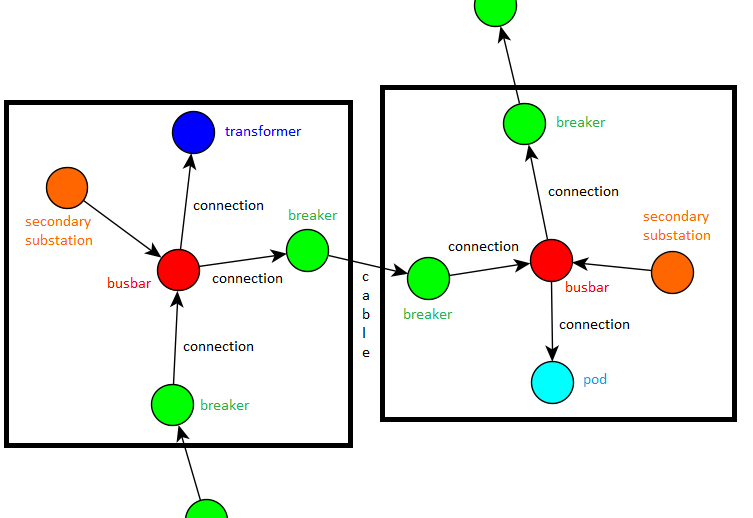
\includegraphics[scale=0.6]{chapters/figures/Secondary_substations.PNG}
    \caption{Detail of the elements of the electrical graph.}
    \label{fig:secondary-substations}
\end{figure}


\subsection{The substations graph}

The last graph we create is the \emph{substations graph}\index{substations graph}, a high-level, directed graph that models only the substations and their connections. We construct it by pruning the electrical graph of the other elements, so as to be able to inherit the connections among the substations and the direction of the power flow. In fact, a substation does not know either which are its elements, either which substations are before or after, only its components are connected among them. What we do is to cycle over all the elements, and for each type, we perform a specific action. Pods and transformers can be directly removed, since they are leaves in the electrical graph, so they can be deleted easily. To remove busbars and breakers, we create a new edge between their predecessor and their successor (being careful of creating it in the right direction), named with the \texttt{idsap}s of the two nodes at its ends separated by a dash, and then we remove them, which automatically removes also the edges connected to them. If everything is done in the right way, at the end we will have the edges among the substations labeled with their \texttt{idsap}s separated by a dash, first the parent's one and then the children's one. Then we compute the number of underlying users of each substation, summing the ones of each transformer or pod (in medium voltage) connected to it, and we store it in the node information.

In \autoref{fig:substations-graph} we can see a part of the substations graph, which is the computational model of the electrical diagram of \autoref{fig:mastrino}. Every node carries a lot of information about the substation, like its code, \texttt{idsap}, position, whether it is remotely controlled or not (labeled in bold and with an \texttt{R} in the figure if it is), and the number of users underneath it.

\begin{figure}[htbp]
    \centering
    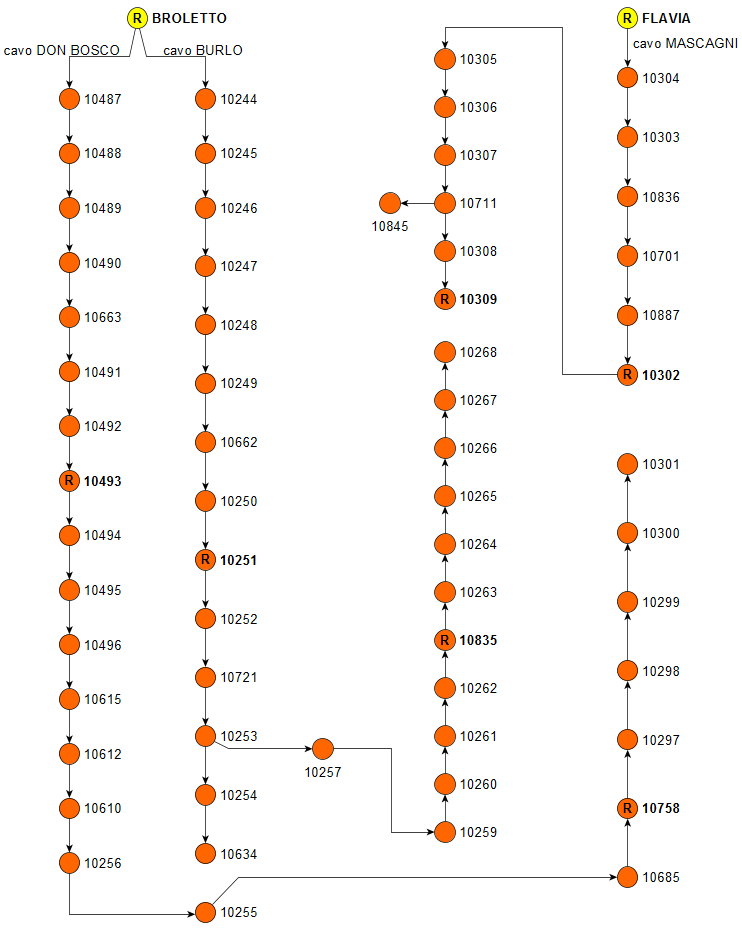
\includegraphics[scale=0.75]{chapters/figures/Substations_graph.PNG}
    \caption{Computational model of the electrical diagram of \autoref{fig:mastrino}. The substations with a bold label and with an \texttt{R} are the remotely controlled ones.}
    \label{fig:substations-graph}
\end{figure}


\section{Simulator}

The simulator is a class that creates a fault in a specific point of the power grid, or is given the position of a fault, and then using the substations graph can tell the questioner -- which will be one our algorithms --- both if the fault is before or after the current substation in which the technician is located, and how many substations can be reconnected from that substation. It encodes the information available to the technician through the different methods at their disposal to discover if the fault is before or after the substation in which they are, and the results of their actions in a substation.

To discover if the fault is before or after the currently visited substation, a function of the simulator computes the predecessors and the successors of the current substation; then it scans the graph, starting from each successor, looking for the fault, and, if it finds it, it returns the successor from which it started. If it finishes the graph, arriving in all the leaves, without finding the fault, it scans the graph from each predecessor upwards; and when it finds the fault it returns the predecessor from which it started. In this way, the simulator returns either the subsequent substation of the current one, indicating that the fault is after it, or the previous substation of the current one, indicating that the fault is before it.

Instead, to compute the list of substations that can be reconnected by operating in the current one, the function takes the output of the previous function, computes the list of predecessors of the current substation, and if the fault is in it, it starts from the current substation and visits all the subsequent ones till the end, adding all of them to a set which is returned at the end of the computation. If the fault is not in the predecessors, it is in the successors, so a traversal of the graph is made from the first remotely controlled substation until the current substation is reached, adding all these substations to a set and returning it at the end of the computation.


\section{Algorithms}


At the moment, in all our algorithms we use a simplified version of the power grid, which does not consider electrical line forks, in order to simplify the computations. Thus, we only feed our algorithms with rectilinear power lines.


\subsection{Bisection}

The bisection algorithm, which is actually a binary search algorithm, plus their experience, is what the technicians currently use to solve a fault and reconnect all the disconnected substations left out after the initial operations. We create a class that models this method, although of course not exactly, since we don't have their experience at our disposal. Our bisection algorithm, in fact, simply takes the number of currently disconnected substations and visits the one in the middle, always selecting the one on the left in case of ties. Then it uses the simulator to compute the set of remaining disconnected substations and selects another action until this set is empty. The technicians, instead, do not choose exactly the substation in the middle, but bend this rule based on many different factors, like how easy it is to enter a substation, whether it is day or night --- which also affects the first condition, the weather conditions, etcetera.

In order to be able to compare all our algorithms, we compute the performance measure\index{performance measure} $J_\pi(\boldsymbol \theta)$ also for the bisection algorithm. So, first of all, we have to compute the policy matrix. For each state, we compute the substation that the bisection would choose in that situation, and we encode it in the corresponding policy row as a one hot-vector in which that action has coefficient $1$, while all other actions that can be taken in that state have a $0$, as well as the inadmissible actions. Then we compute the matrix of $Q_\pi$ using equation \eqref{eq:Q-recursive} (in \autoref{sec:model-implementation} we will describe in detail how we do it) and we use it to compute the performance measure using equation \eqref{eq:J}.


\subsection{Bisection improved}

Since the bisection algorithm, in a tie, blindly chooses the substation to the left, we were curious about how an algorithm slightly better at handling these ties would perform. So we created a bisection algorithm that, when a tie happens, chooses to visit the substation nearer to the current position of the technician. The algorithm iteratively chooses an action and uses the simulator to compute the set of remaining disconnected substations until this set is empty, which means that all the substations have been reconnected, and therefore the fault is solved.

Also for this algorithm, we computed a policy matrix, using one-hot vectors as its rows to indicate which substation it would choose in that state. Given this matrix, we were able to compute the performance measure $J_\pi(\boldsymbol \theta)$ like for the bisection.


\subsection{Weighted bisection}

The weighted bisection is yet another variation of the bisection algorithm, which determines the halfway substation to be visited according to the weights assigned to every substation. The weight of a substation is related to the cost of a fault: it is computed as the distance of the substation from the current position of the technician --- as the time it takes, in seconds, to go there --- multiplied by the number of underlying users of that substation. Thus, the algorithm computes the weight of each currently disconnected substation and decides the substation to visit by taking the one which minimizes the absolute value of the difference between the sum of the weights of the previous substations and the sum of the weights of the subsequent ones.

An efficient way to do it is to compute two vectors of the cumulated sums of the weights: one by scanning the substations from left to right, and the other one by scanning them from right to left
(the latter done by flipping the initial vector, calculating the vector of the cumulated sums from left to right, and then flipping it again). Then we take the absolute value of their difference and we look for the index with the lowest value.

%\chapter{Data Collection}

\section{The Telegram bot}



\section{Synthetic Data Generation}

Synthetic data is ``any production data applicable to a given situation that are not obtained by direct measurement'' according to the McGraw-Hill Dictionary of Scientific and Technical Terms.

Given the total lack of data, I had to create them. We decided to use a Telegram bot which uses AWS to present to the technicians possible scenarios so to have record of what they would do to solve the power outage.


%\part{Reinforcement Learning} %{Algorithms}

\chapter{Reinforcement Learning} % {Theoretical foundations}
\label{chap:RL}


\section{Introduction}


As described in \cite{SuttonBarto}, Reinforcement Learning (\acrshort{rl}) is a paradigm of Machine Learning (\acrshort{ml}), along with others, like supervised learning and unsupervised learning. It analyzes how it is possible to learn the best course of action in an environment based on maximizing some given numerical reward. The learner is not told which actions to take, but learns empirically which are the ones that lead to a bigger reward. It is also possible that the current action influences not only the immediate reward, but also the next status of the environment, and, through that, all the other rewards to come. In this case, we speak of delayed reward, which, together with trial-and-error search, form the two distinctive features of \acrshort{rl}.

\begin{figure}[!ht]
    \centering
    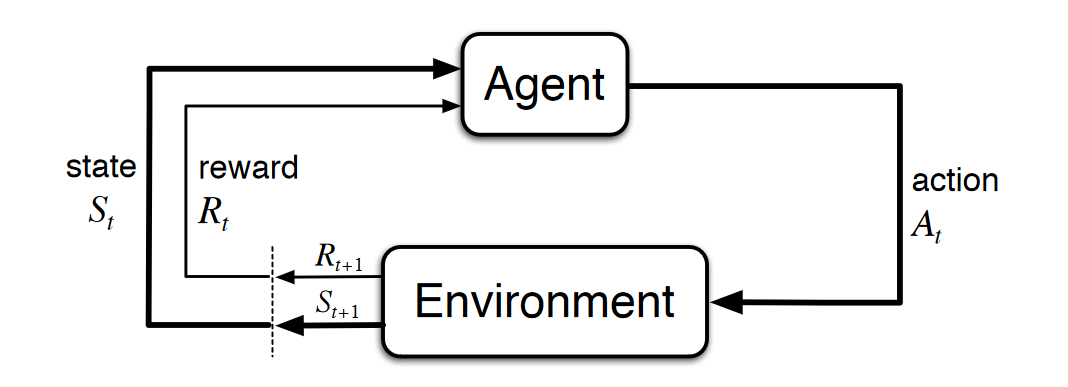
\includegraphics[width=0.9\textwidth]{chapters/figures/MDP-diagram.png}
    \caption{The agent-environment interaction \cite{SuttonBarto}}
    \label{fig:MDP}
\end{figure}

In an \acrshort{rl} problem we have a learning \emph{agent}\index{agent}, the decision-maker, that interacts over time with the \emph{environment}\index{environment} in which it is placed --- which includes everything outside the agent --- in order to achieve a \emph{goal}\index{goal}, which is to maximize the total reward it receives over the long run. As we see in \autoref{fig:MDP}, the agent can sense aspects of its environment through the \emph{states}\index{state} --- which can also be seen as a representation of the environment itself, it can choose \emph{actions}\index{action} to influence the environment, and it receives a \emph{reward}\index{reward} based on the outcome of its actions. We consider to be a reinforcement learning method any method that is well suited to solving problems framed in this way. Other elements of the \acrshort{rl} system are a \emph{policy}, a \emph{value function}, and a \emph{model} of the environment. A \emph{policy}\index{policy} describes the behavior of the agent at a given time, using a mapping from states to actions to be taken in those states. A \emph{value function}\index{value function} determines the value of a state as the total amount of reward an agent can expect to accumulate over the future, starting from that state. Instead, a \emph{model} of the environment\index{model of the environment} reproduces the behavior of the latter, and it is used for planning actions before actually experiencing them. For example, given to the model a state and action, it might predict with a certain probability the resultant next state and next reward.


\section{Finite Markov Decision Processes}

The treatment of this topic will closely follow the one presented in \cite{SuttonBarto}.

\emph{Markov Decision Processes}\index{Markov Decision Process}, or \acrshort{mdp}s, are used to formalize sequential decision-making, where actions influence the given rewards and the next states of the system, and through the latter also future rewards can be affected. Thus, \acrshort{mdp}s need to balance both immediate and delayed rewards. This formalism is used both in decision-theoretic planning (\acrshort{dtp}), \acrshort{rl}, and other learning problems in stochastic domains \cite{WierOtter12RLStateOfTheArt}.

We assume that the process evolves through a sequence of discrete time steps, $t = 1, 2, 3, \ldots$, even if it is possible to extend to the continuous case. These steps do not need to reflect fixed intervals of real time, but they can refer to arbitrary successive stages of decision-making and acting. At each time step $t$, the agent detects the \emph{state} of the environment, $S_t \in \mathcal S$, based on which it selects an action $A_t \in \mathcal A(s)$ (if the action set is the same in all states, we will write it simply as $\mathcal A$). Then, as a consequence, the agent receives, one time step later, a numerical reward $R_{t+1} \in \mathcal R \subset \mathbb R$, and ends up in a new state $S_{t+1}$. Thus, given this sequential process, it emerges a sequence, or \emph{trajectory}\index{trajectory}, given from
\begin{equation}
    S_0, A_0, R_1, S_1, A_1, R_2, S_2, A_2, R_3, S_3, \ldots
\end{equation}

In a \emph{finite} \acrshort{mdp}\index{finite MDP} we have that the set of states $\mathcal S$, actions $\mathcal A$, and rewards $\mathcal R$ have finite cardinalities, respectively $|\mathcal S|, |\mathcal A|$, and $|\mathcal R|$.

Since it is a \textit{finite} MDP, the random variables $R_t$ and $S_t$ have well-defined discrete probability distributions, and since we are considering a \textit{Markov} process, it holds the \emph{Markov property}, also called \emph{memorylessness property}, and thus the \emph{dynamics}\index{dynamics} of the process through the space of states, or the \emph{model} of the environment\index{model of the environment}, depend only on the preceding state and action:
\begin{equation}
    p(s', r \mid s, a) := \text{Pr}\{S_t = s', R_t = r \mid S_{t-1} = s, A_{t-1} = a\} \, ,
    \label{eq:transitions}
\end{equation}
for all $s', s \in \mathcal S$, $r \in \mathcal R$, and $a \in \mathcal A(s)$.

One could compute also the \emph{transition probabilities}\index{transition probabilities}, defined (with a little abuse of notation, since we continue to use the letter $p$) as
\begin{equation}
    p(s'|s, a) := \text{Pr}\{S_t = s' \mid S_{t-1} = s, A_{t-1} = a\} = \sum_{r \in \mathcal R} p(s', r \mid s, a) \, .
\end{equation}

The \emph{expected rewards}\index{expected reward} for state--action--next-action triples can be computed as $r: \mathcal S \times \mathcal A \times \mathcal S \to R$,
\begin{equation}
    r(s, a, s') := \mathbb E \left[ R_t | S_{t-1} = s, A_{t-1} = a, S_t = s' \right] = \sum_{r \in \mathcal R} r \cdot p(s', r | s, a) \, .
\end{equation}

The \acrshort{mdp} can also be seen as the tuple $(\mathcal S, \mathcal A, p, r)$, where $r = r(s,a,s')$ is the expected immediate reward that the agent receives for taking action $a$ in state $s$ \cite{Kaelbling1998, Uther2010}.

To describe how likely it is for an agent to take any given action from any given state, we use the notion of policy. A \emph{policy}\index{policy} is a class of probability distributions $\pi(a|s)$ over an action $a \in A(s)$ for each state $s \in \mathcal S$:
\begin{equation}
    \pi(a|s) = \text{Pr} \{A_t = a | S_t = s\} \, ,
    \label{eq:policy-theory}
\end{equation}
which describes the probability that the agent chooses that action being in that state at that time step $t$.

The agent's goal is to maximize the \emph{expected return}\index{expected return}, o \emph{cumulative reward}\index{cumulative reward|see {expected return}}, it receives in the long run given a certain policy $\pi$:
\begin{equation}
    \mathbb E [G_t] = \mathbb E_{p(\cdot,\cdot|s_t,a_t), \pi} \left[ \sum_{t=0}^\infty \gamma^t R_t \right].
    \label{eq:goal}
\end{equation}
where $\gamma \in [0,1]$ is the \emph{discount factor}\index{discount factor}, and it determines how much we value future rewards. With $\gamma = 0$ the agent considers only immediate rewards and discards future ones, while with $\gamma = 1$ the agent will take into account, in the same way, every reward it receives, considering a very long series of events.

Actually, we can take this average with respect to the distribution of rewards themselves, so as to ignore the dependency on the distribution of rewards. This is a distinctive property of the fact that we are working with a \textit{known model of the environment}. So, since we are only interested in optimizing averages, we do not care any longer about what is the actual distribution of the rewards. Thus, we can rephrase the agent goal as
\begin{equation}
    \mathbb E [G_t] = \mathbb E_{p(\cdot|s_t,a_t), \pi} \left[ \sum_{t=0}^\infty \gamma^t r(s, a, s') \right].
    \label{eq:goal-average}
\end{equation}

To reach its goal, the agent must estimate how good it is to be in a given state if it is following a certain policy. This value is stored in the \emph{(state-)value function}\index{value function}\index{state-value function|see {value function}}. Formally, the value of state $s$ under policy $\pi$ is
\begin{equation}
    V_\pi (s) := \mathbb E \left[ G_t \mid S_t = s \right] = \mathbb E \left[ \left. \sum_{t=0}^\infty \gamma^k R_t \, \right| \, S_t = s \right], \; \text{for all } s \in \mathcal S \, ,
\end{equation}
which is the expected return when starting in state $s$ and following policy $\pi$ thereafter. If there exists a terminal state\index{terminal state}, which causes the process to terminate if reached, its value is always zero.

Similarly, the value of taking action $a$ in state $s$ under policy $\pi$ is stored in the \emph{(state-)action value function}\index{action value function}\index{state-action value function|see {action value function}}, or \emph{quality}\index{quality|see {action value function}}, which is expressed with
\begin{equation}
    \begin{aligned}
        Q_\pi(s,a)
        &:= \mathbb E \left[ G_t \mid S_t = s, A_t = a \right] \\
        &= \mathbb E \left[ \left. \sum_{t=0}^\infty \gamma^k R_t \, \right| \, S_t = s, A_t = a \right],
    \end{aligned}
    \label{eq:Q}
\end{equation}
which is the expected return starting from state $s$, taking action $a$ and following policy $\pi$ thereafter.

We have that the following relation holds:
\begin{equation}
    V_\pi(s) = \sum_a \pi(a|s) Q_\pi(s,a) \, .
\end{equation}

The value function possesses a fundamental property, which is extensively used in \acrshort{rl}: it satisfies the following recursive relation
\begin{equation}
    \begin{aligned}
        V_\pi (s)
        &= \sum_a \pi(a|s) \sum_{s', r} p(s', r \mid s, a) \left[ r + \gamma V_\pi (s') \right] \\
        &= \sum_a \pi(a|s) \sum_{s'} p(s' \mid s, a) \left[ r(s,a,s') + \gamma V_\pi (s') \right] \, ,
    \end{aligned}
\end{equation}
which is called \emph{Bellman equation for $V_\pi$}\index{Bellman equation}.

Similarly, we have the \emph{Bellman equation for $Q_\pi$}:
\begin{equation}
    \begin{aligned}
        Q_\pi (s, a)
        &= \sum_{s', r} p(s', r \mid s, a) \left[ r + \gamma \sum_{a'} \pi(a'|s')  Q_\pi (s', a') \right] \\
        &= \sum_{s'} p(s' \mid s, a) \left[ r(s,a,s') + \gamma \sum_{a'} \pi(a'|s')  Q_\pi (s', a') \right] \, .
    \end{aligned}
    \label{eq:Q-recursive}
\end{equation}


\section{Partially Observable MDPs}

The presentation of this topic will mainly follow the one in \cite{Spaan12pomdp}.

What happens if the agent does not know anymore with full certainty the state of the environment, maybe due to imperfections or limitations in the agent's sensors, or to errors in the interpretation of the environment, or simply to unknown aspects of the environment itself?

If some features of the state are hidden from the agent, and the latter can sense only a part of the real state of the environment, the resultant state signal will no longer be Markovian, breaking a key assumption of most \acrshort{rl} methods, like the \acrshort{mdp} formulation. Luckily, we can consider an extension of the (fully observable) \acrshort{mdp} framework, that can deal with the uncertainty originating from the imperfect states perceived by the agent or the uncertain action effects.

A \emph{partially observable Markov decision process}\index{partially observable Markov decision process}, or \acrshort{pomdp}, is a framework that considers environments that are only partially observable to the agent, but allows anyway for optimal decision-making \cite{Kaelbling1998}, contrary to the requirement of full knowledge of the environment of \acrshort{mdp}s.

The fact that the environment is partially observable can derive mainly from two reasons:
\begin{itemize}
    \item different states generate the same observation, due to the same sensor reading, caused by the agent's limited knowledge of the environment;
    \item sensor readings are noisy, so the same state can generate different observations due to different sensor readings.
\end{itemize}
Thus, we have that the state of the environment is not uniquely identified by the agent's observations, and situations that appear similar to the agent may require instead different actions.

Interestingly, we can consider fully observable \acrshort{mdp}s as a special case of \acrshort{pomdp}s, in which the observation function maps each state to its correct unique observation deterministically \cite{Poupart2010}.

\begin{figure}[ht]
    \centering
    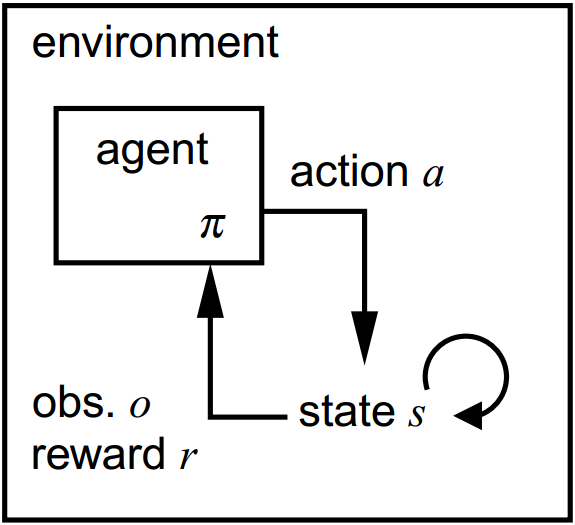
\includegraphics[width=0.45\textwidth]{chapters/figures/POMDP-schema.png}
    \caption{The agent-environment interaction in a POMDP \cite{Spaan12pomdp}}
    \label{fig:POMDP}
\end{figure}

Since a \acrshort{pomdp} is an extension of an \acrshort{mdp}, they share many elements. Also in \acrshort{pomdp}s the time is divided into different steps, and in each one of them the agent has to take an action. As for the \acrshort{mdp}s, we will consider discrete and finite models, which are simpler than the continuous ones. So the environment is represented with a finite set of states $\mathcal S = \{ s_0, s_1, s_2, \ldots, s_N \}$, and the finite set of possible actions is $\mathcal A = \{a_0, a_1, \ldots, a_K\}$. But instead of perceiving directly the state in which the environment is, the agent senses an \emph{observation}\index{observation} of it --- a signal that depends on the true state of the system but provides only partial information about it. The set of observations is discrete and finite: $\mathcal O = \{o_0, o_1, \ldots, o_M\}$, and represents all the possible sensor readings the agent can receive.

If the system is in state $s$ and the agent performs action $a$, we have that the system transitions to state $s'$ according to the transition probability $p(s' | s, a)$ as in a \acrshort{mdp}, but the agent receives observation $o'$ with probability
\begin{equation}
    z(a,s',o') = \text{Pr}(o' | a, s') \, ,
\end{equation}
using the notation of \cite{Poupart2010}.

\autoref{fig:POMDP} represents the interaction between these elements in the \acrshort{pomdp}.

Thus, a \acrshort{pomdp} can be described as the tuple $(\mathcal S, \mathcal A, p, r, \mathcal O, z)$, where $r = r(s,a,s')$ is the expected immediate reward, as in an \acrshort{mdp} \cite{Kaelbling1998}.

The goal of the agent is, once again, to find the optimal policy $\pi$ that maximizes the expected return\index{expected return} in \eqref{eq:goal-average}. To solve both \acrshort{mdp}a and \acrshort{pomdp}s, one can use several different methods, which are classified according to the dimensions of the state and action spaces, as well as based on whether the model of the environment is available or not. In fact, there are \emph{tabular methods}\index{tabular methods} --- which are exact and use arrays to store value functions, or \emph{approximate solution methods}\index{approximate solution methods} --- which employ function approximators, using limited computational resources; then there are \emph{model-based methods}\index{model-based methods} --- which make use of the known model of the environment and of planning to find the exact optimal policy, or \emph{model-free methods}\index{model-free methods} --- which are trial-and-error learner.

Often finding an exact optimal policy for \acrshort{pomdp}s can be computationally very expensive, so even for relatively small problems it is required to use approximate methods \cite{Aberdeen2002ScalingIP}. They are divided into two main classes: \emph{value-function methods}\index{value-function methods} --- or \emph{action-value methods}\index{action-value methods|see {value-function methods}} as in \cite{SuttonBarto}, that attempt to learn an approximate value function of the belief\index{belief} states (which are probability distributions over the states); and \emph{policy-based methods}\index{policy-based methods}, that search for a good policy within a fixed class of parameterized policies. We will focus on the second ones, since it is what we will implement to solve our problem.


\section{Policy gradient methods}
\label{sec:pgm}

A \emph{policy gradient method}\index{policy gradient method} is a policy-based method that attempts to optimize the parameters of a parametrized policy using either \emph{gradient  ascent}\index{gradient ascent} or \emph{gradient descent}\index{gradient descent} in the parameters' space, based on the expression of the agent's goal. In fact, it tries to maximize (or minimize) the expected return of a policy inside the policy class dictated by the parametrization. This method then uses directly the policy to choose the actions, instead of consulting a value function, which however might still be used to learn the parameters.

Policy gradient methods present some perks that make them highly valuable: the parametrized policy allows for direct incorporation of potential environment insights, they can naturally switch from the discrete setting to the continuous one, and they converge to at least a locally optimal policy, even if, as a drawback, the convergence can be very slow and finding the global optimum instead of a local one can be hard \cite{Peters2010}. Another distinctive trait of these methods is that they can also naturally handle partial state information. In fact, if a state variable can not be observed, then we can choose the policy parametrization such that the parameters do not depend on that state variable. Thus, we can directly apply these methods to \acrshort{pomdp}s, without having to make any changes.

We will denote the policy's parameters' vector with $\boldsymbol \theta \in \mathbb R^{d'}$, and we will write, as in \eqref{eq:policy-theory},
\begin{equation}
    \pi(a|s,\boldsymbol \theta) = \text{Pr}\{A_t = a | S_t = s; \boldsymbol \theta_t = \boldsymbol {\theta}\} \, ,
    \label{eq:policy-with-parameters}
\end{equation}
for the probability of taking action $a$ being in state $s$ at time $t$ with parameters $\boldsymbol \theta$ \cite{SuttonBarto}. The policy can be parametrized in any way, as long as it is differentiable with respect to its parameters, which means that the column vector of partial derivatives of $\pi$ w.r.t. the components of the parameters' vector $\boldsymbol \theta$, $\nabla_{\boldsymbol \theta} \pi (a|s,\boldsymbol \theta)$, exists and is finite for all $s \in \mathcal S, a \in \mathcal A$ and $\boldsymbol \theta \in \mathbb R^{d'}$. In particular, as described in \cite{Peters2010}, for discrete problems is often used the (exponential) soft-max distribution (i.e., Gibbs or Boltzmann distribution)
\begin{equation}
    \pi(a|s, \theta) = \frac{e^{\phi(s,a)^\top \theta}}{\sum_{b \in \mathcal A} e^{\phi(s,b)^\top \theta}} \, ,
    \label{eq:pi-boltzmann}
\end{equation}
while for continuous problems it is used the Gaussian distribution
\begin{equation}
    \pi(a|s, \theta) = \mathcal N(\phi(s,a)^\top \theta_1, \theta_2) \, ,
\end{equation}
where $\theta_2$ is an exploration parameter, and $\phi(s,a) \in \mathbb R^{d'}$ is a feature vector characterizing state $s$ and action $a$ \cite{Sutton2000}.

To learn the policy parameters $\boldsymbol \theta$, we will use the  gradient of some scalar \emph{performance measure}\index{performance measure} $J_\pi(\boldsymbol \theta)$ --- which can also be directly the expected return --- with respect to the policy parameters. If the performance $J_\pi(\boldsymbol \theta)$ measures the rewards that the agent receives, we want to maximize it, so we update the parameters approximating gradient \textit{ascent} in $J_\pi(\boldsymbol \theta)$:
\begin{equation}
    \boldsymbol \theta_{k+1} = \boldsymbol \theta_k + \alpha \nabla_{\boldsymbol \theta} J_\pi(\boldsymbol \theta_k) \, ;
    \label{eq:grad-ascent}
\end{equation}
instead, if the performance measures the costs that the agent encounters, we seek to minimize it, so we use approximate gradient \textit{descent} in $J(\boldsymbol \theta)$:
\begin{equation}
    \boldsymbol \theta_{k+1} = \boldsymbol \theta_k - \alpha \nabla_{\boldsymbol \theta} J_\pi(\boldsymbol \theta_k) \, ;
    \label{eq:grad-descent}
\end{equation}
where, in both cases, $\alpha > 0$ is a \emph{step-size parameter}\index{step-size parameter|see {learning rate}} or the \emph{learning rate}\index{learning rate}.

As done before, we will treat the episodic case, for which we define the \emph{performance measure}\index{performance measure} $J_\pi(\boldsymbol \theta)$ as the average value of the initial states\index{initial state} of the process:
\begin{equation}
    \begin{aligned}
        J_\pi (\boldsymbol \theta) 
        &= \sum_s \rho_0(s) V_{\pi_{\boldsymbol \theta}}(s) \\
        &= \sum_s \rho_0(s) \sum_a \pi(a|s) Q_{\pi_{\boldsymbol \theta}}(s, a) \, .
    \end{aligned}
    \label{eq:J}
\end{equation}
where we define as $\rho_0(s')$ the probability that an episode begins in state $s' \in \mathcal S$.

Let us define $\eta_\pi(s')$ as the average number of time steps that the agent spends in state $s'$ before the process dies. Time is spent in a state $s'$ if episodes start in that state $s'$, or if the environment transitions into $s'$ from a previous state $s$ in which time is spent. Thus, we have that the formula for $\eta_\pi$ is
\begin{equation}
    \eta_\pi(s') = \rho_0(s') + \sum_s \eta_\pi(s) \sum_a \pi(a|s) p(s'|s, a), \; \text{for all } s' \in \mathcal S.
    \label{eq:eta}
\end{equation}
This is a \textit{linear system} of equations, one for each state $s' \in \mathcal S$, and it can be solved for the expected number of visits $\eta_\pi(s)$.

The \emph{policy gradient theorem}\index{policy gradient theorem} provides an analytic expression for the gradient of the performance $J$ with respect to the policy parameters, which is what we need to approximate for gradient ascent in \eqref{eq:grad-ascent} (or descent in \eqref{eq:grad-descent}):
\begin{equation}
    \nabla_{\boldsymbol \theta} J(\boldsymbol \theta) = \sum_s \eta_\pi(s) \sum_a Q_\pi(s, a) \nabla_{\boldsymbol \theta} \pi(a|s).
    \label{eq:gradJ}
\end{equation}
See \cite{SuttonBarto} for the demonstration in the episodic case, which involves just elementary calculus and re-arranging of terms in the expression of the value function $V_\pi$.

Thus, solving the expression for \eqref{eq:gradJ} and using it in equations \eqref{eq:grad-ascent} -- \eqref{eq:grad-descent} allows optimizing the parameters of the policy, building an optimal policy in the chosen parametrization class. Note that to find both $\eta_\pi$ and $Q_\pi$ we need to solve two linear systems, \eqref{eq:Q-recursive} and \eqref{eq:eta}, and, moreover, they depend on the policy $\pi$, thus they must be solved at every iteration.


\subsection{Natural policy gradient}
\label{sec:npg}

In \cite{Amari1998}, it is introduced the \emph{natural gradient learning method}\index{natural gradient learning method}, which is a new way of performing a gradient descent algorithm for supervised learning problems, using a different formula for the gradient. This method is proved to be statistically efficient and does not get stuck in plateaus, like the conventional stochastic gradient learning does. This is because the ordinary gradient of a function, in some parameters spaces, does not identify its steepest direction, while the natural gradient does.

This method has also been applied in \acrshort{rl} in policy gradient algorithms \cite{Peters2008}, and where the improvements were made using the gradient $\nabla_{\boldsymbol \theta} J(\boldsymbol \theta)$ of the performance measure\index{performance measure} $J(\boldsymbol \theta)$, the \emph{natural gradient}\index{natural gradient} $\widetilde \nabla_{\boldsymbol \theta} J(\boldsymbol \theta)$ is used instead. The difference is that the first follows the steepest direction in the parameter space, while the latter follows the steepest direction with respect to the Fisher metric, given by
\begin{equation}
    \widetilde \nabla_{\boldsymbol \theta} J(\boldsymbol \theta) = F^{-1}(\boldsymbol \theta) \nabla_{\boldsymbol \theta} J(\boldsymbol \theta)
    \label{eq:natgradJ}
\end{equation}
where $F(\boldsymbol \theta)$ denotes the \emph{Fisher information matrix}\index{Fisher information matrix}. Since it can be proved that the angle between the two different gradients is never larger than ninety degrees, the convergence to the next local optimum is guaranteed. The natural policy gradient turns out to be significantly more efficient than normal gradients, since the convergence to the local minima is much faster.

The \emph{Fisher information}\index{Fisher information} is a metric which measures how much information a random variable $X$ carries about an unknown parameter $\theta$ that parametrizes the probability density function $f(X; \theta)$ of the variable $X$ itself. It has formula
\begin{equation}
    \mathcal F (\theta)
    = \mathbb E_\theta \left[ \left( \frac{\partial}{\partial \theta} \log f(X; \theta) \right)^2 \right]
    = \int_{\mathbb R} \left( \frac{\partial}{\partial \theta} \log f(x; \theta) \right)^2 f(x; \theta) \, dx \, .
    \label{eq:Fisher-information}
\end{equation}
If the density function $f(x; \theta)$ is at least twice differentiable with respect to the parameter $\theta$, and under certain regularity conditions, then the Fisher information may also be written as
\begin{equation}
    \mathcal F(\theta)
    = -\mathbb E_\theta \left[ \frac{\partial^2}{\partial \theta^2} \log f(X; \theta) \right] \, .
\end{equation}
The identity subsists as
\begin{align*}
    \frac{\partial^2}{\partial \theta^2} \log f(X; \theta)
    &= \frac{\partial}{\partial \theta} \left( \frac{1}{f(X; \theta)} \frac{\partial}{\partial \theta} f(X; \theta) \right) \\
    &= - \frac{1}{f(X; \theta)^2} \left( \frac{\partial}{\partial \theta} f(X; \theta) \right)^2 + \frac{1}{f(X; \theta)} \frac{\partial^2}{\partial \theta^2} f(X; \theta) \, ,
\end{align*} 
but
\begin{align*}
    \mathbb E_\theta \left[ \frac{1}{f(X; \theta)} \frac{\partial^2}{\partial \theta^2} f(X; \theta) \right]
    &= \int_{\mathbb R} \frac{1}{f(X; \theta)} \frac{\partial^2}{\partial \theta^2} f(X; \theta) \cdot f(X; \theta) dx
    = \int_{\mathbb R} \frac{\partial^2}{\partial \theta^2} f(X; \theta) dx \\
    &= \frac{\partial^2}{\partial \theta^2} \int_{\mathbb R} f(X; \theta) dx
    = \frac{\partial^2}{\partial\theta^2} 1 = 0 \, .
\end{align*}
% thus we have that
% \begin{align*}
%     \mathbb E_\theta \left[ \left( \frac{\partial}{\partial\theta} \log f(X; \theta) \right)^2 \right] &= \mathbb E_\theta \left[ \left( \frac{1}{f(X; \theta)} \frac{\partial}{\partial\theta} f(X; \theta) \right)^2 \right]
%     = \mathbb E_\theta \left[ \frac{1}{f(X; \theta)^2} \left( \frac{\partial}{\partial\theta} f(X; \theta) \right)^2 \right] =\\
%     &= - \mathbb E_\theta \left[ -\frac{1}{f(X; \theta)^2} \left( \frac{\partial}{\partial\theta} f(X; \theta) \right)^2 \right] + \mathbb E_\theta \left[ \frac{1}{f(X; \theta)} \frac{\partial^2}{\partial\theta^2} f(X; \theta) \right] =\\
%     &= -\mathbb E_\theta \left[ -\frac{1}{f(X; \theta)^2} \left( \frac{\partial}{\partial\theta} f(X; \theta) \right)^2 + \frac{1}{f(X; \theta)} \frac{\partial^2}{\partial\theta^2} f(X; \theta) \right] =\\
%     &= -\mathbb E_\theta \left[ \frac{\partial^2}{\partial\theta^2} \log f(X; \theta) \right]
% \end{align*}
Thus, we have that $\mathcal F(\theta)$ provides a measure of the intensity of the local curvature of the function $\log f(X; \theta)$ in a neighborhood of $\theta$: the larger $\mathcal F(\theta)$, i.e., the more pronounced the curvature of $\log f(X; \theta)$, the more concentrated the function $\log f(X; \theta)$ is around $\theta$, and the more information we have.

Consider the specific case of the soft-max policy \eqref{eq:pi-boltzmann}, where instead of defining the function $\phi(s,a)$, we take a parameter for each state $s$ and action $a$, $\theta_{s,a}$, obtaining a parameters' matrix $\boldsymbol \theta = (\theta_{s,a})_{s \in \mathcal S, a \in \mathcal A}$ (actually, it is a vector, but the visualization as a matrix is more convenient):
\begin{equation}
    \pi(a|s; \boldsymbol \theta) = \frac{e^{\theta_{s,a}}}{\sum_{d \in \mathcal A} e^{\theta_{s,d}}} \, .
\end{equation}
Following \cite{Hennes2020} (appendix A.4), we then define the Fisher information matrix\index{Fisher information matrix} $F$ of the previous policy $\pi_{\boldsymbol \theta}$ as $F(\boldsymbol \theta) = (F_{s,a,s',b})_{s,s' \in \mathcal S, a,b \in \mathcal A}$, where, for a specific state $s$,
\begin{equation}
    F_{a,b} = \sum_{c \in \mathcal A} \left( \frac{\partial}{\partial_{\theta_{s,a}}} \log \pi(c|s; \boldsymbol \theta) \right) \left( \frac{\partial}{\partial_{\theta_{s,b}}} \log \pi(c|s; \boldsymbol \theta) \right) \pi(c|s; \boldsymbol \theta) \, ,
    \label{eq:Fisher-matrix}
\end{equation}
in which we used the second equivalence of \eqref{eq:Fisher-information}.

First of all, we have that the gradient of the policy, $\nabla_{\boldsymbol \theta} \pi_{\boldsymbol \theta}$, has dimensions $(s', a') \times (s,a) \in (\mathcal S, \mathcal A) \times (\mathcal S, \mathcal A)$, and in particular the derivative of this policy, for a fixed state $s$, is
\begin{equation*}
    \begin{aligned}
        \frac{\partial}{\partial \theta_{s, a}} \pi(c | s; \boldsymbol \theta)
        &= \frac{\partial}{\partial \theta_{s, a}} \left(\frac{e^{\theta_{s,c} }}{\sum_{d \in \mathcal A} e^{\theta_{s,d} }} \right) \\
        &= \frac{\delta_{a,c} \cdot e^{\theta_{s,c} } \cdot \sum_{d \in \mathcal A} e^{\theta_{s,d} } -  e^{\theta_{s,c} } \cdot e^{\theta_{s, a} }}{(\sum_{d \in \mathcal A} e^{\theta_{s,d}})^2} \\
        &= \left(\frac{\delta_{a,c} \cdot e^{\theta_{s,c} } \cdot \sum_{d \in \mathcal A} e^{\theta_{s,d} }}{(\sum_{d \in \mathcal A} e^{\theta_{s,d} })^2} - \frac{e^{\theta_{s,c} }}{\sum_{d \in \mathcal A} e^{\theta_{s,d} }}\cdot\frac{e^{\theta_{s,a} }}{\sum_{d \in \mathcal A} e^{\theta_{s,d} }} \right) \\
        &= \left(\delta_{a,c} - \pi(a | s; \boldsymbol \theta) \right) \pi(c|s; \boldsymbol \theta)  \, .
    \end{aligned}
\end{equation*}
Thus, in this case, we have that
\begin{align*}
    F_{a,b}
    &= \sum_{c \in \mathcal A} \left( \frac{\partial}{\partial_{\theta_{s,a}}} \log \pi(c|s; \boldsymbol \theta) \right) \left( \frac{\partial}{\partial_{\theta_{s,b}}} \log \pi(c|s; \boldsymbol \theta) \right) \pi(c|s; \boldsymbol \theta) \\
    &= \sum_{c \in \mathcal A} \left( \frac1{\pi(c|s; \boldsymbol \theta)} \frac{\partial}{\partial_{\theta_{s,a}}} \pi(c|s; \boldsymbol \theta) \right) \left( \frac1{\pi(c|s; \boldsymbol \theta)} \frac{\partial}{\partial_{\theta_{s,b}}} \pi(c|s; \boldsymbol \theta) \right) \pi(c|s; \boldsymbol \theta) \\
    &= \sum_{c \in \mathcal A} \left( \frac1{\pi(c|s; \boldsymbol \theta)} \big( \delta_{a,c} - \pi(a|s; \boldsymbol \theta) \big) \, \pi(c|s; \boldsymbol \theta) \right) \left( \frac1{\pi(c|s; \boldsymbol \theta)} \big( \delta_{b,c} \right.\\
    & \qquad\qquad  - \pi(b|s; \boldsymbol \theta) \big) \, \pi(c|s; \boldsymbol \theta) \bigg) \pi(c|s; \boldsymbol \theta) \\
    &= \sum_{c \in \mathcal A} \big( \delta_{a,c} - \pi(a|s; \boldsymbol \theta) \big) \big( \delta_{b,c} - \pi(b|s; \boldsymbol \theta) \big) \pi(c|s; \boldsymbol \theta) \\
    &= \sum_{c \in \mathcal A} \big[ \big( \delta_{a,c} - \pi(a|s; \boldsymbol \theta) \big) \delta_{b,c} \pi(c|s; \boldsymbol \theta) - \big( \delta_{a,c} - \pi(a|s; \boldsymbol \theta) \big) \pi(b|s; \boldsymbol \theta) \pi(c|s; \boldsymbol \theta) \big]\\
    &= \big( \delta_{a,b} - \pi(a|s; \boldsymbol \theta) \big) \pi(b|s; \boldsymbol \theta) - \pi(b|s; \boldsymbol \theta) \pi(a|s; \boldsymbol \theta) + \pi(a|s; \boldsymbol \theta) \pi(b|s; \boldsymbol \theta) \sum_{c \in \mathcal A} \pi(c|s; \boldsymbol \theta) \\
    &= \big( \delta_{a,b} - \pi(a|s; \boldsymbol \theta) \big) \pi(b|s; \boldsymbol \theta) \, .
\end{align*}
This gives us, for a specific state $s$,
\begin{equation}
    F_{a,b} = \big( \delta_{a,b} - \pi(a|s; \boldsymbol \theta) \big) \pi(b|s; \boldsymbol \theta) = \frac{\partial}{\partial \theta_{s, a}} \pi(b | s; \boldsymbol \theta) \, ,
\end{equation}
which means that
\begin{equation}
    F = \nabla_{\boldsymbol \theta} \pi_{\boldsymbol \theta} \, ,
\end{equation}
and therefore we have that
\begin{equation}
    \widetilde \nabla \pi = F^{-1} \nabla_{\boldsymbol \theta} \pi_{\boldsymbol \theta} =  I_{(\mathcal S, \mathcal A) \times (\mathcal S, \mathcal A)} \, .
    \label{eq:nat-grad-pi}
\end{equation}

This is a very important result since it allows avoiding computing, and then inverting, the information matrix $F$, saving quite some computational time.

\chapter{Problem modelling and implementation}
\label{chap:model}


In this chapter, we are going to formulate our problem using the frameworks that we saw in \autoref{chap:RL}: we will define the basic elements, and then we will develop the formulas and the algorithm that we need to solve it.


\section{The mathematical model}

After a fault occurs and after the technician, together with the remote control room\index{remote control room}, restricts it to a limited number of non-remotely-controlled substations, the problem consists in visiting, and thus reconnecting, these substations in an order that minimizes the cost of the fault. We define the \emph{cost of the fault}\index{cost of the fault} as the amount of time each underlying user of each substation remains disconnected.

Thus, we are given a set of initially disconnected substations $\mathcal C$, with cardinality $|\mathcal C| = N$, between two remotely controlled substations, where these last ones will not be included in the set, since they are already reconnected. Looking at the electrical diagram\index{electrical diagram} of Trieste's power grid, we notice that the number of substations between two remotely controlled ones is always less than $20$, so we can say that in our problem $N < 20$. Luckily, this restricts the dimension of the problem.

\subsection{Elements of the POMDP}

Given that we don't know the position of the fault, but we have to find it while we reconnect the substations, we cannot use an \acrshort{mdp} to model this problem; instead, we will use a \acrshort{pomdp}. The \emph{agent}\index{agent} is the technician that has to decide which substation to visit at each step, while the \emph{environment}\index{environment} includes everything else, among which the possible positions of the fault, and the set of disconnected substations, and their positions and distances.

We define the \emph{state}\index{state} $s$ of the environment as the tuple
\begin{equation}
    s = (x_g, v_k, \{v\})
\end{equation}
where $x_g$ is the position of the fault, $v_k \in \mathcal C$ is the substation at which the technician is currently located, and $\{v\}$ is the set of substations still disconnected after the technician operates in the current substation $v_k$. The set $\{v\}$ can also be chosen to be the set of substations already reconnected, since they are complementary with respect to the set $|\mathcal C|$, but we chose to use the disconnected substations to ease the notation. Since the position of the fault is unknown, the variable $x_g$ is \emph{hidden}, while the variables $v_k$ and $\{v\}$ are \emph{observable}. When the fault occurs, the technician can be everywhere: at home if it happens in the middle of the night, at the company, or on the go. So we introduce an extra dummy substation, called substation $0$, which is the position of the technician when the fault occurs. Given this, we have that the \emph{initial state} is always of the form $s_0 = (x_g, 0, \mathcal C)$, thus we have different initial states, one for every possible position of the fault. Instead, a \emph{terminal state} is of the form $s_t = (x_g, v_k, \varnothing)$. If the fault is localized on an electrical cable, then $v_k$ is one of the two substations at the ends of that faulty cable, so we have two different terminal states; while if the fault is in a substation, $v_k$ is that exact substation, so the terminal state is only one. We notice that the initial cost has a random component, which depends on the position of the technician when the fault occurs, so on the position of the substation $0$. To remove this randomness, we could also impose that the technician position is always at the company, but we chose not to do that, in order to be closer to what really happens.

We then define the \emph{observation}\index{observation} $o$ that the agent senses from the environment as
\begin{equation}
    o = (v_k, \{v\}) \, ,
\end{equation}
and we will also write the state as $s=(x_g, o)$, where $o = (v_k, \{v\})$ is the observation itself. We define the observable $o$ to be a function of $s$:
\begin{equation}
    \begin{array}{cccc}
    o(s): & \mathcal S                                     & \rightarrow & \mathcal O       \\
          & s = (x_g, \, o = \left( v_k, \{v\} \right) \,) & \mapsto     & o = (v_k, \{v\})
\end{array} \, .
\end{equation}
For different states $s = (x_g, \, o = \left( v_k, \{v\} \right) \,)$ that differ only by the position of the fault $x_g$, this function associates the same observable $o = (v_k, \{v\})$. Thus, we have that $o$ is an equivalence class for $s$. For brevity, we will often keep this dependency implicit, and write simply $o$ instead of $o(s)$, meaning that $o = o(s)$. In particular, the observation of an initial state $s_0 = (x_g, 0, \mathcal C)$ is $o_0 = (0, \mathcal C)$.

We define the \emph{action}\index{action} $a$ that the agent can do as the choice of the specific substation the technician will visit as the next step, thus we have that $a \in \mathcal A = \mathcal C$. Actually, since the technician visits only disconnected substations, and never visits already visited substations, we have that $a \in \{v\}$, if we are in state $s = (x_g, v_k, \{v\})$. Thus, we have that the set of available actions depends on the current state:
\begin{equation}
    a \in \mathcal A \big( s = (x_g, v_k, \{v\}) \big) = \{v\} \, .
\end{equation}

We said that this is a problem with terminal states, which occur when we reconnect all the substations. A terminal state will always be reached, since with every action we visit a substation and can reconnect it, so at the very least we remove that substation from the set of disconnected substations. Actually, if we are lucky, each time we can remove half of the substations from the set of disconnected substations. We are therefore positive that the process terminates. So, for this specific problem, it doesn't make sense to introduce a discount factor $\gamma$ (therefore, we have that $\gamma = 1$ in the formulas of \autoref{chap:RL}).

Given all that, we have that the \emph{next state}\index{next-state} $s'$ of the environment is
\begin{equation}
    s' = (x_g, v_{k+1} = a, \{v'\}),
\end{equation}
where $\{v'\}$ is the set of disconnected substations after the technician operates in the substation $v_{k+1}$. Since the technician can always at least reconnect the substation they visit, the set of disconnected substations decreases after each action, so we have that $\{v'\} \subseteq \{v\} \backslash a$.

Finally, we define the \emph{expected reward}\index{expected reward} as the \emph{cost} of going to a certain substation (as the time, in seconds, it takes to go there from where the technician is) multiplied by the number of disconnected users. Let's define as $d_{v_k, v_{k+1}}$ the time in seconds to go from the substation $v_k$ to the next substation $v_{k+1}$, and as $n_{k}$ the number of users still disconnected \emph{before} operating in the substation $v_{k+1}$. So if we are in a state $s = (x_g, v_k, \{v\})$, we make an action $a$, and we end up in a state $s' = (x_g, v_{k+1} = a, \{v'\})$, we have that the number of disconnected users is
\begin{equation}
    n_{k} = \sum_{v \in \{v\}} u_v,
\end{equation}
where $u_v$ is the number of users underneath the substation $v$. So the expected reward has the following formula:
\begin{equation}
    r(s, a, s') = d_{v_k, a} \cdot n_{k} = d_{v_k, a} \cdot \sum_{v \in \{v\}} u_v \, ,
    \label{eq:expected-reward}
\end{equation}
even if it actually depends only on the previous state $s$ and the action taken $a$, but we will keep the term $s'$ to be consistent with the formulas of \cite{SuttonBarto}.
For now, in the cost we will ignore the cost of establishing if the fault is before or after the substation in which the technician is, which is complicated and might raise the total cost significantly. This is because we cannot properly model these costs, due to a lack of data on them. To improve the computation of the cost, we need to carefully take note of the operations the technicians perform when a fault occurs, and then expand the model. To carry out the data collection, one possibility is to implement a serverless Telegram bot using \acrshort{aws}.

In \autoref{fig:sequence-substations} we can see (part of) a trajectory (we miss the rewards) of our \acrshort{pomdp}, using a set of fictional substations.

\begin{figure}[!pht]
    \centering
    \begin{tabular}{cc}
        \subcaptionbox{
            A fault has occurred in $2 \mhyphen 3$. We are in substation $0$ and all the substations are disconnected (orange). Initial state: $s_0 = (2 \mhyphen 3, 0, \mathcal C = \{1,2,3,4,5\})$.
            \label{1} }
            {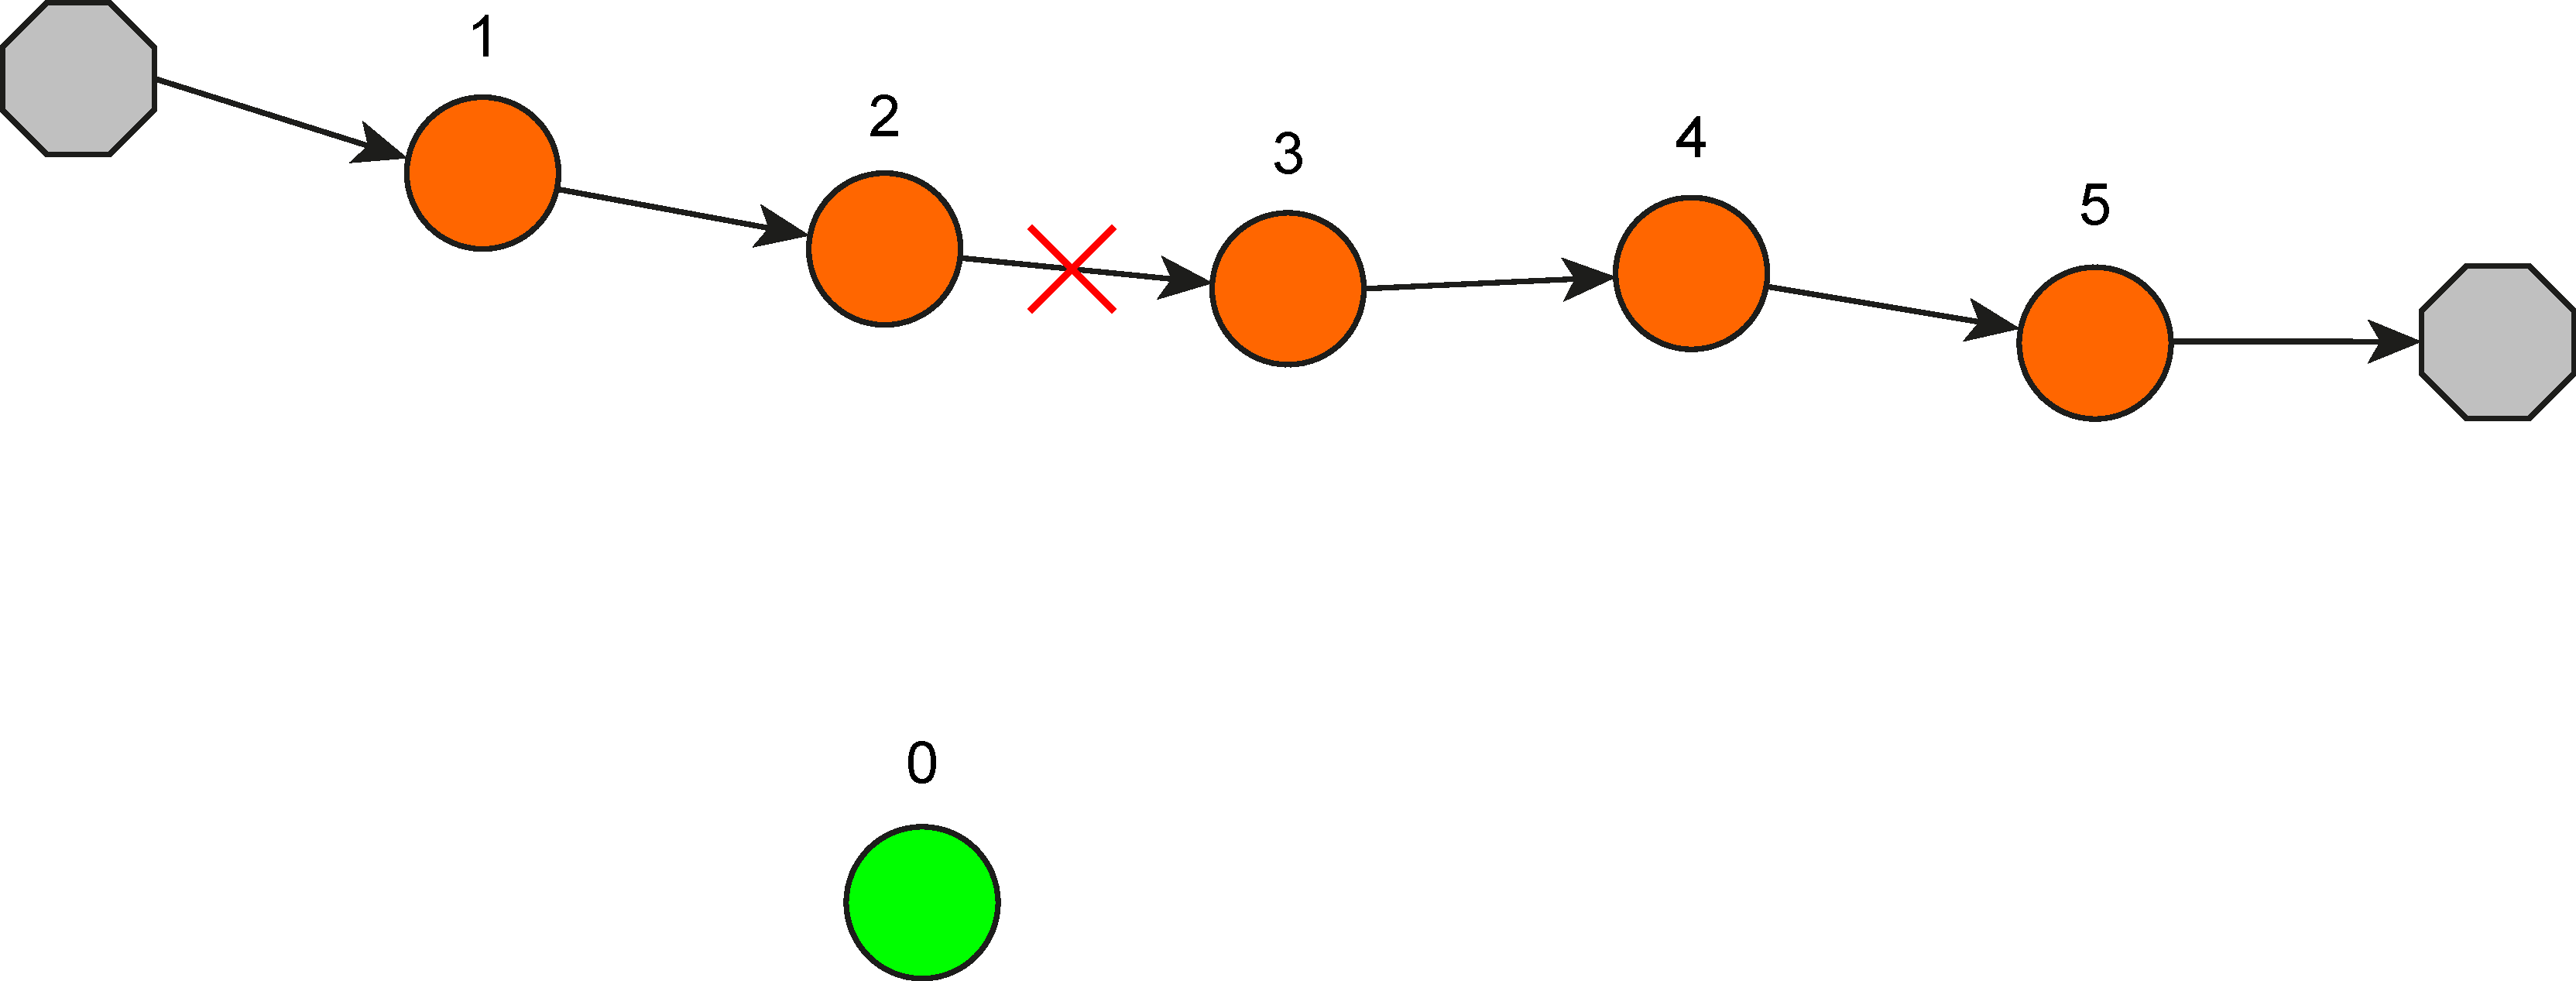
\includegraphics[width=0.45\textwidth,valign=b]{chapters/figures/POMDP_0.pdf}} &
        \subcaptionbox{
            We visit substation $4$ (yellow).\\ Action: $a_0 = 4$.
            \label{2}}
            {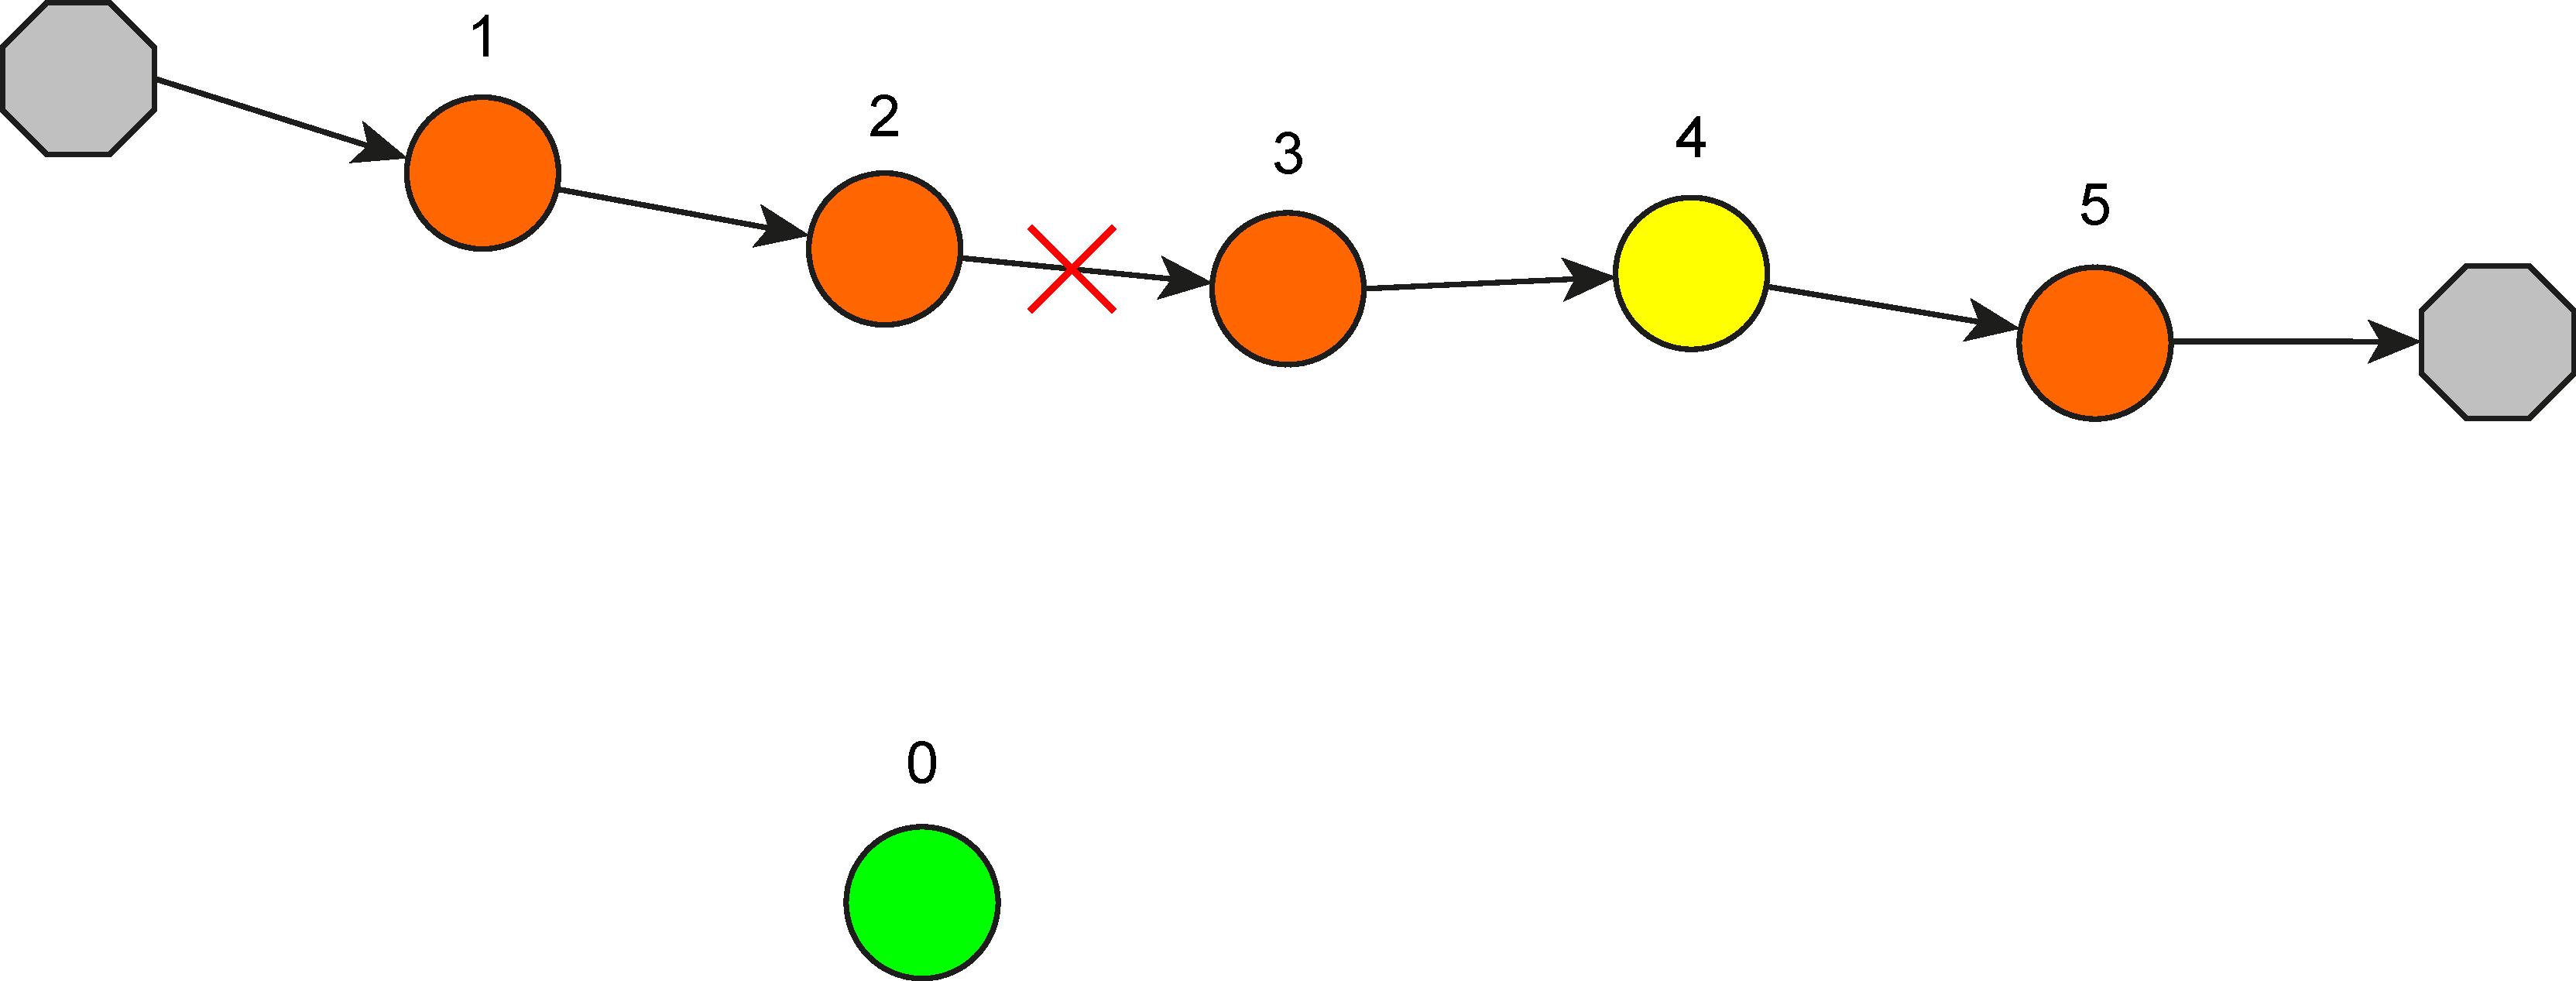
\includegraphics[width=0.45\textwidth,valign=b]{chapters/figures/POMDP_1.pdf}}\medskip\\
        \subcaptionbox{
            We reconnect substations $4$ and $5$ (green). State: $s_1 = (2 \mhyphen 3, 4, \{1,2,3\})$.
            \label{3}}
            {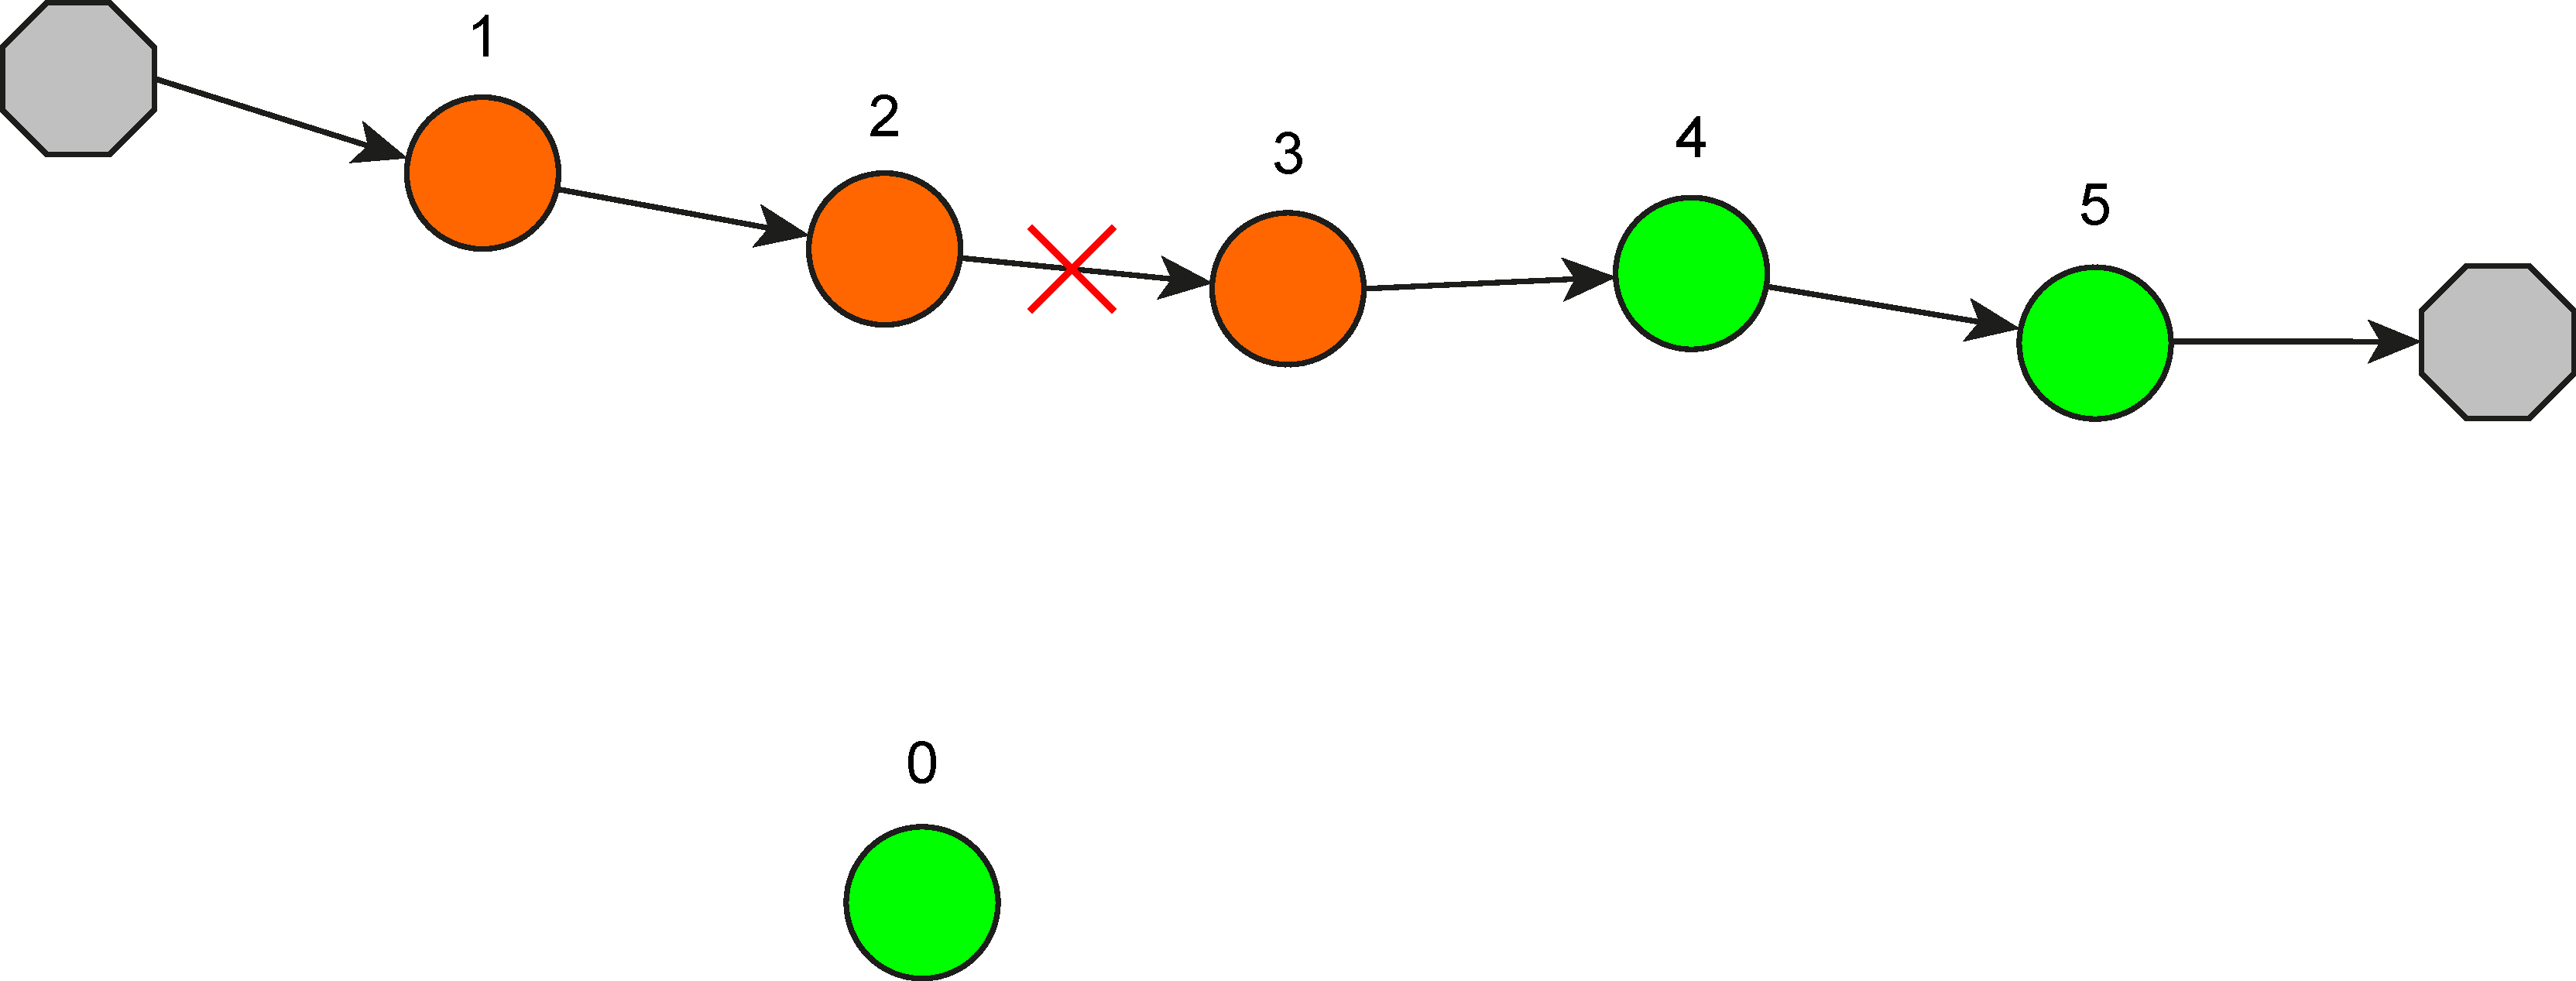
\includegraphics[width=0.45\textwidth,valign=b]{chapters/figures/POMDP_2.pdf}} &
        \subcaptionbox{
            We visit substation $3$ (yellow).\\ Action: $a_1 = 3$.
            \label{4}}
            {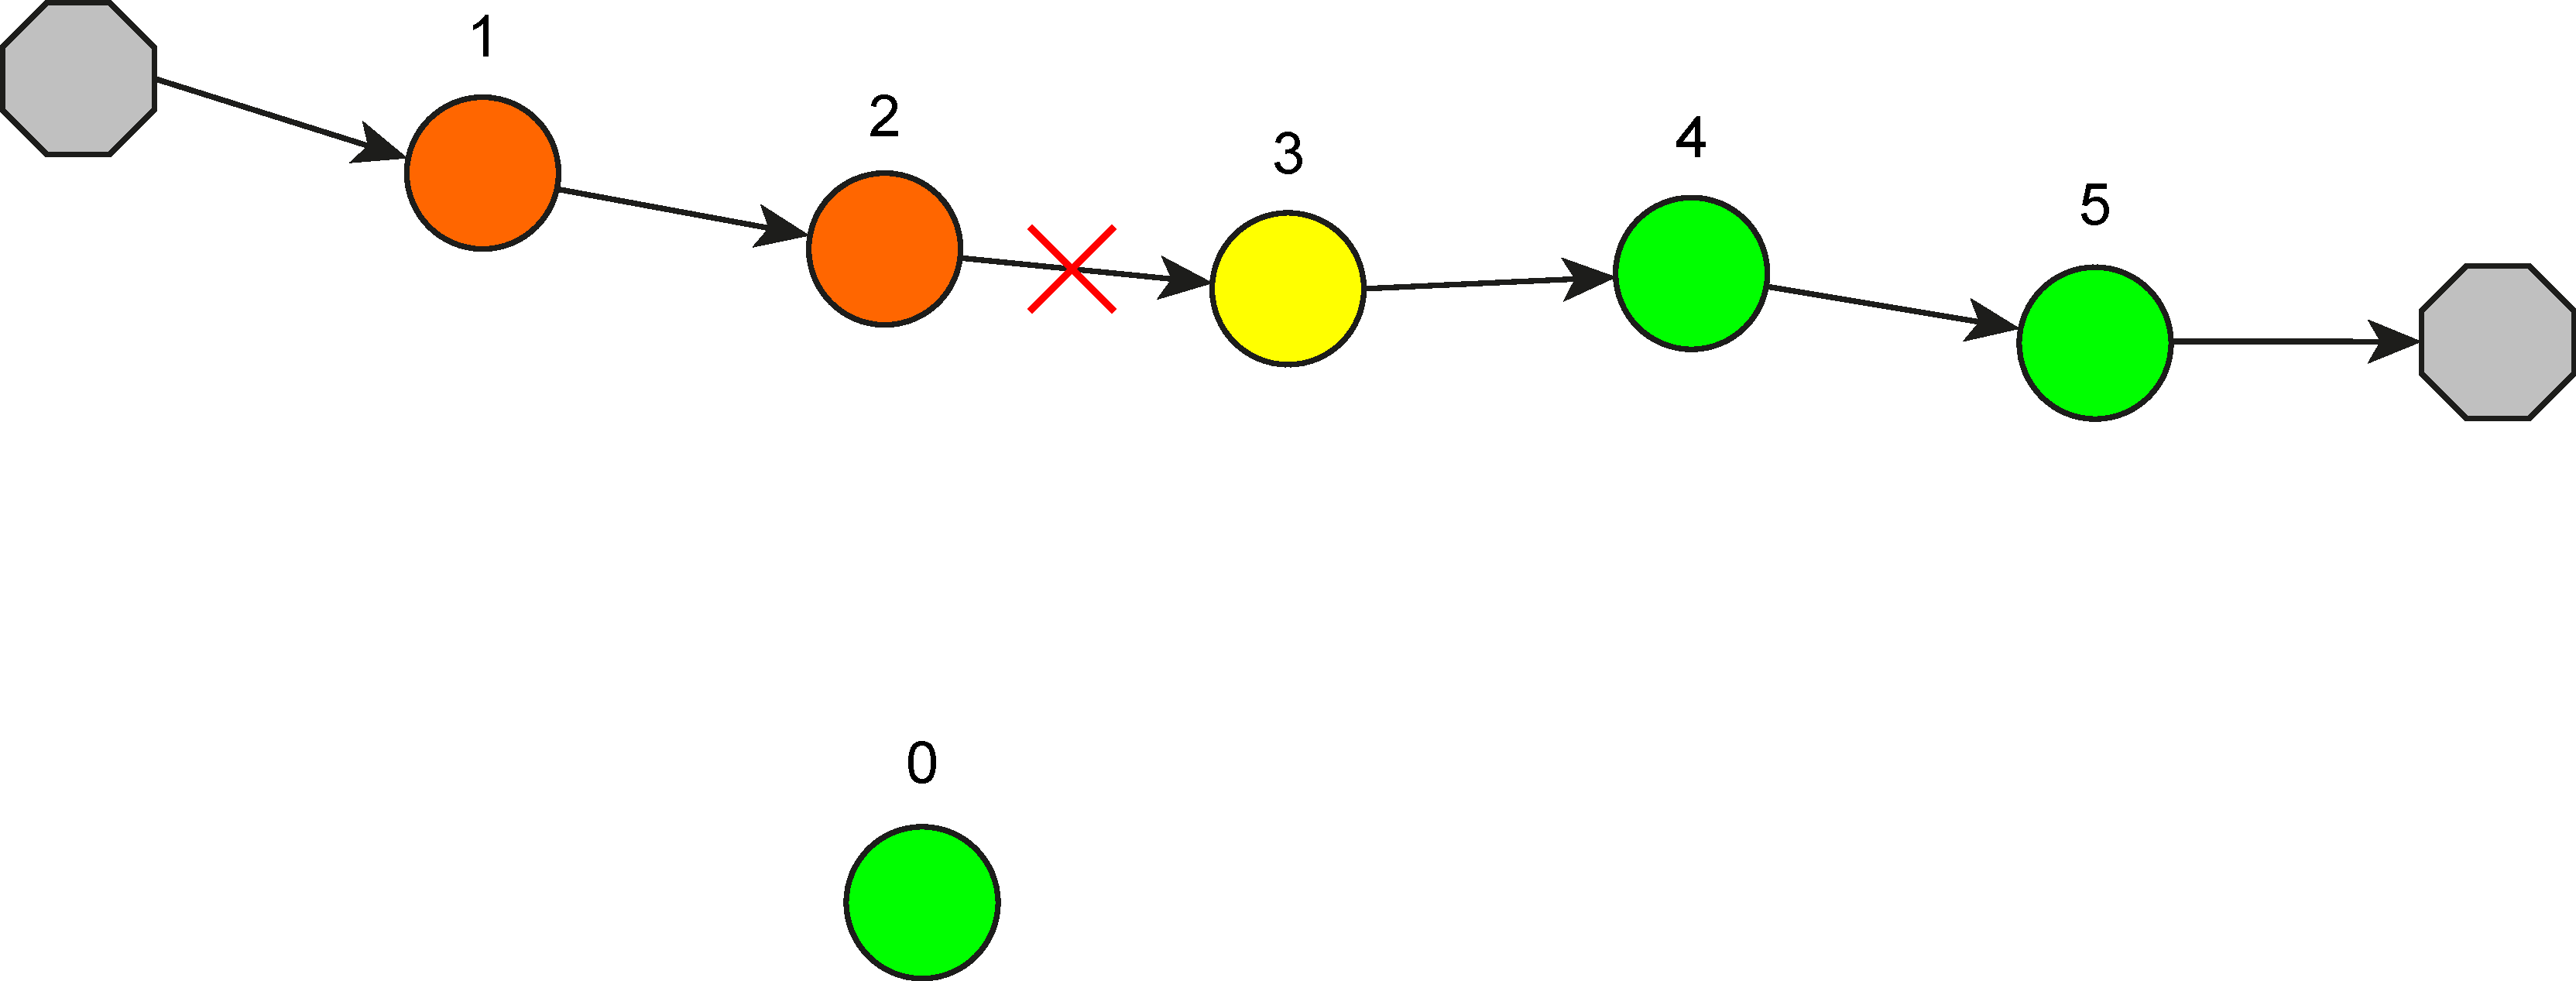
\includegraphics[width=0.45\textwidth,valign=b]{chapters/figures/POMDP_3.pdf}}\smallskip\\
        \subcaptionbox{
            We reconnect substation $3$ (green). State: $s_2 = (2 \mhyphen 3, 3, \{1,2\})$.
            \label{5}}
            {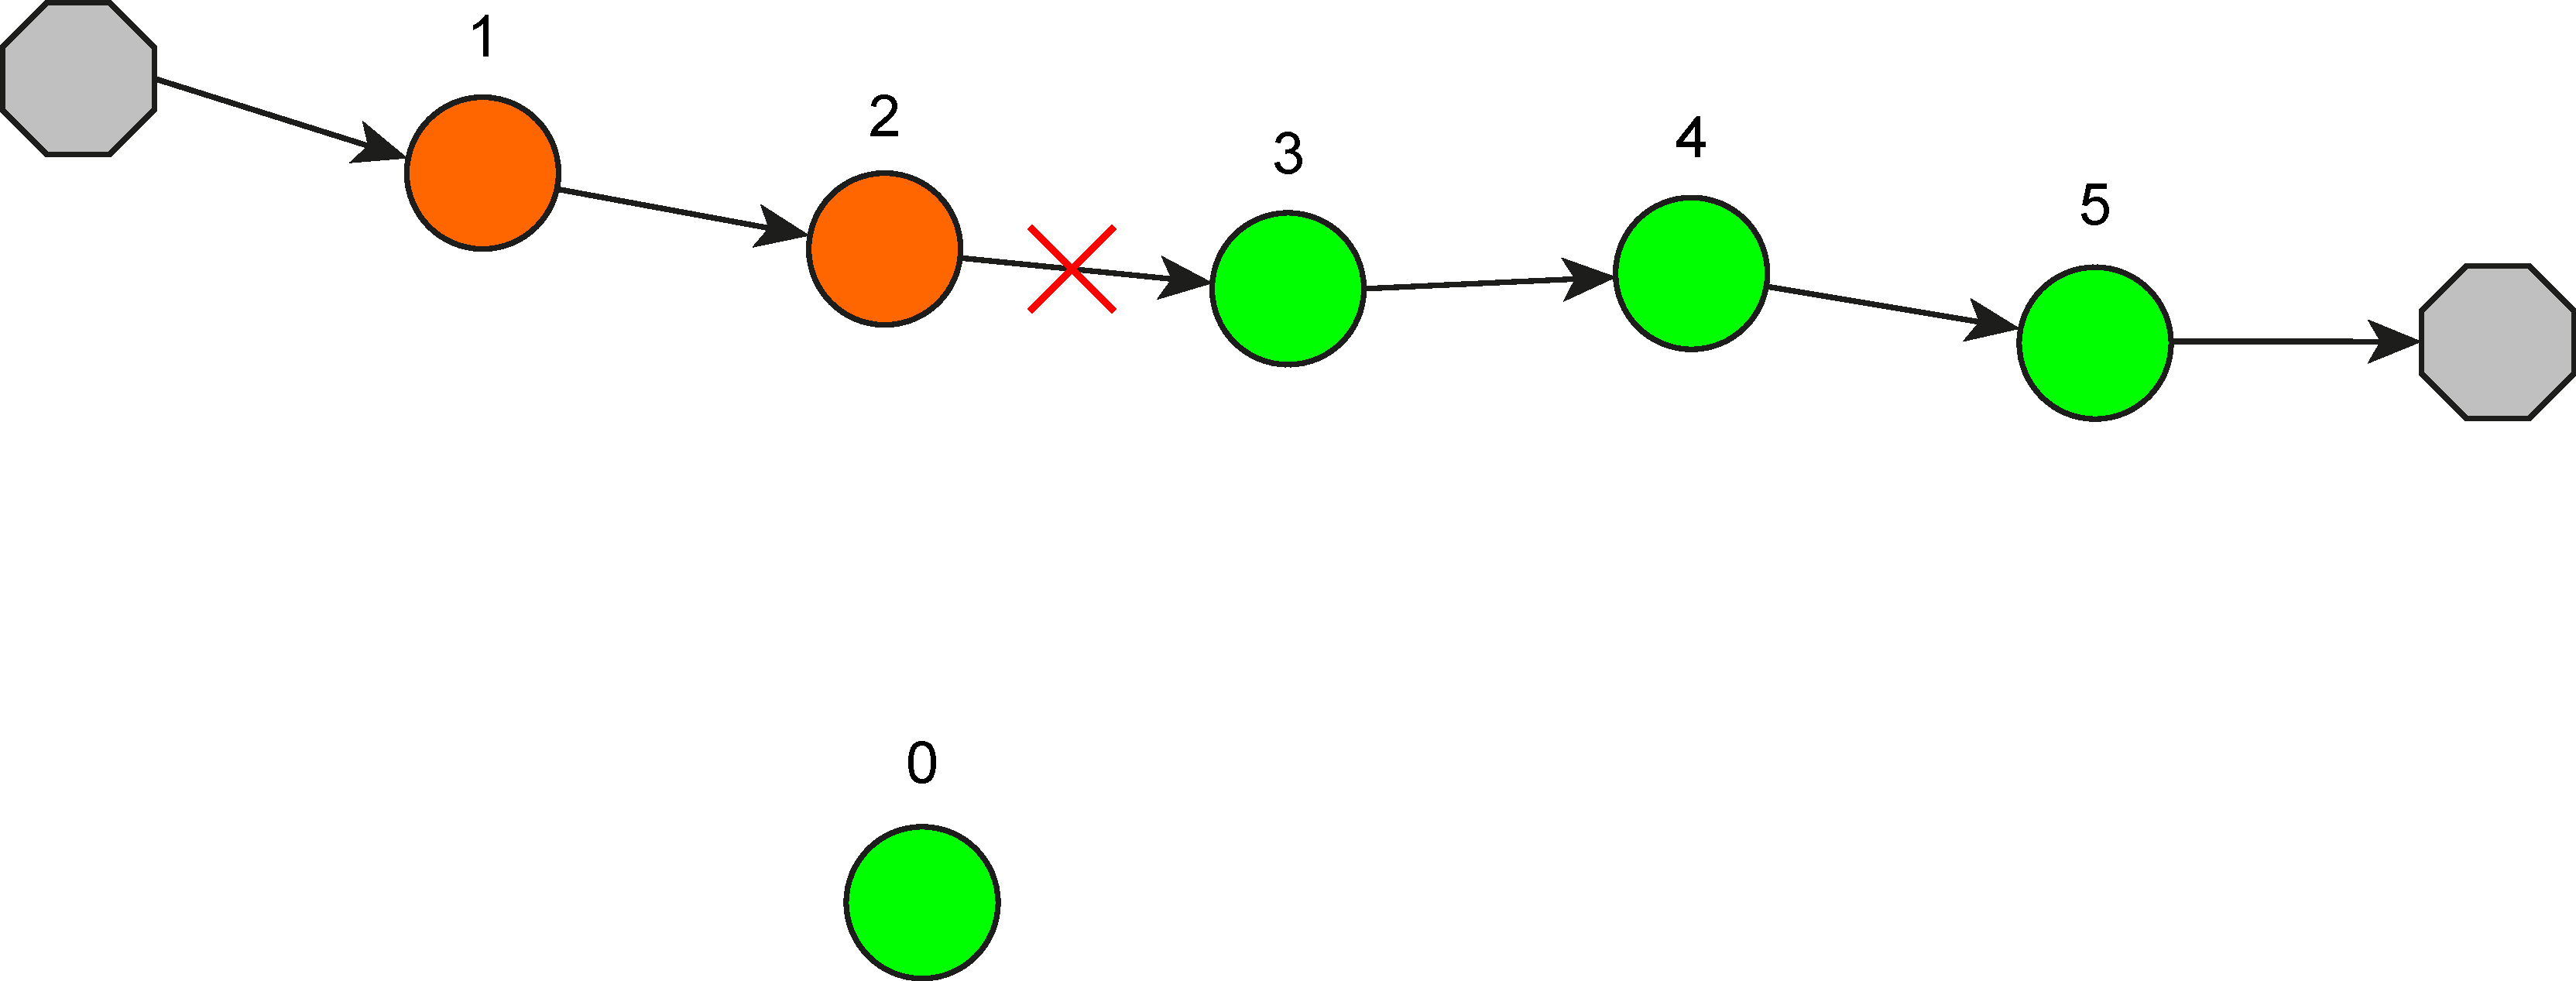
\includegraphics[width=0.45\textwidth,valign=b]{chapters/figures/POMDP_4.pdf}} &
        \subcaptionbox{
            We visit substation $2$ (yellow).\\ Action: $a_2 = 2$.
            \label{6}}
            {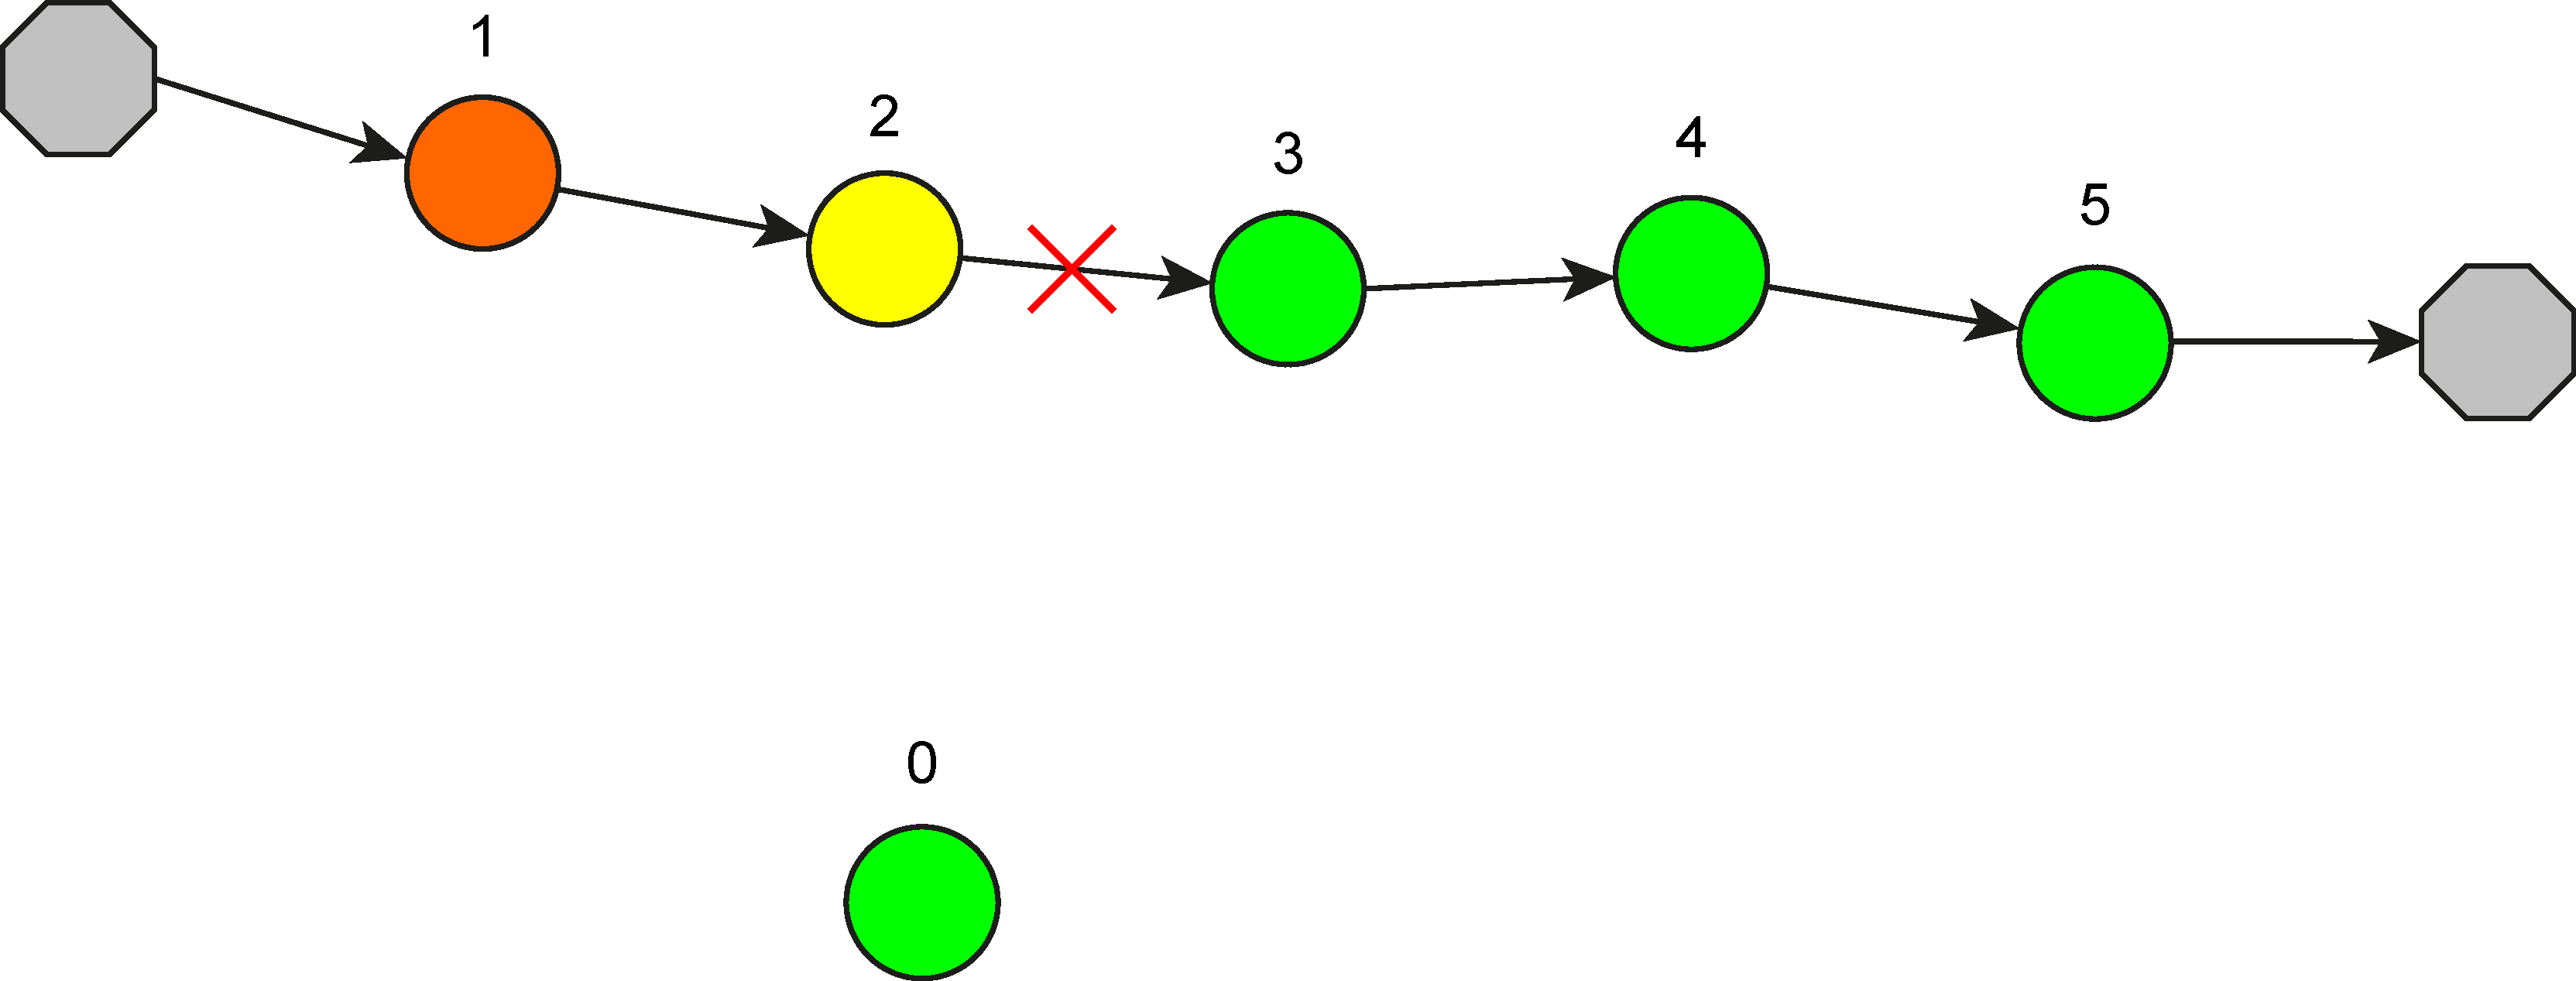
\includegraphics[width=0.45\textwidth]{chapters/figures/POMDP_5.pdf}}\medskip\\
    \end{tabular}
    \subcaptionbox{
        We reconnected substations $1$ and $2$ (green). All the substations are reconnected. Terminal state: $s_3 = (2 \mhyphen 3, 2, \varnothing)$.
        \label{7}}
        {\makebox[0.92\textwidth][c]{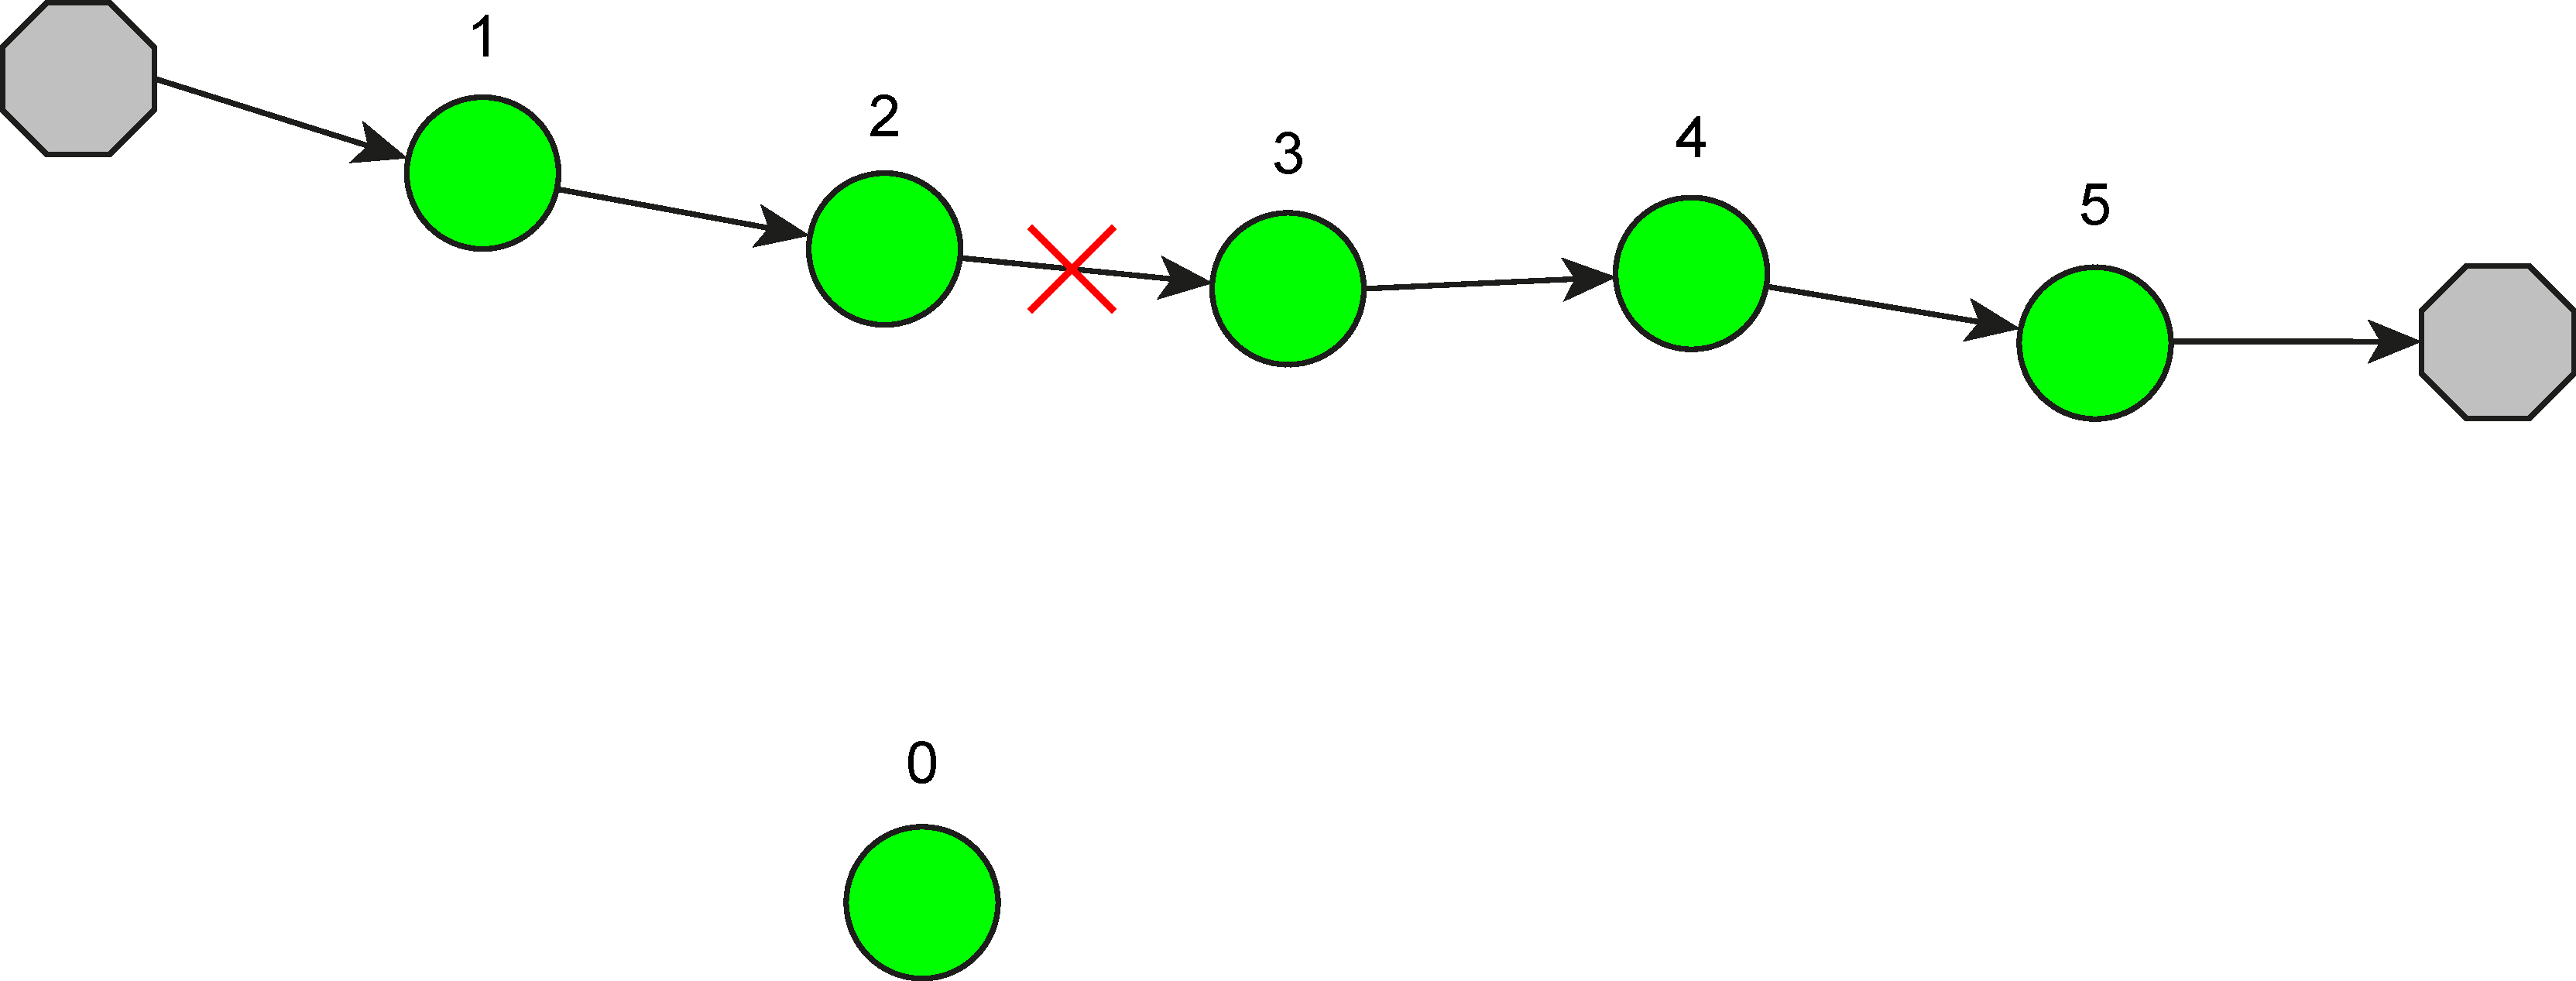
\includegraphics[width=0.45\textwidth]{chapters/figures/POMDP_6.pdf}}}
    \caption{Fictional example of the sequence of actions of the technician, from the occurrence of the fault to its resolution. The fault is in the electrical cable between substations $2$ and $3$, and the gray octagonal substations are the remotely controlled ones, while the round substations are the disconnected ones, except substation $0$, which is the initial position of the technician.}
    \label{fig:sequence-substations}
    \vspace{-17pt} % To remove warning that the image is too long
\end{figure}

The environment is \emph{deterministic}, so given an admissible action $a$, we will surely perform it and end up in the state to which that action leads. We can say that there are no execution errors, and we will always do what we want to do. This means that the next state $s'$ is a function of the previous state $s$ and the action $a$ performed: $s' = \sigma(s,a)$. So, mathematically, we have that the \emph{transition probability}\index{transition probability} is
\begin{equation}
    p(s' \mid s, a) = \mathbb I\big(s' = \sigma(s, a)\big) = \delta_{s', \sigma(s,a)} = \begin{cases} 1 & \text{if } s'=\sigma(s,a) \\ 0 & \text{otherwise} \end{cases} \,,
\end{equation}
where $\mathbb I$ is the characteristic function of a set, and $\delta$ is the Kronecker delta. In our specific case, the transition probability is equal to $1$ only when, starting from state $s = (x_g, v_k, \{v\})$, the new substation $v_{k+1}$ of the next state $s' = (x_g, v_{k+1}, \{v'\})$ is equal to the action $a \in \{v\}$ that we took, so:
\begin{equation}
    p(s' | s,a) = \begin{cases}
        1 & \text{if } v_{k+1} = a \\
        0 & \text{if } v_{k+1} \neq a
    \end{cases} \,.
    \label{eq:transprob}
\end{equation}


\subsection{Policy parametrization}

Given that we are in a situation of partial observability, as we don't know the position of the fault, the \emph{policy}\index{policy} depends only on the observables and not on the state, so it doesn't know where the fault is. Let's define a parameterized policy using a simple \emph{tabular} parameterization, in which we have a parameter $\theta_{o,a}$ for each observable $o$ and action $a$ pair:
\begin{equation}
    \boldsymbol \theta = (\theta_{o,a})_{o \in \mathcal O, a \in \mathcal A} = \begin{pmatrix}
        \theta_{o_1, a_1} & \theta_{o_1, a_2} & \cdots & \theta_{o_1, a_N} \\
        \theta_{o_2, a_1} & \theta_{o_2, a_2} & \cdots & \theta_{o_2, a_N} \\
        \vdots            &                   &        & \vdots            \\
        \theta_{o_{|\mathcal O|}, a_1} & \theta_{o_{|\mathcal O|}, a_2}  & \cdots &  \theta_{o_{|\mathcal O|}, a_N} \\
    \end{pmatrix}
\end{equation}
(where we recall that $N$ is the number of substations initially disconnected, so the number of possible actions: $|\mathcal A| = |\mathcal C| = N$).

Then we use the soft-max, or Boltzmann, distribution of \eqref{eq:pi-boltzmann} to construct the policy:
\begin{equation}
    \pi \Big( a \;\big|\; o(s) = (v_k, \{v\}); \boldsymbol \theta \Big) = \frac{e^{\theta_{o,a} }}{\sum_{b \in \{v\}} e^{\theta_{o,b} }} \,.
    \label{eq:parameterizedpolicy}
\end{equation}

So we have that also the policy is a matrix:
\begin{equation}
    \pi \Big( a \;\big|\; o(s); \boldsymbol \theta \Big) = \begin{pmatrix}
        \pi(a_1 | o_1; \boldsymbol \theta) & \pi(a_2 | o_1; \boldsymbol \theta) & \cdots & \pi(a_N | o_1; \boldsymbol \theta) \\
        \pi(a_1 | o_2; \boldsymbol \theta) & \pi(a_2 | o_2; \boldsymbol \theta) & \cdots & \pi(a_N | o_2; \boldsymbol \theta) \\
        \vdots            &                   &        & \vdots            \\
        \pi(a_1 | o_{|\mathcal O|}; \boldsymbol \theta) & \pi(a_2 | o_{|\mathcal O|}; \boldsymbol \theta)  & \cdots &  \pi(a_N | o_{|\mathcal O|}; \boldsymbol \theta) \\
    \end{pmatrix} \, .
\end{equation}
The policy cannot depend on the position of the failure, otherwise we would automatically have solved the problem: the policy would suggest going in the substation in which the fault is, or in the two substations at the ends of the faulty electrical cable.

Note that what matters in \eqref{eq:parameterizedpolicy} is not the absolute value of the parameters, but only the relative value of a parameter over another one: if we add a constant $c \in \mathbb R$ to all the parameters, there is no effect on the action probabilities, since the constant cancels out:
\begin{equation}
    \frac{e^{\theta_{o,a} + c}}{\sum_{b \in \{v\}} e^{\theta_{o,b} + c}}
    = \frac{e^c\cdot e^{\theta_{o,a} }}{e^c \sum_{b \in \{v\}} e^{\theta_{o,b}}}
    = \frac{e^{\theta_{o,a} }}{\sum_{b \in \{v\}} e^{\theta_{o,b} }}
    = \pi( a \mid o(s); \boldsymbol \theta) \, .
    \label{eq:policy-plus-constant}
\end{equation}
Initially, all parameters are the same and depend neither on the observation nor on the action (e.g., $\boldsymbol \theta = \mathbf 0$, thus $\theta_{o,a} = 0$ for all $o \in \mathcal O, a \in \mathcal A$), so that all actions have an equal probability of being selected. This is called the \emph{random policy}, and in our case is
\begin{equation}
    \pi \left( a \;\big|\; o(s); \boldsymbol \theta \right) = \frac{e^{\theta}}{\sum_{b \in \{v\}} e^{\theta}} = \frac{e^{\theta}}{e^\theta \sum_{b \in \{v\}} 1 } = \frac1{ |\{v\}| } \, ,
    \label{eq:rndpolicy}
\end{equation}
which means that we randomly choose a substation to visit, since they all have the same uniform probability. Actually, this is true for every choice of $\boldsymbol \theta$ which doesn't depend on the observation-action pair, so also any other constant $c \in \mathbb R$ would do (as we can see from \eqref{eq:policy-plus-constant}), but in practice, to construct a uniform policy, one usually takes $\boldsymbol \theta = \mathbf 0$.

One of the advantages of using the soft-max distribution to parameterize policies is that, in the learning phase, we are able to choose a random action without introducing and manually tuning a $\varepsilon$ term, which we would otherwise need to perform some exploration alongside the exploitation. Instead, the stochasticity is intrinsic, since we don't perform a deterministic maximization over the actions, but we choose it according to its probability. In particular, if the optimal policy is stochastic, an $\text{argmax}$ would never be able to approximate it, not even with a $\varepsilon$ parameter, while the soft-max can do it by construction. On the contrary, if an action is deterministic, the soft-max can approach it as close as possible; in fact, the approximate policy can approach a deterministic policy without any problem. 

If we search in this space of parametrized policies, this will give us a policy that doesn't depend on time, but only on the parameters, which we want to optimize. This means that, by construction, we have a \emph{stationary policy}. The reason for this choice is that, in our problem, the time is not encoded like a problem of dynamic programming, in which we have a well-defined sequence of time steps. The structure of the states is already a measure of time, as the number of moves already done: the sequence of substations we already visited. So what is important is not to establish a policy at different time steps, but to create a policy with respect to the states (in our case with respect to the observables).


\subsection{Value function and performance measure}

In our problem, the equation for the \emph{action value function}\index{action value function} $Q_\pi(s,a)$ in \eqref{eq:Q-recursive}, given that the state is $s = ( \, x_g, o = (v_k, \{v\}) \, )$, the action is $a \in \{v\}$ and the next state is $s' = ( \, x_g, o' = (v_{k+1}=a, \{v'\}) \, ) = \sigma(s,a)$ (since the system is deterministic), becomes, thanks to \eqref{eq:expected-reward} and \eqref{eq:transprob},
\begin{equation}
    \begin{aligned}
        Q_\pi(s,a)
        &= \sum_{s'} p(s' \mid s, a) \left[ r(s,a,s') + \sum_{a'} \pi(a'|o(s'); \boldsymbol \theta)  Q_\pi (s', a') \right] \\
        &= \left(d_{v_k, a} \cdot n_{k} + \sum_{a' \in \{v'\}} \pi \Big( a' \big| o \big( \sigma(s,a) \big); \boldsymbol \theta \Big) \, Q \big( \sigma(s,a), a' \big) \right) \, .
    \end{aligned}
    \label{eq:myQ}
\end{equation}

Now, let us find the formula for $\rho_0(s')$, the probability of starting in state $s'$. Since we have no prior information on where the fault might be, $\rho_0$ doesn't depend on it, so it will be uniform in $x_g$. The fault can happen either in one of the substations, which are $|\mathcal C| = N$, or on one of the electrical cables, which are $N+1$, so the number of possible $x_g$ is $N + (N+1) = 2N+1$. In an initial state, the current position of the technician $v_k$ must be the dummy substation $0$, which represents the position of the technician when the fault occurs, and the set of the disconnected substations must be equal to the set of all the substations $\mathcal C$. So $\rho_0$ must be $1$ when the current substation is $0$ and the set of the disconnected substations is equal to $\mathcal C$, and must be $0$ for every other situation. In other words, we have that
\begin{equation}
    \begin{aligned}
        \rho_0 \Big(s = ( \, x_g, o =(v_k, \{v\}) \,) \Big)
        &= \text{Pr}(x_g) \mathbb I (o = o_0 = (0, \mathcal C)) \\
        &= \frac1{2N+1} \mathbb I \big( v_k = 0, \{v\} = \mathcal C \big) \\
        &= \frac1{2N+1} \delta_{o(s), o_0} \, ,
    \end{aligned}
    \label{eq:myrho}
\end{equation}
where $o_0$ is the initial observation, and in the last equivalence we used the Kronecker delta $\delta$. Actually, according to the technicians of the \acrshort{aaa} company, the majority of the faults happens on the electrical cables, usually when they are no longer perfectly isolated. We will try to take advantage of this information at a later moment, but for now we will suppose that every component has the same probability of being damaged.

Moreover, the formula \eqref{eq:eta} for the function $\eta_\pi(s')$ in our case becomes, thanks to \eqref{eq:transprob} and \eqref{eq:myrho},
\begin{equation}
    \begin{aligned}
        \eta_\pi\Big(s' = (\, x_g, o'=(v_{k+1}, \{v'\}) \,) \Big)
        &:= \rho_0(s') + \sum_s \eta_\pi(s) \sum_a \pi(a | o(s); \boldsymbol \theta) p(s' | s, a) \\
        &= \frac1{2N+1} \delta_{o', o_0} + \sum_{s \in \mathrm{pa}(s')} \eta_\pi(s) \pi(v_{k+1} | o(s); \boldsymbol \theta) \, ,
    \end{aligned}
    \label{eq:myeta}
\end{equation}
where $\mathrm{pa}(s')$ indicates the parents of the node $s'$ in the states' dependency graph, which represents all the possible sequences of states.

Finally, let us define the \emph{performance measure}\index{performance measure} $J_\pi(\boldsymbol \theta)$ as the sum of all the costs we incur, added up over time until the process is concluded. Actually, the time steps of the process are merely formal steps, since we don't keep track of the time passed, but we simply move from one substation to another. Thus, the actual physical time is in the costs, as the cost of going from one substation to another, which we measure using the time it takes to drive between them. Given the definition of $J_\pi(\boldsymbol \theta)$ as in \eqref{eq:J}, in our case we have that
\begin{equation}
    \begin{aligned}
        J_\pi(\boldsymbol \theta) 
        &= \sum_s \rho_0(s) \sum_a \pi_{\boldsymbol \theta} (a|o(s); \boldsymbol \theta) \, Q_{\pi_{\boldsymbol \theta}}(s,a) \\
        &= \sum_{s} \frac{1}{2N+1} \delta_{o(s), o_0} \sum_a \pi_{\boldsymbol \theta} (a|o(s); \boldsymbol \theta) \, Q_{\pi_{\boldsymbol \theta}}(s,a) \\
        &=  \sum_{x_g} \frac{1}{2N+1} \sum_a \pi_{\boldsymbol \theta} (a|o_0; \boldsymbol \theta) \, Q_{\pi_{\boldsymbol \theta}} \big( (x_g, o_0),a \big) \, ,
    \end{aligned}
    \label{eq:myJ}
\end{equation}
where in the second equivalence we used equation \eqref{eq:myrho}, and the last equivalence derives from the fact that the sum $\sum_s \delta_{o(s), o_0}$ is equivalent to a summation over every possible position of the fault for the initial observation $o_0$. In particular, $(x_g, o_0)$ represents every possible initial state for different positions of the fault.


\subsection{Policy gradient method}

Since we know every aspect of the problem, and we have a model of the environment, we can solve it via a \emph{model-based method}\index{model-based method}. Due to the partial observability, though, we cannot use \emph{dynamic programming} methods like the ones in \cite{BellmanDP}, because we would need a policy that depends on the entire state, thus also on the hidden variable $x_g$. However, if we know where the fault is, the optimal solution is straightforward: if it is on an electrical cable, we need to visit the two substations at the ends of it (we might have to choose the right order); if it is in a substation, we visit it directly. Thus, we need an algorithm that can work in a \acrshort{pomdp}.

We will use one of the \emph{policy gradient methods}\index{policy gradient method} of \autoref{sec:pgm} in the \acrshort{pomdp}, since they can naturally handle partial observability. In particular, we will perform a \emph{gradient descent}\index{gradient descent} --- since we want to \textit{minimize} our \textit{cost} $J_\pi(\boldsymbol \theta)$ --- on the parameters $\boldsymbol \theta$ of the policy $\pi_{\boldsymbol \theta}$, where we said that the latter depends only on the observations, and so will do the gradient.

The formula of the gradient in \eqref{eq:gradJ} in our case becomes
\begin{equation}
    \nabla_{\boldsymbol \theta} J_\pi (\boldsymbol \theta) = \sum_{s \in \mathcal S} \eta_{\pi_{\boldsymbol \theta}}(s) \sum_{a \in \mathcal A(s)} Q_{\pi_{\boldsymbol \theta}}(s,a) \nabla_{\boldsymbol \theta} \pi(a|o(s); \boldsymbol \theta) \, .
    \label{eq:mygradJ_oneline}
\end{equation}

So, given that $\boldsymbol \theta$ is a matrix $\boldsymbol \theta = (\theta_{o,a})_{o \in \mathcal O, a \in \mathcal A}$, we have that also the gradient is a matrix:
\begin{equation}
    \nabla_{\boldsymbol \theta} J_\pi (\boldsymbol \theta) = \begin{pmatrix}
        \frac{\partial}{\partial \theta_{o_1, a_1}} J & \cdots & \frac{\partial}{\partial \theta_{o_1, a_N}} J \\
        \frac{\partial}{\partial \theta_{o_2, a_1}} J &  \cdots & \frac{\partial}{\partial \theta_{o_2, a_N}} J \\
        \vdots \\
        \frac{\partial}{\partial \theta_{o_{|\mathcal O|}, a_1}} J & \cdots & \frac{\partial}{\partial \theta_{o_{|\mathcal O|}, a_N}} J
    \end{pmatrix} \, ,
\end{equation}
where $N = |\mathcal A| = |\mathcal C|$ is the number of initially disconnected substations.

First of all, let us compute the gradient of the policy $\pi$. Given the equation of the policy in $\eqref{eq:parameterizedpolicy}$, we have that its derivative is
\begin{equation}
    \begin{aligned}
        \frac{\partial}{\partial \theta_{o',a'}} \pi \Big( a \;\big|\; o=(v_k, \{v\}); \boldsymbol \theta \Big)
        &= \frac{\partial}{\partial \theta_{o',a'}} \left( \frac{e^{\theta_{o,a} }}{\sum_{b \in \{v\}} e^{\theta_{o,b} }} \right) \\
        &= \delta_{o',o} \cdot \frac{\delta_{a',a} \cdot e^{\theta_{o,a} } \cdot \sum_{b \in \{v\}} e^{\theta_{o,b} } -  e^{\theta_{o,a} } \cdot e^{\theta_{o, a'} }}{(\sum_{b \in \{v\}} e^{\theta_{o,b}})^2} \\
        &= \delta_{o',o} \cdot \left( \frac{\delta_{a',a} \cdot e^{\theta_{o,a} } \cdot \sum_{b \in \{v\}} e^{\theta_{o,b} }}{(\sum_{b \in \{v\}} e^{\theta_{o,b} })^2} - \frac{e^{\theta_{o,a} }}{\sum_{b \in \{v\}} e^{\theta_{o,b} }}\cdot\frac{e^{\theta_{o,a'} }}{\sum_{b \in \{v\}} e^{\theta_{o,b} }} \right) \\
        &= \delta_{o',o} \cdot \left( \delta_{a',a} \pi(a|o; \boldsymbol \theta) - \pi(a|o; \boldsymbol \theta) \pi(a'|o; \boldsymbol \theta) \right) \\
        &= \delta_{o',o} \left( \delta_{a',a} - \pi(a'|o; \boldsymbol \theta) \right) \, \pi(a|o; \boldsymbol \theta)  \, ,
    \end{aligned}
    \label{eq:gradpi}
\end{equation}
since if $o \neq o'$ we have that $\theta_{o',a'}$ and $\theta_{o,a}$ are ultimately different parameters. In particular, for the random policy (so when $\boldsymbol \theta = \mathbf 0$) we have that
\begin{equation}
    \left. \frac{\partial}{\partial \theta_{o',a'}} \pi \Big( a \;\big|\; o=(v_k, \{v\}); \boldsymbol \theta \Big) \right|_{\boldsymbol \theta = \mathbf 0}
    = \delta_{o',o} \left(\frac1{|\{v\}|} \delta_{a',a} - \frac1{|\{v\}|^2} \right)
    \label{eq:deriv-pi}
\end{equation}
The gradient of the policy is, in general, a tensor with dimensions $|\mathcal O| \times |\mathcal A| \times |\mathcal O| \times |\mathcal A|$. For a fixed observation $o$ and for a fixed action $a$, however, it reduces to the following matrix:
\begin{equation}
    \nabla_{\boldsymbol \theta} \pi(a|o; \boldsymbol \theta) = \begin{pmatrix}
        \frac{\partial}{\partial \theta_{o_1,a_1}} \pi ( a | o; \boldsymbol \theta )
            %& \frac{\partial}{\partial \theta_{o_1,a_2}} \pi ( a | o; \boldsymbol \theta )
            & \cdots & \frac{\partial}{\partial \theta_{o_1,a_N}} \pi ( a | o; \boldsymbol \theta ) \\
        \vdots & &
        %&
        \vdots \\
        \frac{\partial}{\partial \theta_{o_{|\mathcal O|},a_1}} \pi ( a | o; \boldsymbol \theta ) 
            %& \frac{\partial}{\partial \theta_{o_{|\mathcal O|},a_2}} \pi ( a | o; \boldsymbol \theta )
            & \cdots & \frac{\partial}{\partial \theta_{o_{|\mathcal O|},a_N}} \pi ( a | o; \boldsymbol \theta ) \\
    \end{pmatrix}
\end{equation}

Given this, we have that
\begin{equation}
    \begin{aligned}
        \nabla_{\theta_{o',a'}} J_\pi (\boldsymbol \theta)
        &= \sum_{s \in \mathcal S} \eta_\pi(s) \sum_{a \in \mathcal A(s)} Q_\pi(s,a) \nabla_{\theta_{o',a'}} \pi(a|o(s)) \\
        &= \sum_s \eta_\pi(s) \sum_a Q_\pi(s,a) \delta_{o',o(s)} \Big( \big( \delta_{a',a} - \pi(a'|o(s)) \big) \, \pi(a|o(s)) \Big) \\
        &= \sum_{x_g} \eta_\pi \big((x_g, o') \big) \sum_a Q_\pi \big((x_g, o'),a \big) \big( \delta_{a,a'} - \pi(a'|o') \big) \, \pi(a|o') \, ,
    \end{aligned}
    \label{eq:mygradJ}
\end{equation}
where, as we did in equation \eqref{eq:myJ}, the sum $\sum_s \delta_{o', o(s)}$ is equivalent to a summation over every possible position of the fault for the specific observation $o'$ on which we are deriving. In particular, $(x_g, o')$ is the state with a fault at some position $x_g$ and with observation $o'$.

The idea of the algorithm is the following. We start from a certain policy, for example, the random policy of equation \eqref{eq:rndpolicy}, in which we choose randomly the substation to be visited. Then we compute the gradient for every parameter using \eqref{eq:mygradJ}. As we saw in \eqref{eq:deriv-pi}, the gradients of the policy are simple computations (since we decided the parametrization of the policy, we were able to derive their formulas), while the computations for the objects $Q_\pi$ and $\eta_\pi$ have to be done indirectly: we have to solve the linear equations \eqref{eq:myQ} and \eqref{eq:myeta} for the current policy, which can be more or less computationally heavy, also depending on the method chosen.
%Given the form of our transition probabilities $p(s' | s, a)$, we have that the equations of $Q_\pi$ do not depend on $s'$, but only on the current state $s$ and the action $a$. So, fixed the first state $s$, we have to solve two linear equations only on the actions (we can see the $Q(s,a)$ matrix as a series of vectors).

Having done these steps, we have the value of the gradient for every parameter. Then we take a step in the parameters space, and we descend the gradient. We stop when the value of $J_\pi (\boldsymbol \theta)$ doesn't change much in percentage.

In general, there is no guarantee that this is a convex problem in the parameters $\boldsymbol \theta$, on the contrary, we could have several minima. Therefore, we should perform different gradient descents starting with some policies different from the one which has $\boldsymbol \theta = \mathbf 0$, to see if we can reach a different minimum, or if we always reach the same one. These are called random restarts. Of course, this doesn't guarantee finding the global minimum, but it is the best we can do to at least check that we are not stuck in a local minimum. For the random restarts, we chose the parameters $\boldsymbol \theta$ from a standard normal distribution $\mathcal N(0,1)$, in order to have both positive values and negative ones to start from.

If we have the intuition that there is a deterministic sequence of actions to be performed, we have that their parameters $\theta_{\cdot,a}$ tend to infinity. This is because the deterministic policies correspond to a matrix of one-hot vectors --- in which we have $1$ for only one action and $0$ for all the other ones, which in the soft-max policy happens when the parameter associated with this action becomes much bigger than the others. If it is so, the gradient descent never stops and there could be problems of overflowing on the values of the policy, since the parameters $\boldsymbol \theta$ can become very large, and the exponentials of the soft-max would explode. A smart thing to do when this happens is to rewrite the parametrization in the following way (the observation $o$ is fixed):
\begin{equation}
    \pi(a | o) = \frac{e^{\theta_{o,a}}}{\sum_b e^{\theta_{o,b}}} = \frac{e^{-(\max_{a'} \theta_{o,a'} - \theta_{o,a})}}{\sum_b e^{-(\max_{a'} \theta_{o,a'} - \theta_{o,b})}} \, .
    \label{eq:pi-clipped}
\end{equation}
The benefit of writing the policy in this way is that, since the exponents of the two exponentials are negative (the parts in the parenthesis, $\max_{a'} \theta_{o,a'} - \theta_{o,\cdot}$, are always positive), it never explodes. In fact, negatives with large exponents ``saturate'' to zero rather than infinity, so we have a better chance of avoiding NaNs. This is a simple numerical trick that allows improving the stability of the algorithm. %([link](https://eli.thegreenplace.net/2016/the-softmax-function-and-its-derivative/))


\subsubsection{Natural policy gradient}

Following what we said in \autoref{sec:npg}, and given that the derivative of our policy is \eqref{eq:gradpi}, we have that

\begin{equation}
    \widetilde \nabla_{\theta_{o',a'}} \pi(a|o(s)) = I_{(\mathcal O, \mathcal A) \times (\mathcal O, \mathcal A)} = \delta_{o', o(s)} \delta_{a',a} \, .
\end{equation}

Then the equation of the natural gradient of the performance measure $J(\boldsymbol \theta)$ of \eqref{eq:natgradJ}, which was
\begin{equation*}
    \widetilde \nabla_{\boldsymbol \theta} J(\boldsymbol \theta) = F^{-1}(\boldsymbol \theta) \nabla_{\boldsymbol \theta} J(\boldsymbol \theta) \, ,
\end{equation*}
in our case becomes, thanks to the equation of the natural gradient of $\pi$ used in equation \eqref{eq:mygradJ_oneline},
\begin{equation}
    \begin{aligned}
        \widetilde \nabla_{\theta_{o',a'}} J_\pi (\boldsymbol \theta)
        &= \sum_{s \in \mathcal S} \eta_\pi(s) \sum_{a \in \mathcal A(s)} Q_\pi(s,a) \widetilde \nabla_{\theta_{o',a'}} \pi(a|o(s)) \\
        &= \sum_s \eta_\pi(s) \sum_a Q_\pi(s,a) \delta_{o', o(s)} \delta_{a',a} \\
        &= \sum_{x_g} \eta_\pi \big((x_g, o') \big) Q_\pi \big((x_g, o'), a' \big)\, .
    \end{aligned}
    \label{eq:mynatgradJ}
\end{equation}

This is a very nice result, in that we have a very simple equation for the gradient of the performance measure $J(\boldsymbol \theta)$, which is also guaranteed to converge faster to a minimum, although not a global one.


\section{Implementation of the model}

First of all, we generated all the states of the system using \emph{backtracking}\index{backtracking}, a technique used to systematically generate all the admissible solutions of a problem (usually of combinatorial nature) \cite{Montresor2014}. It proceeds by incrementally building candidate solutions using recursion, checking at each step if a complete and valid solution is reached, and backtracking to explore other ones. In our case, the function starts from a complete initial state, so, besides the current position of the technician and the set of disconnected substations, it also requires the position of the fault, and it determines all the possible actions that can be taken from that state. Then it computes all the subsequent states, determining each time which substations can be reconnected by doing one of the possible actions, and it continues until it has reconnected all the substations. We can reconstruct all the possible states of the system by looping over all the possible positions of the fault, so on all the possible initial states. While constructing the states, the function also creates the states' dependency graph, in which, given a state, we can find all the possible states in which we can end up doing an admissible action. This is actually a forest of trees: each graph is a tree because we can never return to a previous state, and it is a forest since the states are grouped by the position of the fault: if we start in a given initial state we can never end up in a state with a different position of the fault.

From the list of states, we create the list of observables, and we associate each state to its uniquely defined observation using a dictionary.

After having done that, we proceed to construct the matrix of parameters $\boldsymbol \theta$, initialized to zero, and the matrix of the policy $\pi_{\boldsymbol \theta}$, with the same dimensions of the previous one, using the soft-max parametrization.

Then we proceed with the computation of the matrix of $Q_\pi$. We construct the matrix $R = (R[s,a])_{s \in \mathcal S, a \in \mathcal A}$, which stores the immediate cost of being in state $s$ and doing action $a$, which thanks to \eqref{eq:expected-reward} is:
\begin{equation}
    R[s,a] = r(s,a,s') = d_{v_k, a} \cdot \sum_{v \in \{v\}} u_v \, ,
\end{equation}
if action $a$ is possible in state $s$, otherwise it is zero. Then we use it to initialize the matrix which will store the values of $Q_\pi$. Recall that in the equation \eqref{eq:myQ} for $Q_\pi$, we use the values of $Q_\pi$ of the next states $s'$ to compute the value of $Q_\pi$ for the current state $s$. Thus, we need to use the states' dependency graph from the leaves to the roots to compute the matrix of $Q_\pi$ bottom-up. We perform a personalized \emph{breadth-first-search}\index{breadth-first-search}, or \acrshort{bfs}, on the states' dependency graph, in order to be able to add each next-state contribution to the value of $Q_\pi$ for the current state. A breadth-first-search is an algorithm for exploring a graph, which visits every node and every edge of the latter. In a breadth-first-search, the nodes are visited in order of increasing distance from the source of the visit, where the distance among the source and a generic node is the minimum number of edges in a path among them \cite{Montresor2014}. In our modified \acrshort{bfs}, instead, we start from the terminal states in the leaves, and then we visit all the edges of the graph in a breadth-first-search order, with every edge traversed in the reverse direction in order to arrive at the initial state in the root. In particular, the major modification is that we visit all the out-edges of a node before visiting that node itself, in order to accumulate its $Q_\pi$ value --- by adding all the terms deriving from its children --- before using it to compute the $Q_\pi$ value of another node.

One might wonder why, being \eqref{eq:myQ} a linear system, we didn't use any of the already existing algorithms to solve it. This is because we don't have the matrix of the linear system explicitly, and we don't have an immediate way to create it, but it is required for algorithms like the Gauss elimination method (a direct method) or the Jacobi or Gauss-Seidel methods (iterative ones). So to compute it, we would need to first traverse the graph like we explained, writing the coefficients of the equations' terms of the linear system in $A$. Then we would still have to solve the linear system, for example with one of the previous methods. However, instead of doing these two passages, we can directly solve the system traversing the graph. This applies to the computation of $\eta_\pi$, as well.

After this, we proceed by computing the vector of $\eta_\pi$. In equation \eqref{eq:myeta} we have that, in order to compute the value of $\eta_\pi$ for a state $s'$, we use the values of $\eta_\pi$ of all its preceding states $s$. Thus, we will use the states' dependency graph from the roots to the leaves to compute the $\eta_\pi$ matrix top-down. As we did for the matrix of $Q_\pi$, we perform a modified \acrshort{bfs} on the states' dependency graph, which visits all the edges. Our \acrshort{bfs} visits a node only after all its in-edges have been visited; this ensures that we have accumulated the node's $\eta_\pi$ value, by having added all the terms deriving from its parents, before using it to compute the $\eta_\pi$ value of another node.

We could not have used a depth-first search, or \acrshort{dfs}, to compute $Q_\pi$ and $\eta_\pi$. In a \acrshort{dfs}, contrary to a \acrshort{bfs}, after visiting a node the search proceeds as far as possible from it along a path, until it reaches a node whose adjacent nodes have all already been visited. Then the search goes back along the last edge and continues moving along another path not yet visited \cite{Montresor2014}. Thus, using a \acrshort{dfs}, it would be impossible to visit all the in-edges (or the out-edges in the reverse order) of a node before visiting the node itself.

Having the matrix of the policy $\pi_{\boldsymbol \theta}$ and the matrix of $Q_\pi$, we can compute the performance measure $J_\pi (\boldsymbol \theta)$ using the last equivalence of \eqref{eq:myJ}. Instead, for the computation of the gradient of $J_\pi (\boldsymbol \theta)$, $\nabla_{\boldsymbol \theta} J_\pi (\boldsymbol \theta)$, we also use the matrix $\eta_\pi$, following equation \eqref{eq:mygradJ}. Since the convergence with the ordinary gradient was quite slow, we also implemented the natural gradient $\widetilde \nabla_{\boldsymbol \theta} J_\pi (\boldsymbol \theta)$, following equation \eqref{eq:mynatgradJ}. Given the higher values of $\boldsymbol \theta$ that the natural gradient can achieve, it is mandatory to implement the clipped version of the policy \eqref{eq:pi-clipped}.

How to choose the learning parameter $\alpha$\index{learning rate} appropriately? We want the difference $\boldsymbol \theta_{k+1} - \boldsymbol \theta_k$ in \eqref{eq:grad-descent} to be small; in particular, we want $\boldsymbol \theta_{k+1} - \boldsymbol \theta_k \ll 1$, therefore, we must have $\alpha \, |\nabla_{\boldsymbol \theta} J_\pi (\boldsymbol \theta)| \ll 1$. Given that we typically have $Q_\pi \sim 10^7$ and $\eta_\pi \sim 10^{-2}$ in the expression of $\nabla_{\boldsymbol \theta} J_\pi (\boldsymbol \theta)$, we choose $\alpha \sim 10^{-7}$. In our numerical runs, we actually used an adaptive $\alpha$ computed as $1 / \max(Q_\pi)$ at each iteration, in order to speed up the convergence and to avoid using a really small or big $\alpha$ with respect to the value of $Q_\pi$. This choice is still consistent with our previous argument; however, an adaptive $\alpha$ automatically takes into account the fact that the values of $Q_\pi$ increase when we have many initially disconnected substations.

After having computed all the elements that we need, we proceed to perform the gradient descent, stopping when the relative error among two subsequent values of $J_\pi (\boldsymbol \theta)$, normalized by $\alpha$, is less than $0.01\%$.

The pseudocode implementing our algorithm is shown in \autoref{alg:policy_gradient}.
% The ~ is used to avoid a line break between the two since they're considered a "single unit".

\begin{algorithm}
    \DontPrintSemicolon
    \caption{Policy gradient descent}
    \label{alg:policy_gradient}
        \KwData{The error tollerance: $\mathrm{tol} = 0.0001$}
        Initialize $\boldsymbol \theta = \mathbf 0$\;
        \Loop{
          Compute the matrix $\pi \gets \big( \pi ( a | o(s); \boldsymbol \theta ) \big)_{o \in \mathcal O, a \in \mathcal A}$\;
          Compute the vector $\eta \gets \big( \eta_\pi(s) \big)_{s \in \mathcal S}$\;
          Compute the matrix $Q \gets \big( Q_\pi(s, a) \big)_{s \in \mathcal S, a \in \mathcal A(s)}$\;
          $\alpha \gets 1/ \max(Q)$\;
          Compute $G \gets \nabla_{\boldsymbol \theta} J_\pi (\boldsymbol \theta)$ or $G \gets \widetilde \nabla_{\boldsymbol \theta} J_\pi (\boldsymbol \theta)$\;
          Compute $J \gets J_\pi (\boldsymbol \theta)$\;
          $\mathrm{error} \gets |J - J_\mathrm{old}|/J_\mathrm{old} \cdot 1/\alpha$ \;
          \If{$\mathrm{error}< \mathrm{tol}$}{
            \Break
          }
          Compute $\boldsymbol \theta \gets \boldsymbol \theta - \alpha G$\;
          Set $J_\mathrm{old} = J$
        }
\end{algorithm}

%\chapter{Linear programming}




%\part{Finance}

%\chapter{Automazione cabine}

% Valutare l'utilizzo del modello fatto per consigliare dove inserire nuovi elementi di automazione.

Dato il modello che simula la risoluzione del guasto e calcola il suo costo, aggiungi una simulazione aggiungendo una cabina telecomandata e vedi di quanto diminuisce il costo.

%\backmatter

\chapter{Results and conclusion}


In this chapter, we will comment on the results obtained with the algorithms we described in the previous chapters: we will both analyze them individually and compare them with each other. Then we will present our conclusions.


\section{Results}

% Dire cosa vogliamo andare a guardare per capire come fare meglio, se possiamo fare meglio, quindi ci serve una metrica; poi cominci a giustificare i parametri che abbiamo messo nelle simulazioni; dai qualche indicazione operativa e poi inizi a commentare i risultati.

We implemented firstly the ordinary policy gradient descent (\acrshort{pg}), using the formula for the gradient $\nabla_{\boldsymbol \theta} J_\pi (\boldsymbol \theta)$ in equation \eqref{eq:mygradJ}. Then, realizing how slow the convergence was, we decided to implement also the natural policy gradient algorithm (\acrshort{npg}), following equation \eqref{eq:mynatgradJ}. While reaching the same policy (the difference is in the order of $10^{-2}$), the \acrshort{npg} reaches convergence incredibly faster than the \acrshort{pg} algorithm, as we can see from the right panel of \autoref{fig:times}. From the left panel, which reports the same times but in logarithmic scale, we can see that both the two curves are exponentials, with approximately the same rate, but the \acrshort{npg} one has an initial value about $10^{-2}$ times smaller than the \acrshort{pg} one, which considerably reduces the computation time.
% ab^x, cd^x -> log(ab^x), log(cd^x) -> log(a)+xlog(b), log(c)+xlog(d) -> log(b) = log(d), log(a) != log(c)

These two algorithms find a policy that is not completely deterministic: in fact, some states have a stochastic policy over their possible actions. This means that we are on a side of the simplex which represents the policy space, and not in a corner. However, if, given a fault, we follow the actions dictated by the policy, we end up only in states with a deterministic choice of the action to be performed. In particular, an interesting thing to notice is that in the initial state the policy always tells to go to the substation in the middle, like the bisection algorithm. Then, for subsequent substations, the two policies began to differ, giving very different results, as we will see later.

\begin{figure}[t]
    \centering
    \mbox{
        \hspace*{-19.5pt}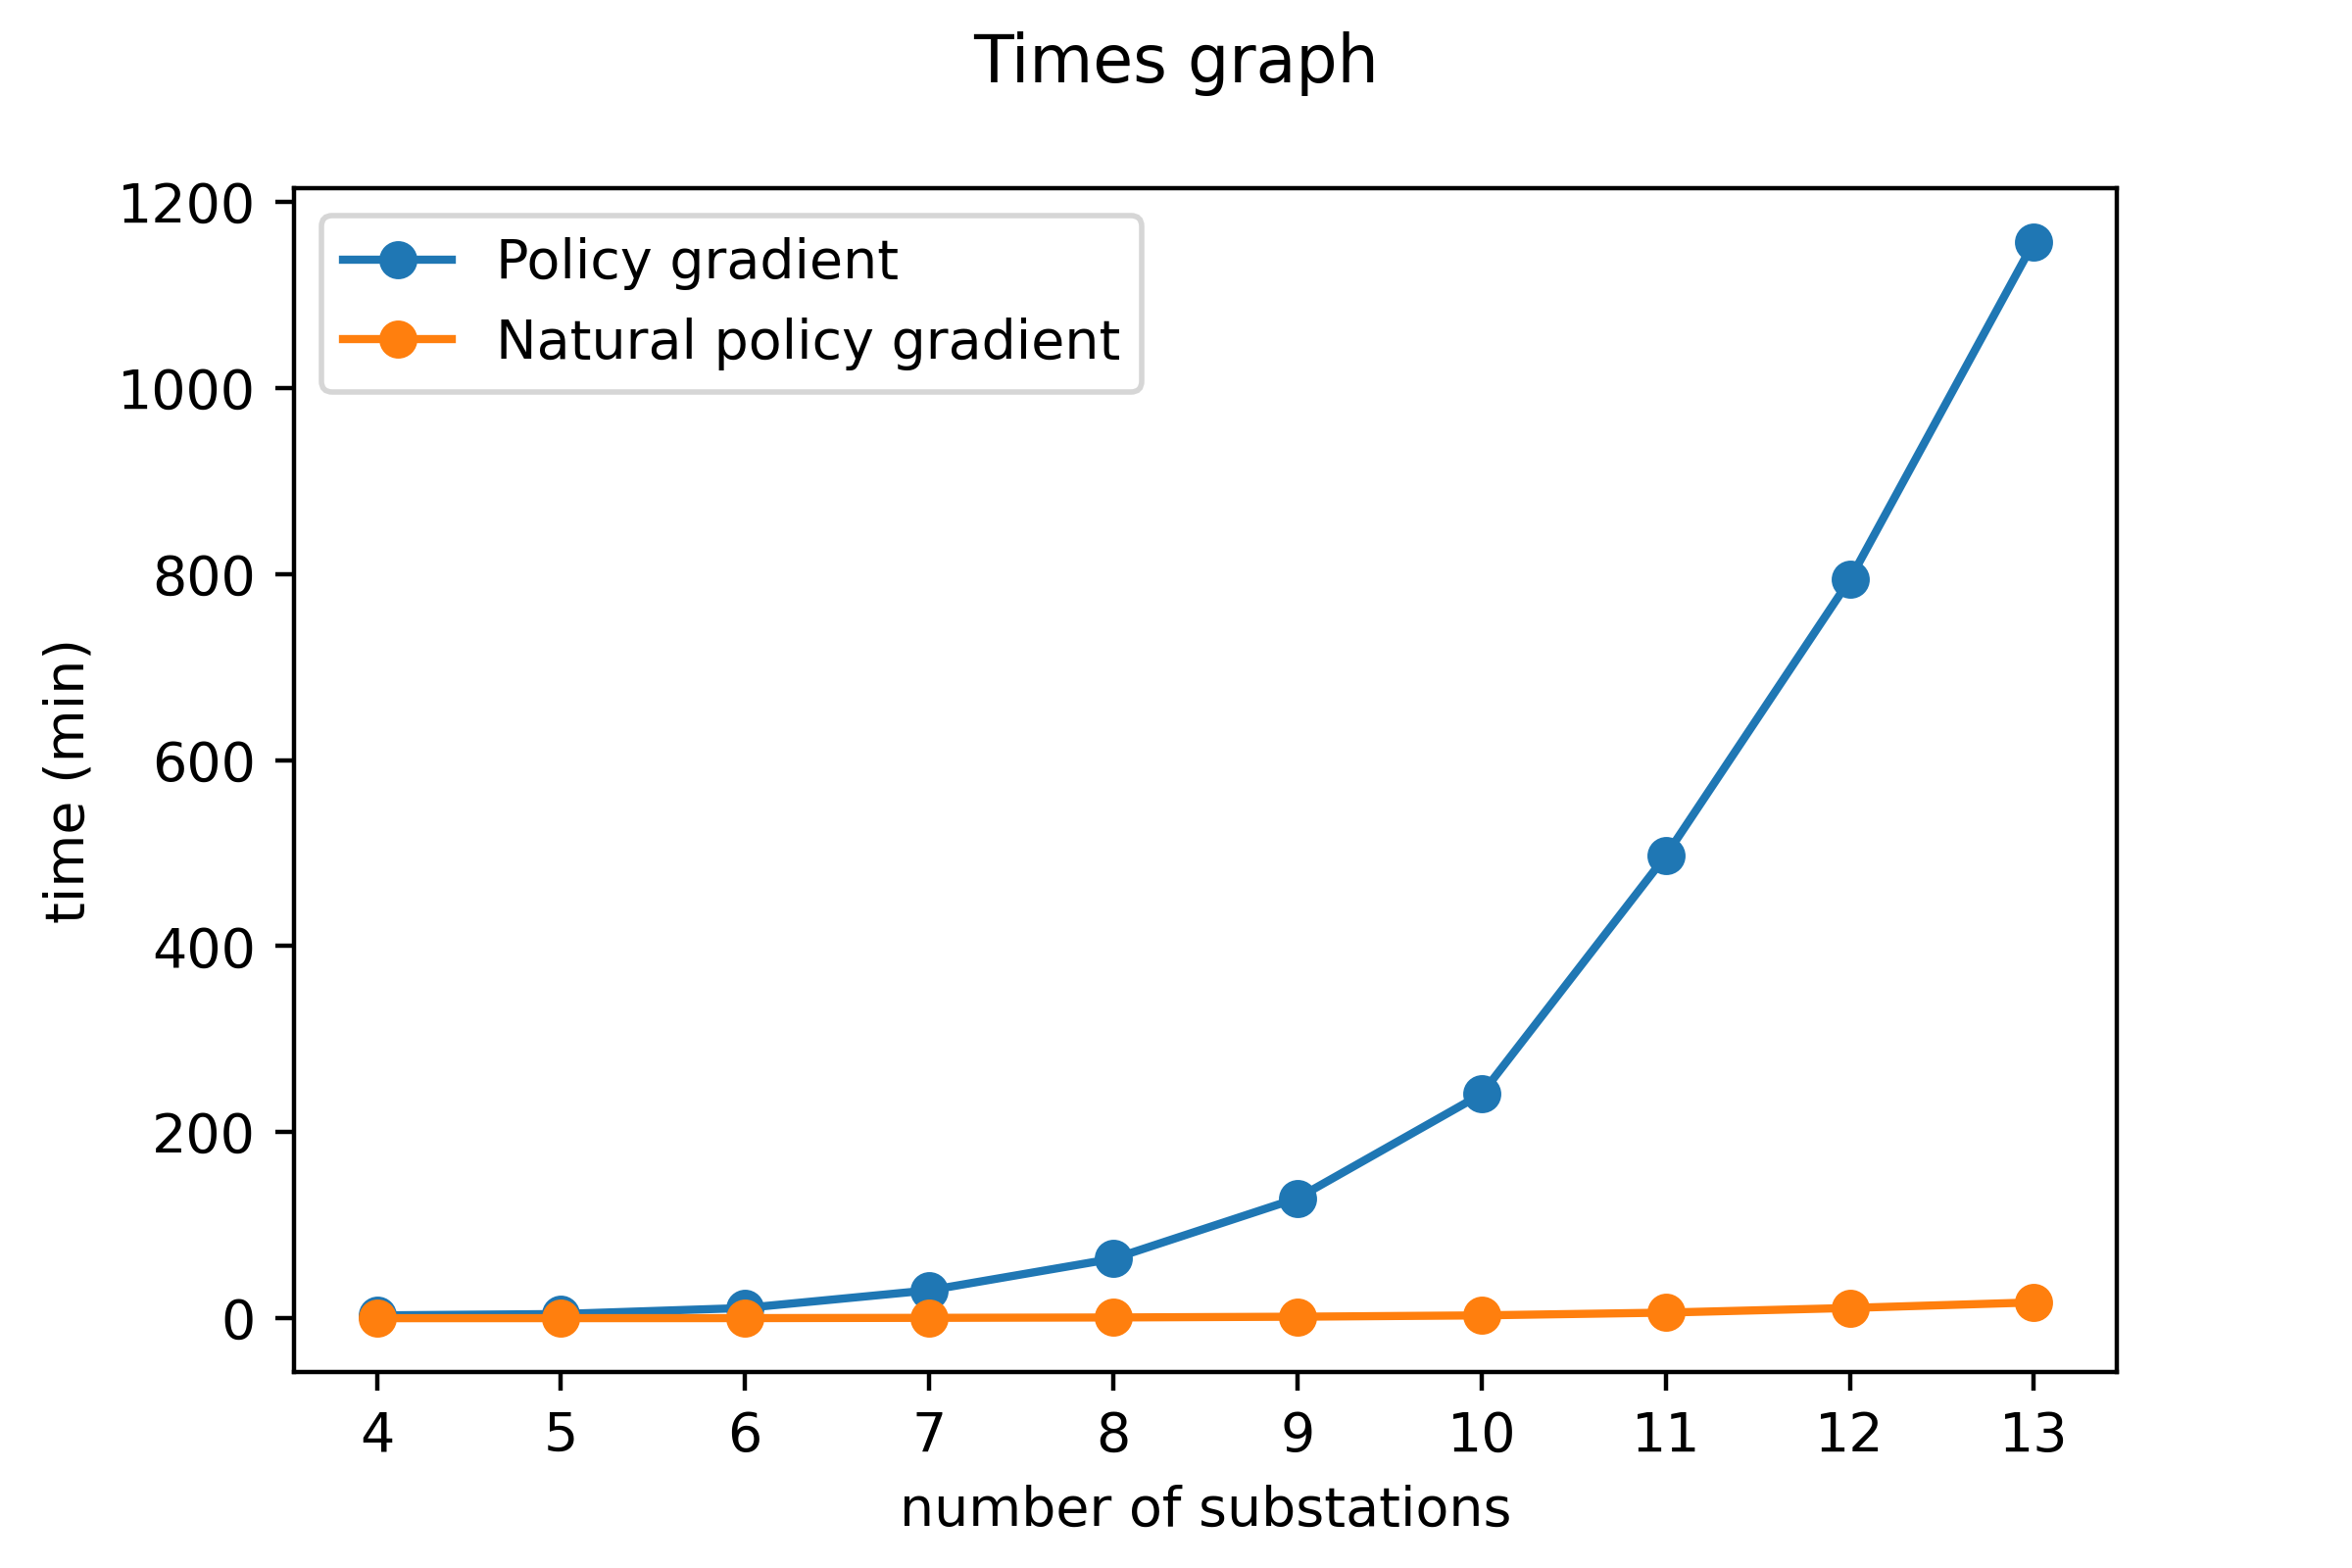
\includegraphics[width=0.55\textwidth]{chapters/figures/times_graph.png}
        \hspace*{-19.5pt}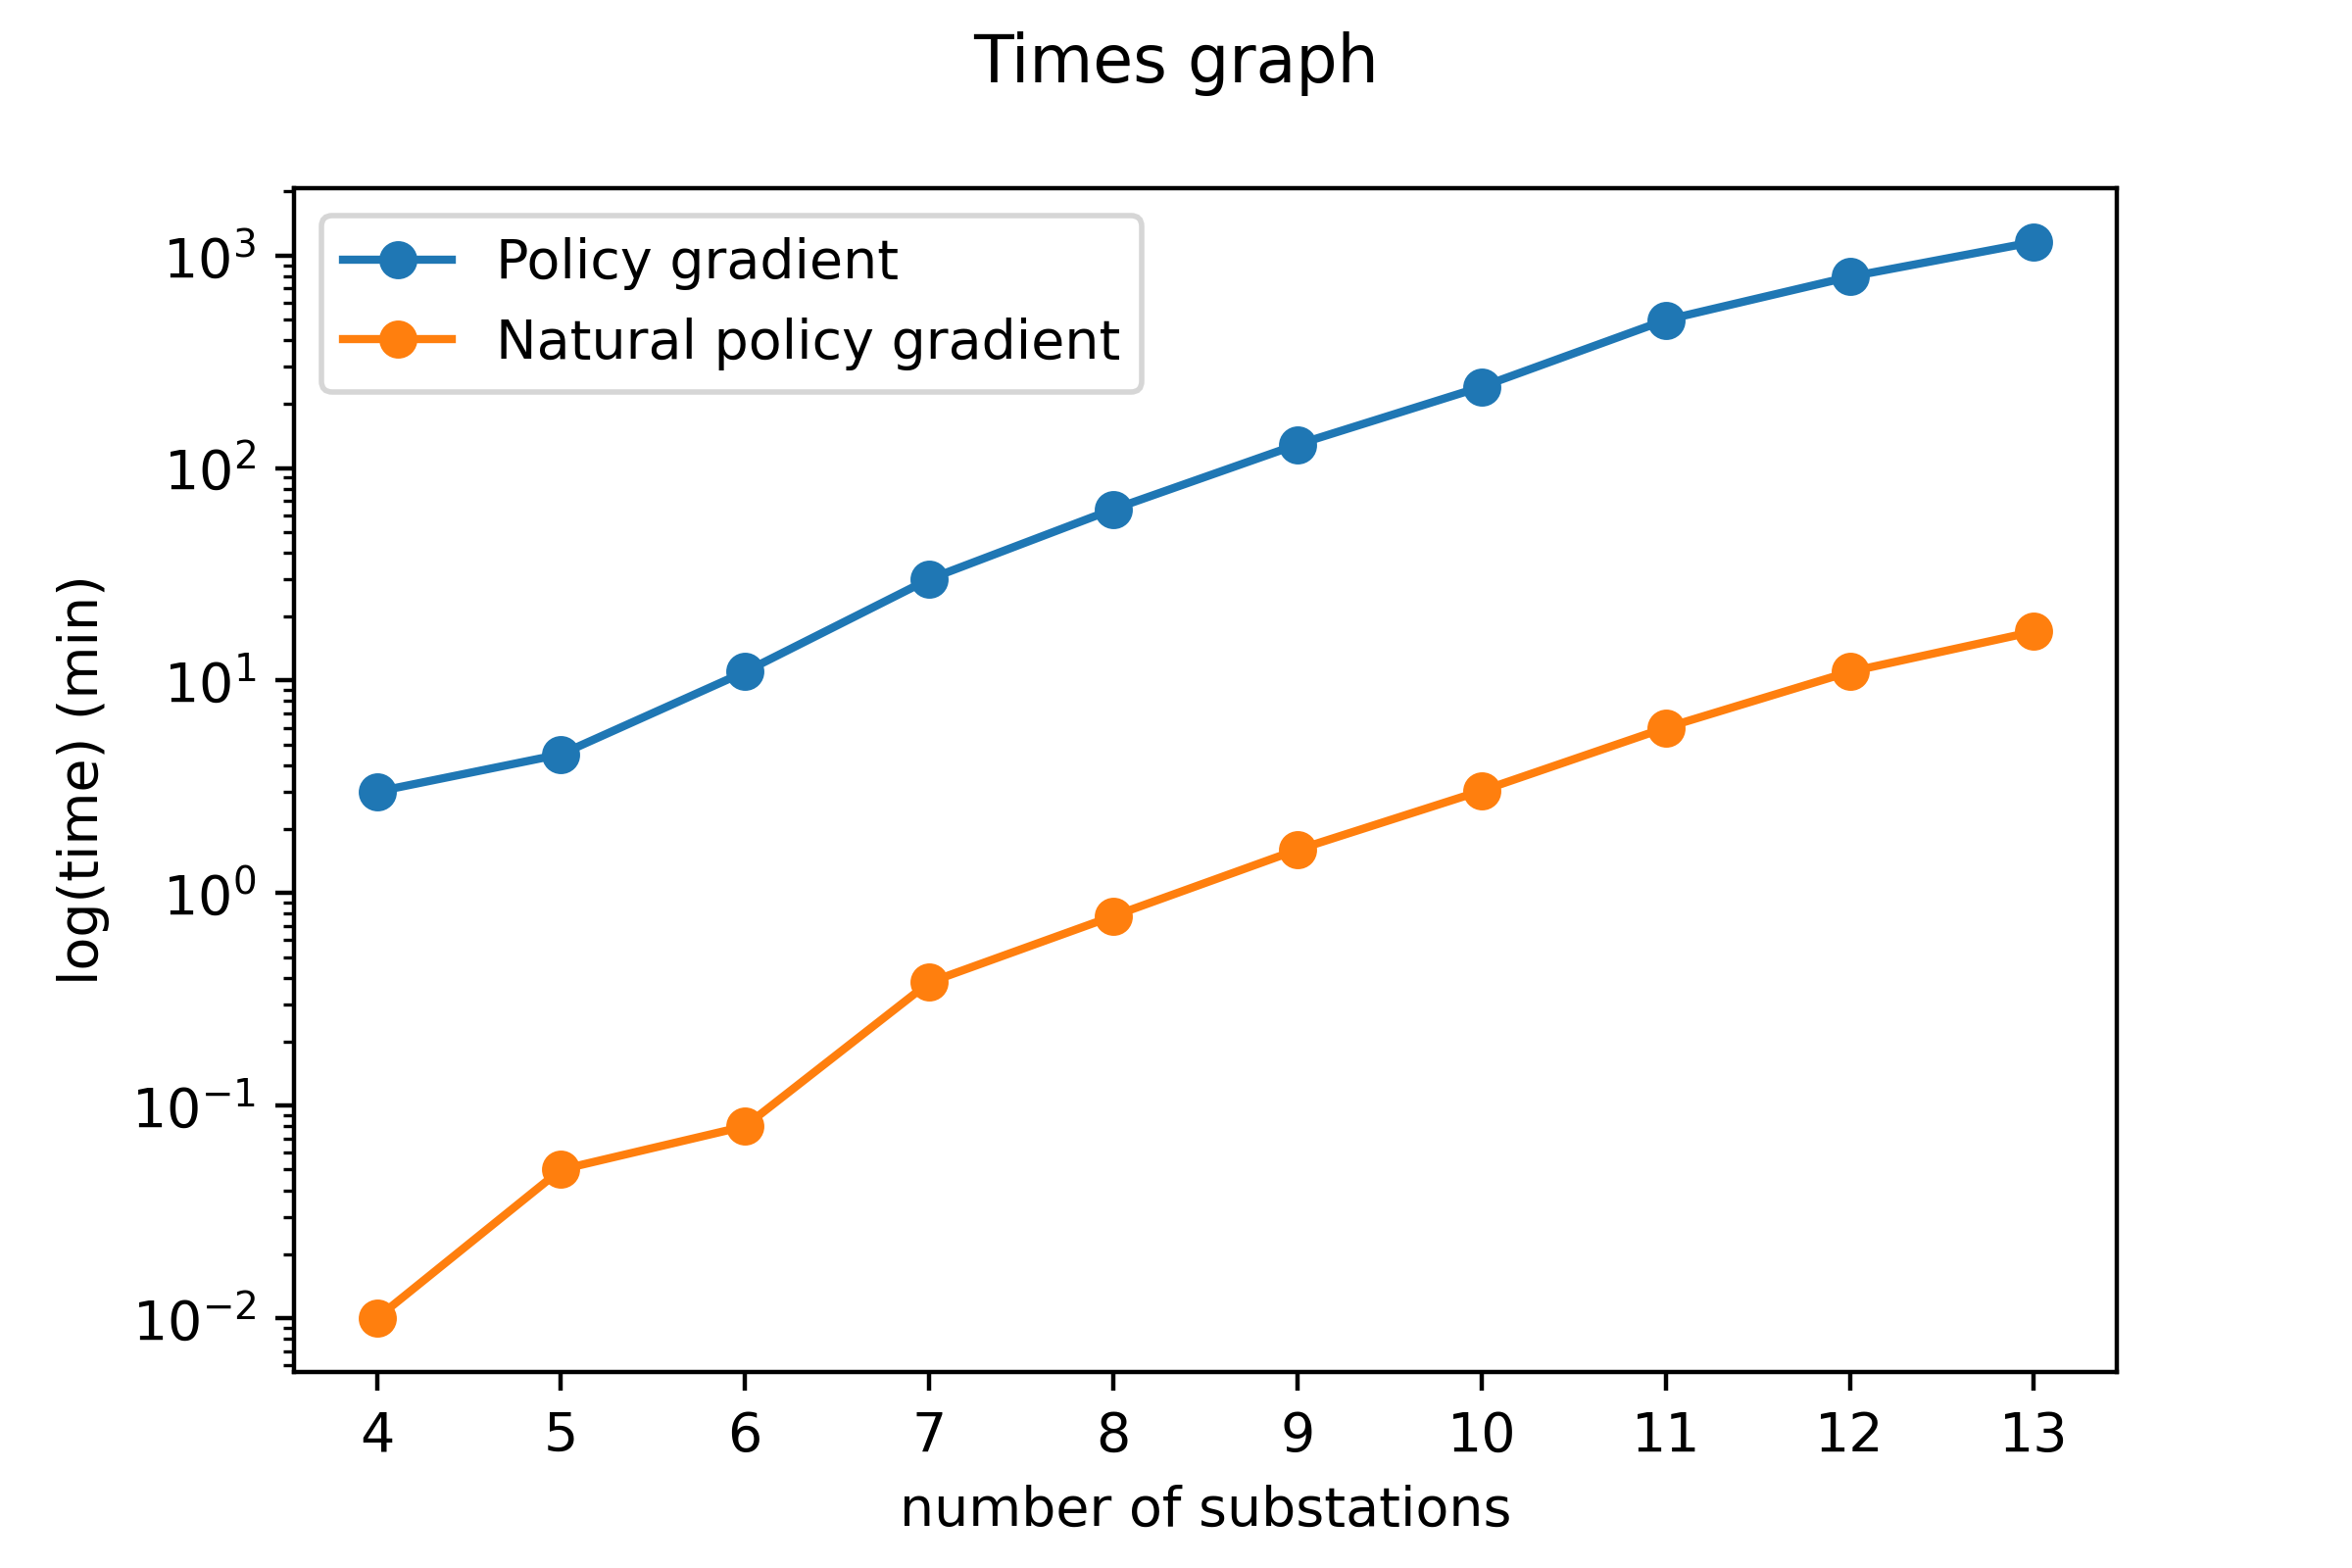
\includegraphics[width=0.55\textwidth]{chapters/figures/times_graph_log.png}
    }
    \caption{Comparison of the times of \acrshort{pg} and \acrshort{npg}. The second figure shows the same times in logarithmic scale.}
    \label{fig:times}
\end{figure}

The first thing to look at in a policy gradient algorithm is whether the gradient descent reached convergence. The first, immediate, check is to see if the error is decreasing. We checked this both for the \acrshort{pg} algorithm and for the \acrshort{npg} algorithm, and both of them were decreasing. In figure \autoref{fig:errors-pg} we can see the plots of the errors for the ordinary policy gradient: in the left panel there is the complete sequence, while in the right panel we zoomed since the error is less than $1$. In figure \autoref{fig:errors-npg} we can see the two plots for the natural policy gradient.

\begin{figure}[htb]
    \centering
    \mbox{
        \hspace*{-19.5pt}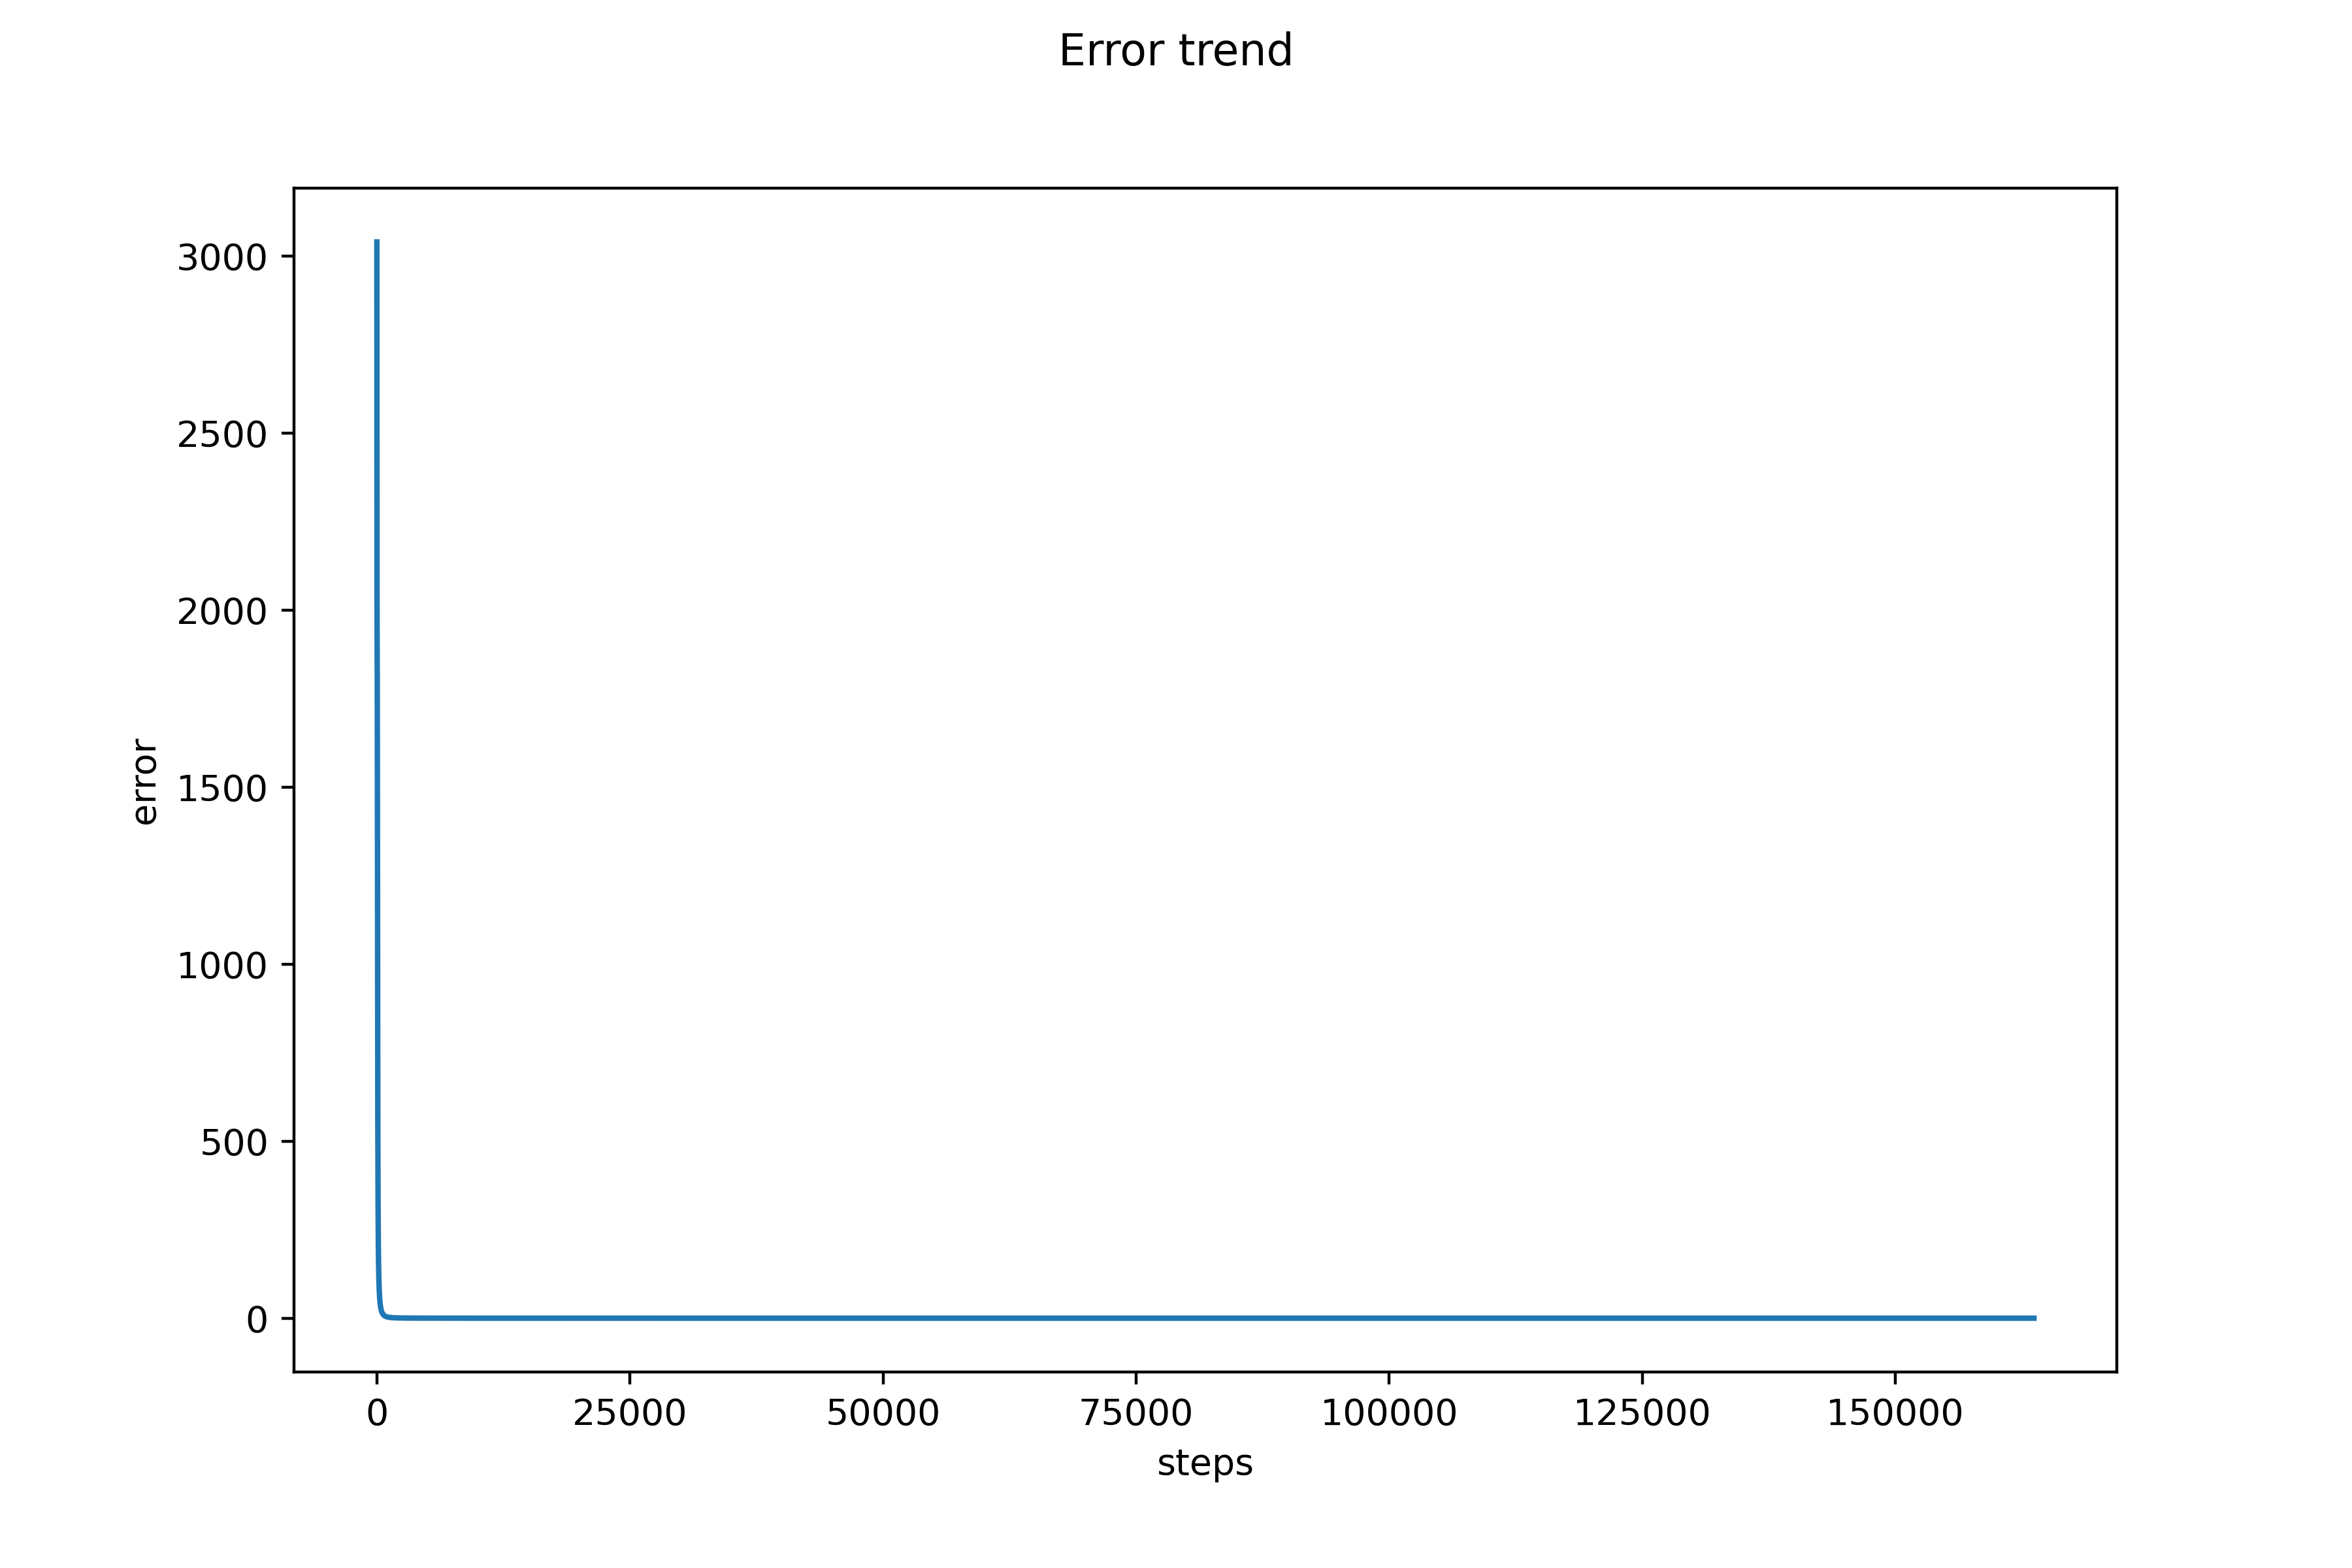
\includegraphics[width=0.55\textwidth]{chapters/figures/errors_PG.png}
        \hspace*{-15pt}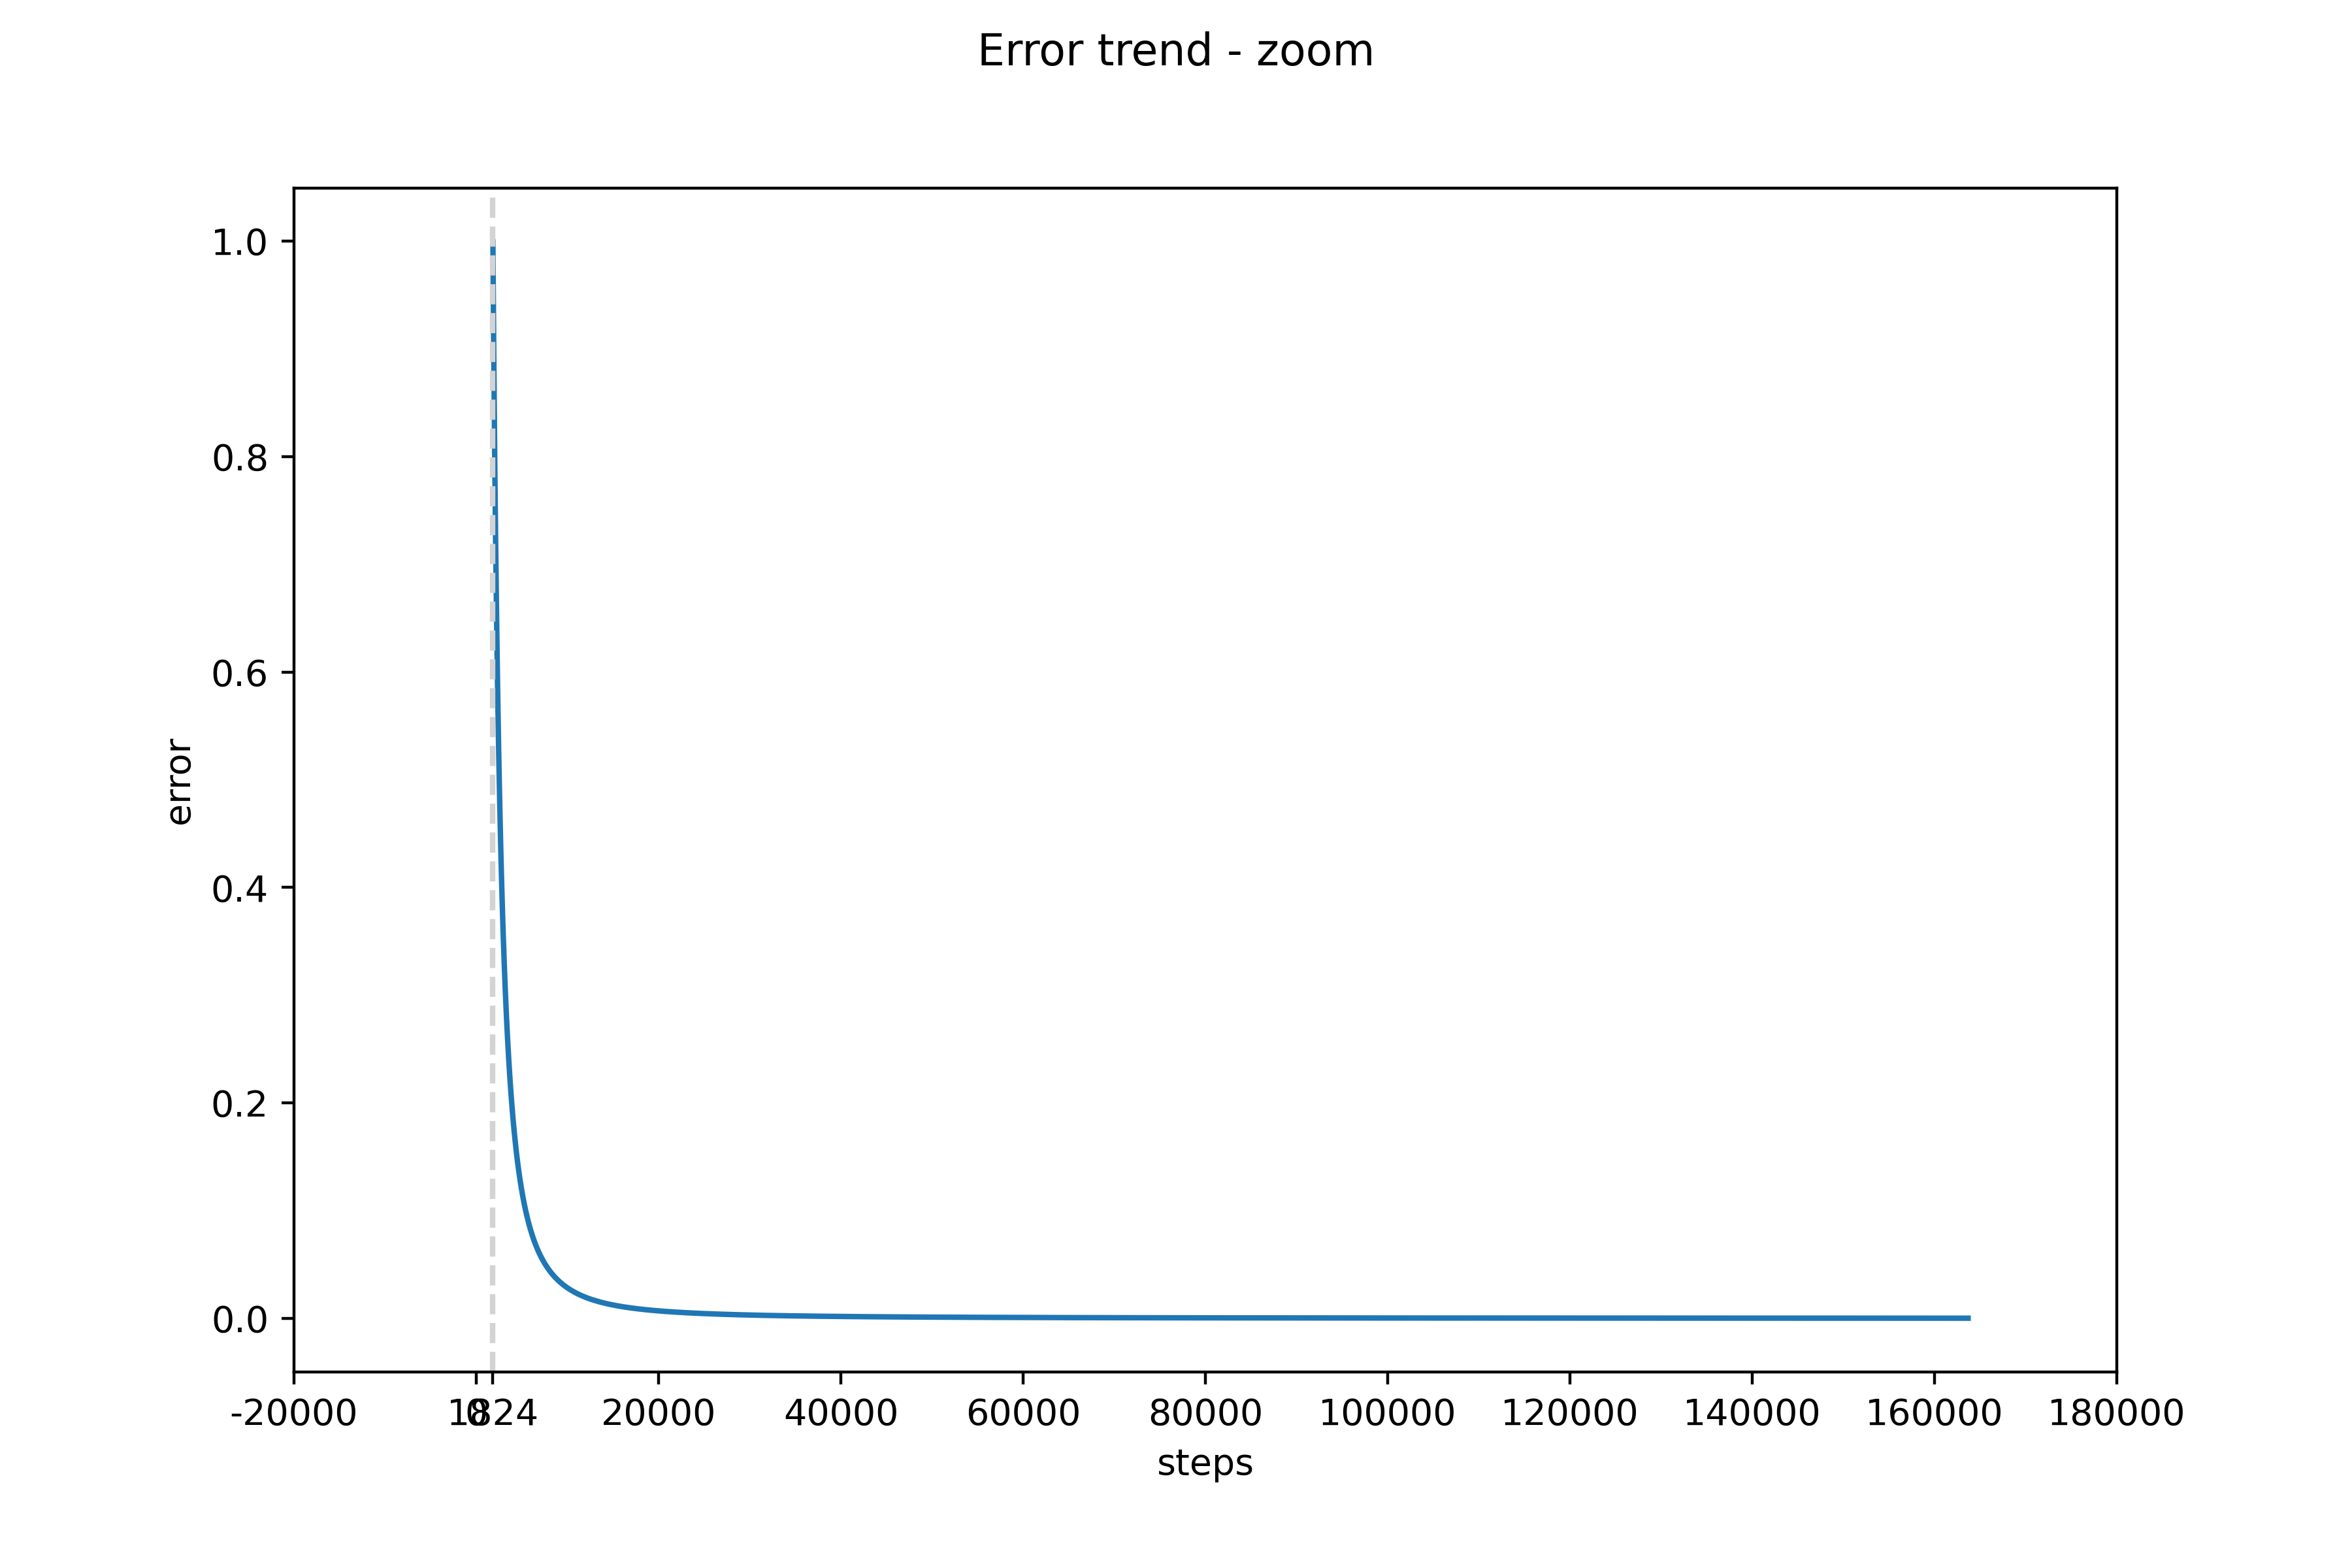
\includegraphics[width=0.55\textwidth]{chapters/figures/errors_zoom_PG.png}
    }
    \caption{\acrshort{pg} errors: they are decreasing, like they should.}
    \label{fig:errors-pg}
\end{figure}

\begin{figure}[htb]
    \centering
    \mbox{
        \hspace*{-19.5pt}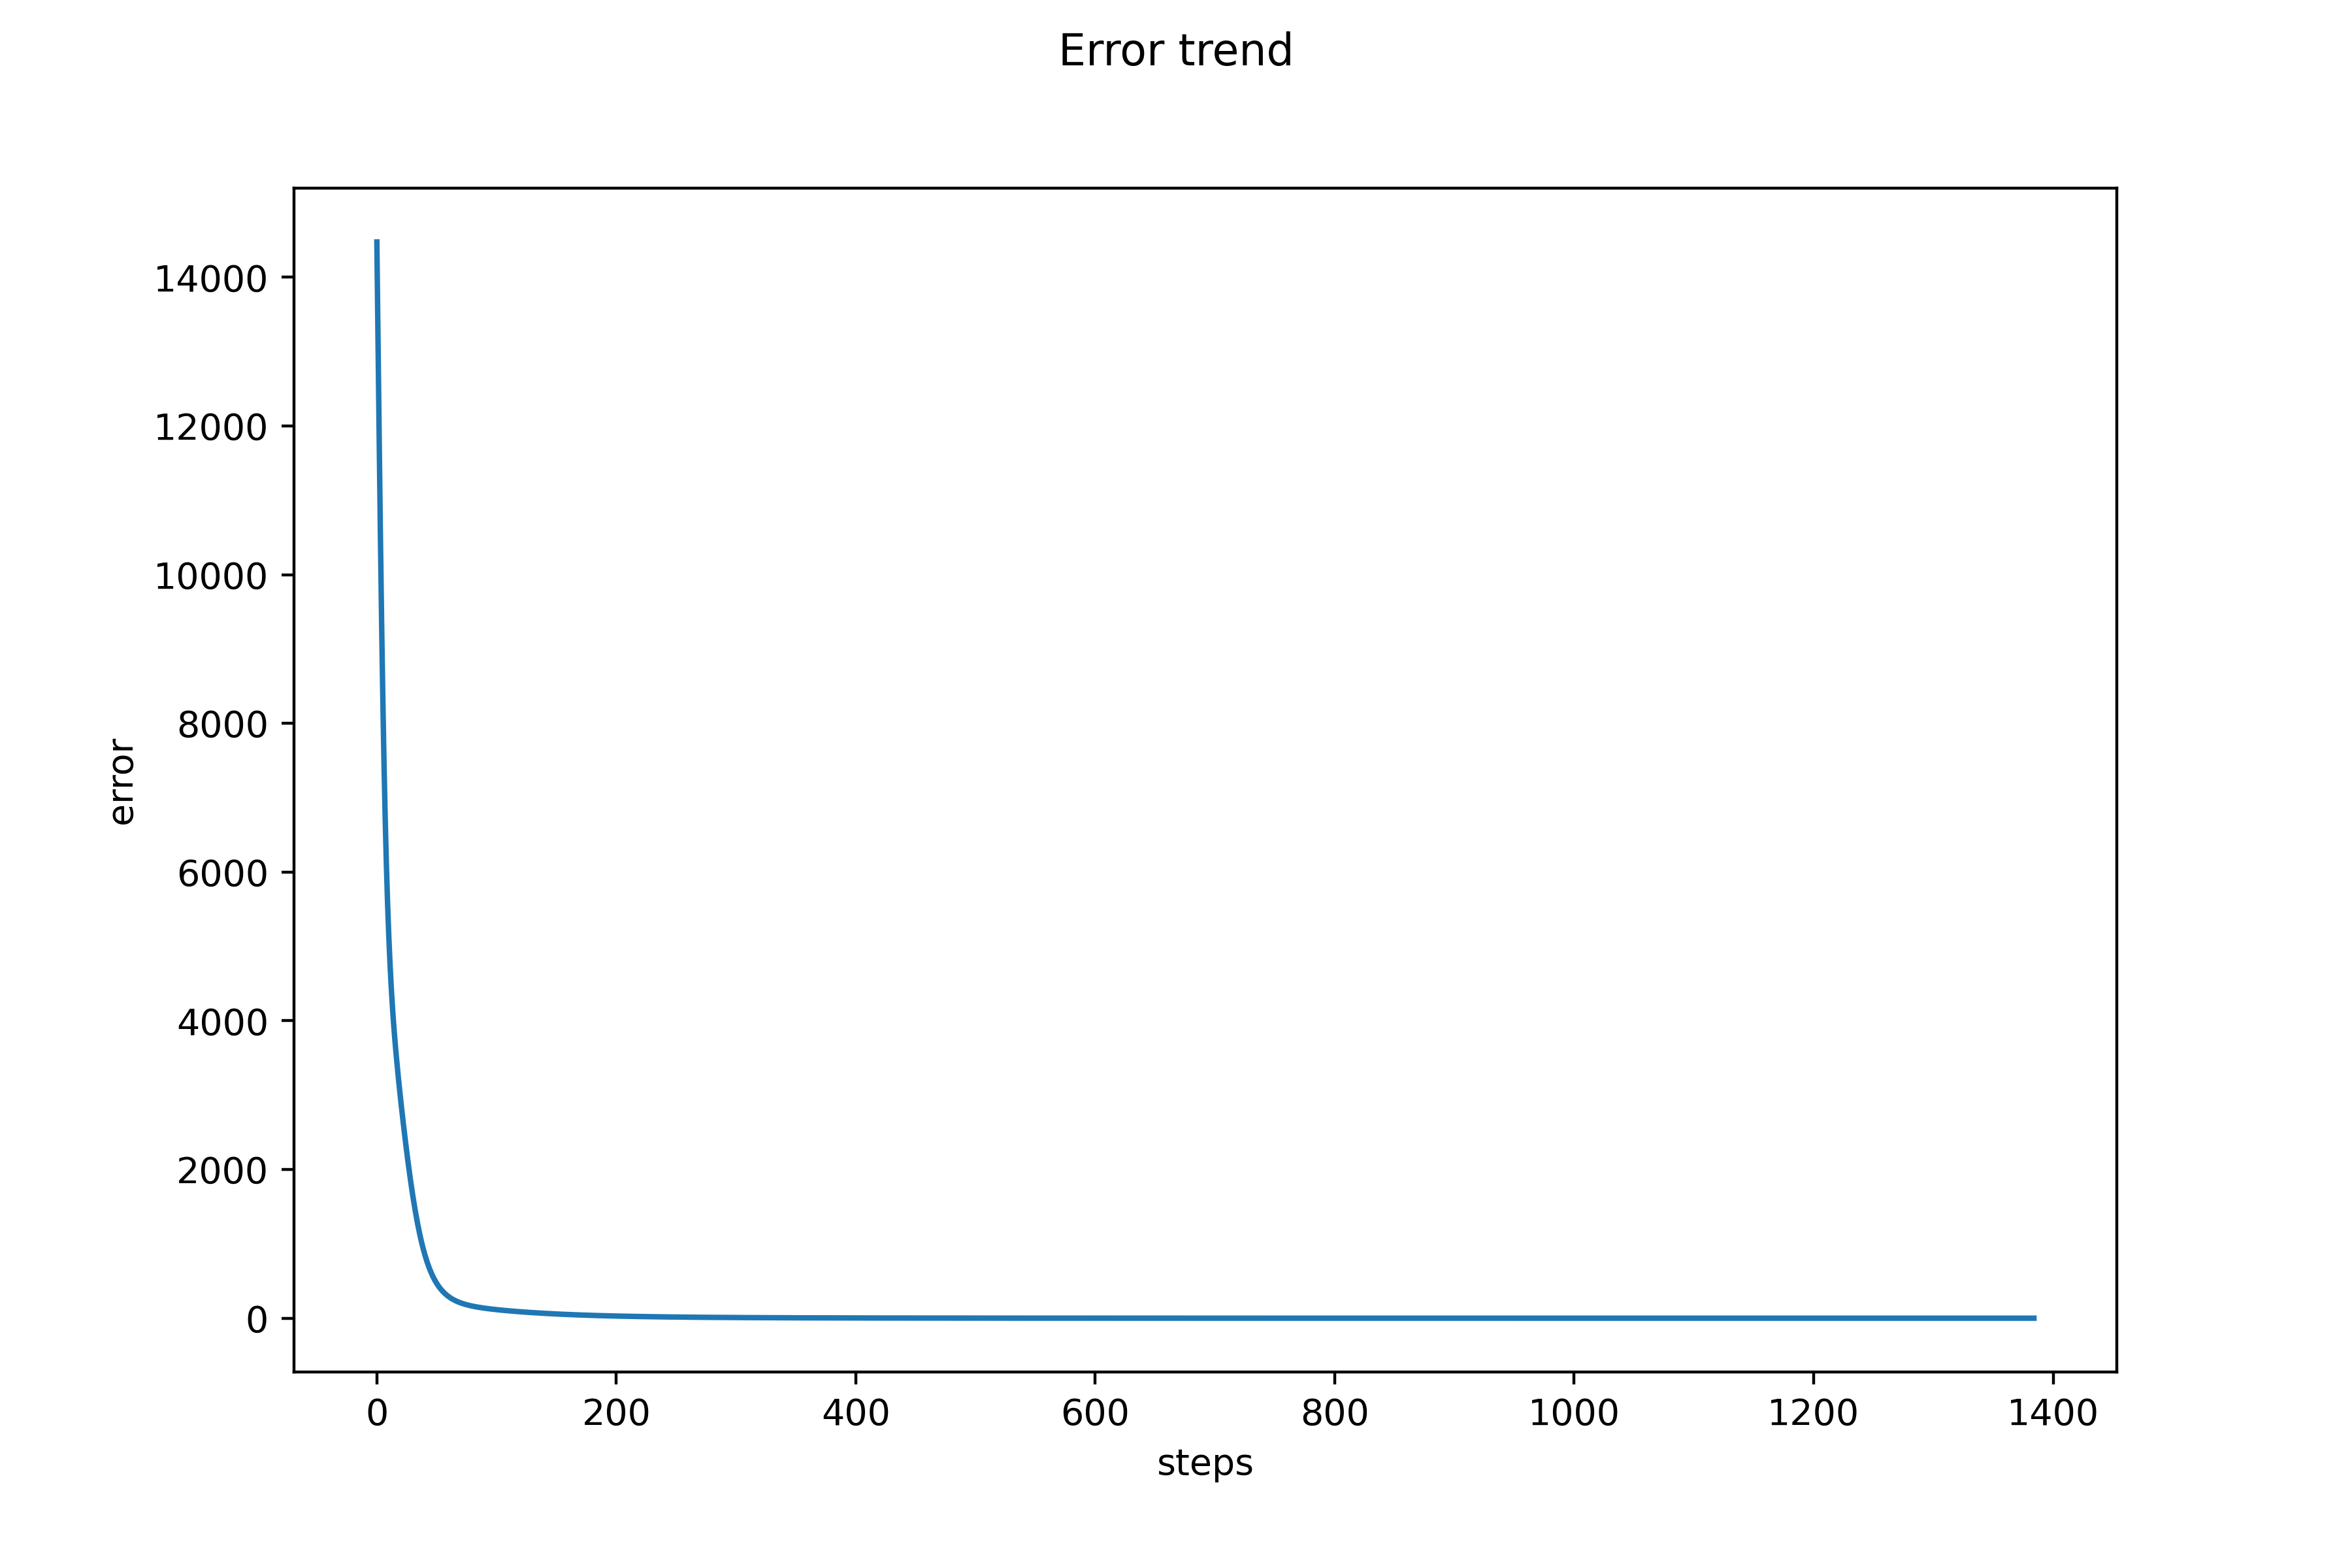
\includegraphics[width=0.55\textwidth]{chapters/figures/errors_NPG.png}
        \hspace*{-15pt}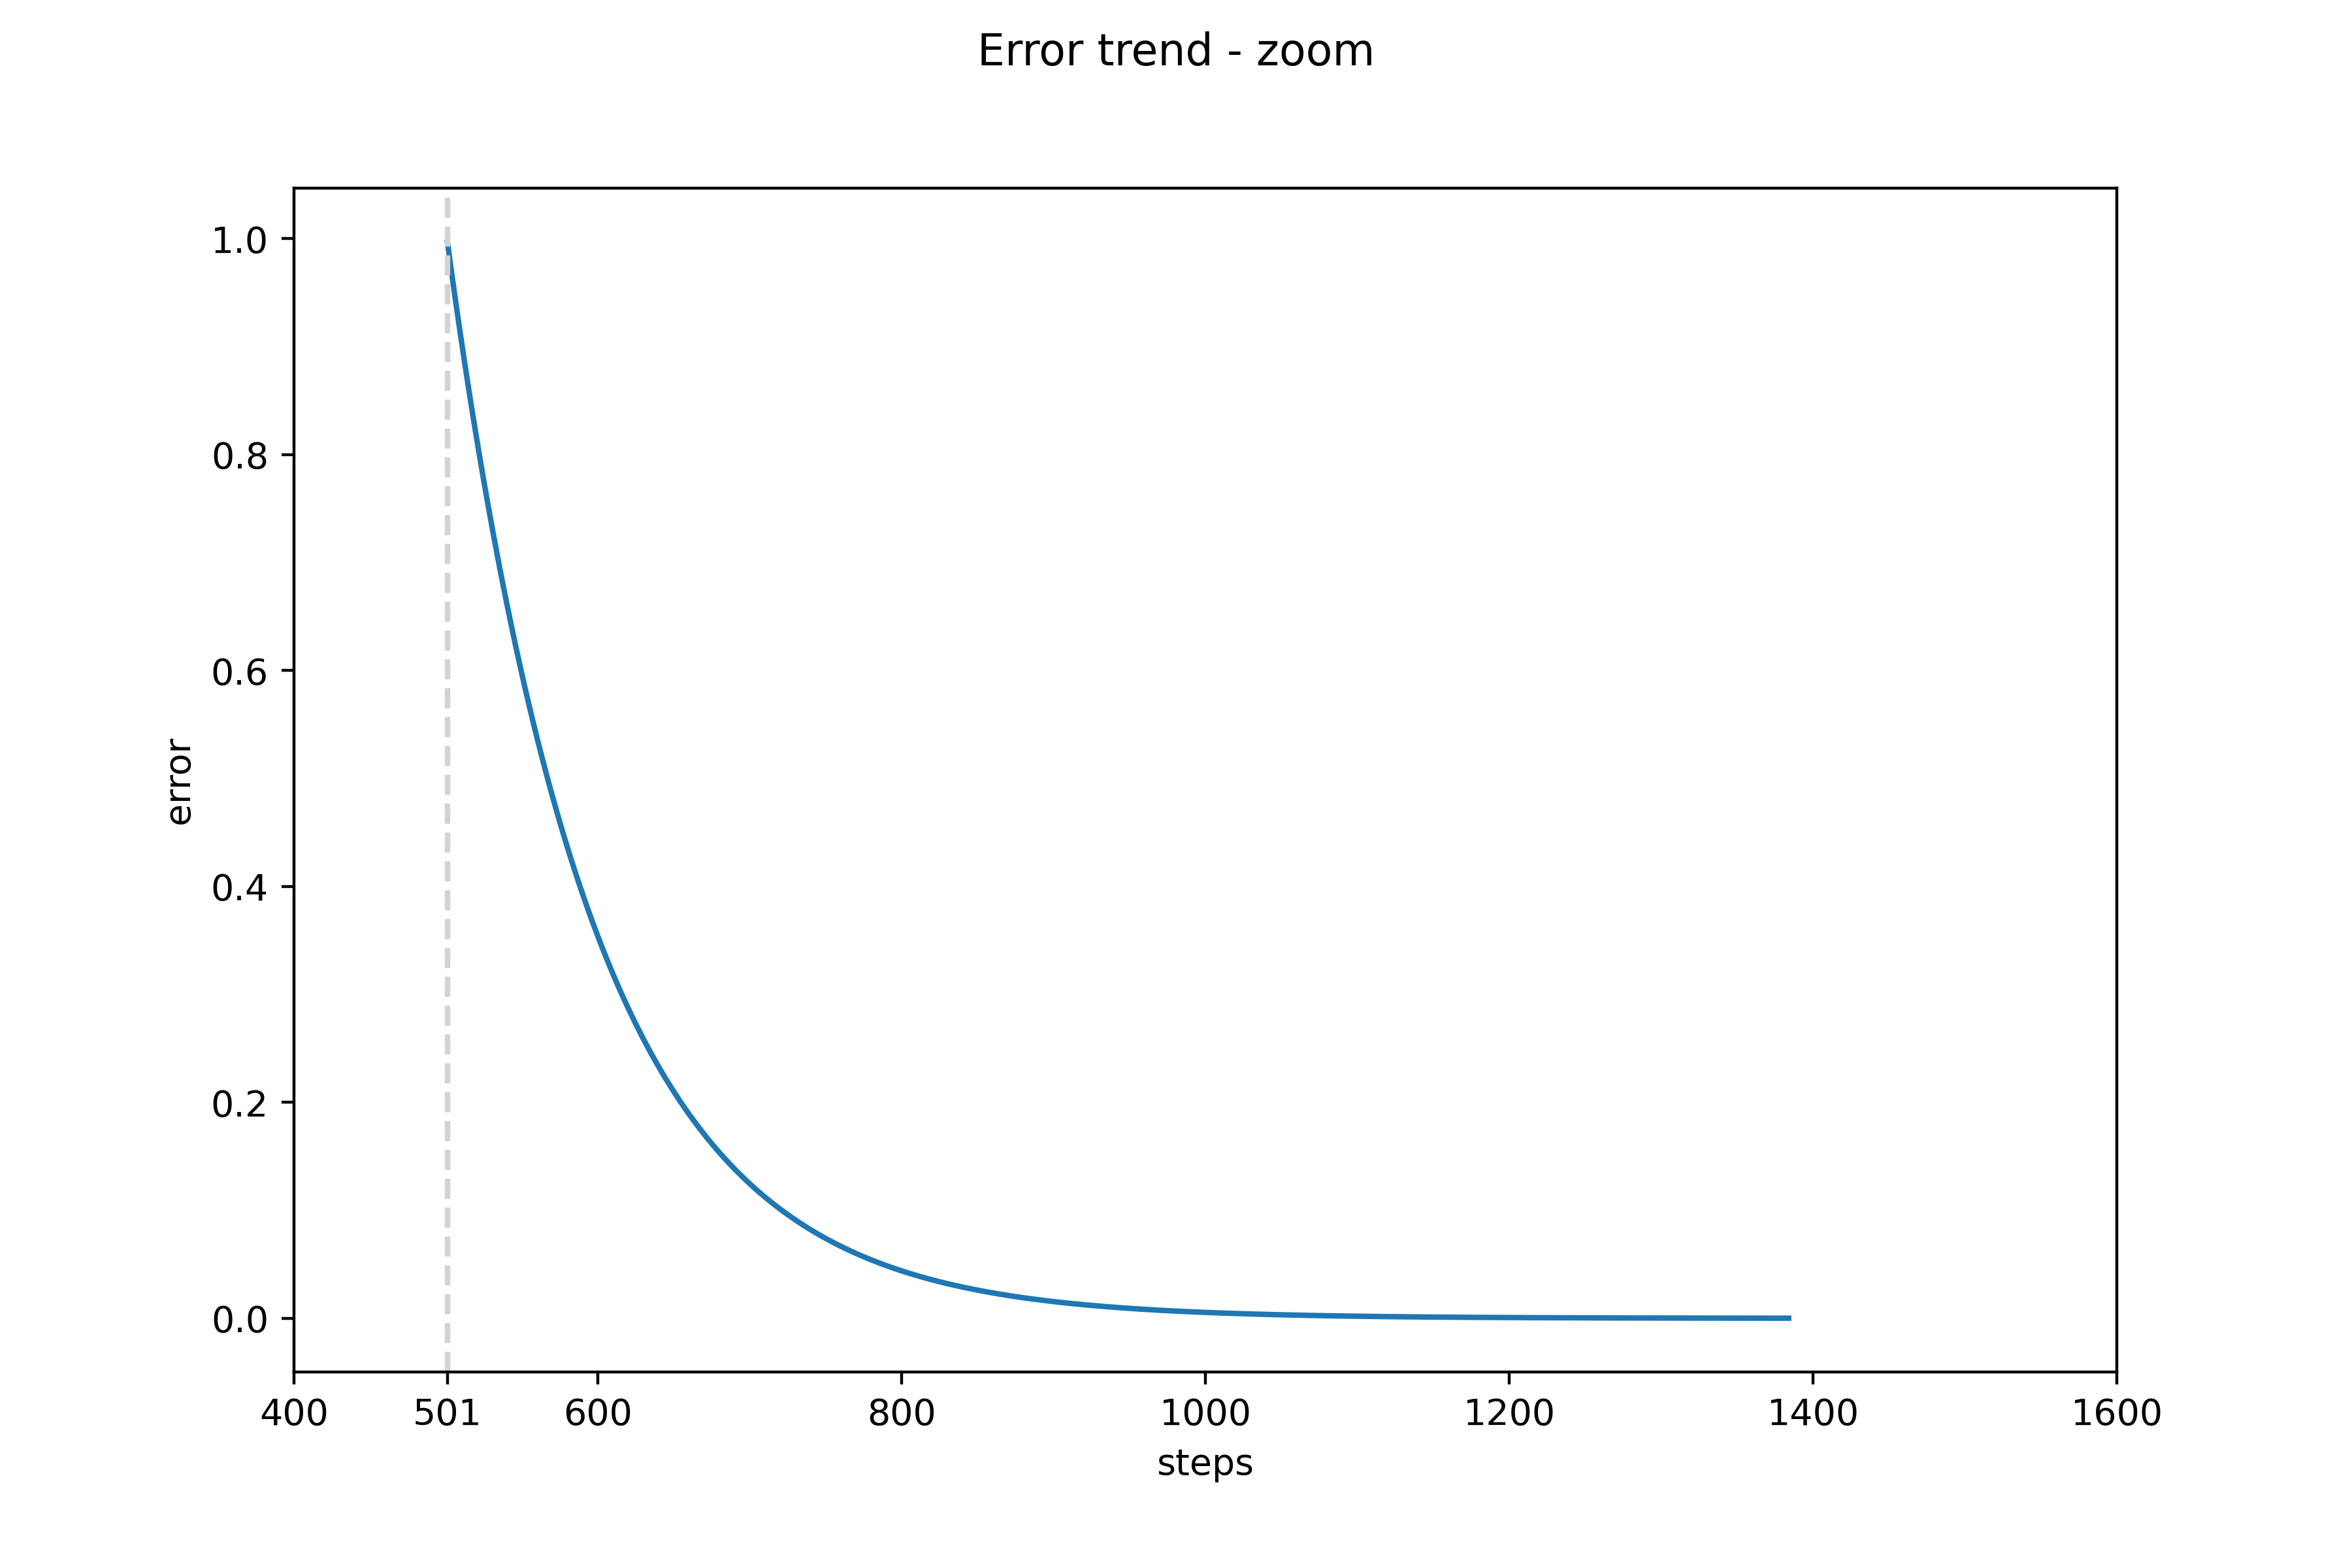
\includegraphics[width=0.55\textwidth]{chapters/figures/errors_zoom_NPG.png}
    }
    \caption{\acrshort{npg} errors: they are decreasing, like they should.}
    \label{fig:errors-npg}
\end{figure}

However, this is not enough to say that the algorithm converged, this is a mere indicator that the gradient descent is indeed following the gradient and moving towards a minimum. Thus, what we did next was to examine the trajectories of the parameters $\boldsymbol \theta$ in the parameters space and the trajectories of the policies $\pi_{\boldsymbol \theta}$ in the policy space. In \autoref{fig:sequence-theta-pg} and \autoref{fig:sequence-policies-pg} we can see them for the \acrshort{pg}, where we selected a specific episode with $5$ initially disconnected substation and the fault among the second and the third substation. In \autoref{fig:sequence-theta-npg} and \autoref{fig:sequence-policies-npg} we can see them for the \acrshort{npg} for the same exact episode.

\begin{figure}[!htp]
    \centering
    \begin{tabular}{cc}
        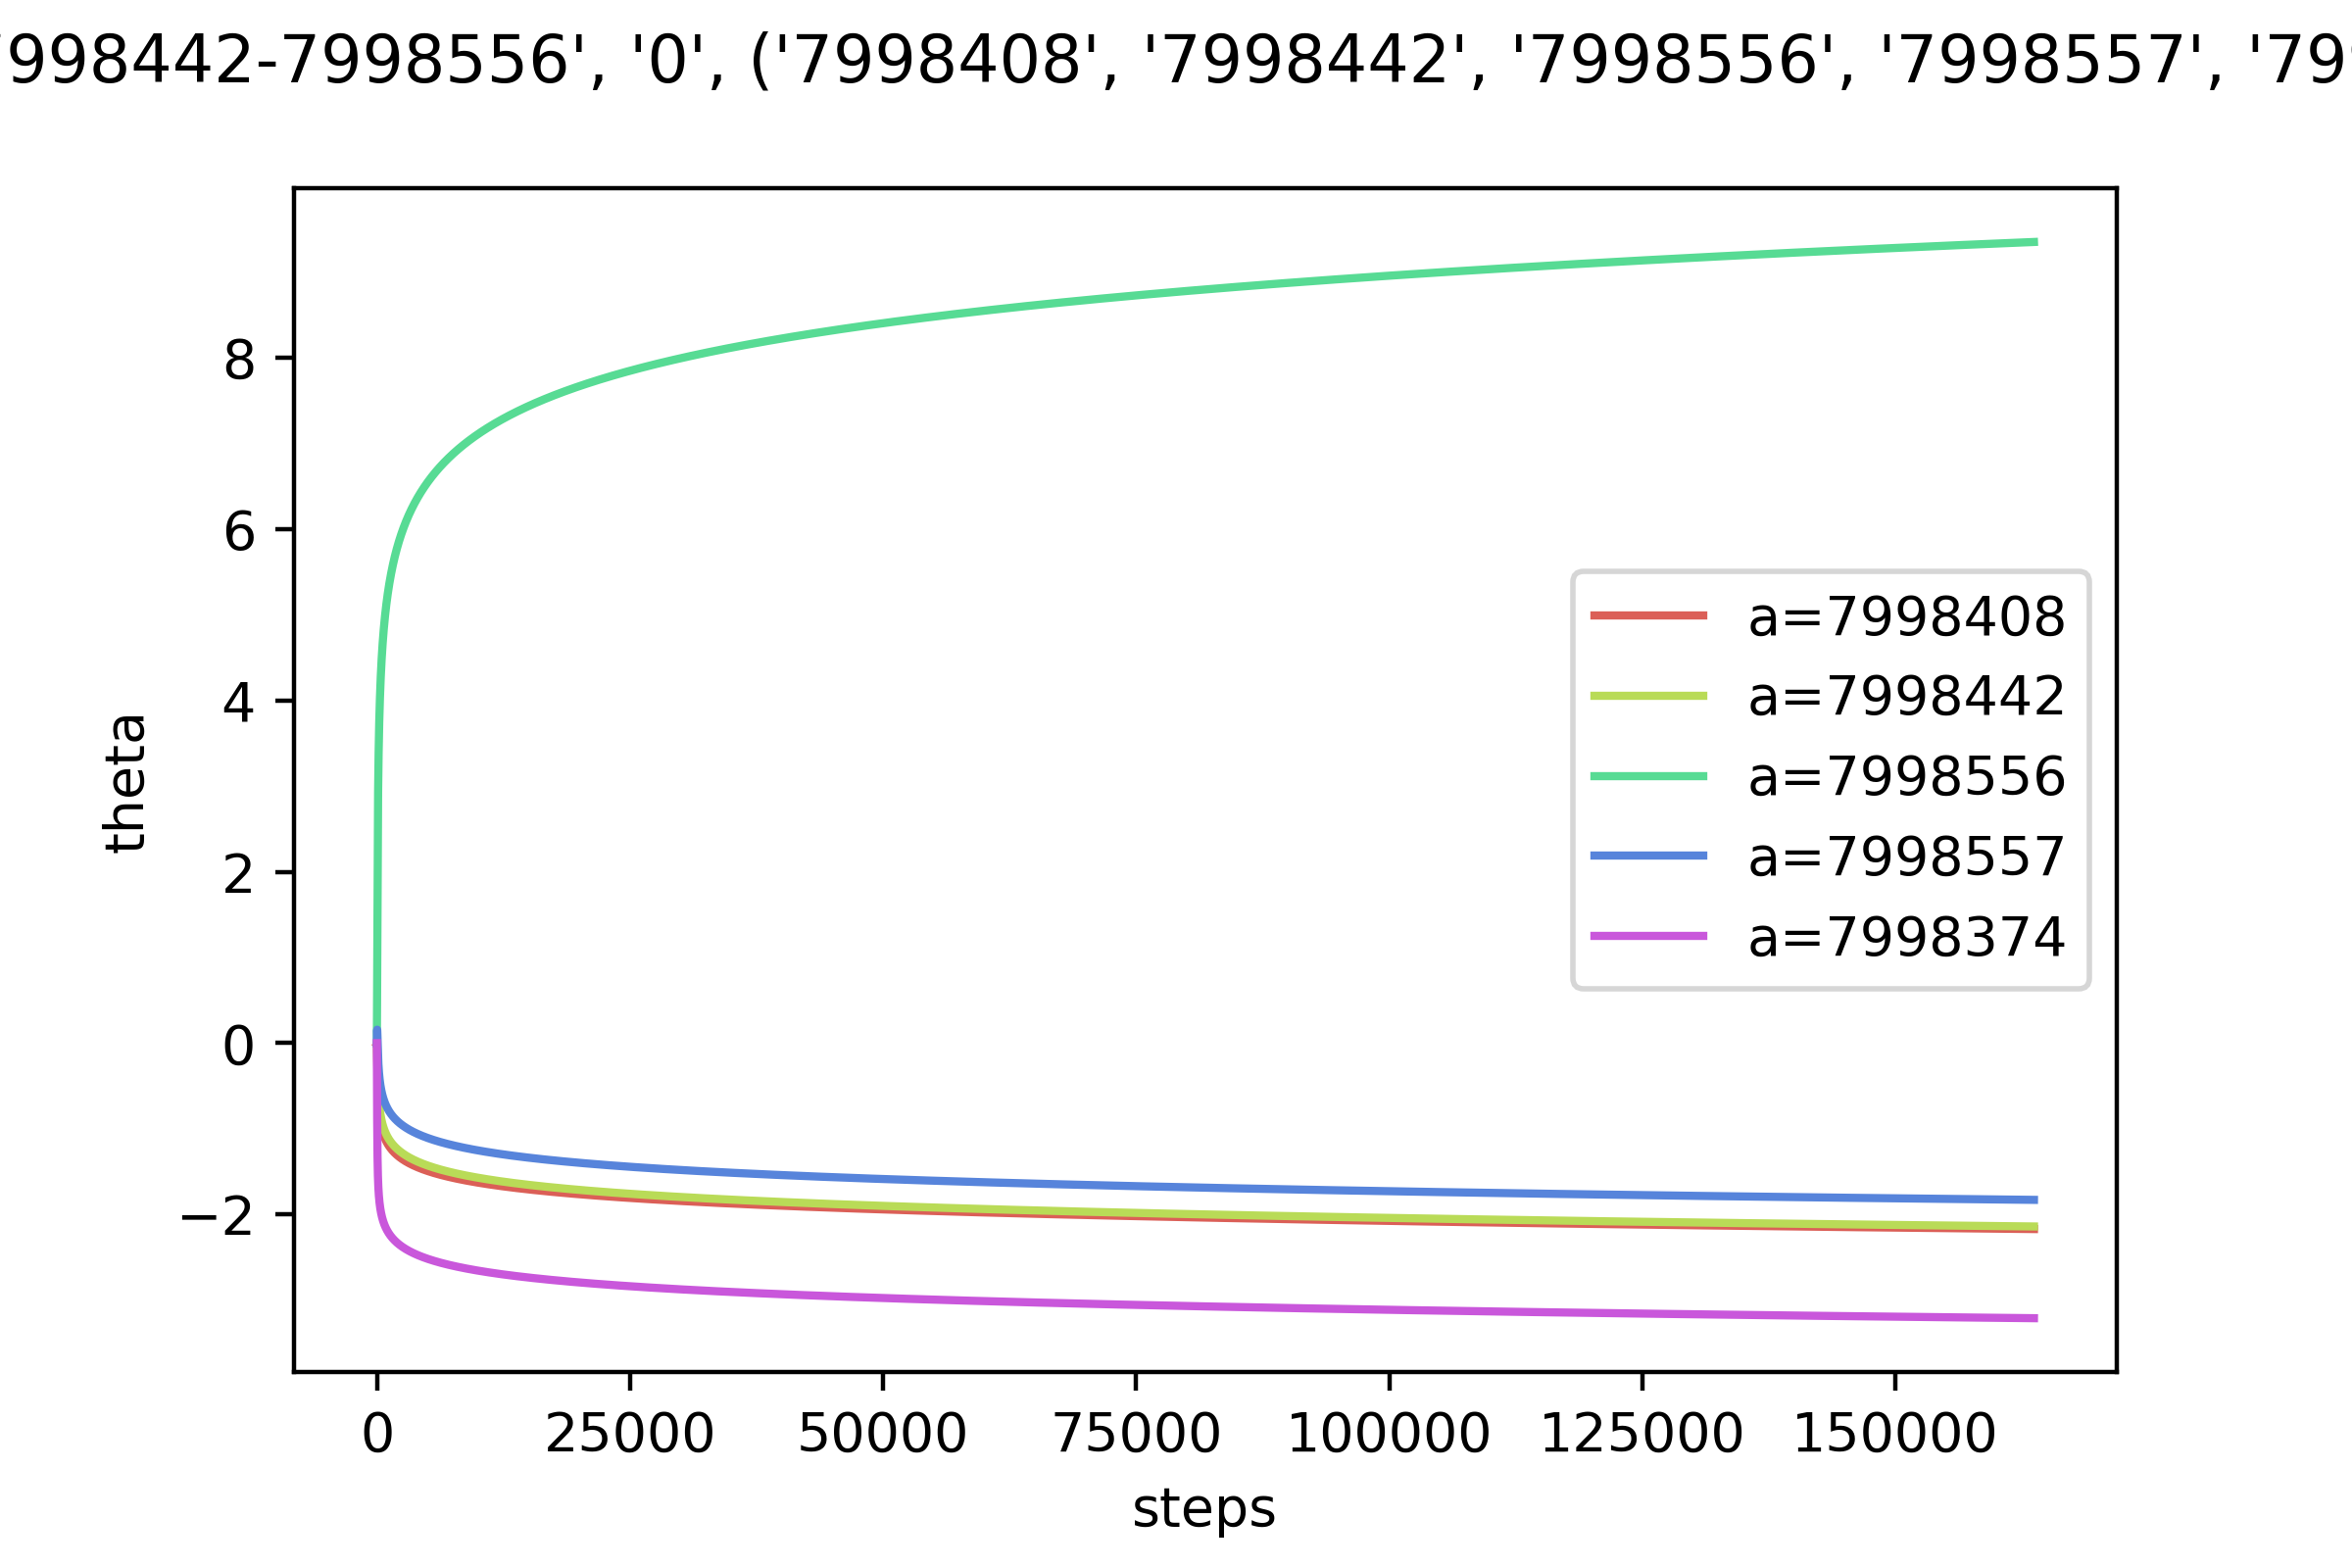
\includegraphics[height=0.27\textwidth,valign=b]{chapters/figures/theta_PG_state_0.png} &
        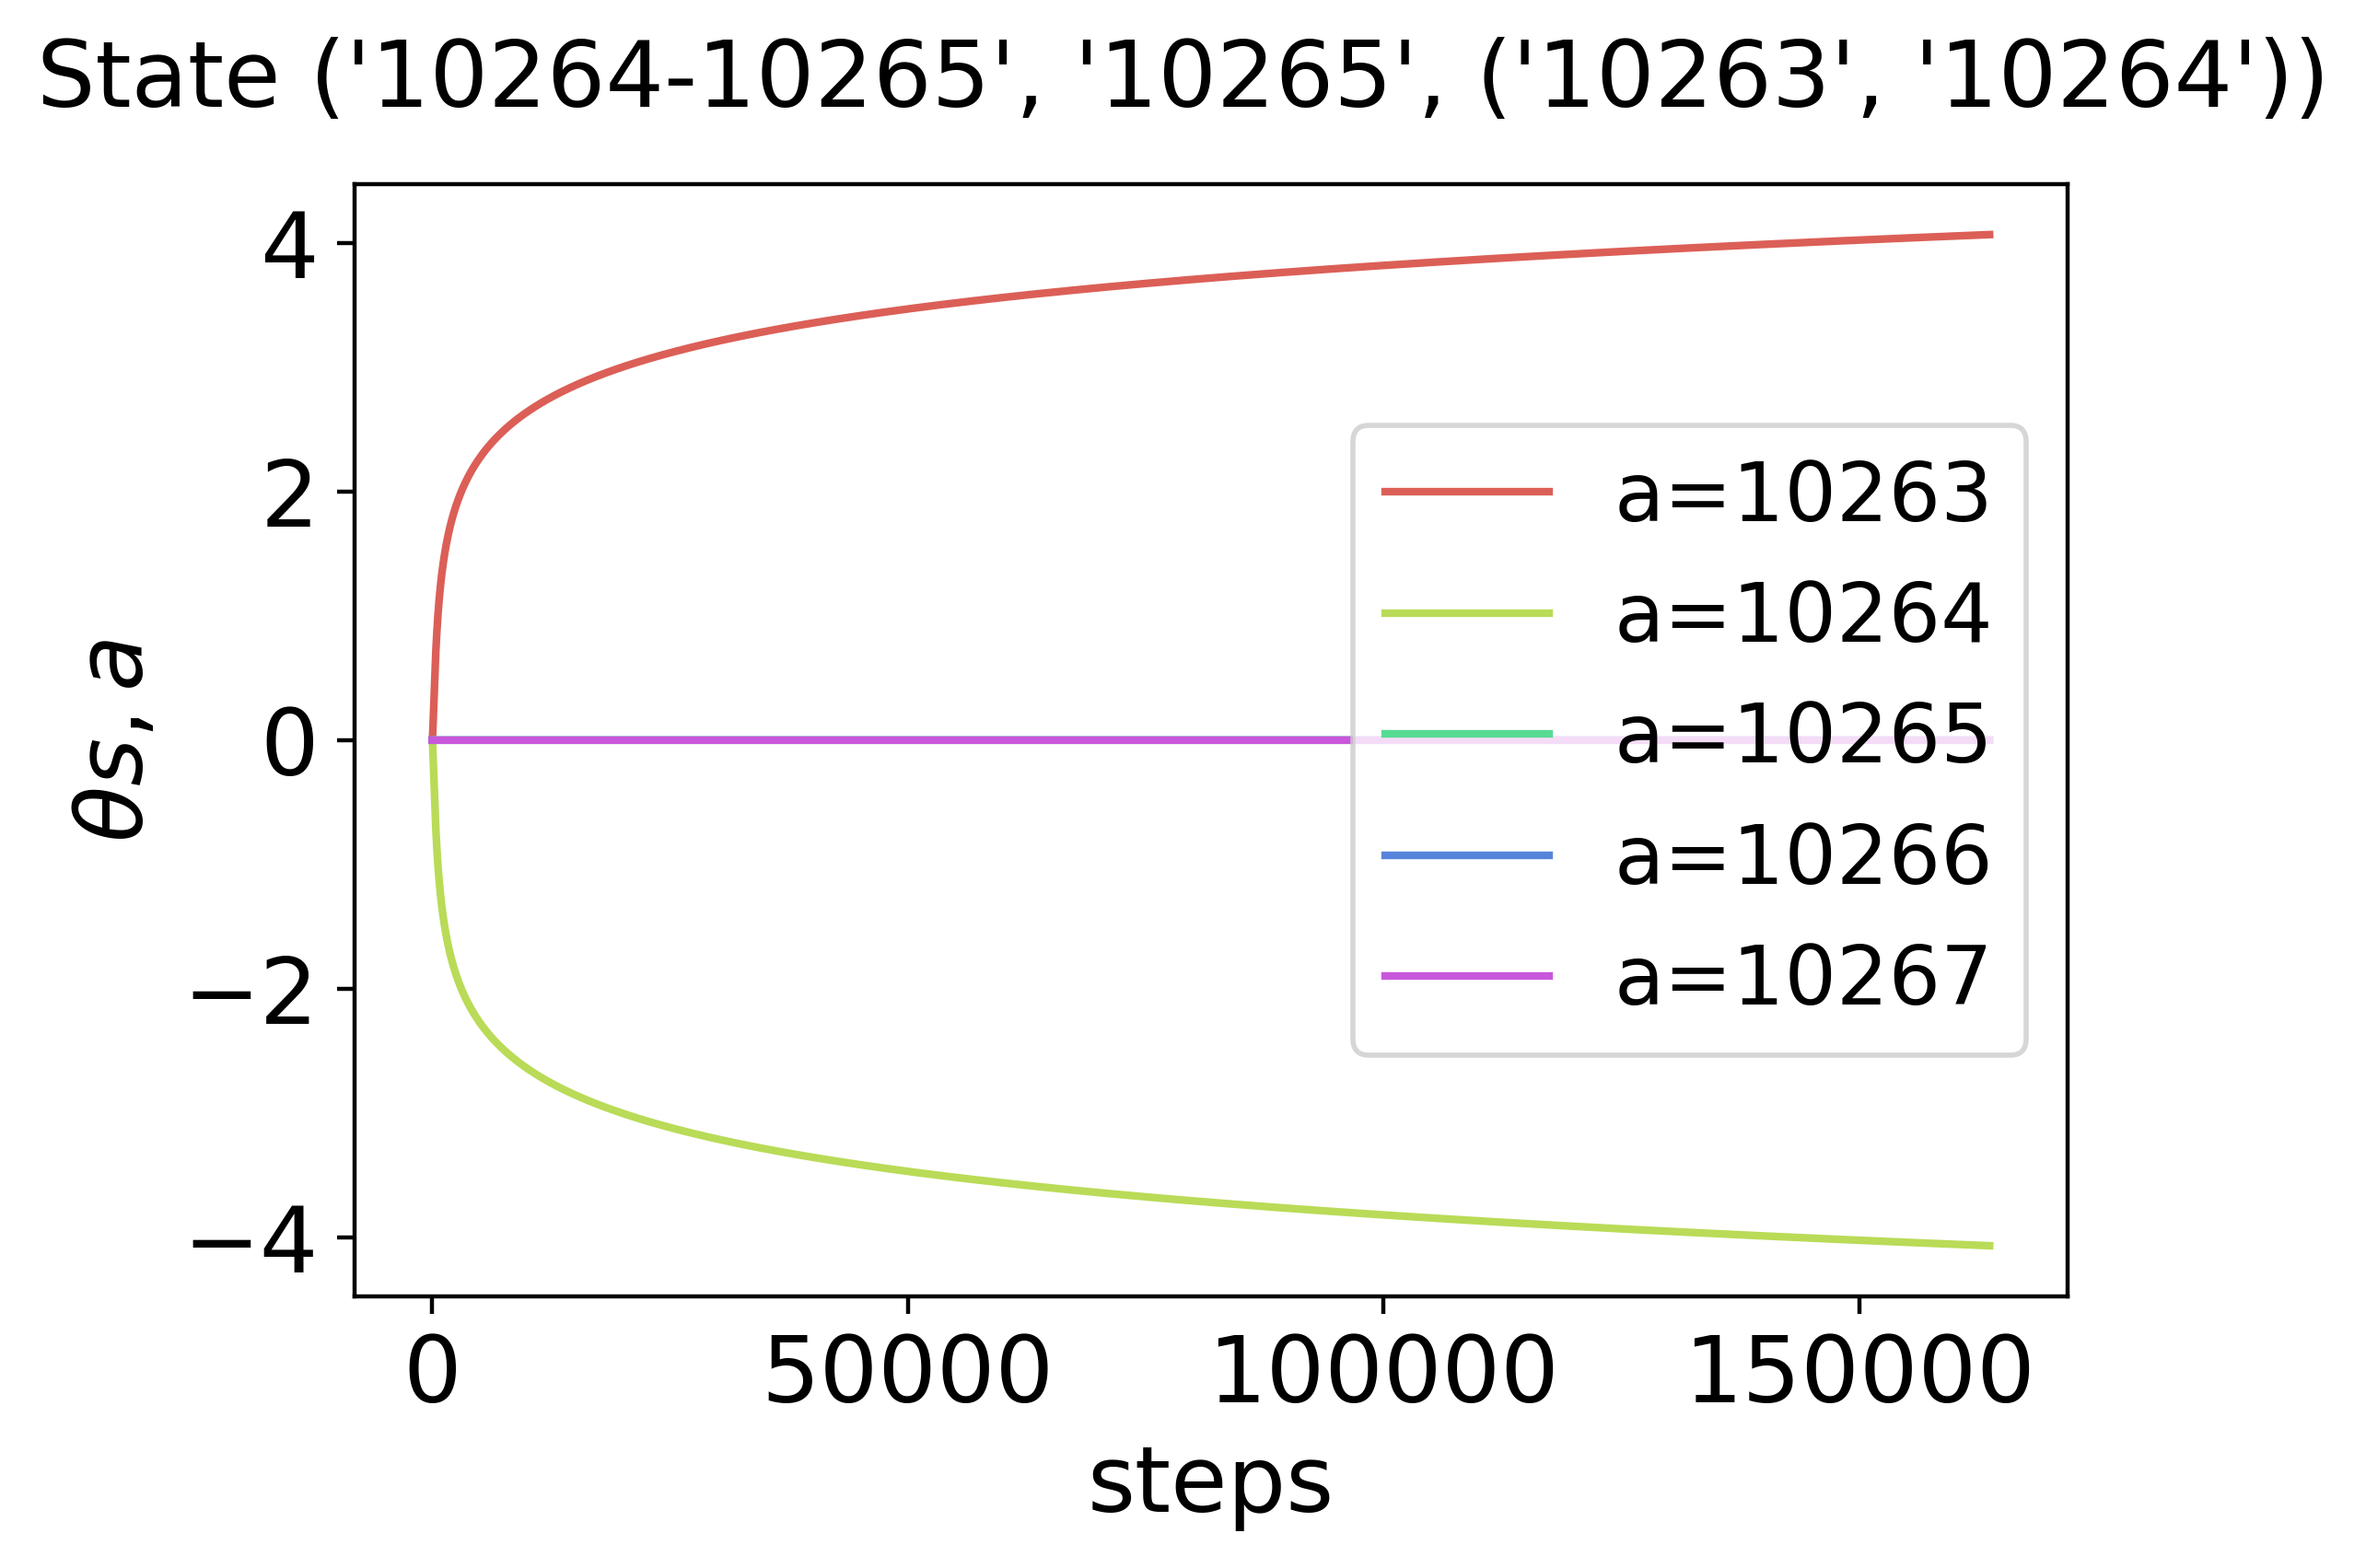
\includegraphics[height=0.27\textwidth,valign=b]{chapters/figures/theta_PG_state_1.png} \\
        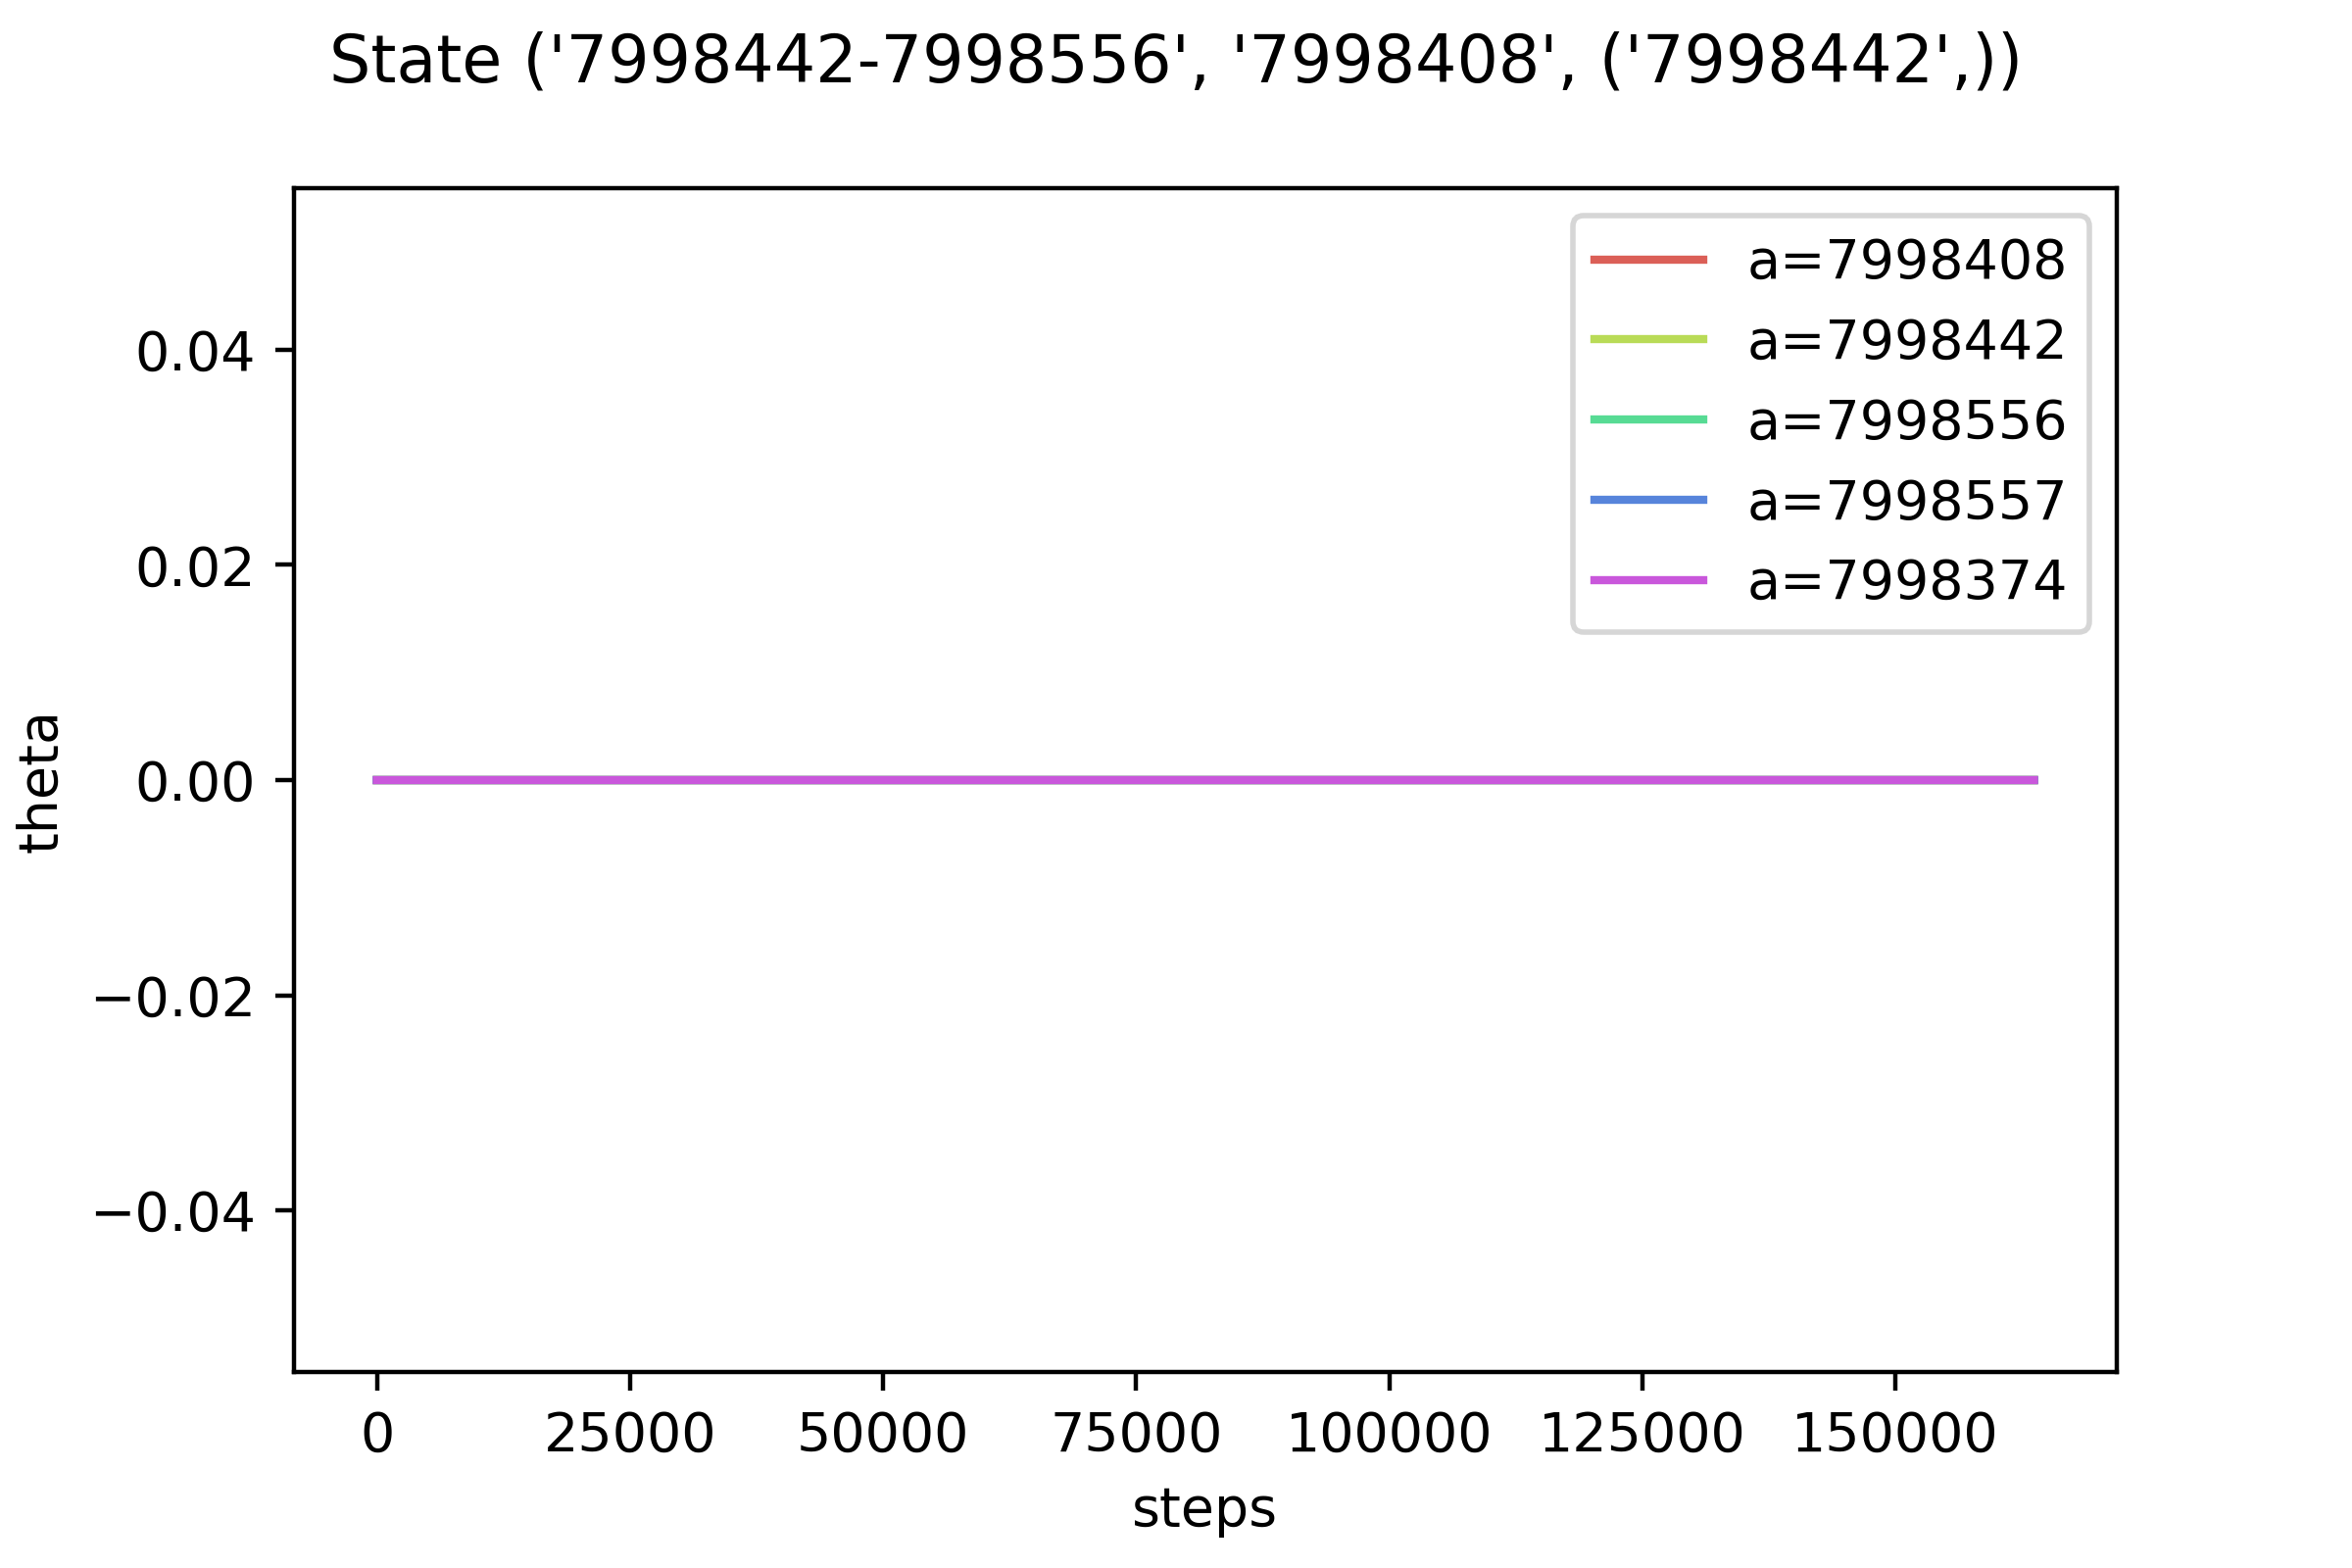
\includegraphics[height=0.27\textwidth,valign=b]{chapters/figures/theta_PG_state_2.png} &
        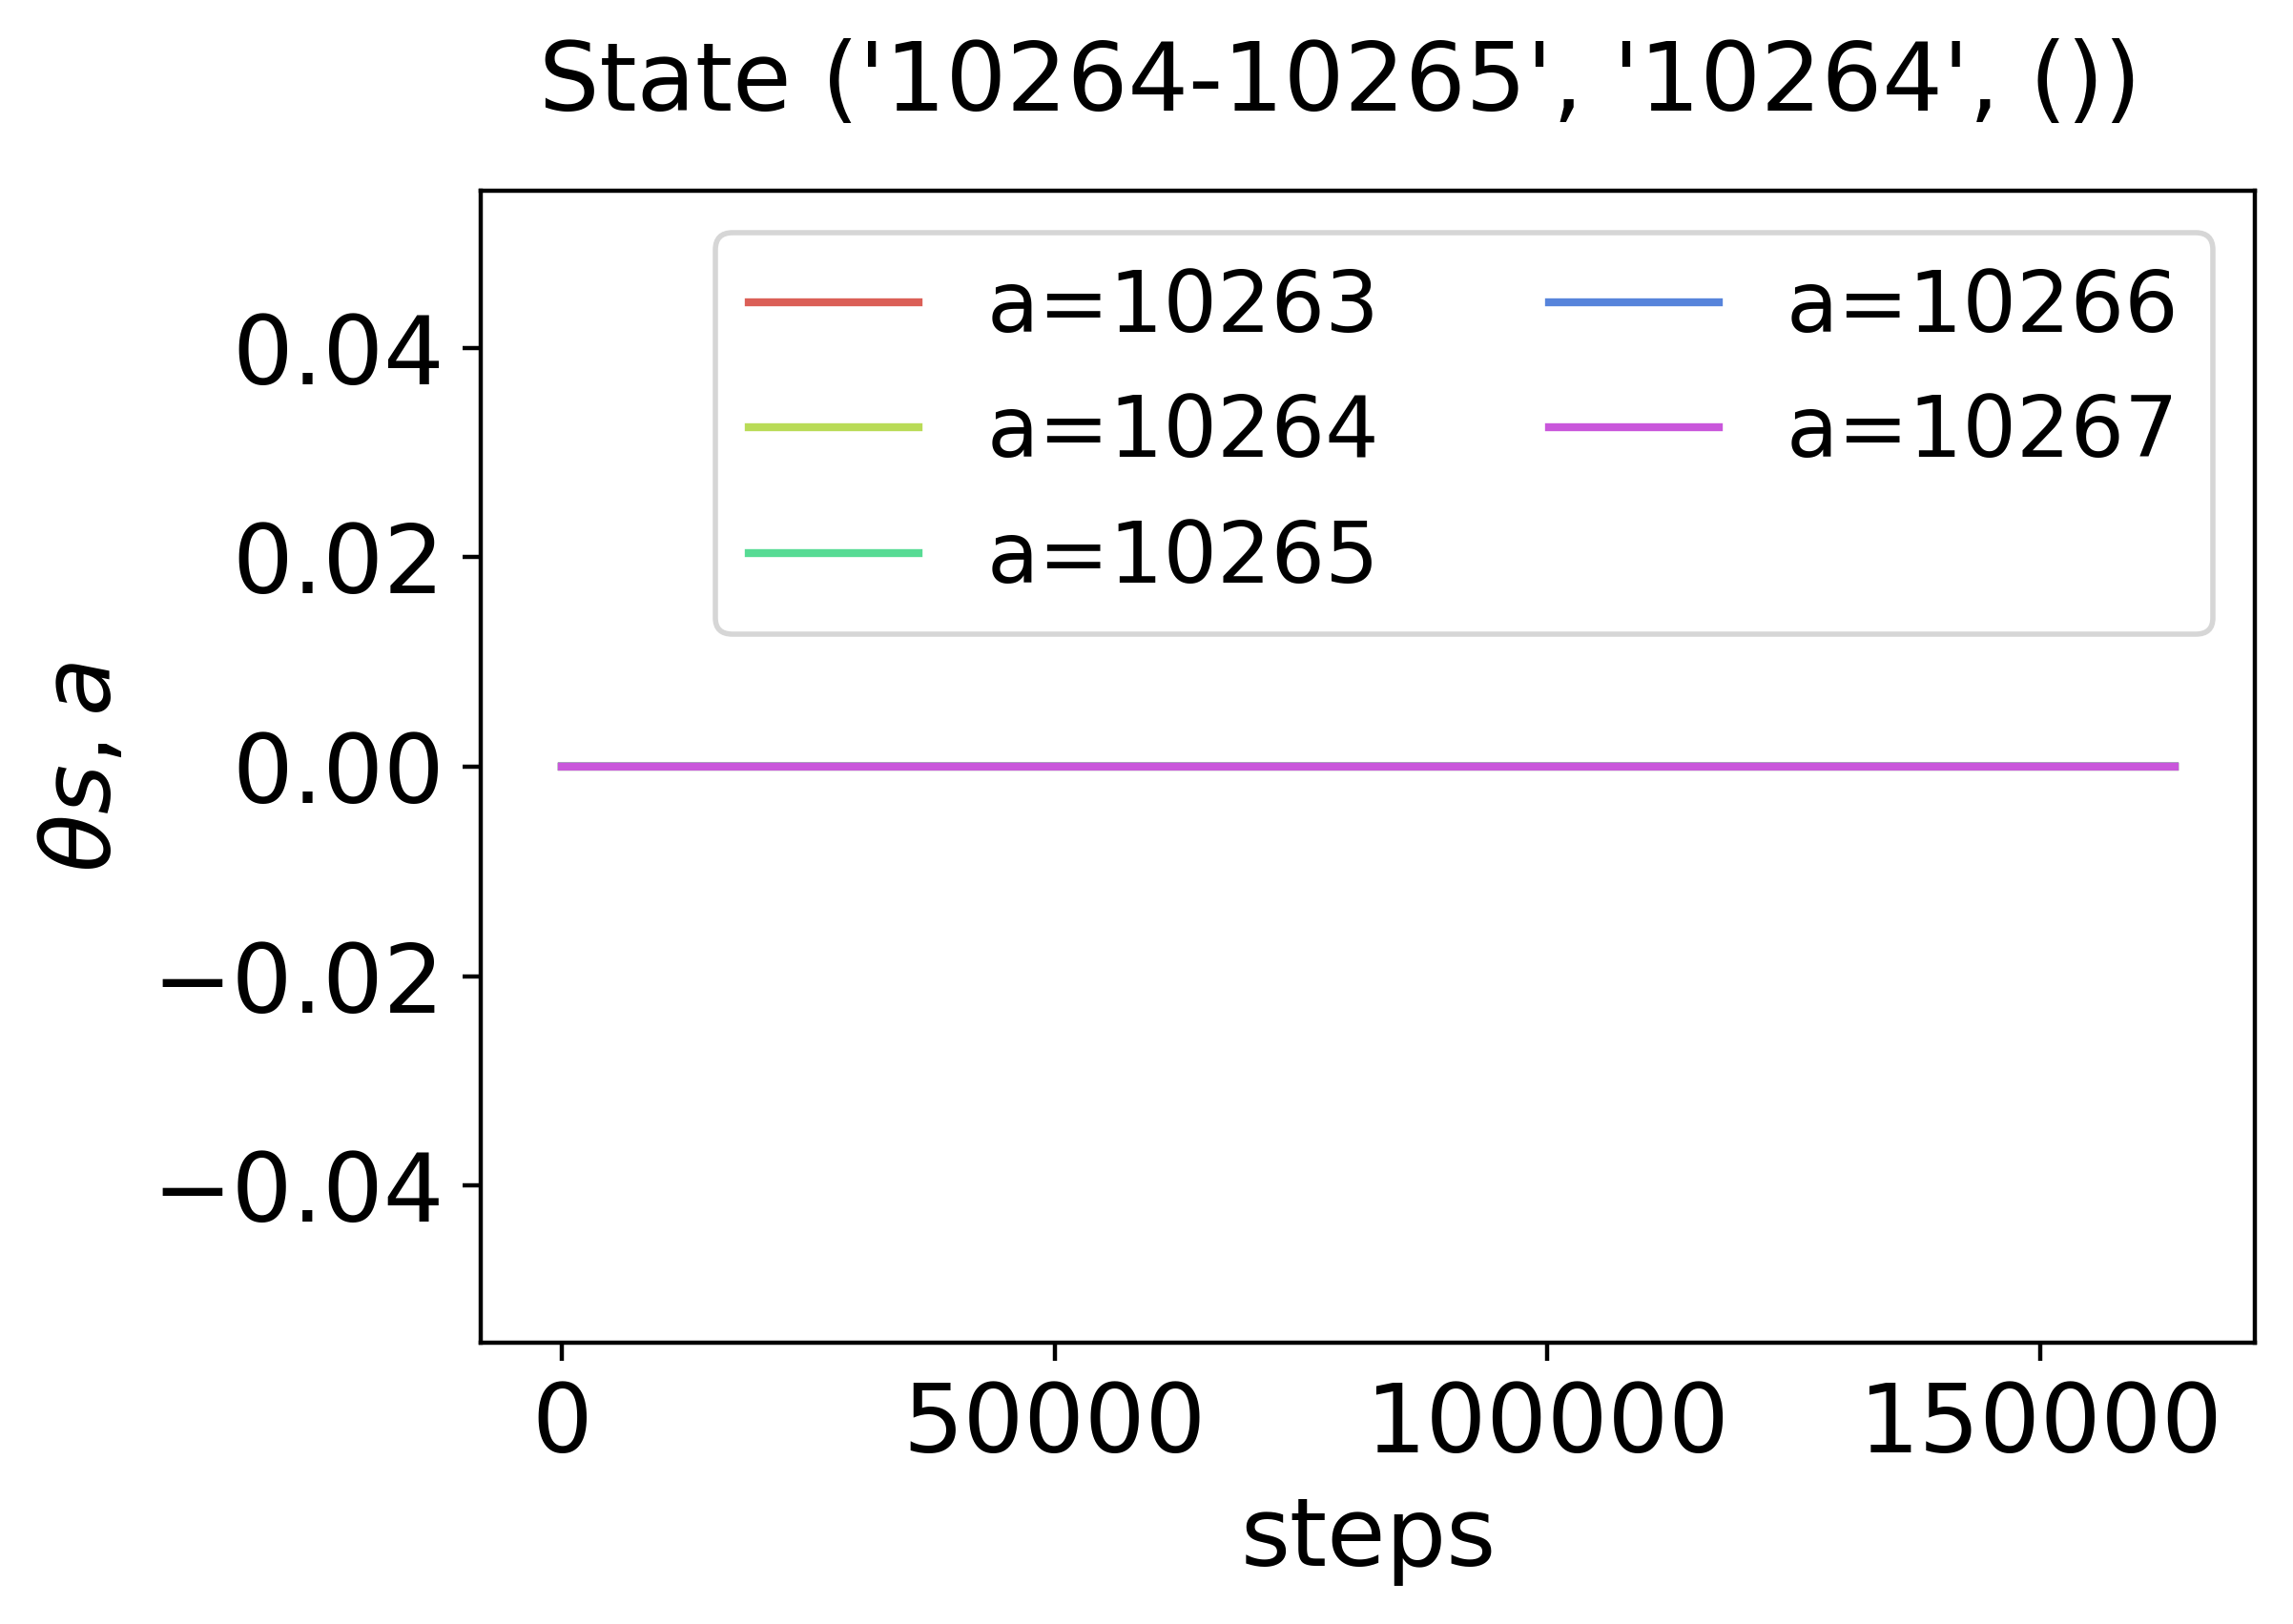
\includegraphics[height=0.27\textwidth,valign=b]{chapters/figures/theta_PG_state_3.png}
    \end{tabular}
    \caption{Trajectories of the parameters $\boldsymbol \theta$ in the parameters space for \acrshort{pg}, for a specific episode with $5$ initially disconnected substation.}
    \label{fig:sequence-theta-pg}
\end{figure}

\begin{figure}[!htp]
    \centering
    \begin{tabular}{cc}
        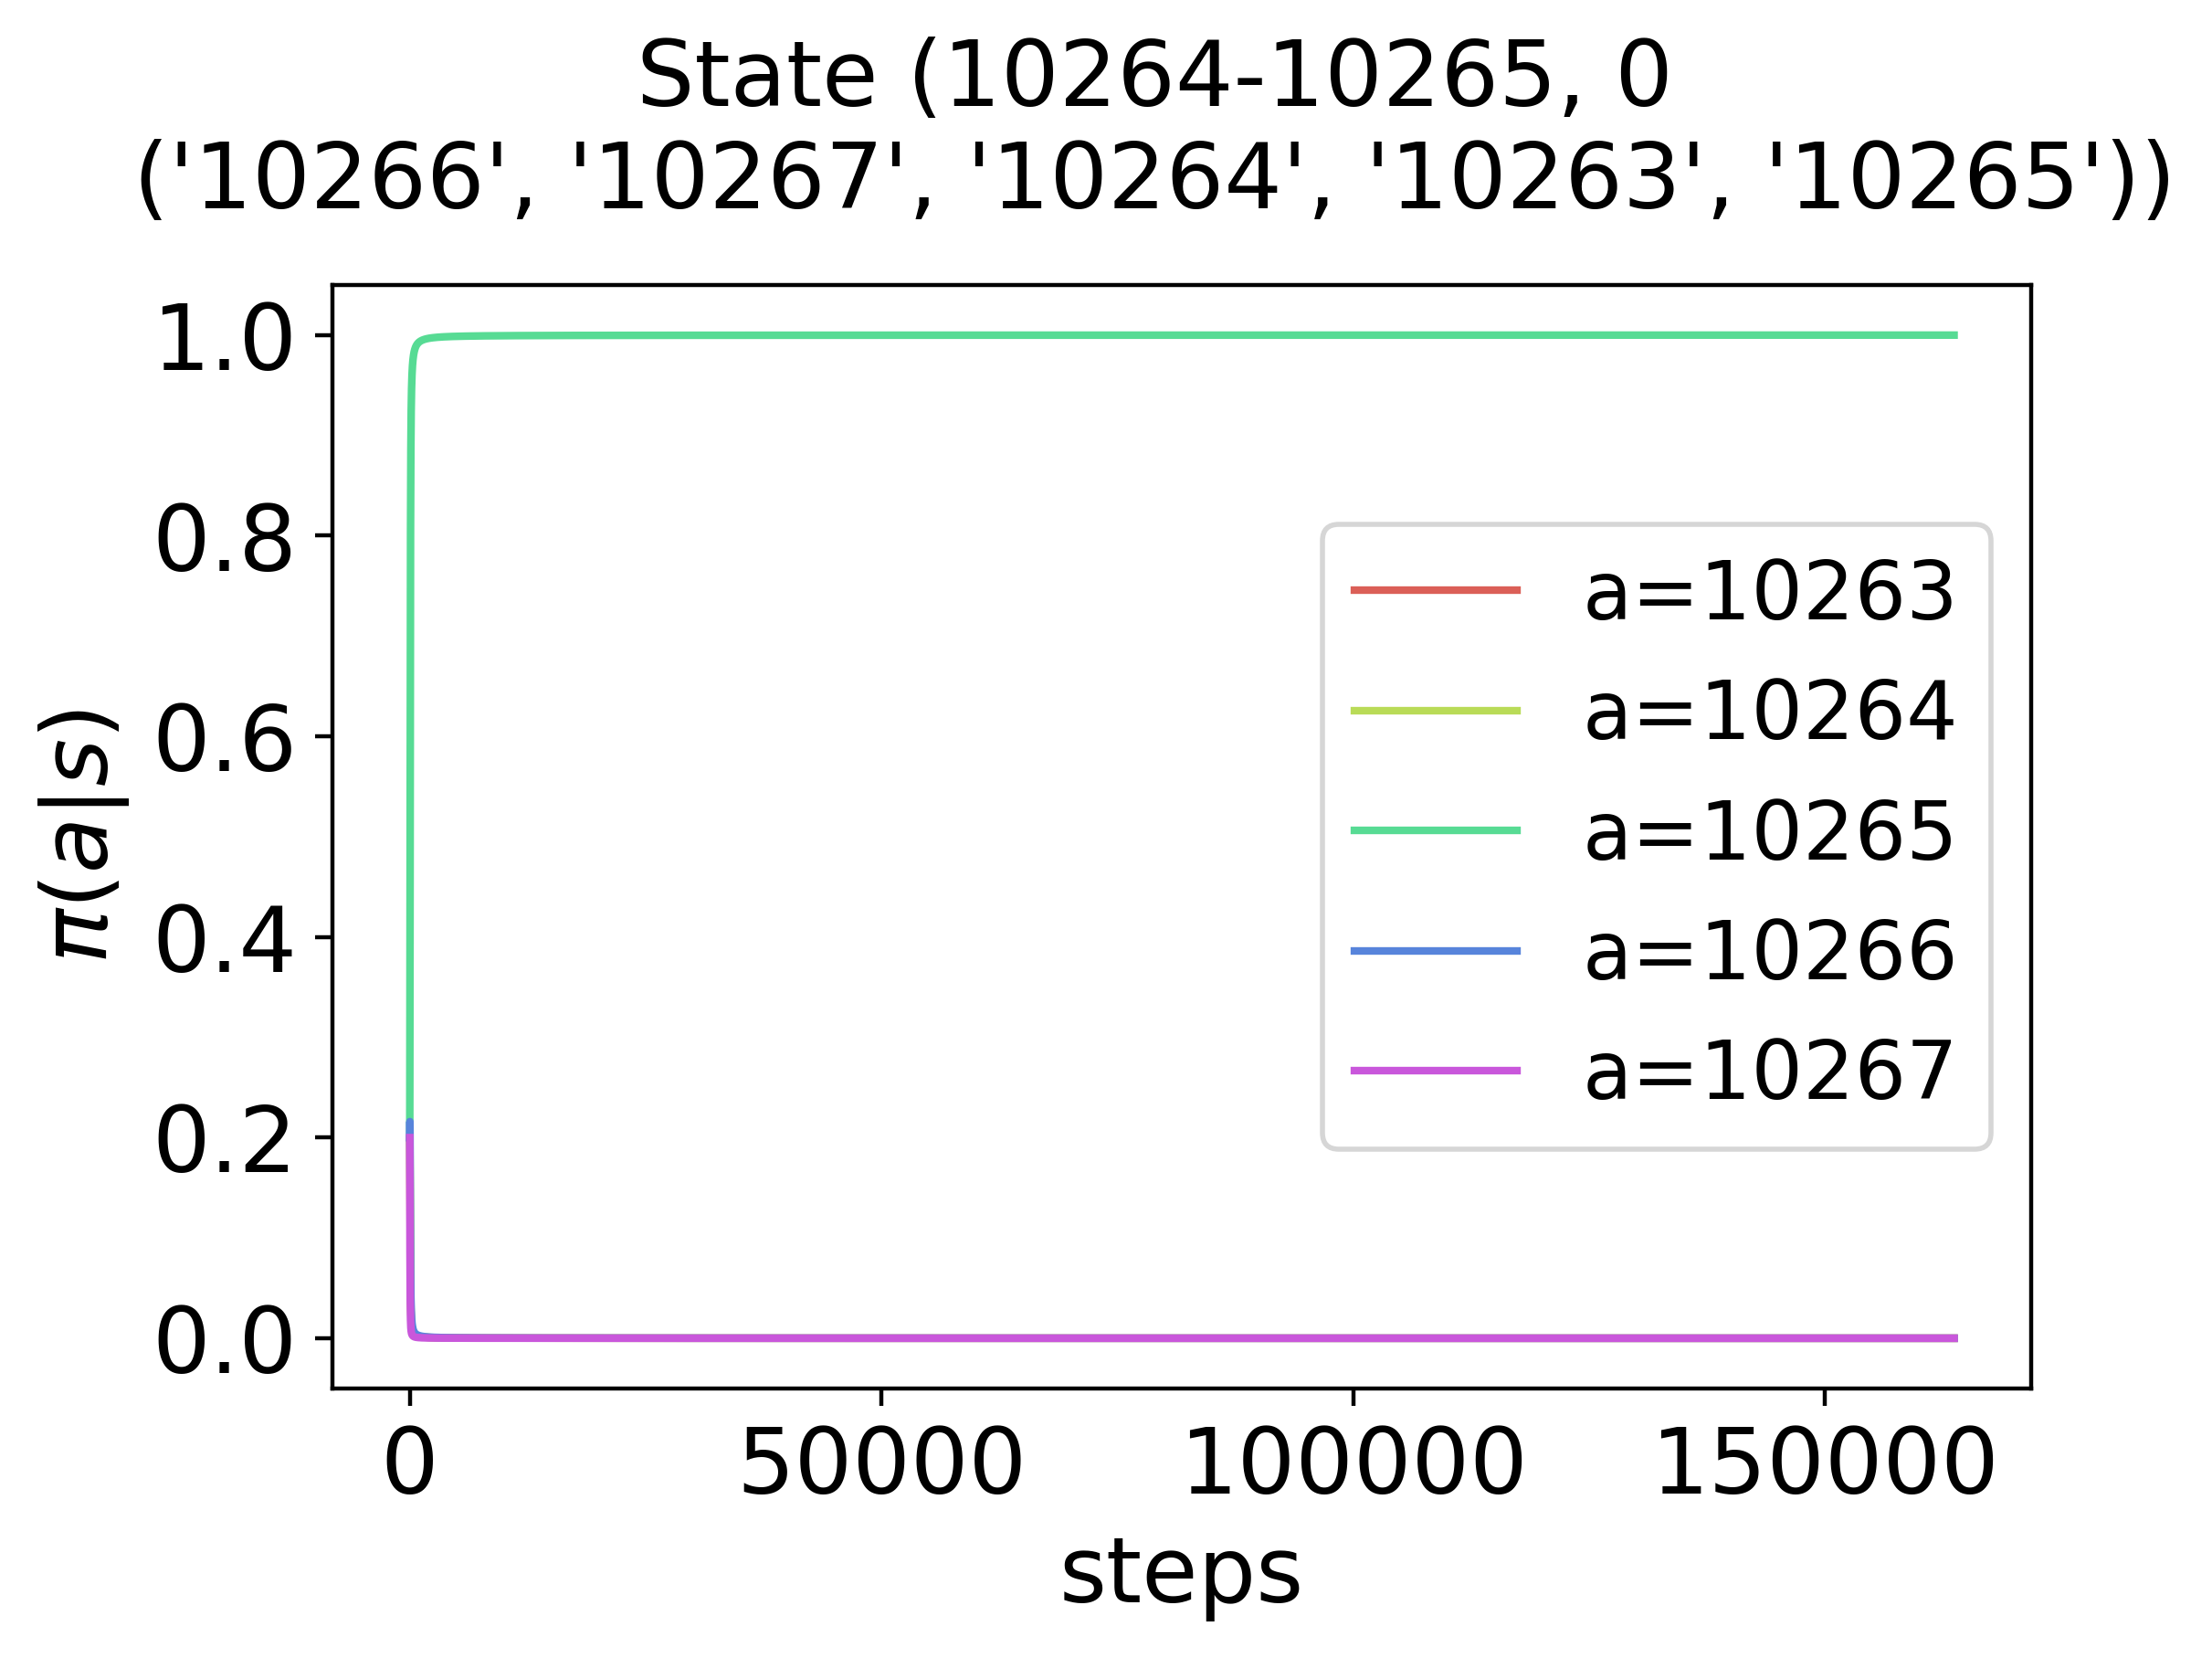
\includegraphics[height=0.27\textwidth,valign=b]{chapters/figures/policy_PG_state_0.png} &
        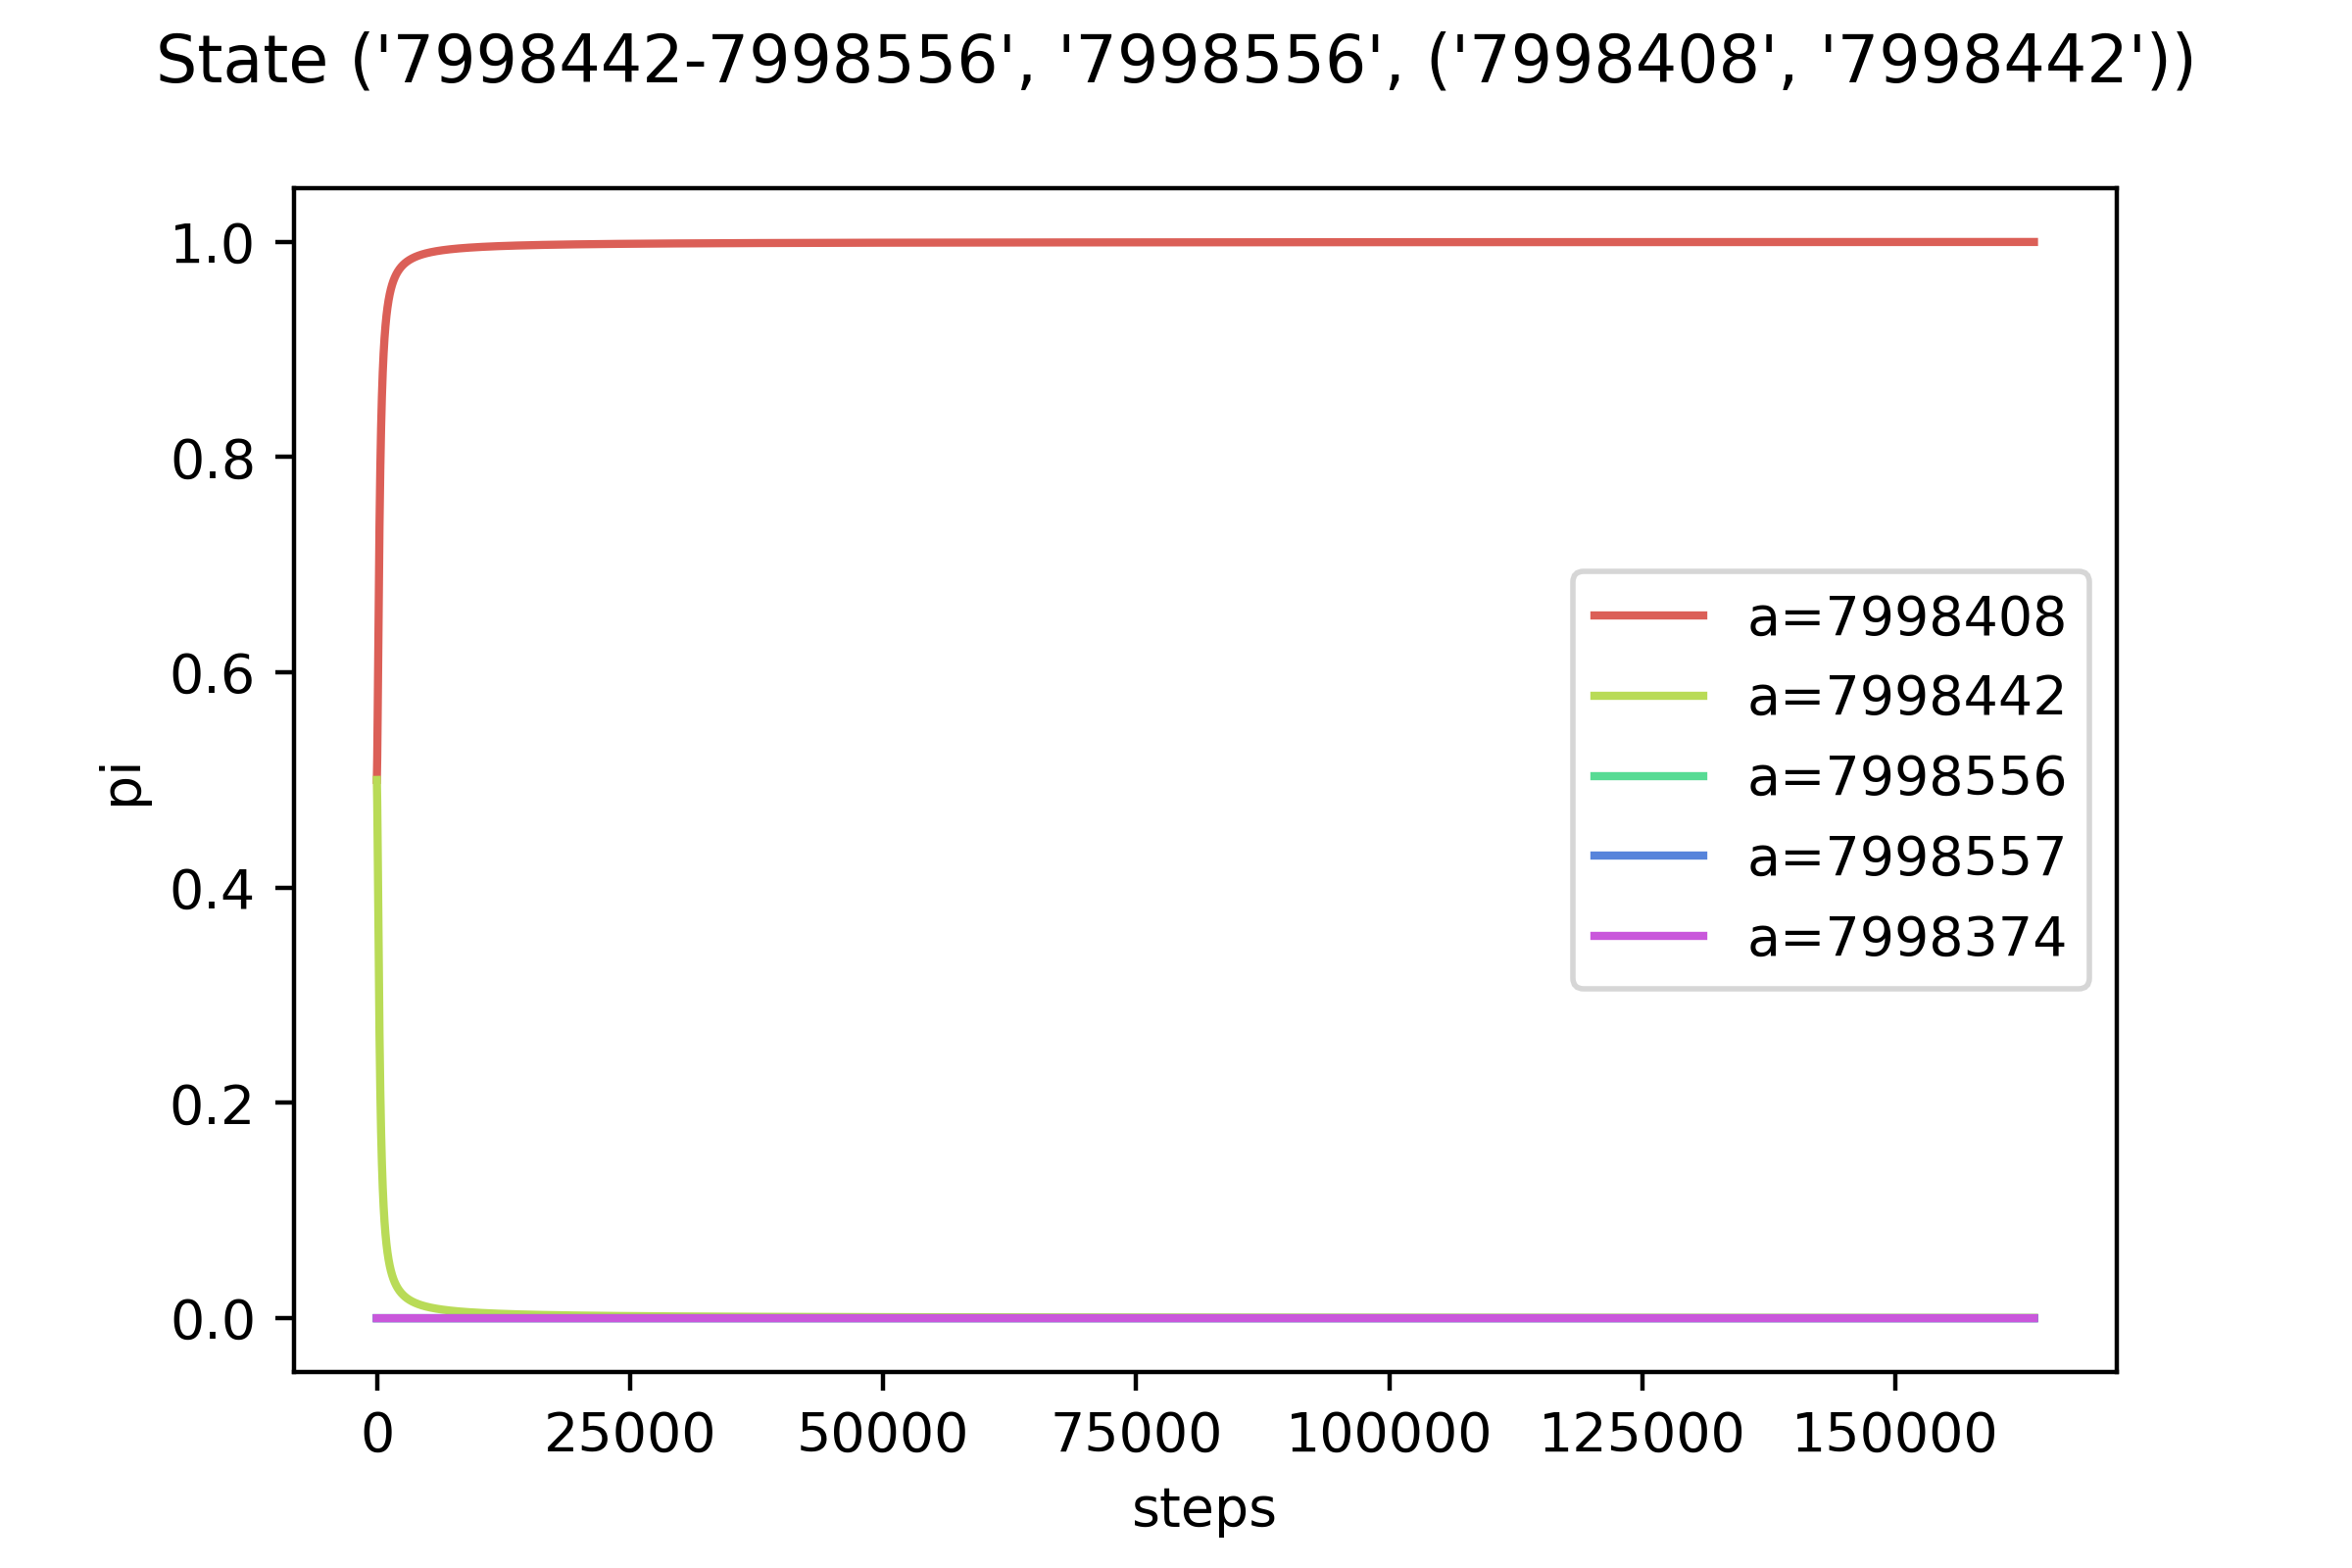
\includegraphics[height=0.27\textwidth,valign=b]{chapters/figures/policy_PG_state_1.png} \\
        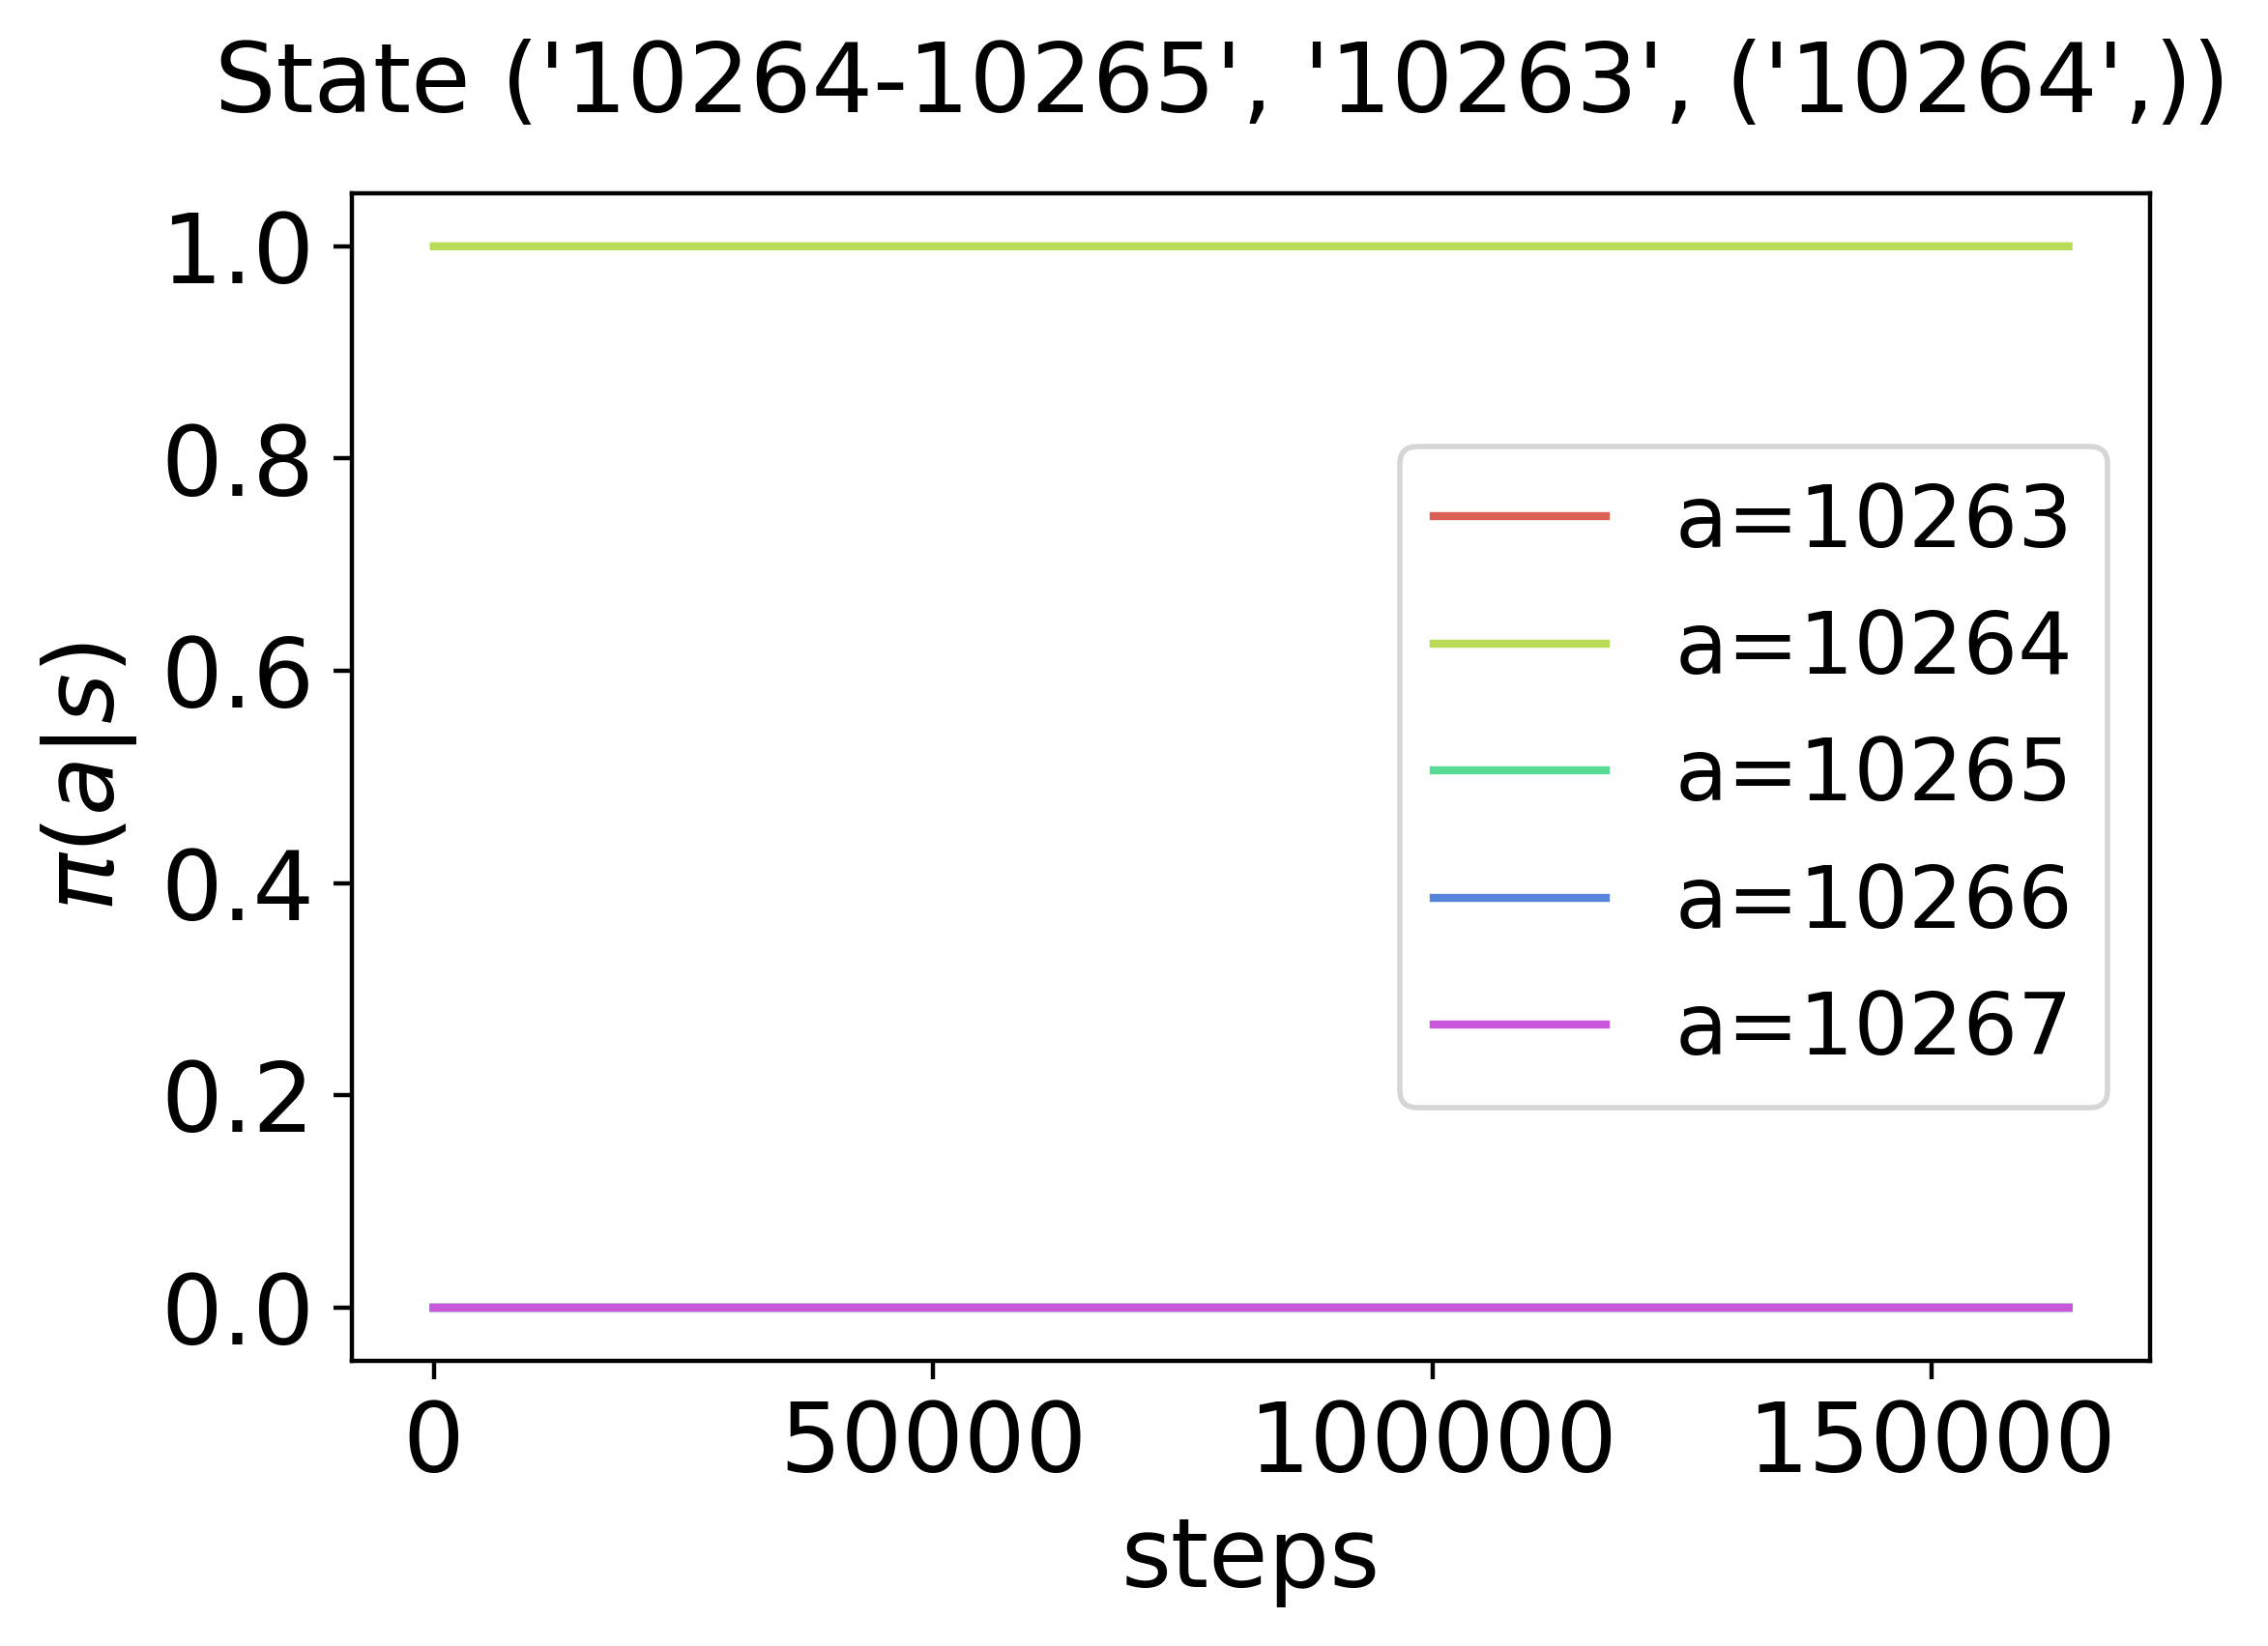
\includegraphics[height=0.27\textwidth,valign=b]{chapters/figures/policy_PG_state_2.png} &
        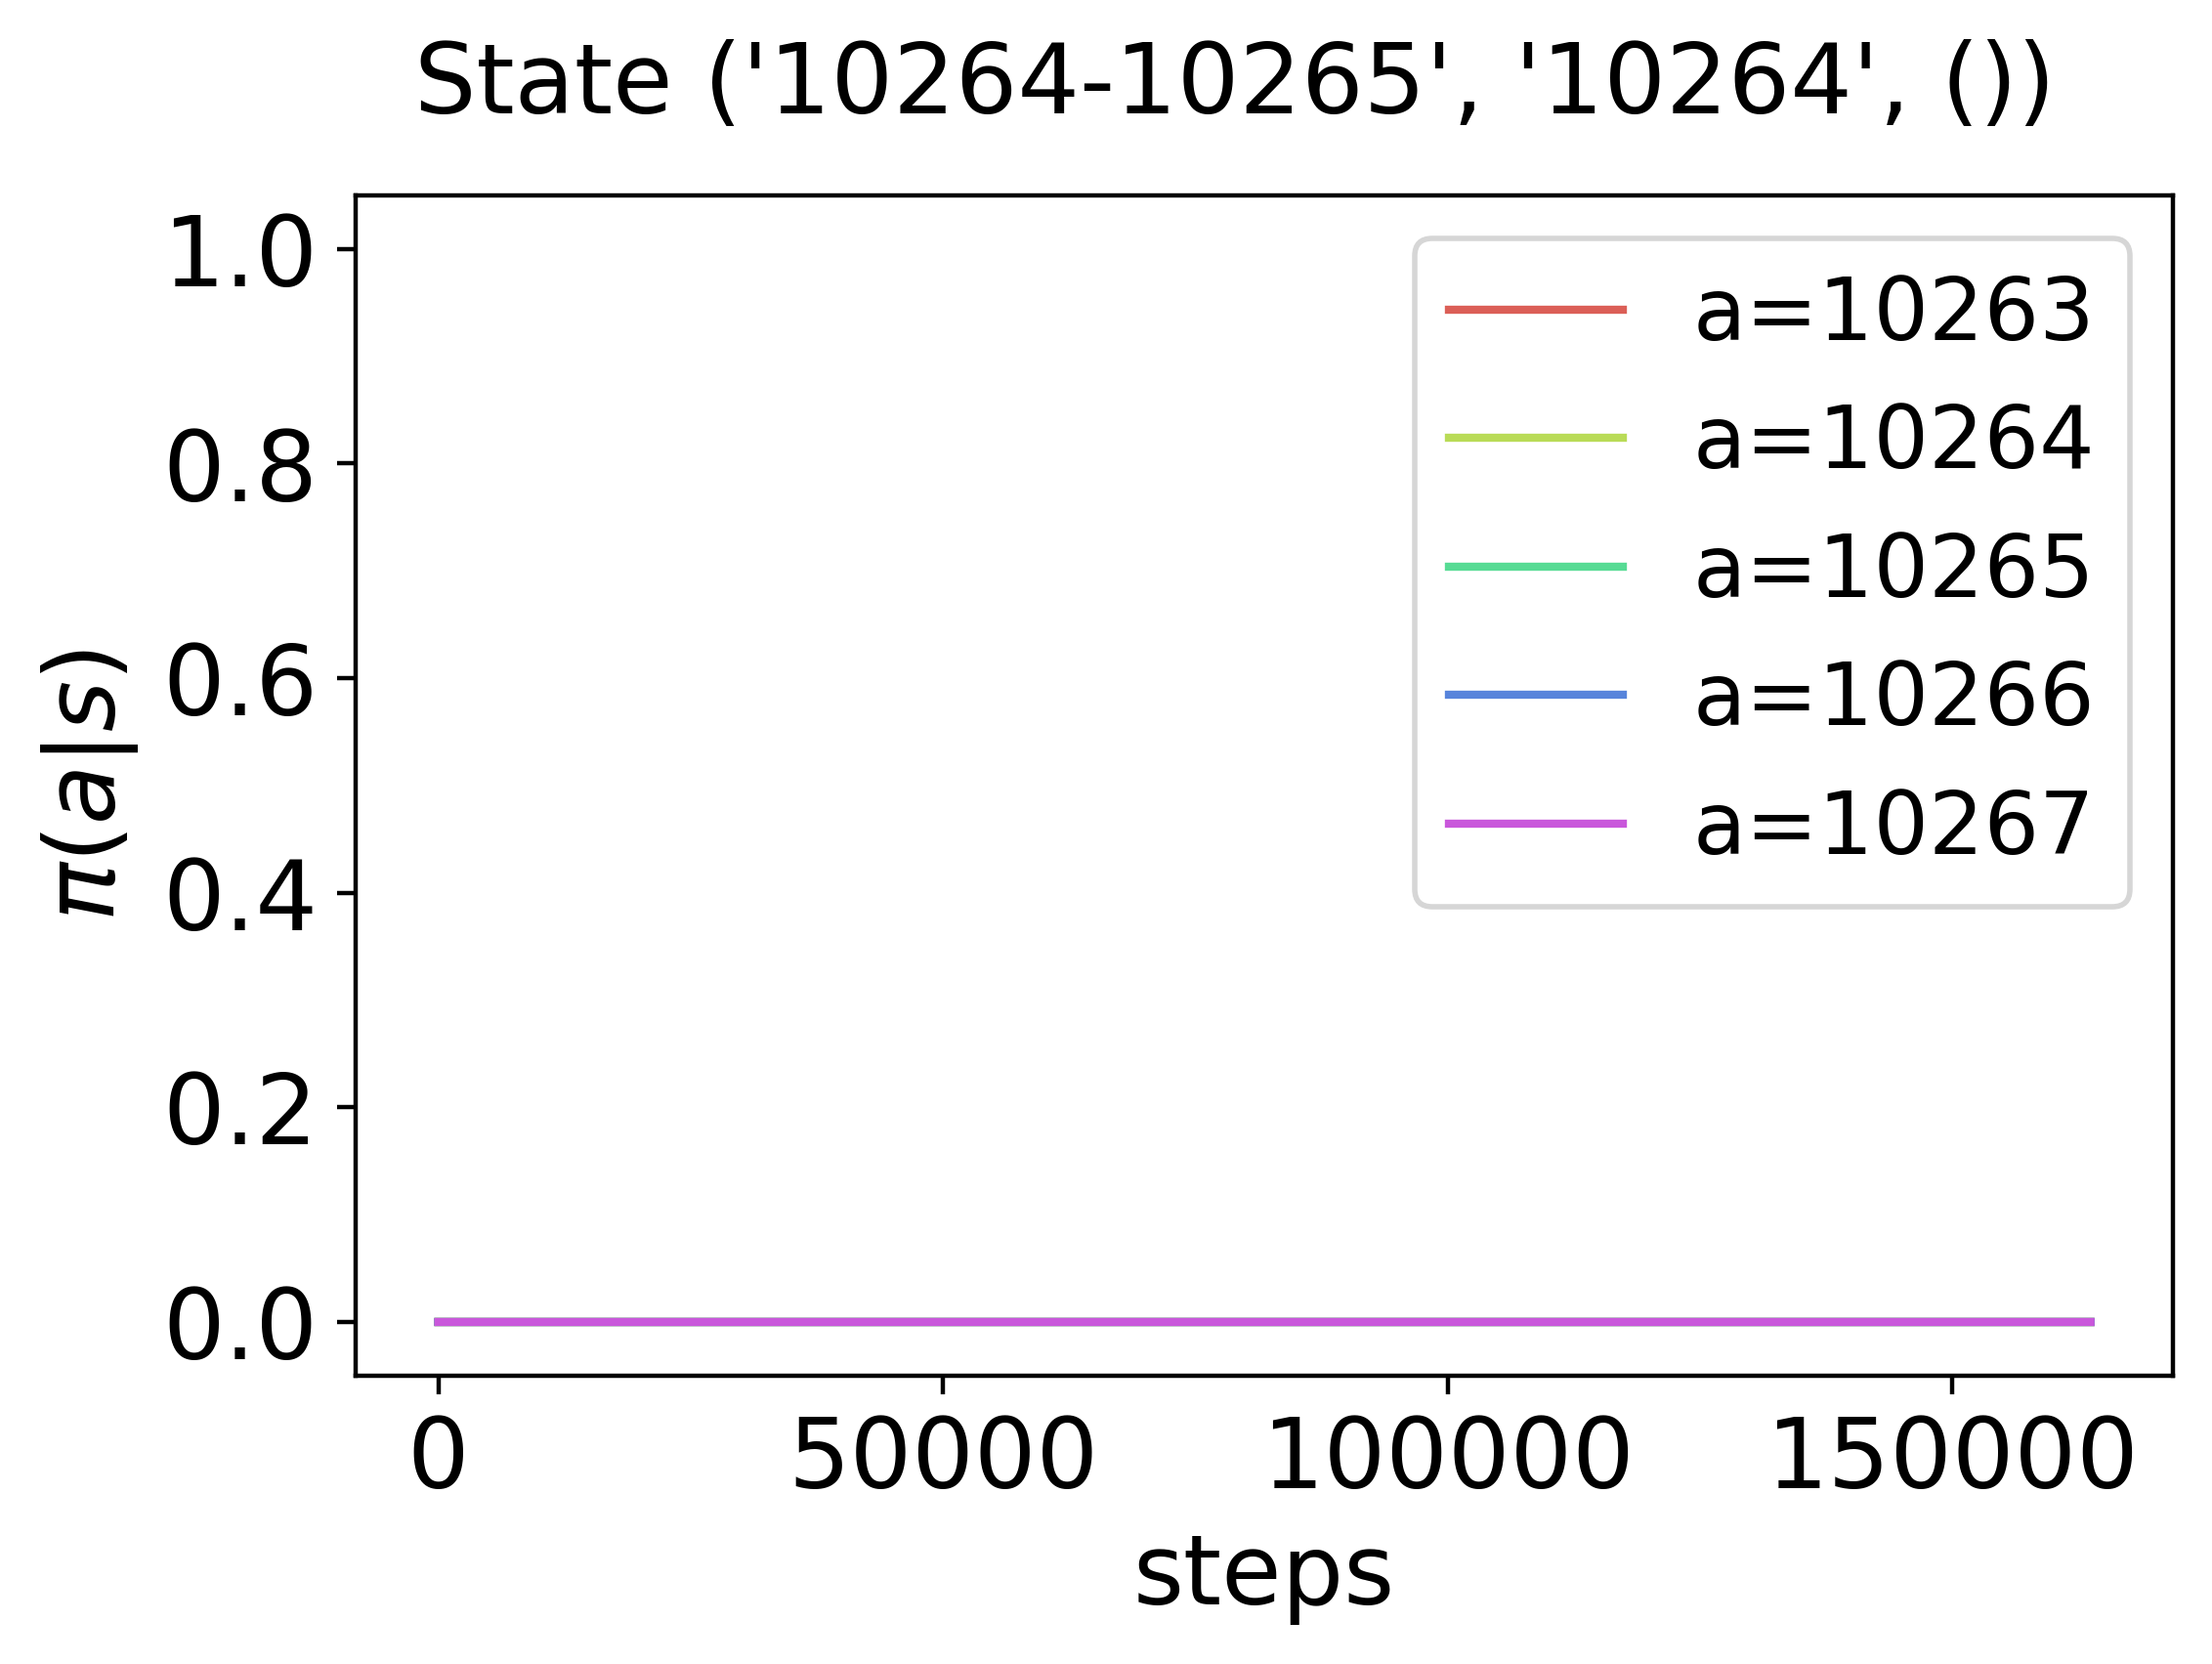
\includegraphics[height=0.27\textwidth,valign=b]{chapters/figures/policy_PG_state_3.png}
    \end{tabular}
    \caption{Trajectories of the policies $\pi_{\boldsymbol \theta}$ in the policy space for \acrshort{pg}, for a specific episode with $5$ initially disconnected substation.}
    \label{fig:sequence-policies-pg}
\end{figure}

\begin{figure}[!htp]
    \centering
    \begin{tabular}{cc}
        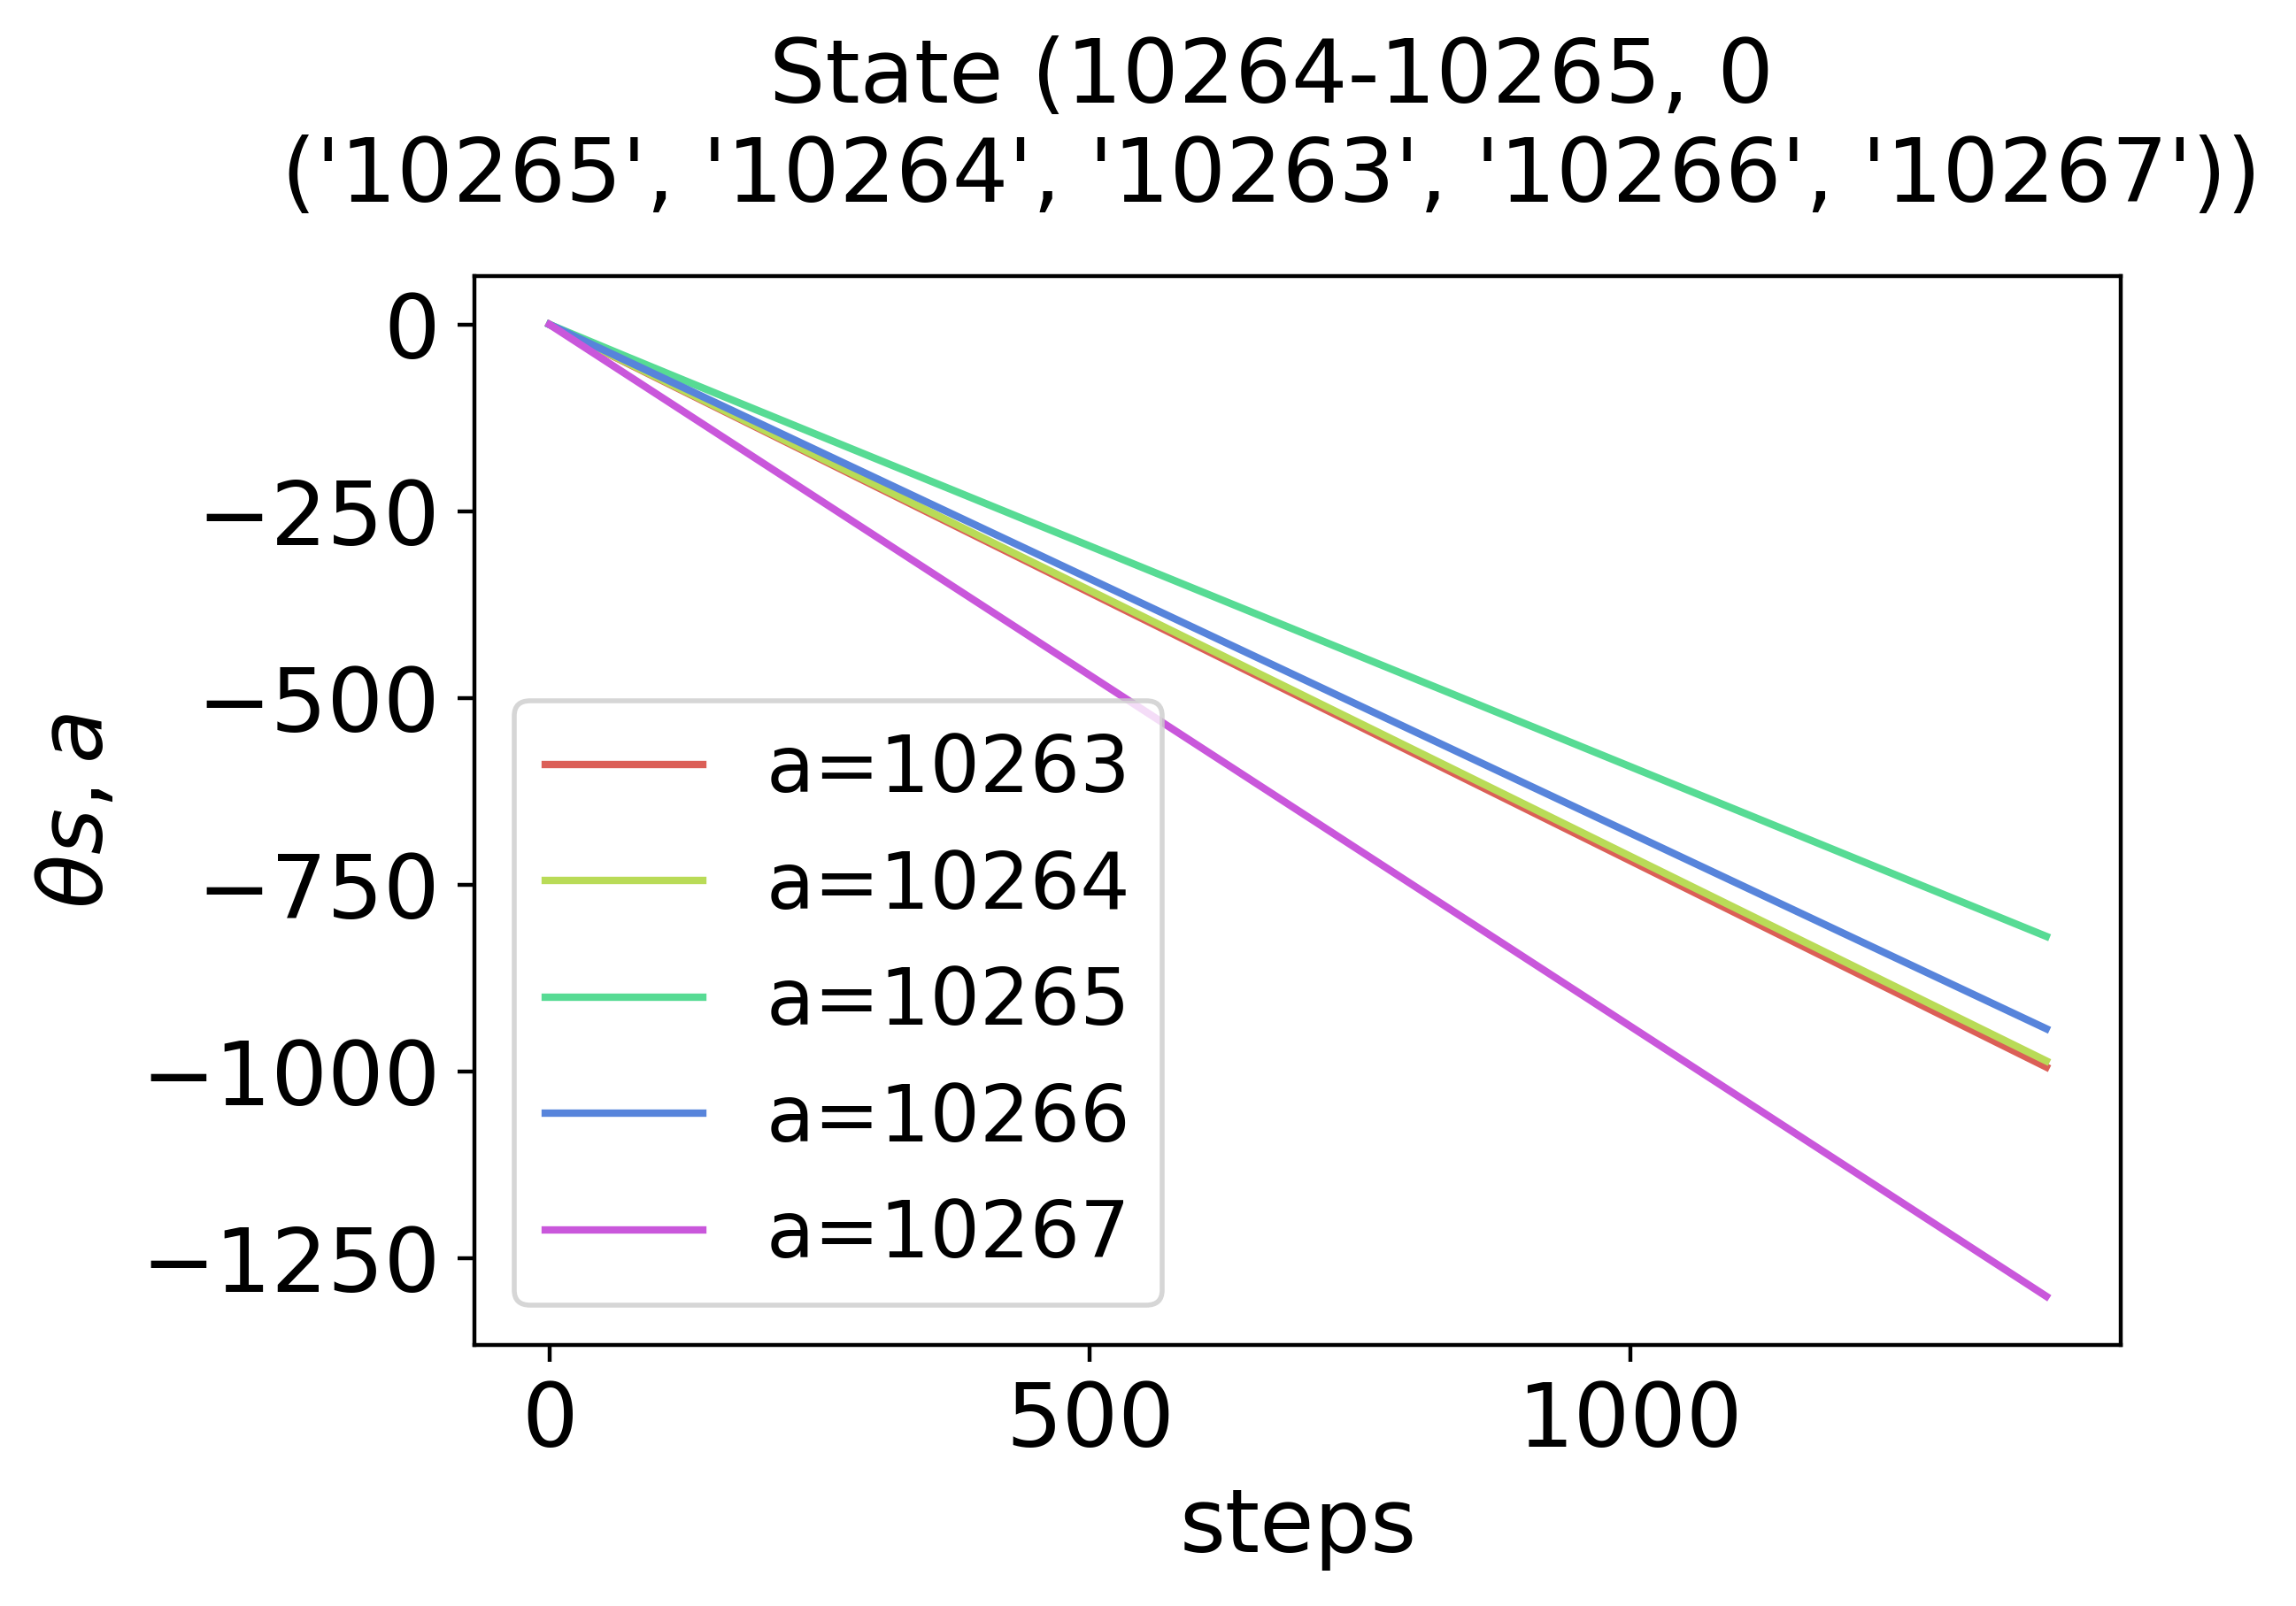
\includegraphics[height=0.27\textwidth,valign=b]{chapters/figures/theta_NPG_state_0.png} &
        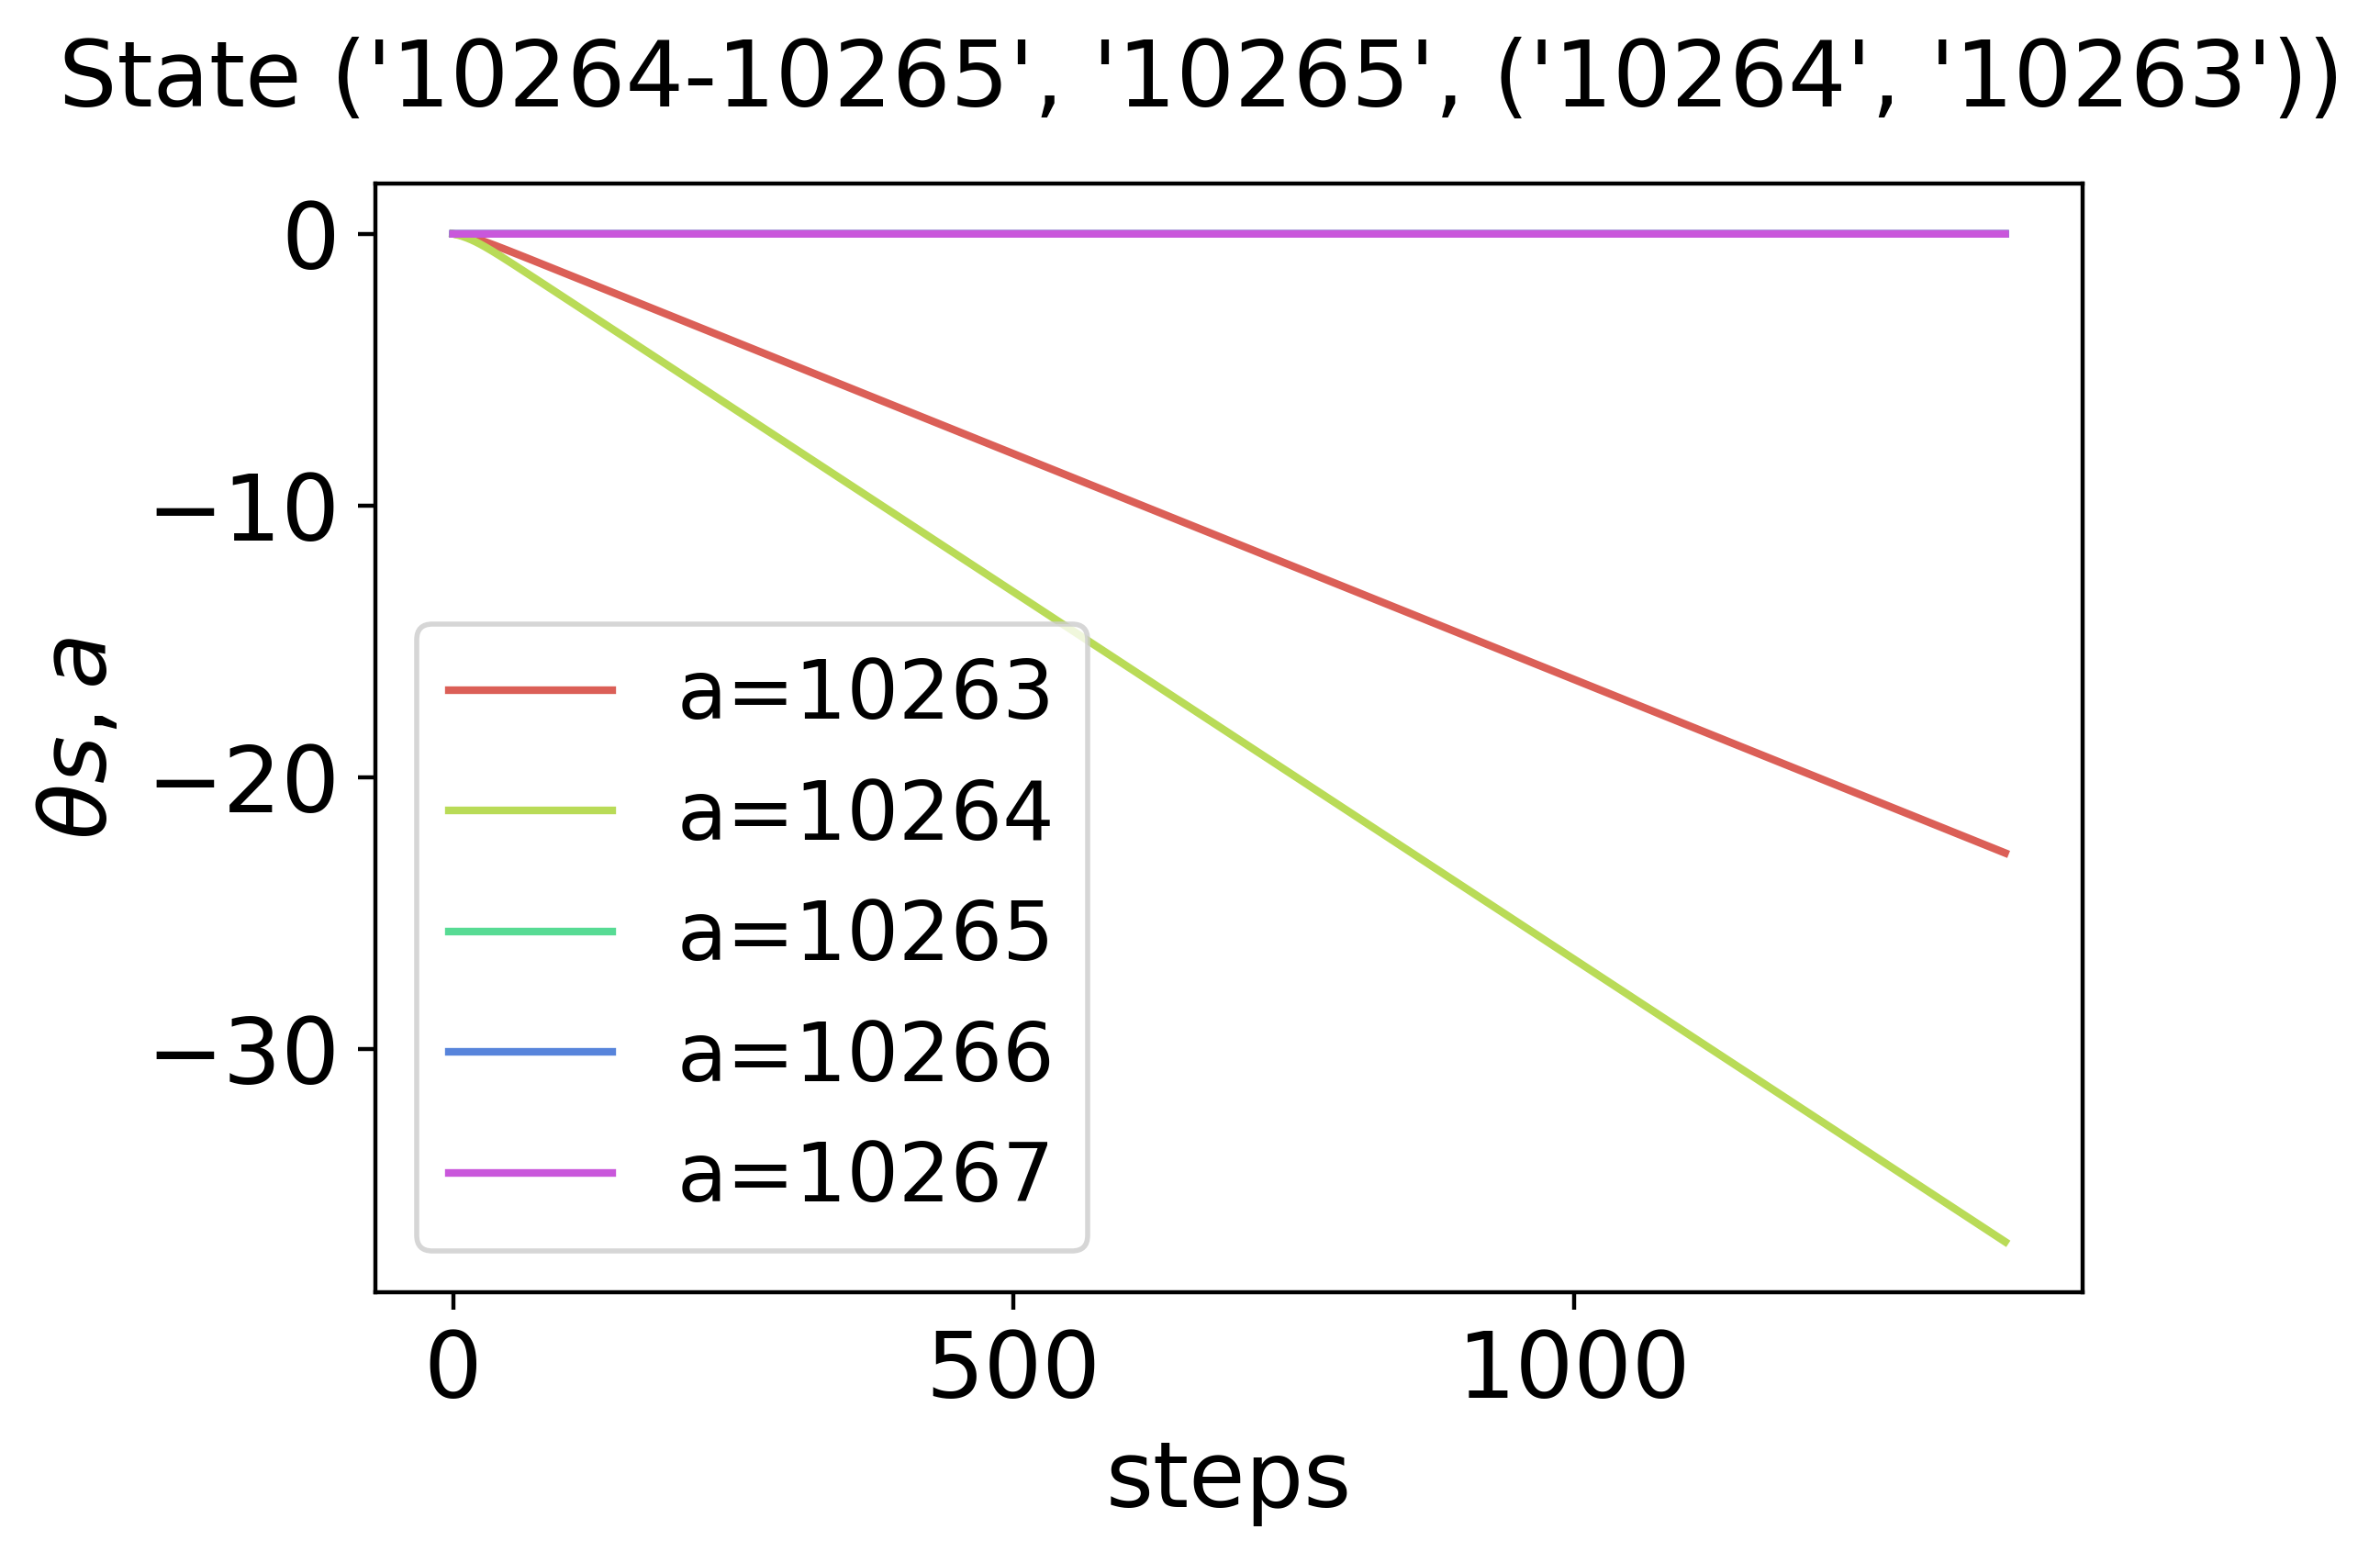
\includegraphics[height=0.27\textwidth,valign=b]{chapters/figures/theta_NPG_state_1.png} \\
        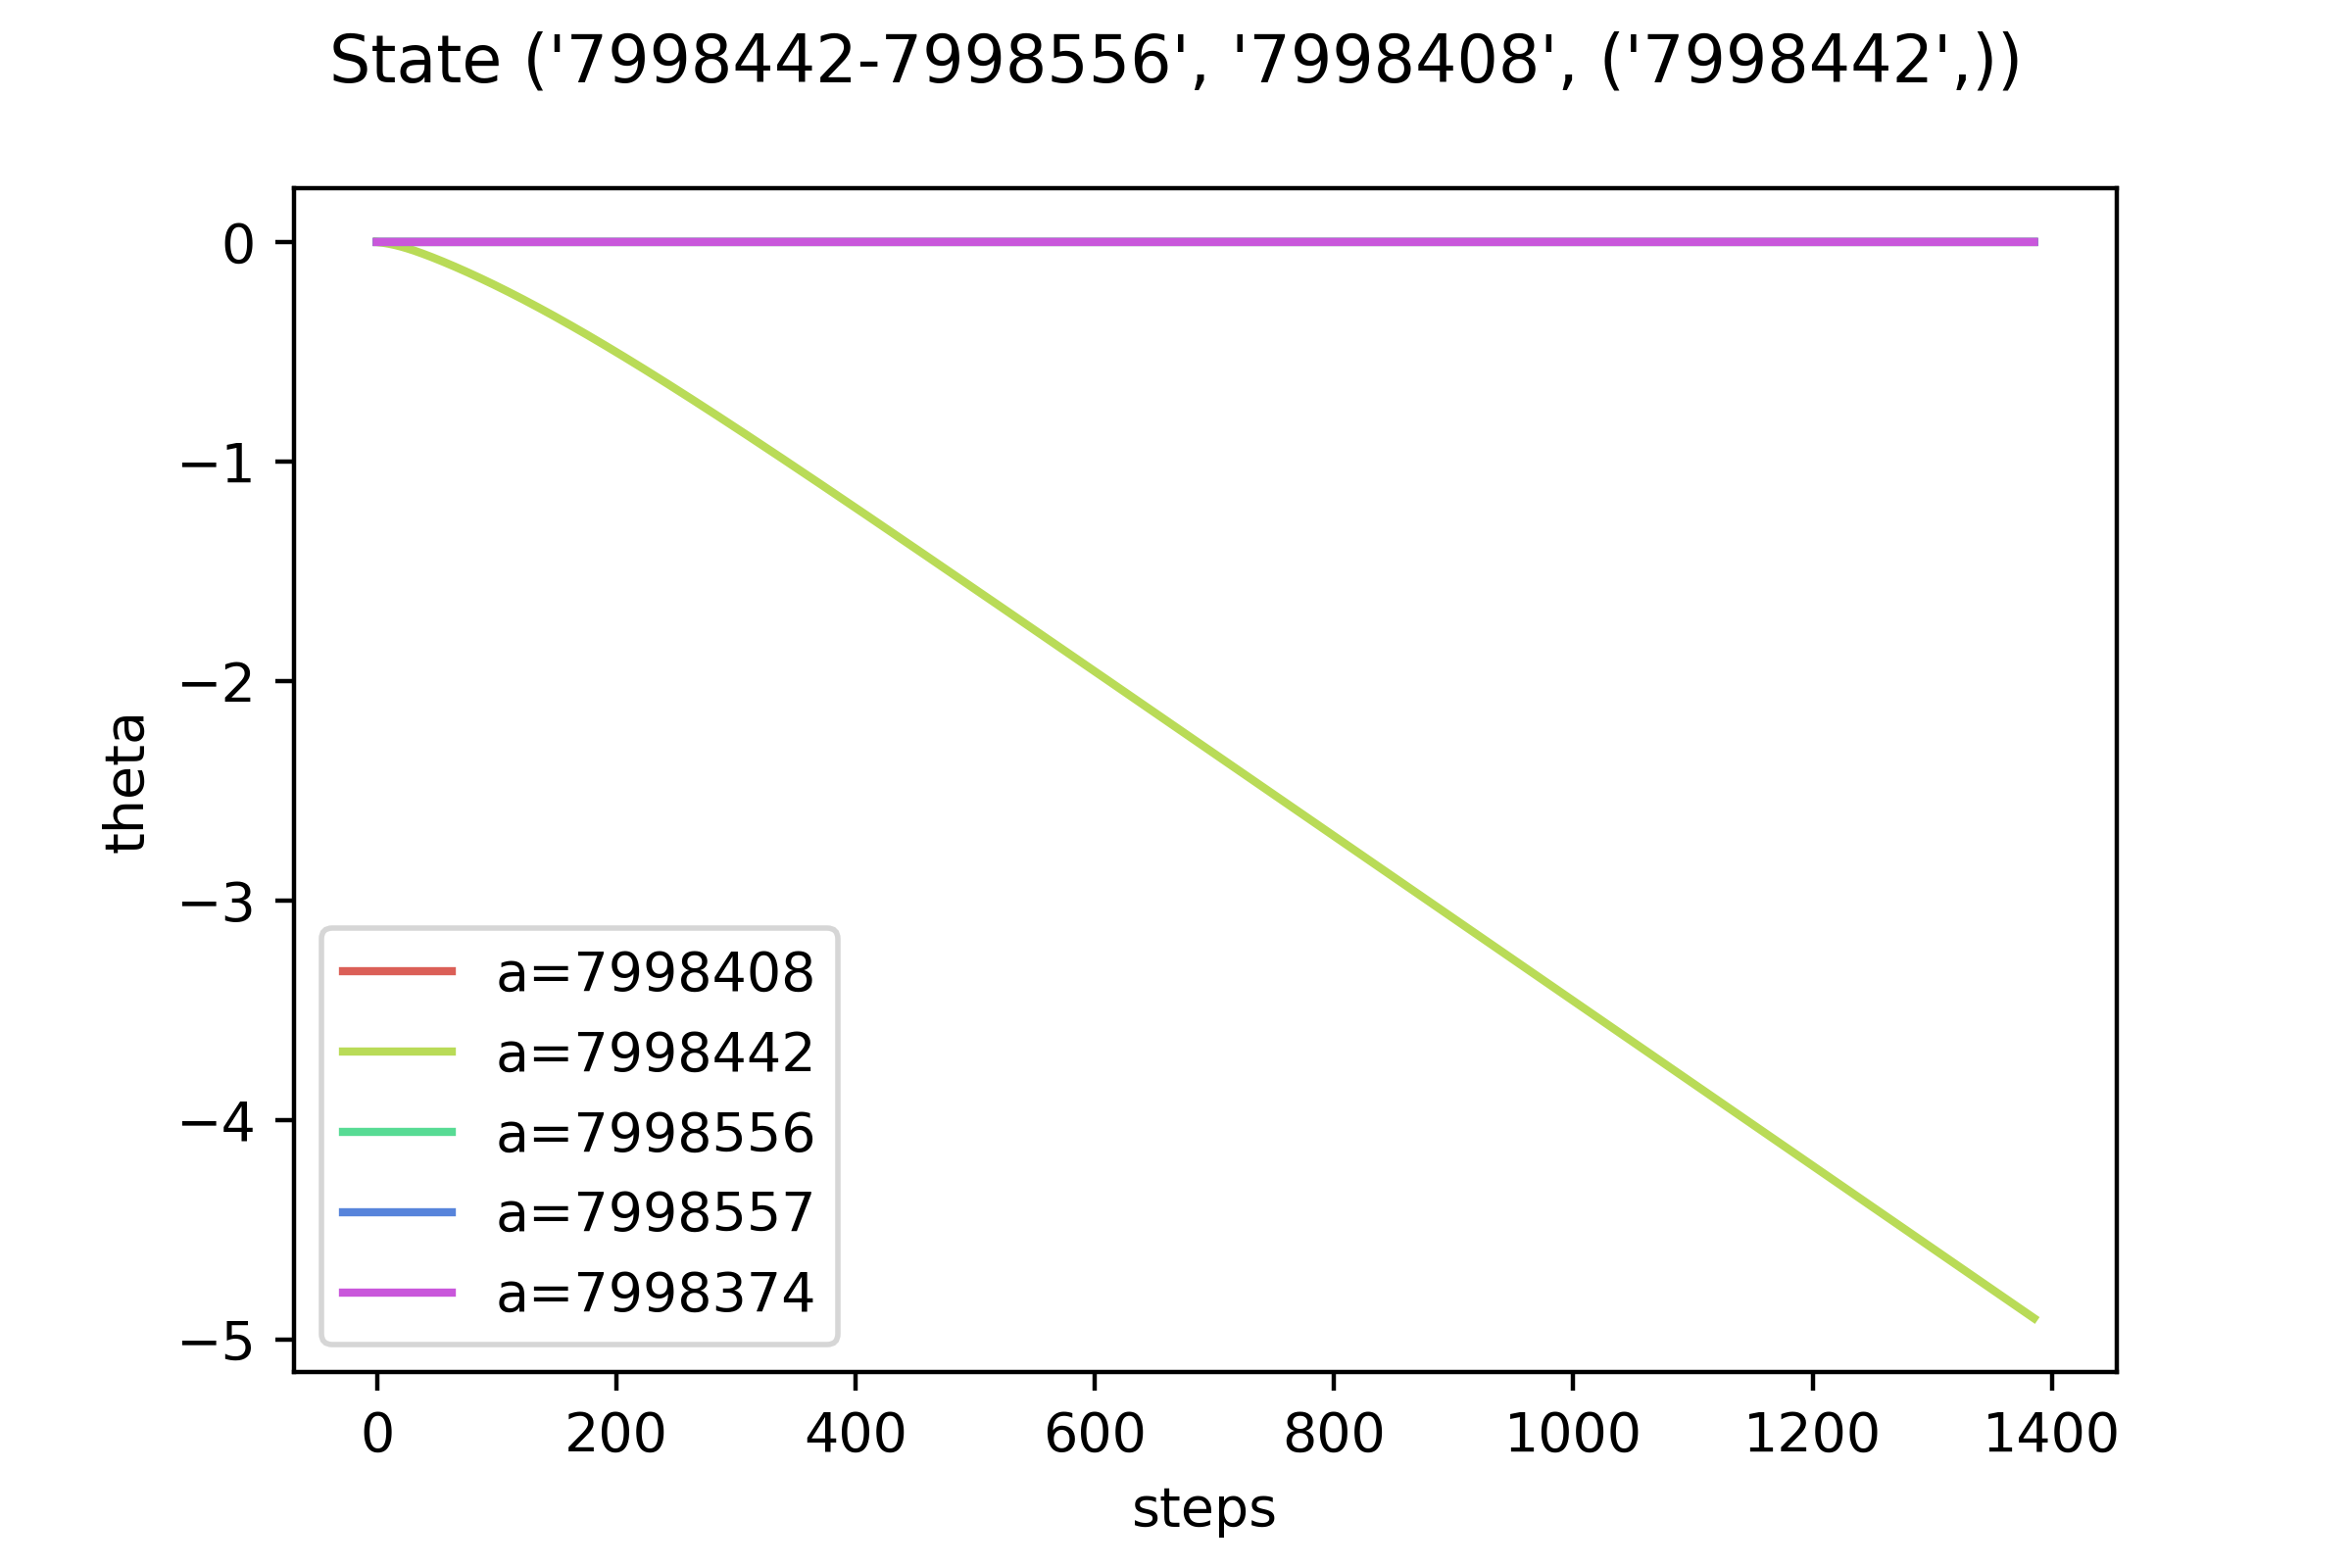
\includegraphics[height=0.27\textwidth,valign=b]{chapters/figures/theta_NPG_state_2.png} &
        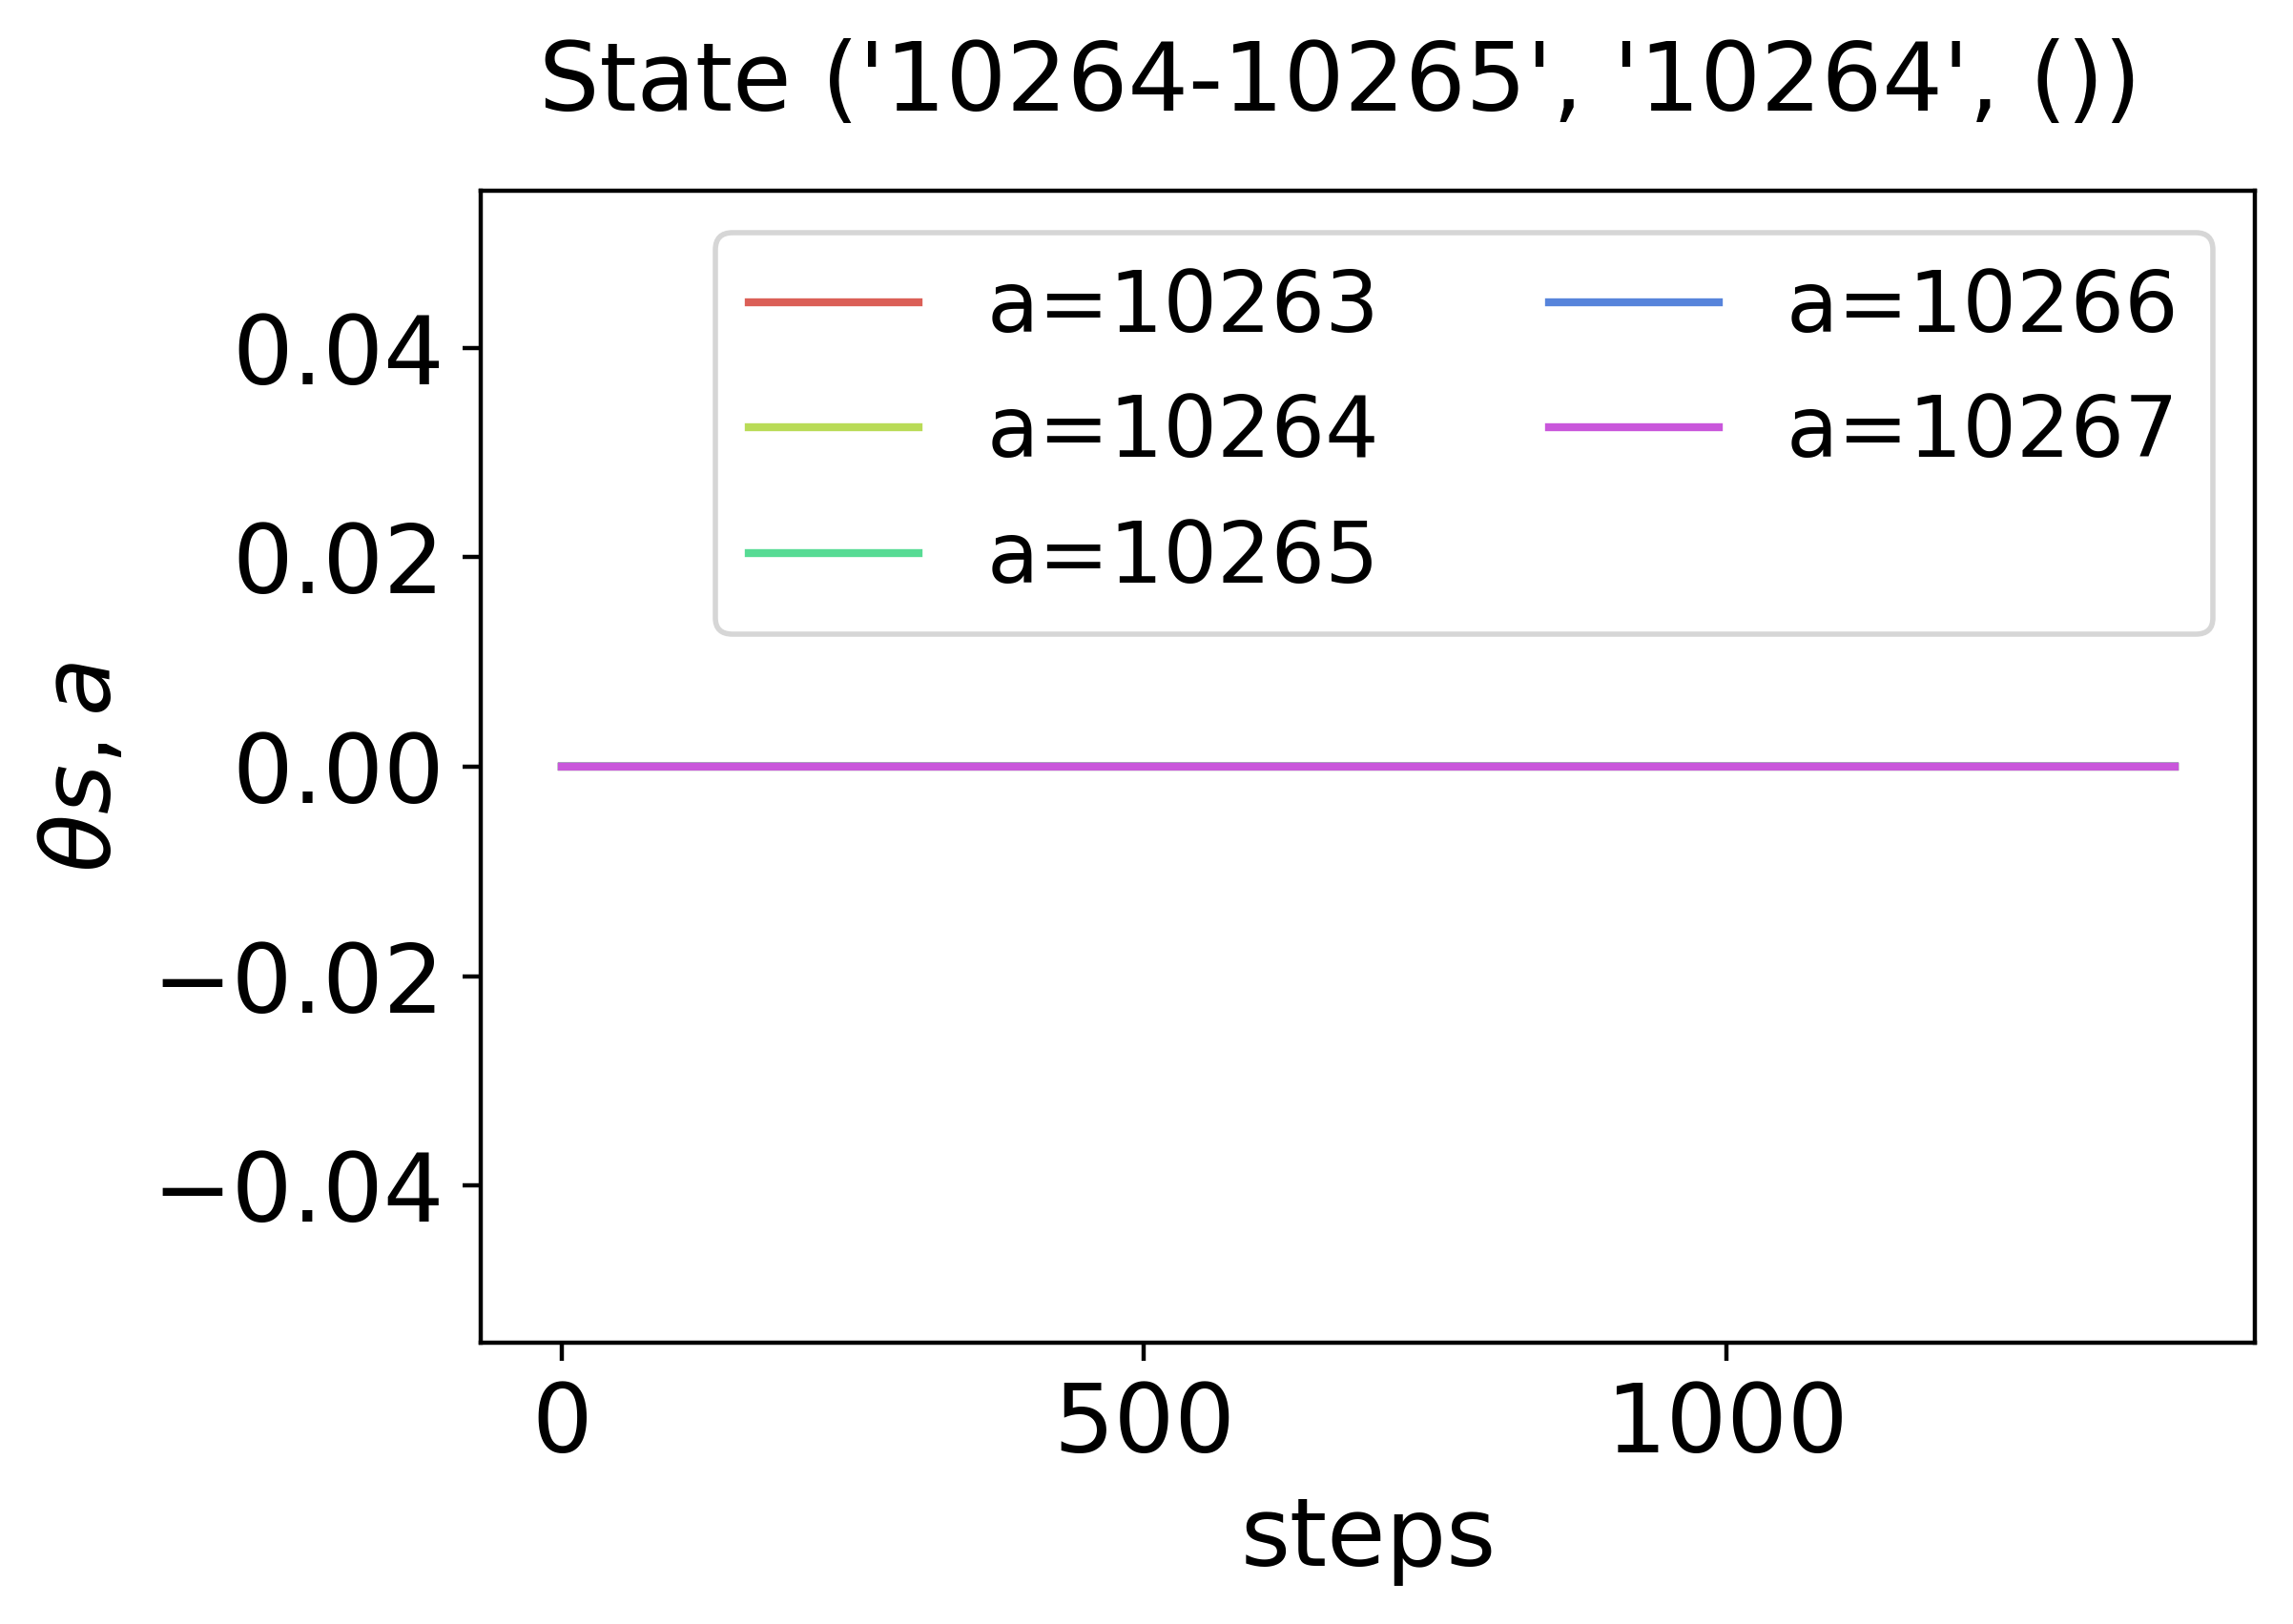
\includegraphics[height=0.27\textwidth,valign=b]{chapters/figures/theta_NPG_state_3.png}
    \end{tabular}
    \caption{Trajectories of the parameters $\boldsymbol \theta$ in the parameters space for \acrshort{npg}, for a specific episode with $5$ initially disconnected substation.}
    \label{fig:sequence-theta-npg}
\end{figure}

\begin{figure}[!htp]
    \centering
    \begin{tabular}{cc}
        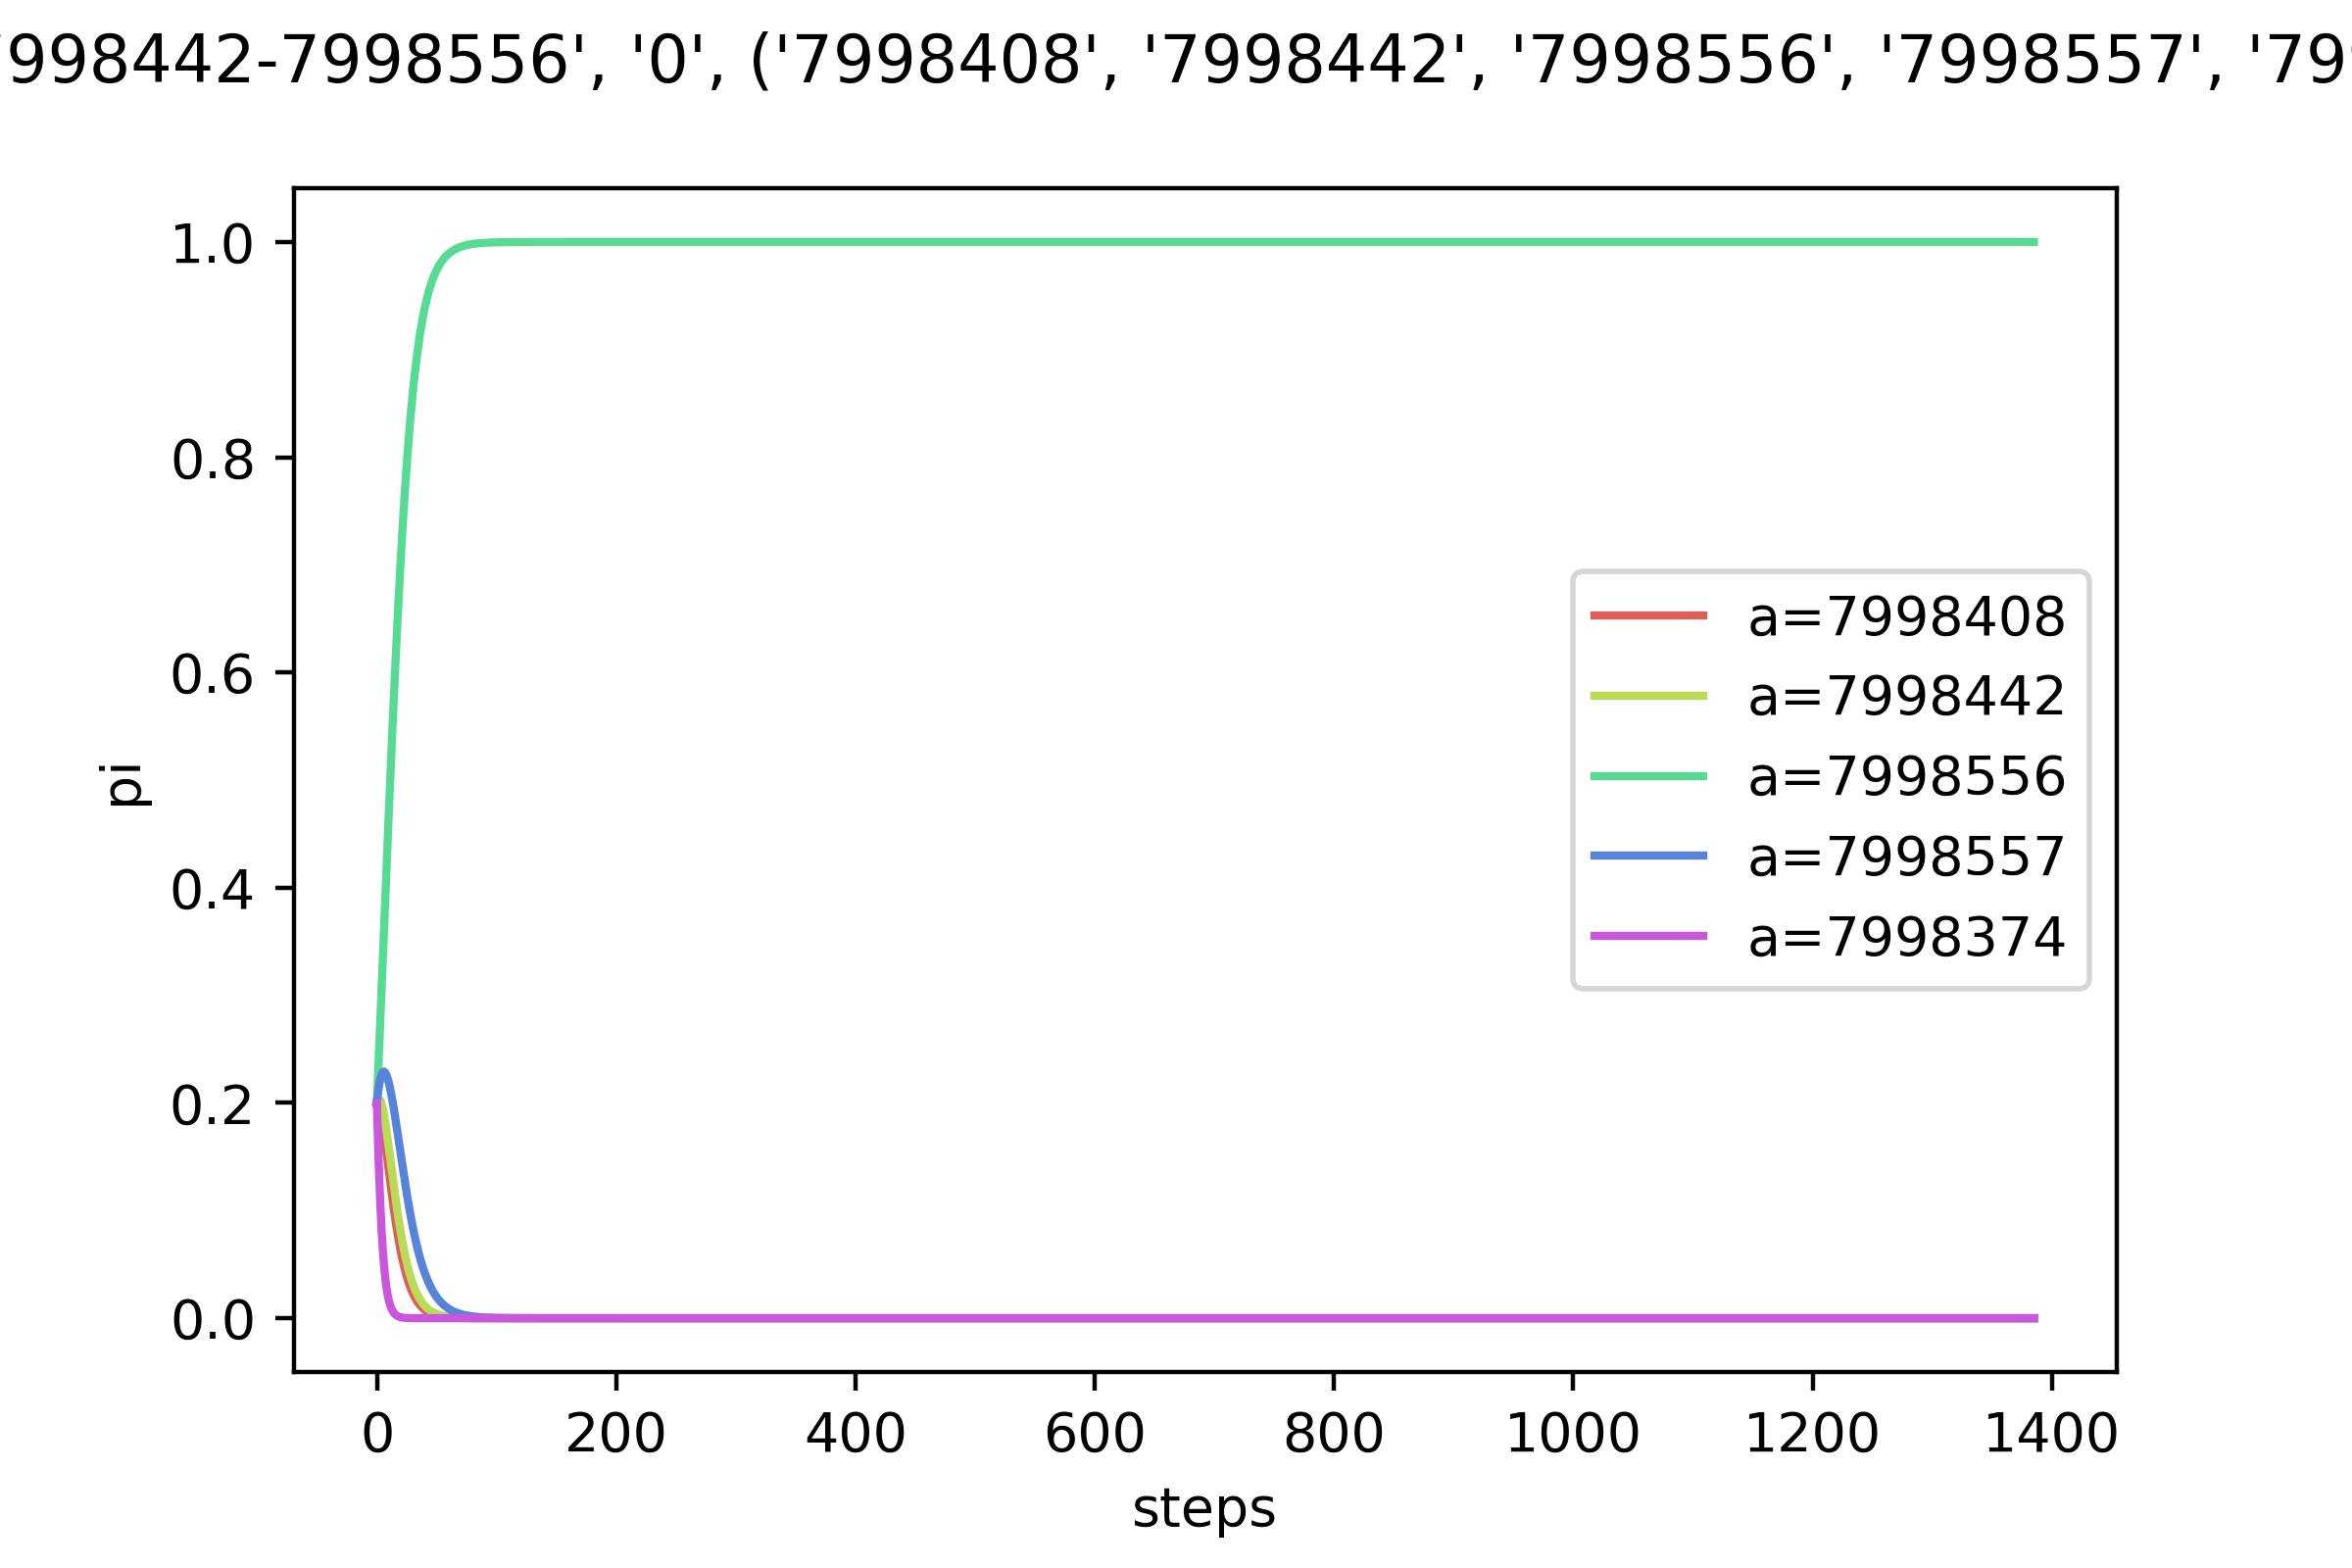
\includegraphics[height=0.27\textwidth,valign=b]{chapters/figures/policy_NPG_state_0.png} &
        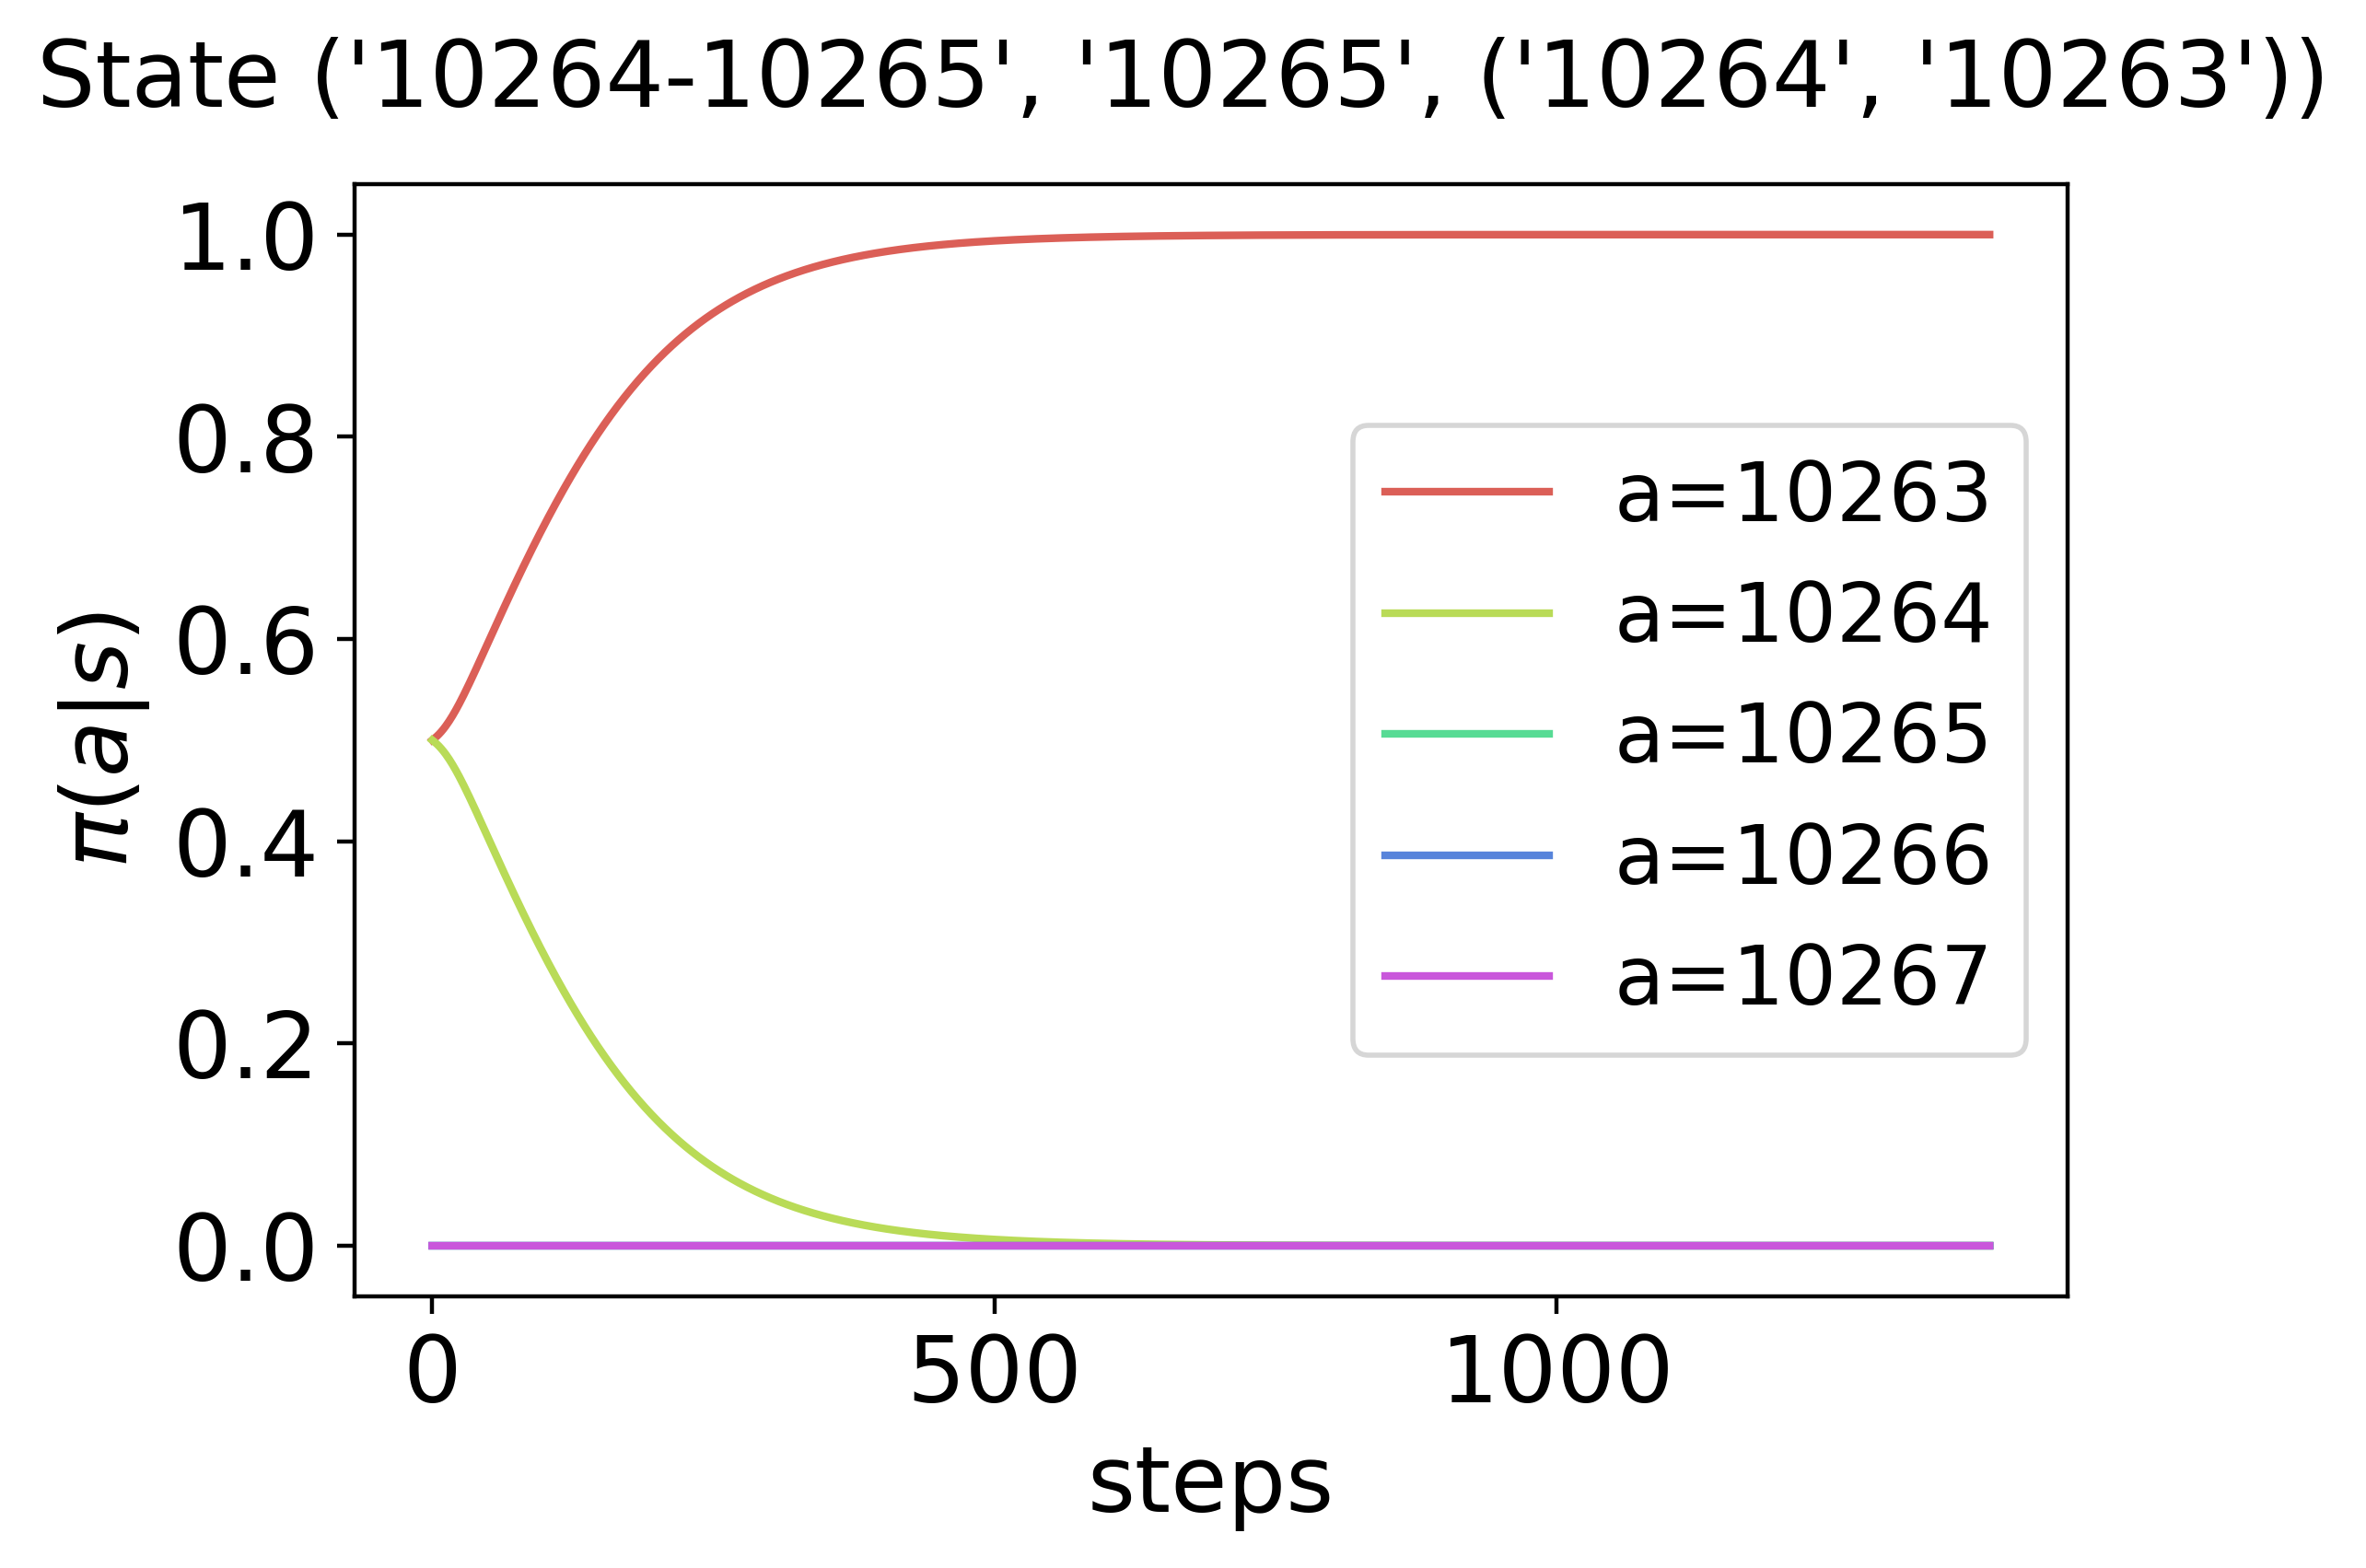
\includegraphics[height=0.27\textwidth,valign=b]{chapters/figures/policy_NPG_state_1.png} \\
        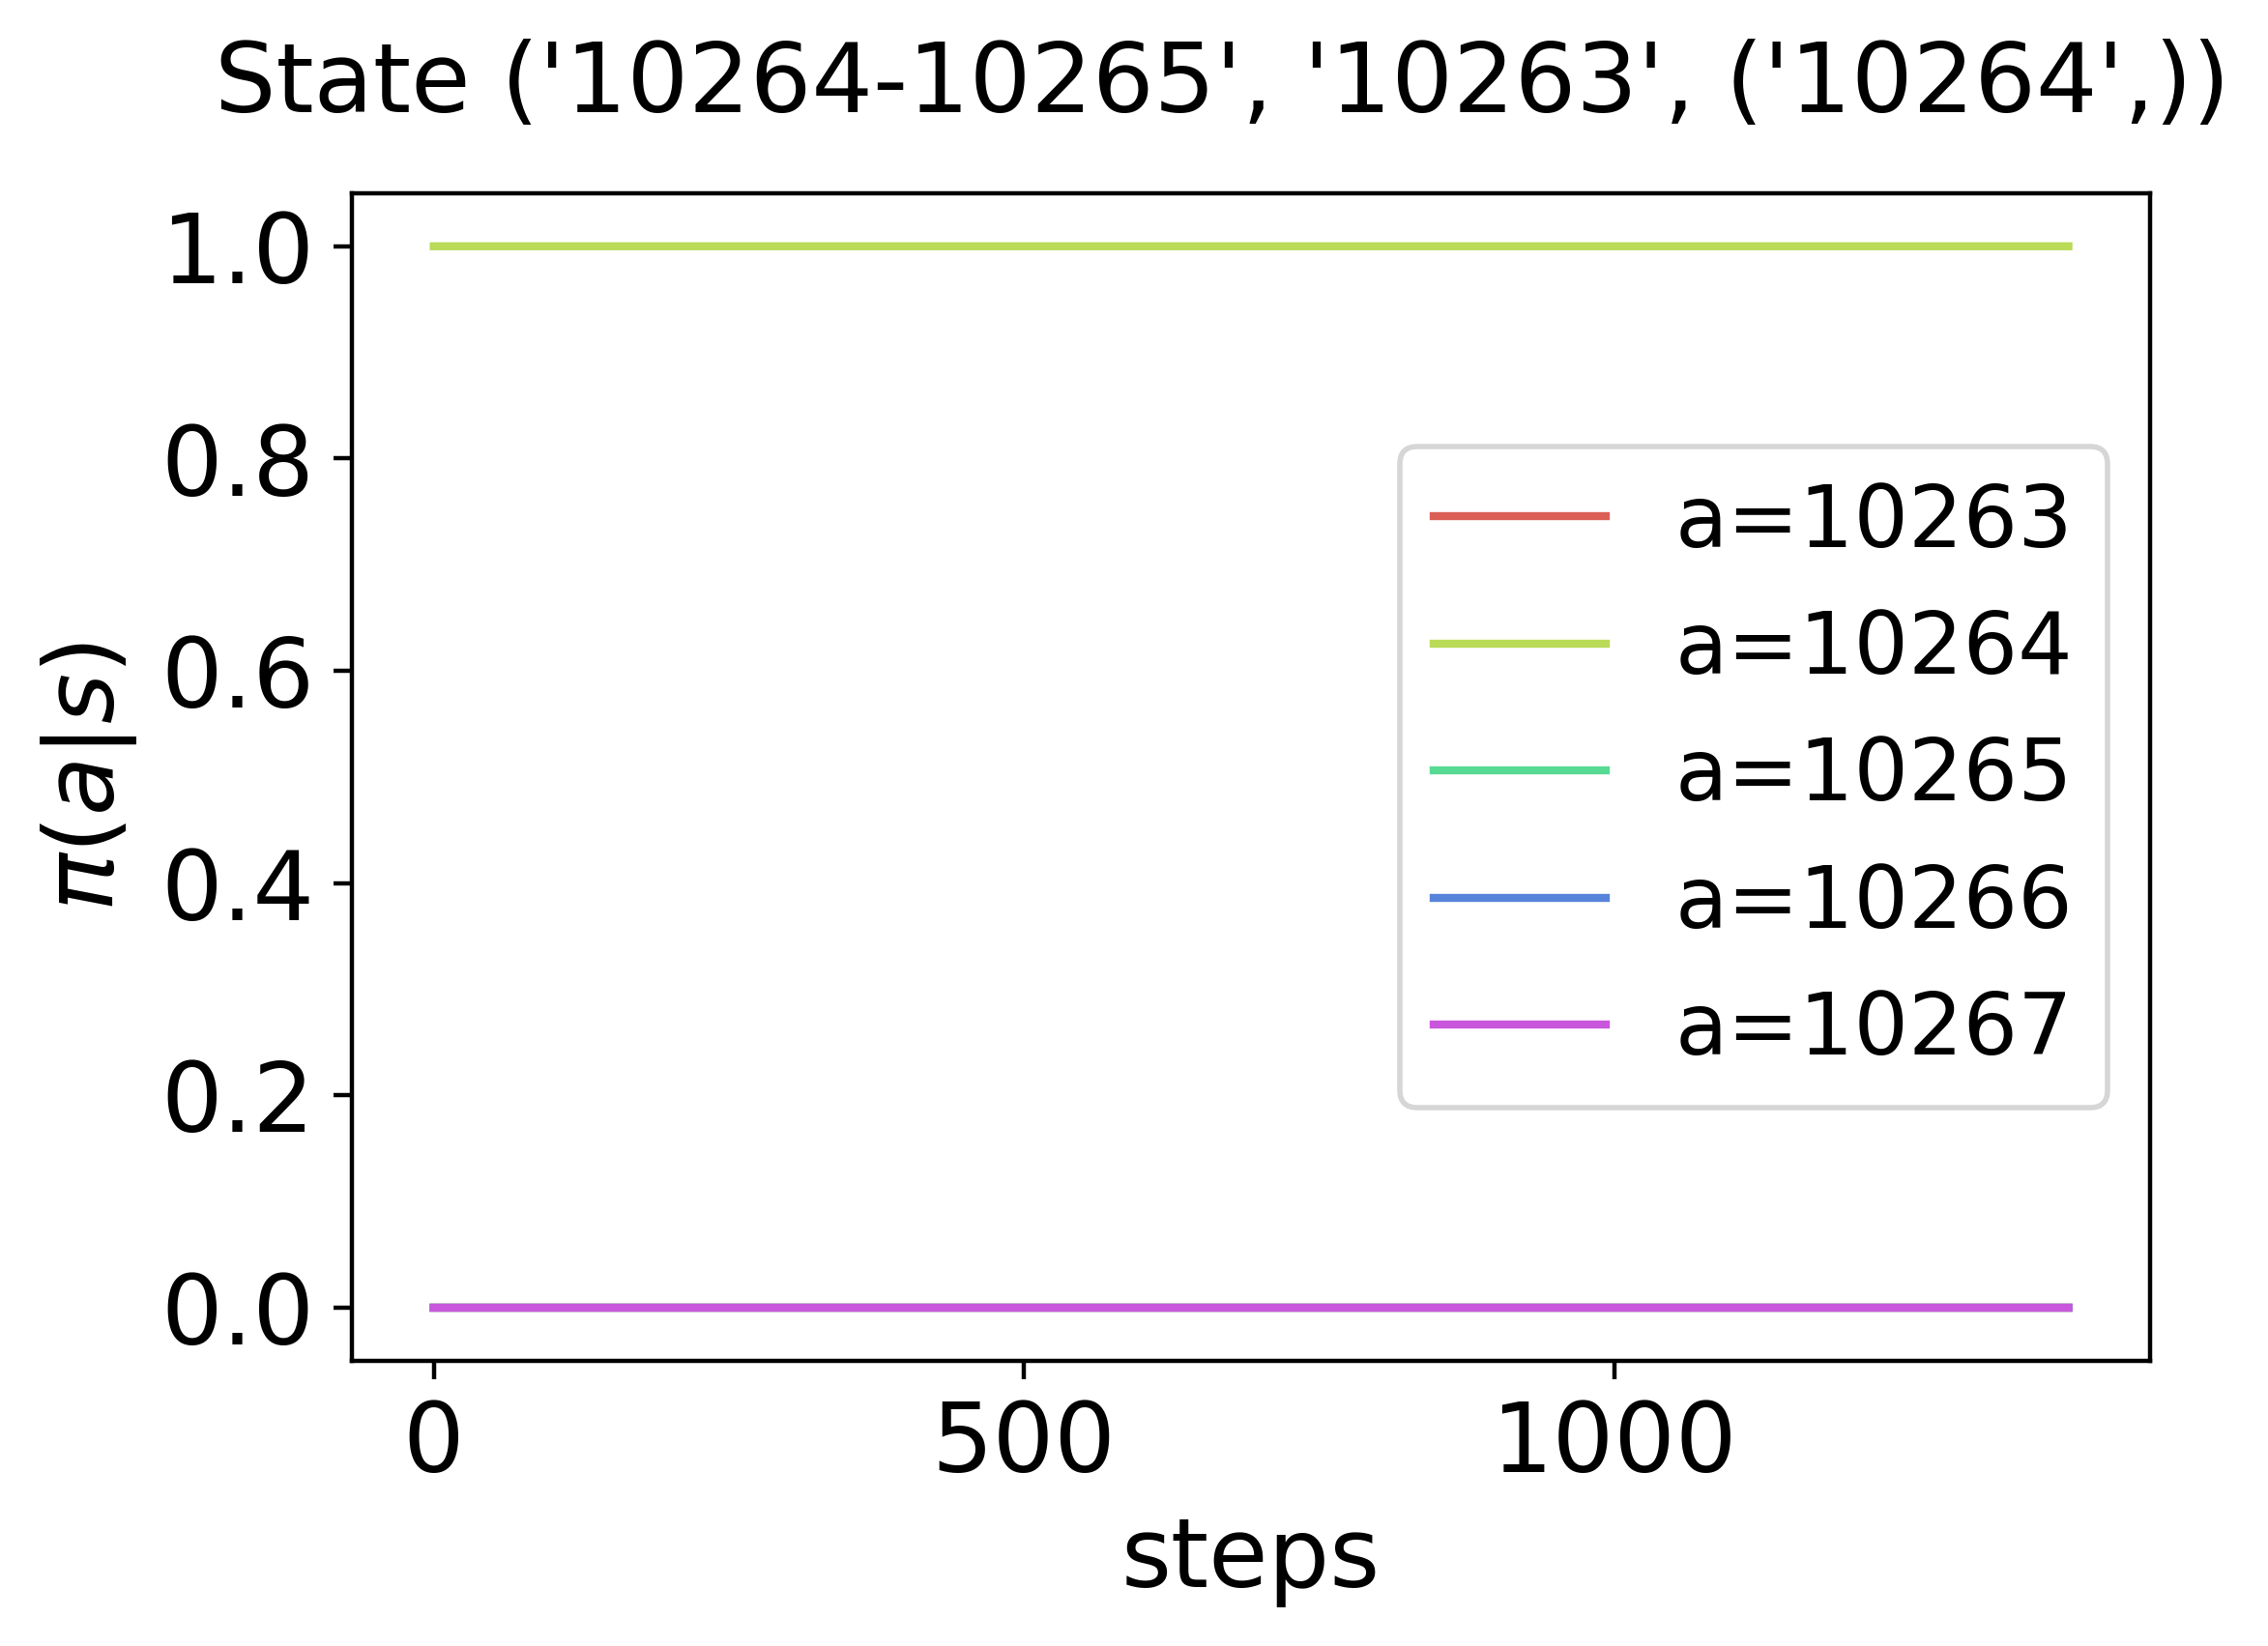
\includegraphics[height=0.27\textwidth,valign=b]{chapters/figures/policy_NPG_state_2.png} &
        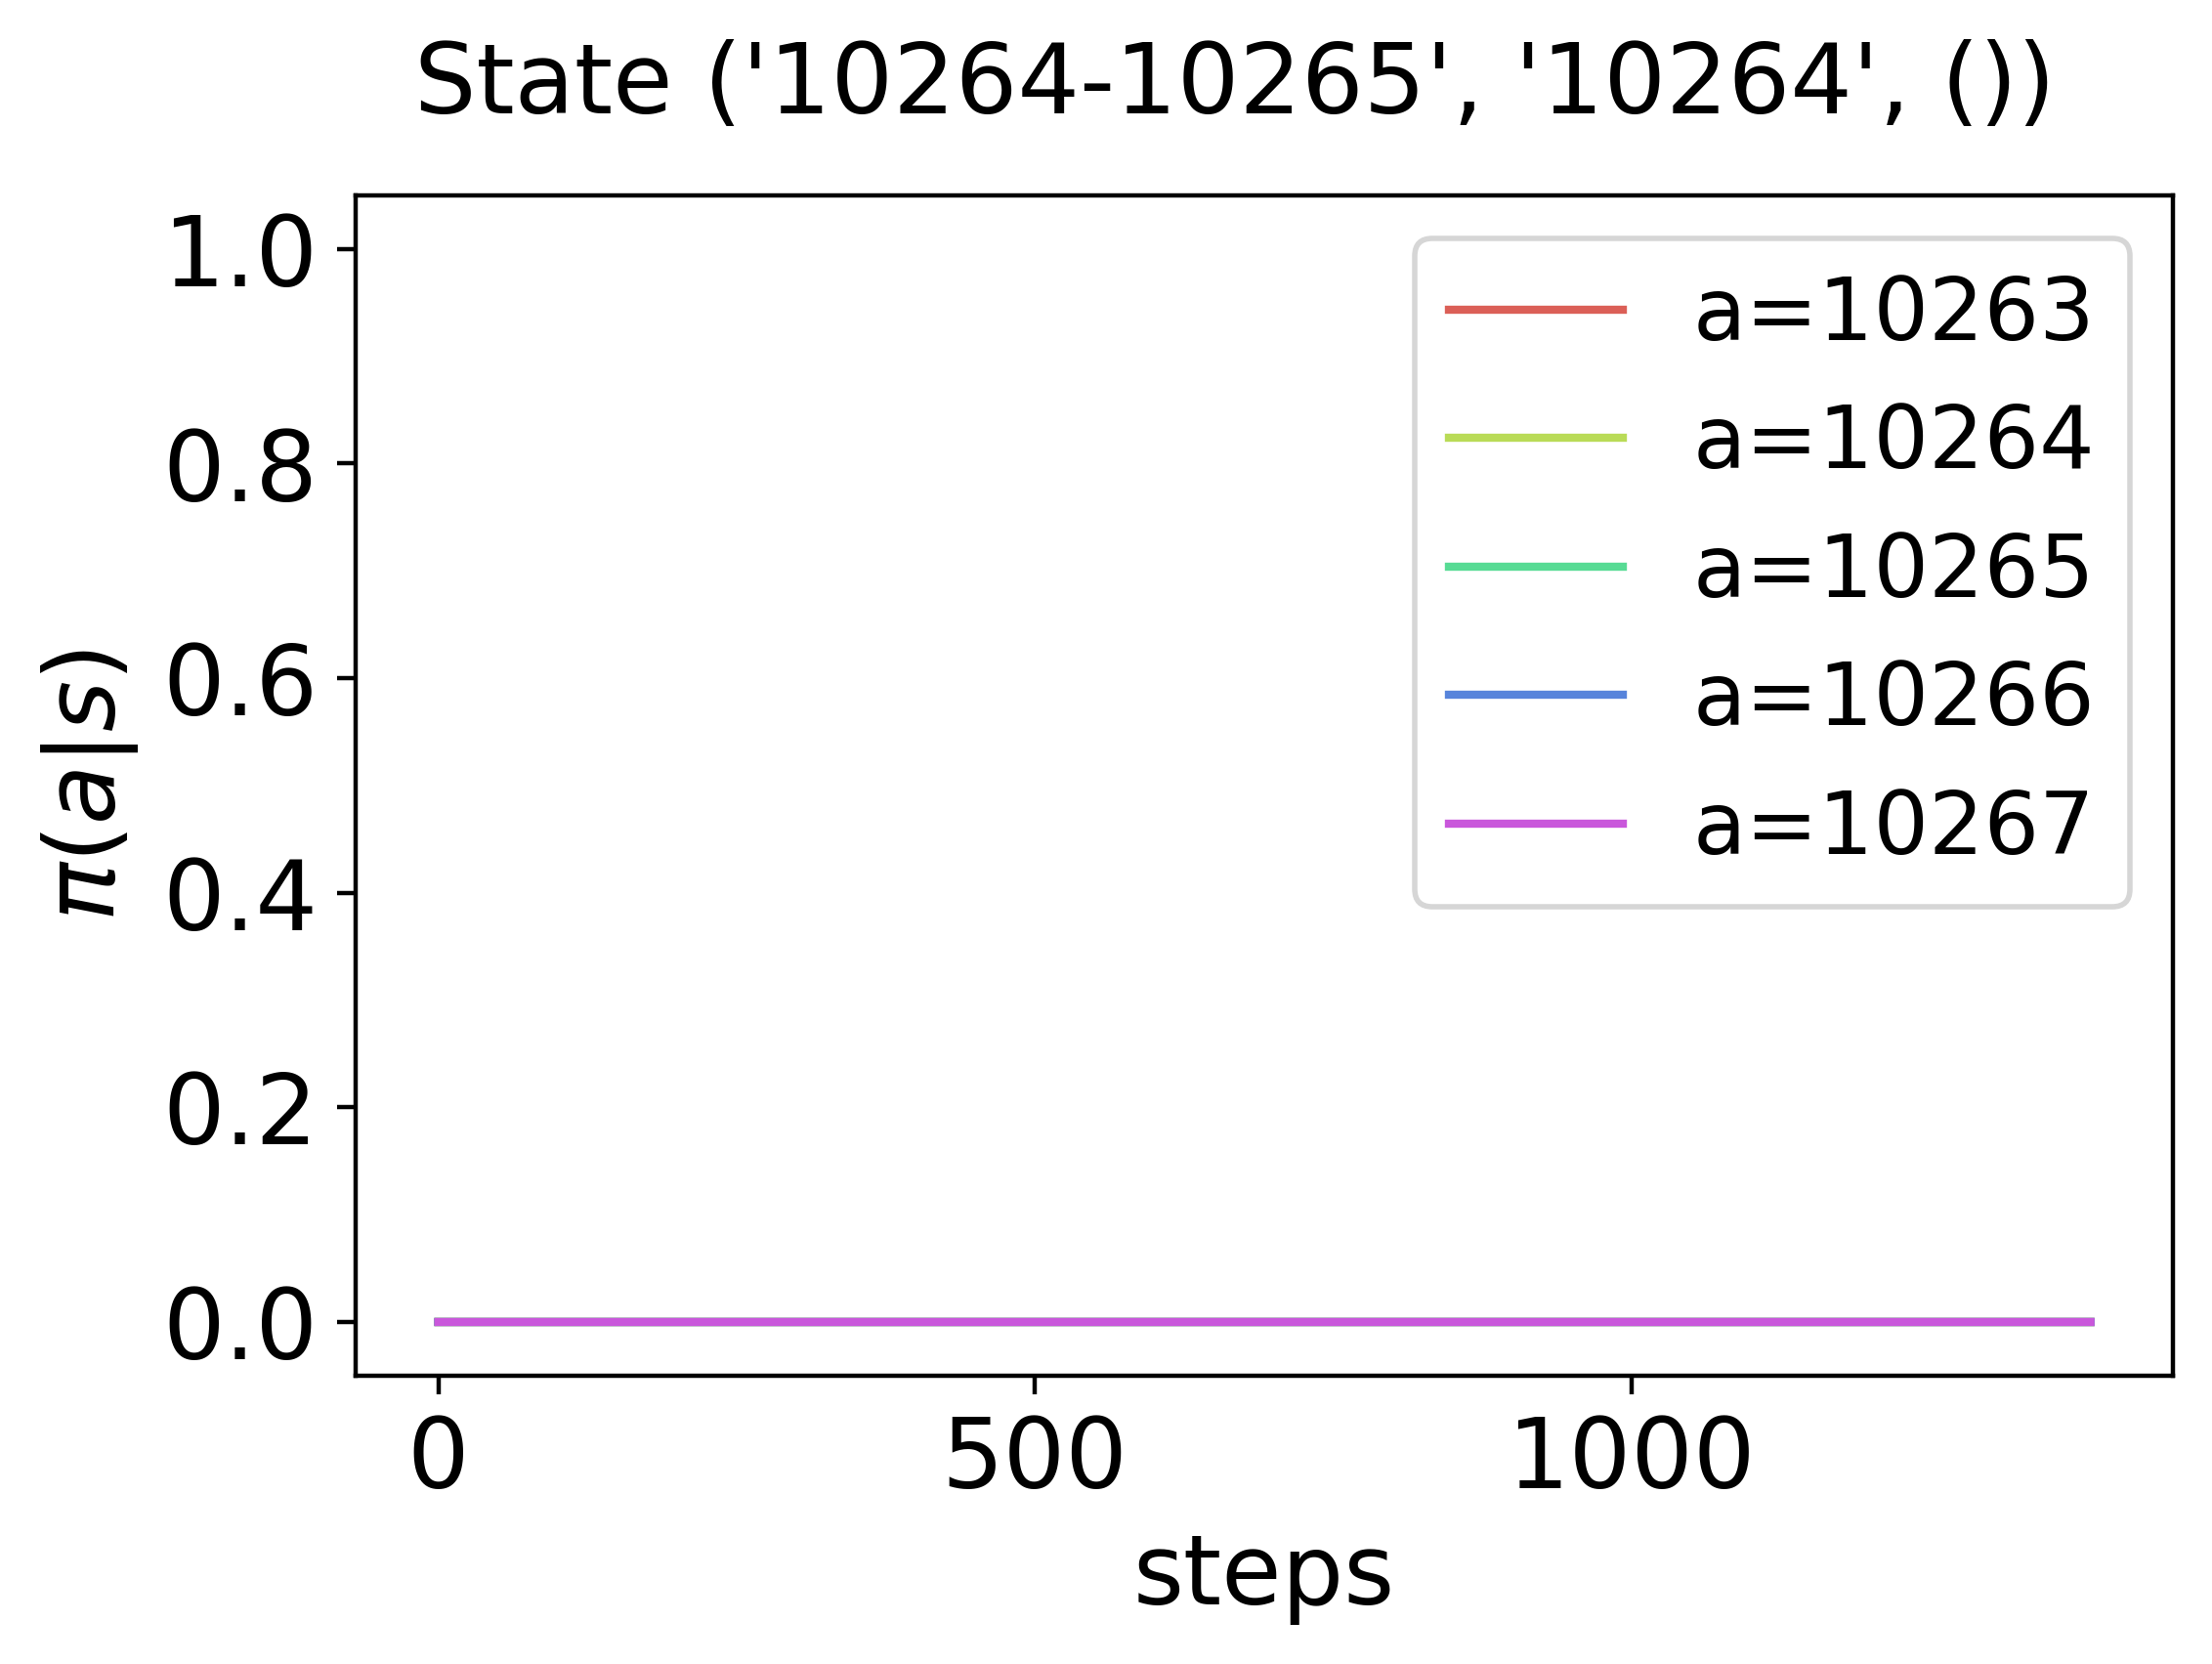
\includegraphics[height=0.27\textwidth,valign=b]{chapters/figures/policy_NPG_state_3.png}
    \end{tabular}
    \caption{Trajectories of the policies $\pi_{\boldsymbol \theta}$ in the policy space for \acrshort{npg}, for a specific episode with $5$ initially disconnected substation.}
    \label{fig:sequence-policies-npg}
\end{figure}

The most important thing to notice in these figures is that all the trajectories are continuous, without sudden turns backward. Going into more detail, in the \acrshort{pg} trajectories of $\boldsymbol \theta$ we can see that one of the parameters grows to infinity, while the others either decrease to infinity or are zero (the latter correspond to actions that cannot be taken in that state). In particular, in the last panel all parameters are zero, since in the terminal state we cannot take any action. Moreover, in the second to last panel we have that again all $\theta$s are zero, because we only have one possible action, so the corresponding $\theta$ is zero, in order for the soft-max policy to be equal to $1$, while the others are zero because they correspond to inadmissible actions. Instead, in the \acrshort{npg} we have that all the parameters $\boldsymbol \theta$ decrease, since we are not following the steepest direction in the parameters space, but the steepest direction with respect to the Fisher metric. Even with rather different values of the parameters $\boldsymbol \theta$, the policies are the same (when compared among them, the difference is in the order of $10^{-2}$), and from the figures we can see that they reached convergence.

Instead, the classic check of seeing if the gradient reached a zero is not applicable in this case: in fact, since we find a stochastic policy, we are not in a corner of the space, in which the gradient is exactly zero, but we are on a side, so it can have values different from zero. Indeed, this is what happens if we look at the gradient matrix: for some states it is not equal to zero, even significantly.

Another check we performed to assess the convergence is to initialize the \acrshort{npg} algorithm with the parameters $\boldsymbol \theta$ found by the \acrshort{pg} algorithm, and vice versa. What we got is that the \acrshort{npg} continues the gradient descent for about another $600$ step, reducing a bit the value of $J_\pi(\boldsymbol \theta)$. Actually, the difference is in the order of $10^{-4}$, which is around the $0.001\%$, so it is negligible. Instead, the \acrshort{pg} algorithm exits immediately the gradient descent loop, as soon as the check on the error is performed, and the values of $J_\pi(\boldsymbol \theta)$ are identical (with a difference of $10^{-10}$), as well as the policy (with a difference of $10^{-15}$).

To check if we reached a global minimum or a local one, since we face a non-convex problem, we also performed some random restarts, with the parameters $\boldsymbol \theta$ initialized from a standard normal distribution $\mathcal N(0,1)$. What happens is that each time the algorithm converges to the exact same policy, so we are quite confident that we reached a global minimum. The references \cite{Bhandari2019, bhandari2020note} show that, under some specific conditions, the policy gradient performance measure $J_\pi(\boldsymbol \theta)$ has a unique global minimum, even if it is non-convex. Indeed, it excludes that the performance measure can have another minimum that can be reached from a different initial condition. Given our results, our model could be in this class of problems, but we have not verified, as that was not our purpose.

% Fai i grafi con gli stati con i path di bisezione e di policy gradient (intensità colore in base alla probabilità): così si può vedere che sono diversi.

Since we computed the policy matrix for all the various bisection algorithms, we were able to compute the exact value of $J_\pi (\boldsymbol \theta)$ for all of them, and we were able to make an effective comparison among all the algorithms. In \autoref{fig:comparison-graph}, we can see the values of $J_\pi(\boldsymbol \theta)$ computed by the various algorithms for different numbers of initially disconnected substations. We selected an electrical line of Trieste's power grid, and keeping fixed the initial position of the technician and the last remotely controlled substation, we moved the first remotely controlled substation of one substation each time, in order to incrementally increase by one the number of initially disconnected substations.
% Anche nel comparison graph bisognerebbe dire che J è calcolato solo per i guasti sui cavi
We can clearly see that the policy gradient algorithms are the better ones, with the \acrshort{npg} a little better with higher numbers of disconnected substations. Instead, the different bisection algorithms perform almost the same.

\begin{figure}[htb]
    \centering
    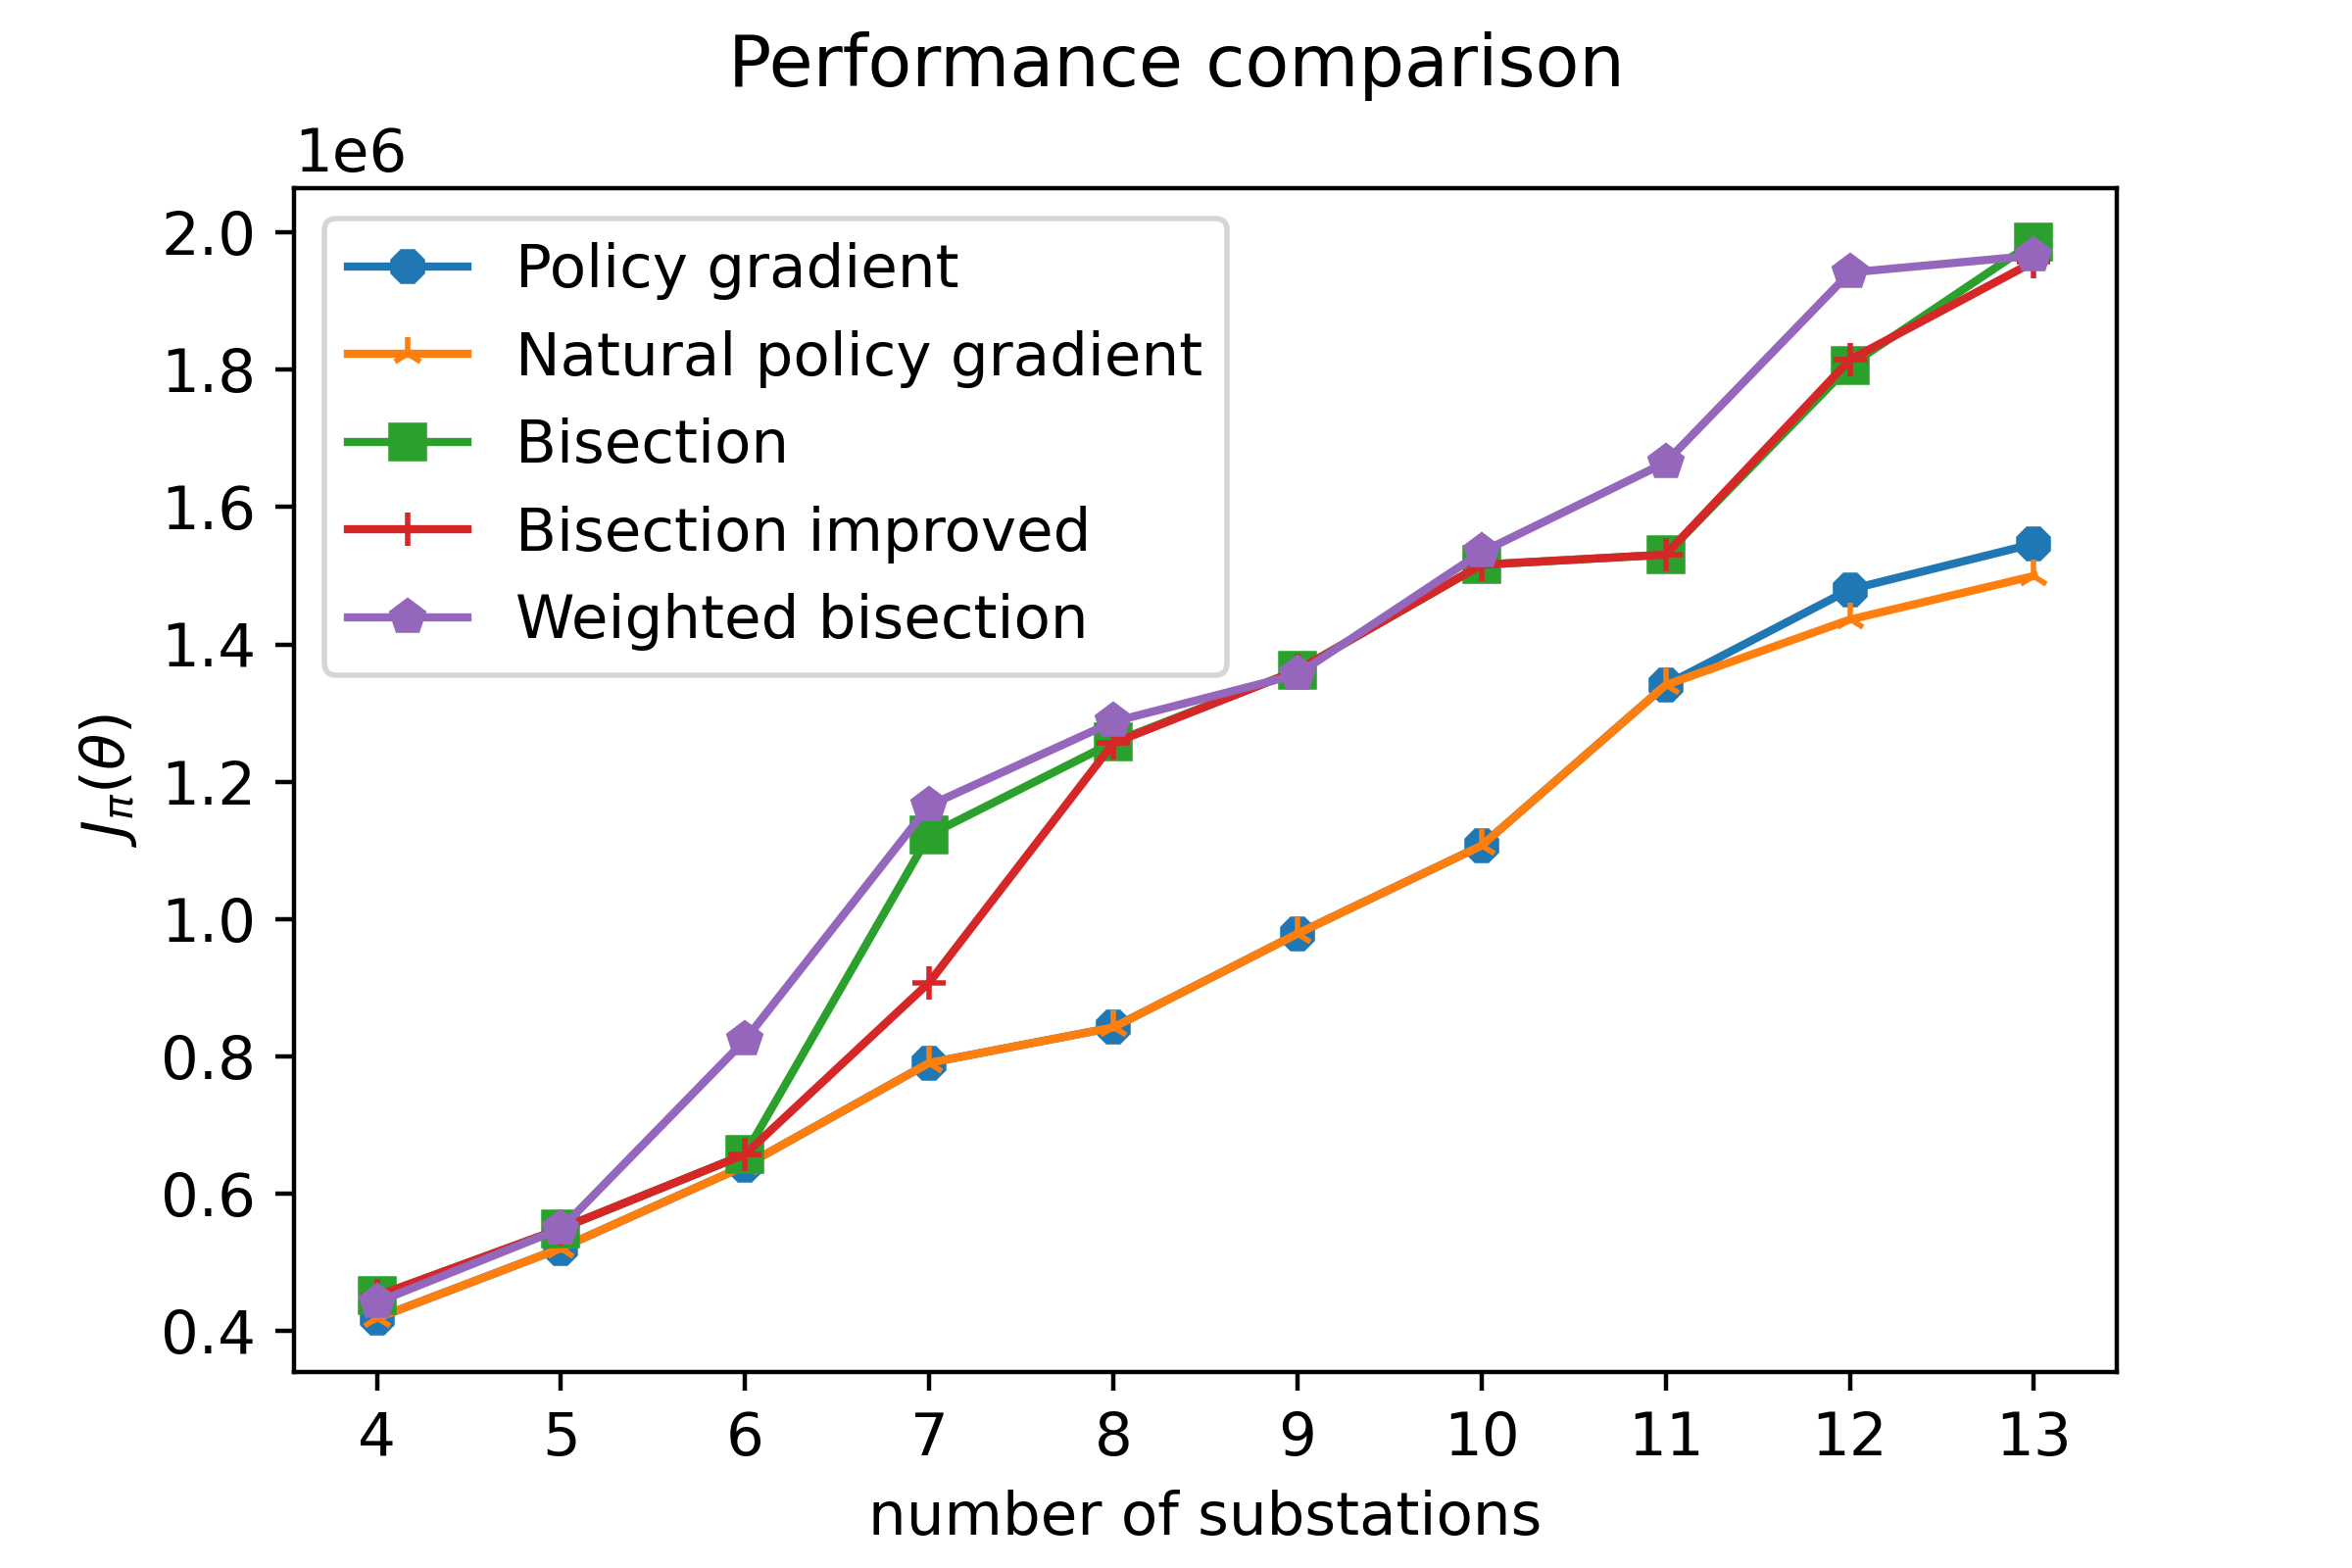
\includegraphics[width=0.8\textwidth]{chapters/figures/comparison_graph.png}
    \caption{Comparison among the various algorithm.}
    \label{fig:comparison-graph}
\end{figure}

In \autoref{fig:scatterplot} we can see a plot of the costs for different positions of the fault of the \acrshort{pg} and the bisection algorithms. We considered only the faults on the electrical cables, otherwise there would have been too many points, and since according to the data collected by the technicians they are the most frequent ones, thus they are the most representative. We have indicated with \texttt{f1} the fault between the first remotely controlled substation and the first disconnected substation, with \texttt{f2} the fault between the first and the second disconnected substations, with \texttt{f3} the fault between the second and the third disconnected substations, and so on so forth.

\begin{figure}[htb]
    \centering
    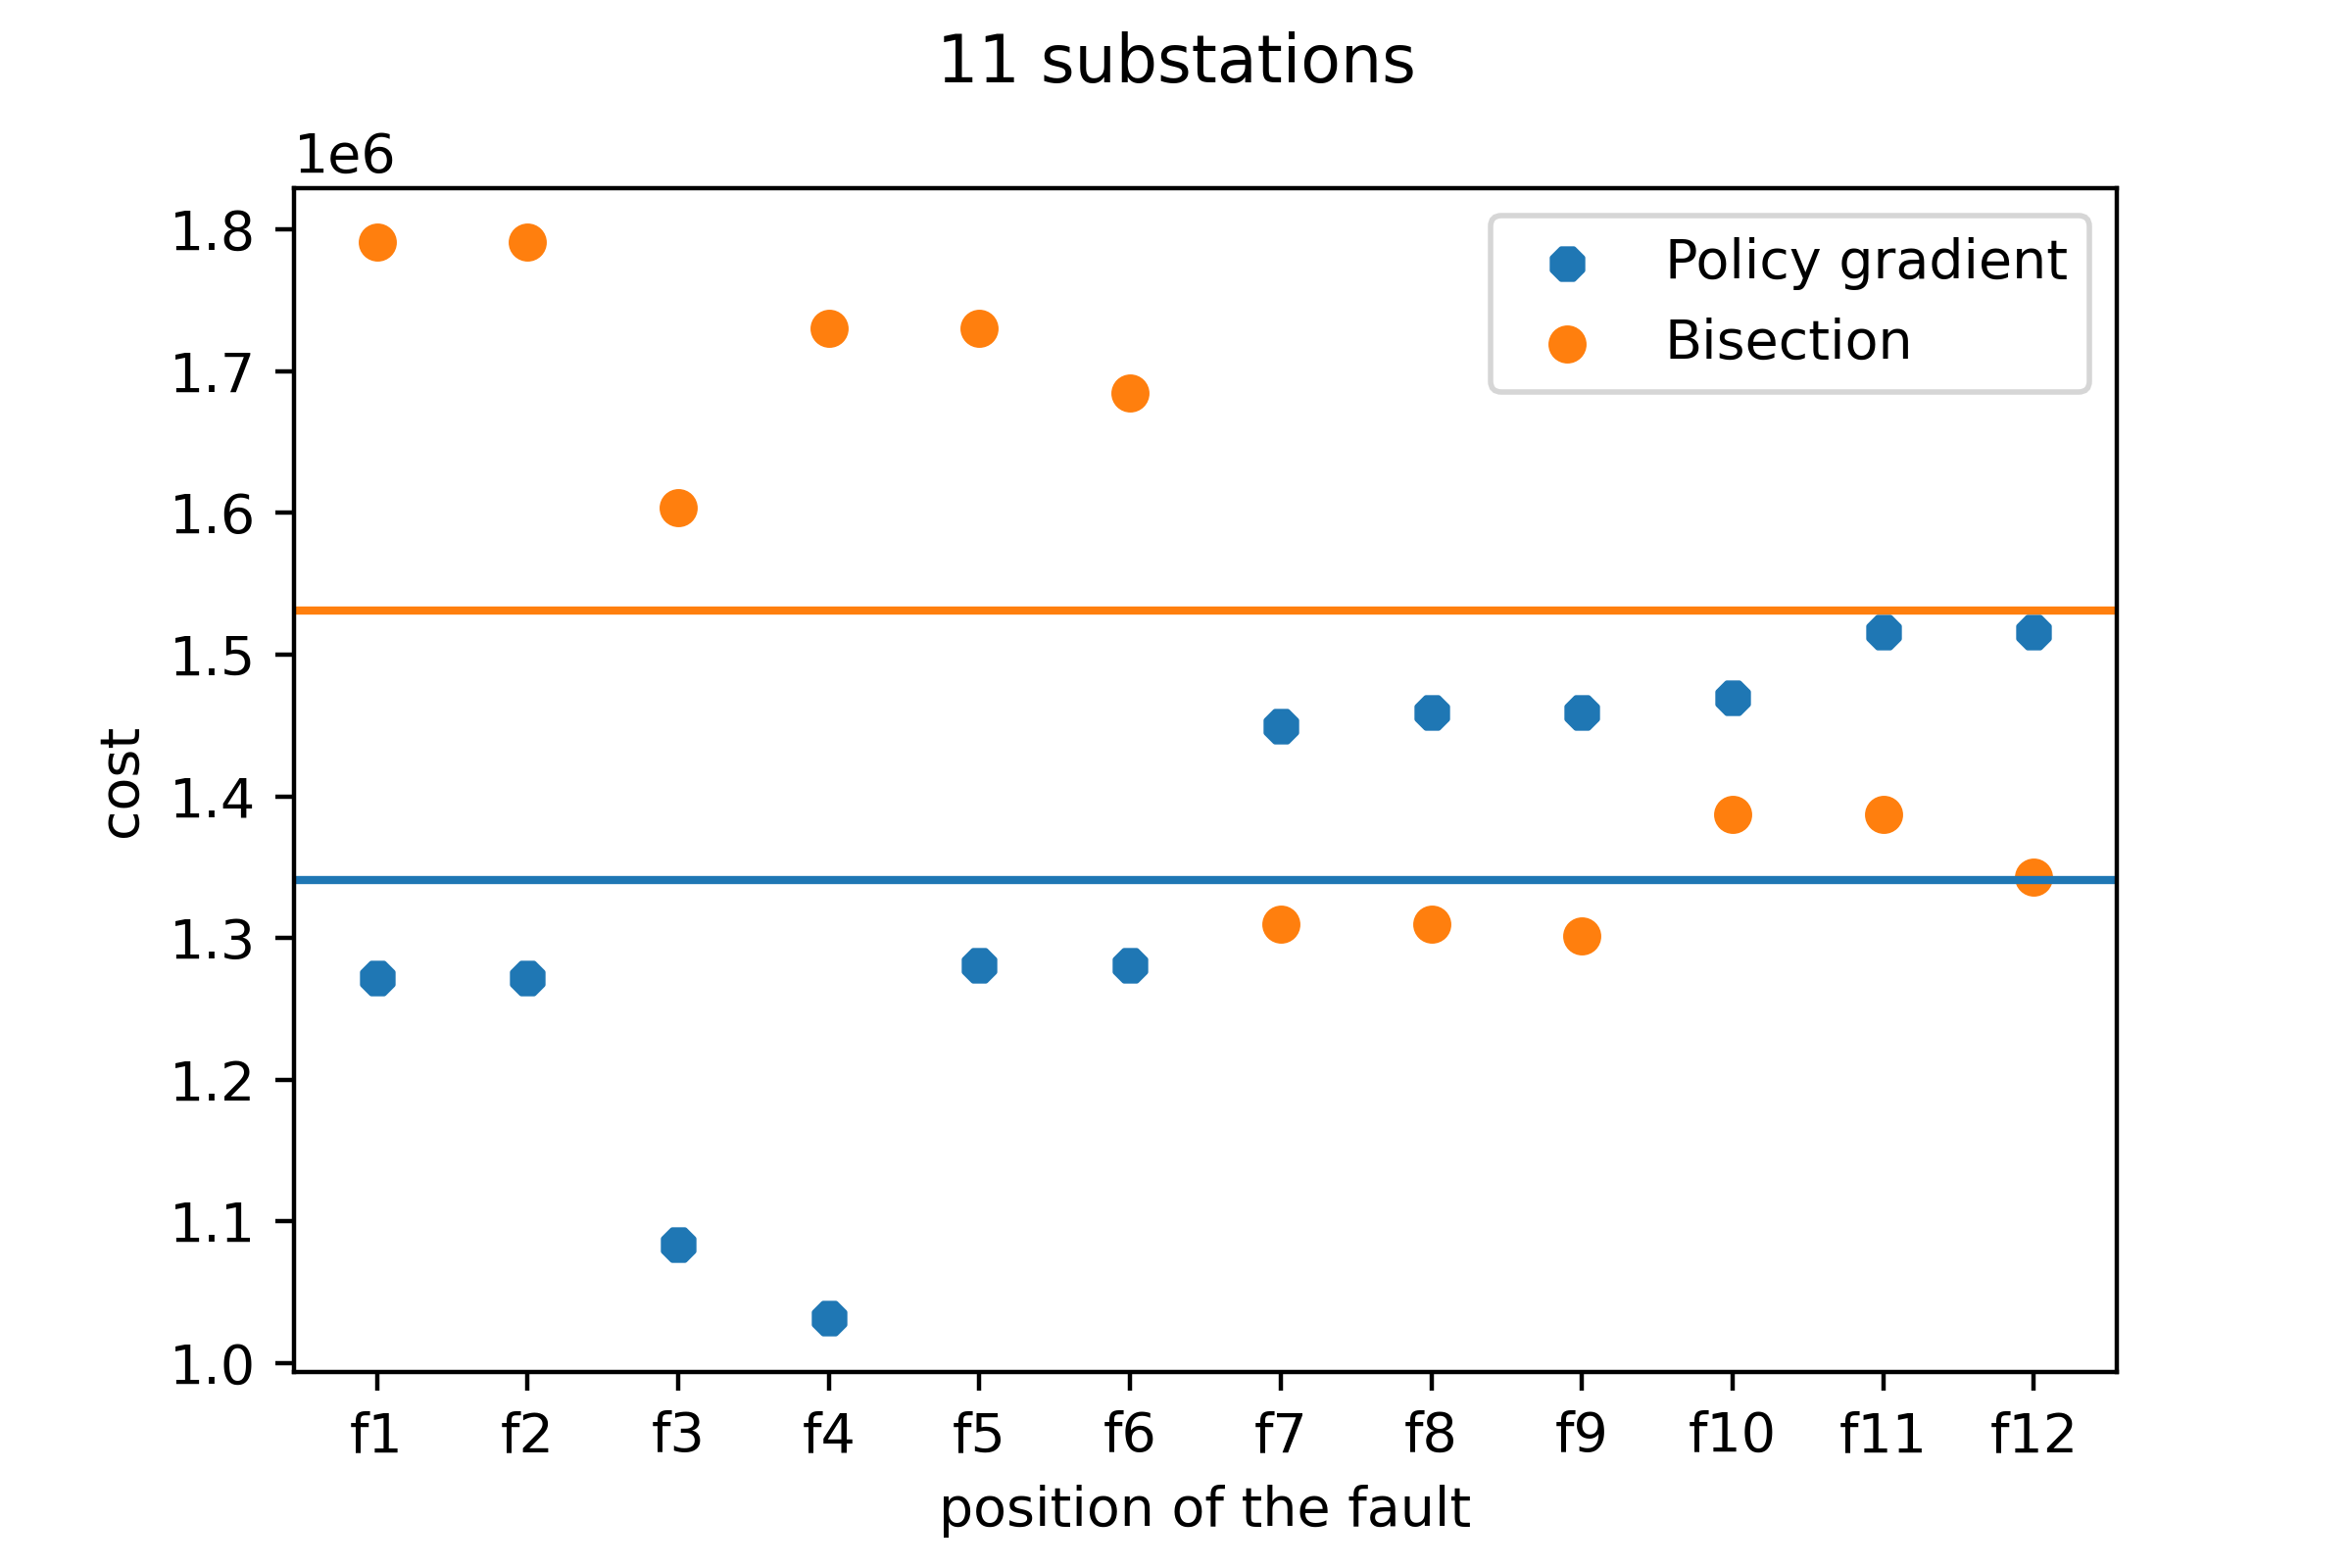
\includegraphics[width=0.8\textwidth]{chapters/figures/scatterplot.png}
    \caption{Costs for different positions of the fault.}
    \label{fig:scatterplot}
\end{figure}

\section{Conclusion}

We have succeeded in developing a method that reaches, on average, a better solution than the current one used by the technicians. But it is possible that, using a different cost structure, these results do not remain the same. The performances of the heuristic technique and the policy gradient algorithm may increase or decrease if we change the definition of the cost. However, it is remarkable that even in this case our algorithm would continue to be applicable and scalable. In fact, besides our specific results, what is important is to have developed a method that can find systematically an optimal policy in the model-based context, in which we know the consequences of our actions.

Another possible approach would be to use a model of \emph{mixed integer (linear) programming}, where only some unknown variables are required to be integers, while the others are continuous. In this case, it is possible to cerchiamo di minimizzare il caso peggiore \colorbox{yellow}{!!!!}

In real life, though, the costs are not quite like we modeled them, they are much more random, since they depend on many factors: whether it is day or night, whether the instrumental test is applicable, the weather conditions, and, of course, many other unexpected events can happen. If we are to model more accurately these costs, first of all we would have to collect data on them, using maybe a Telegram bot connected to an \acrshort{aws} server, with which the technicians can interact while solving the fault. Then a whole other class of algorithms would be needed to solve this problem: the \emph{model-free}\index{model-free} ones, specifically designed to handle these uncertainties about the costs. This would be an interesting direction for future works, but we will not cover it in the current one.


% Full bibliography
%\bibliographystyle{plain}
%\bibliography{references}
\printbibliography[heading=bibintoc]%[resetnumbers=true]%[notcategory=publist]


% Index
\printindex

\end{document}